\documentclass[11pt,a4paper]{article}
% Shared preamble for every section of the v3.0 paper. Do not redefine these macros in a section file.
\usepackage[T1]{fontenc}
\usepackage[utf8]{inputenc}
\usepackage{lmodern}
\usepackage[margin=26mm,headheight=14pt]{geometry}
\usepackage{amsmath,amssymb,amsthm,mathtools,bm}
\usepackage{microtype,booktabs,array,enumitem,fancyhdr,xcolor,longtable,graphicx}
\usepackage[hyphens]{url}
\definecolor{inklink}{HTML}{51426B}
\usepackage[colorlinks=true,linkcolor=inklink,citecolor=inklink,urlcolor=inklink,pdfauthor={}]{hyperref}
\numberwithin{equation}{section}
\newtheorem{theorem}{Theorem}[section]
\newtheorem{lemma}[theorem]{Lemma}
\newtheorem{proposition}[theorem]{Proposition}
\newtheorem{corollary}[theorem]{Corollary}
\theoremstyle{remark}\newtheorem{remark}[theorem]{Remark}
\theoremstyle{definition}\newtheorem{definition}[theorem]{Definition}
% --- symbols inherited from v2.0 ---
\newcommand{\R}{\mathbb R}
\newcommand{\avg}[1]{\left\langle #1\right\rangle}
\newcommand{\dd}{\,\mathrm dt}
\newcommand{\cP}{\mathcal P}      % oscillatory parameter domain {k>mu(1+mu)}
\newcommand{\cN}{\mathcal N}      % neutral parameter set
\newcommand{\cS}{\mathcal S}
\DeclareMathOperator{\tr}{tr}
\DeclareMathOperator{\spr}{spr}
\DeclareMathOperator{\diag}{diag}
\DeclareMathOperator{\diver}{div}
\DeclareMathOperator{\inter}{int}
\DeclareMathOperator{\sign}{sign}
% --- new global symbols (v3.0) ---
\newcommand{\cA}{\mathcal A}                 % global attractor = union of log-bounded entire orbits
\newcommand{\Dom}{\mathcal D_{\mu,k}}        % chemical domain {x>0,y>0,p<lambda}
\newcommand{\Dsc}{\mathsf D}                 % projection of the attractor to the (U,p) plane
\newcommand{\Dt}{\mathbb D}                  % derivative along the flow of a function of the state
\newcommand{\kH}{k_{\mathrm H}}              % Hopf value mu(1+mu)
\newcommand{\LamE}{\Lambda_E}                % (y-k)-zeta_E U+eta_E p
\newcommand{\Sg}{\Sigma}                     % star gauge  p^2-U p'
\newcommand{\Xg}{\Xi}                        % convexity gauge  p'^2-p p''
\newcommand{\etaz}{\eta_0}                   % explicit state function with mean mu
\newcommand{\psiU}{\psi}                     % psi(U)=U e^U-e^U+1
\newcommand{\Rem}{\mathcal R}                % R(d)=e^d-1-d
\setlength{\parskip}{3pt}
\setlength{\parindent}{1.2em}
\setlist{nosep,leftmargin=1.7em}

\hypersetup{pdftitle={Convex attractor geometry, exact stability formulas and large-gain uniqueness for the Wilhelm--Heinrich oscillator}}
\pagestyle{fancy}\fancyhf{}
\fancyhead[L]{\small Wilhelm--Heinrich oscillator}
\fancyhead[R]{\small Research candidate v3.1}
\fancyfoot[C]{\thepage}
\makeatletter\renewcommand*\l@subsection{\@dottedtocline{2}{1.5em}{3.0em}}\makeatother
\IfFileExists{generated/evidence_macros.tex}{% Automatically generated; do not edit.
\newcommand{\ExponentAgreement}{3.527\times10^{-12}}
\newcommand{\OrthogonalityError}{9.847\times10^{-11}}
\newcommand{\ReturnClosure}{2.098\times10^{-11}}
\newcommand{\MomentError}{1.159\times10^{-11}}
\newcommand{\CrossMatrixError}{2.443\times10^{-10}}
\newcommand{\CrossExponentError}{5.862\times10^{-14}}
\newcommand{\ReciprocalError}{1.290\times10^{-11}}
\newcommand{\EnvelopeHessianError}{1.807\times10^{-9}}
\newcommand{\EnvelopeDefectError}{8.046\times10^{-12}}
}{}
\IfFileExists{generated/v3_macros.tex}{% Automatically generated by code/make_tables.py; do not edit.
% Values containing \times or a minus sign are for math mode.
\newcommand{\VthreeExactPassed}{148}
\newcommand{\VthreeExactAttempted}{148}
\newcommand{\VthreeFrameworkExact}{50}
\newcommand{\VthreeGaugeCycles}{66}
\newcommand{\VthreeGaugeCyclesPassed}{66}
\newcommand{\VthreeGaugeSaved}{31}
\newcommand{\VthreeGaugeExtended}{35}
\newcommand{\VthreeGaugeSamples}{137\,357}
\newcommand{\VthreeGaugeUnresolved}{0}
\newcommand{\VthreeGaugeExponentGap}{2.926\times10^{-11}}
\newcommand{\VthreeGaugeEtaZeroGap}{6.866\times10^{-11}}
\newcommand{\VthreeGaugePolarError}{8.341\times10^{-8}}
\newcommand{\VthreeGaugeMinSigma}{2.270\times10^{-3}}
\newcommand{\VthreeGaugeMinXi}{3.289\times10^{-6}}
\newcommand{\VthreeGaugeMinK}{1.133\times10^{-6}}
\newcommand{\VthreeGaugeMinW}{4.242\times10^{-7}}
\newcommand{\VthreeGaugeMaxLambda}{-1.021\times10^{-6}}
\newcommand{\VthreeGaugeMaxFormEigenvalue}{-1.308\times10^{-6}}
\newcommand{\VthreeGaugeUmin}{-24\,294}
\newcommand{\VthreeGaugeHolderLower}{0.999994}
\newcommand{\VthreeGaugeHolderUpper}{0.999990}
\newcommand{\VthreeGaugeEtaZeroNegative}{10}
\newcommand{\VthreeGaugeEtaOneNegative}{37}
\newcommand{\VthreeGaugeAttracting}{66}
\newcommand{\VthreeLgConstChecks}{141}
\newcommand{\VthreeLgConstAuthor}{55}
\newcommand{\VthreeLgConstReferee}{86}
\newcommand{\VthreeLgConstMinMargin}{1.2\times10^{-5}}
\newcommand{\VthreeLgLemmaChecks}{29\,561}
\newcommand{\VthreeLgCycleChecks}{474}
\newcommand{\VthreeLgBelowChecks}{96}
\newcommand{\VthreeLgSegmentChecks}{28\,991}
\newcommand{\VthreeLgMaxEtaRatio}{0.017}
\newcommand{\VthreeLgMinPeriodRatio}{1.304}
\newcommand{\VthreeLgMinStageRatio}{0.917}
\newcommand{\VthreeLgLogMtSixteen}{-13.98}
\newcommand{\VthreeLgLogMtSixty}{-67.5}
\newcommand{\VthreeLgLogMtThreeHundred}{-375.6}
\newcommand{\VthreeAttPairs}{13}
\newcommand{\VthreeAttBatteryPairs}{11}
\newcommand{\VthreeAttChecks}{156}
\newcommand{\VthreeAttOrderedPairs}{1.09\times10^{8}}
\newcommand{\VthreeAttNonnegPairs}{4}
\newcommand{\VthreeAttBeyondRounding}{0}
\newcommand{\VthreeAttWorstSeparated}{-2.0\times10^{-7}}
\newcommand{\VthreeAttGradPairs}{9}
\newcommand{\VthreeAttGradSamples}{2\,572}
\newcommand{\VthreeAttGradError}{5.7\times10^{-4}}
\newcommand{\VthreeAttGradMedian}{4.8\times10^{-7}}
\newcommand{\VthreeAttReturnError}{9.7\times10^{-10}}
\newcommand{\VthreeAttReturnFdError}{1.4\times10^{-4}}
\newcommand{\VthreeAttExponentGap}{1.8\times10^{-11}}
\newcommand{\VthreeAttCrestValueError}{6.8\times10^{-11}}
\newcommand{\VthreeWeakCycles}{20}
\newcommand{\VthreeWeakChecks}{180}
\newcommand{\VthreeWeakChordPairs}{5\,770\,615}
\newcommand{\VthreeWeakChordViolations}{0}
\newcommand{\VthreeWeakWindowError}{5.8\times10^{-6}}
\newcommand{\VthreeWeakTies}{4}
\newcommand{\VthreeWeakPhiYGood}{15}
\newcommand{\VthreeWeakExponentSpread}{1.1\times10^{-11}}
\newcommand{\VthreeWedgeChecks}{211}
\newcommand{\VthreeWedgeKurtosisToda}{1.7999988}
\newcommand{\VthreeWedgeKurtosisTodaMargin}{1.2\times10^{-6}}
\newcommand{\VthreeWedgeKurtosisOtherMargin}{1.5\times10^{-8}}
\newcommand{\VthreeWedgeMinRselPrime}{0.8000008}
\newcommand{\VthreeWedgeIdentityDefect}{3.2\times10^{-11}}
\newcommand{\VthreeWedgeIdentityCycles}{14}
\newcommand{\VthreeWedgeSelectionError}{4.0\times10^{-4}}
\newcommand{\VthreeWedgeExponentError}{7.5\times10^{-4}}
\newcommand{\VthreeWedgeRatioMin}{9.1}
\newcommand{\VthreeWedgeRatioMax}{9.9}
\newcommand{\VthreeWedgeRatioPredicted}{9.98}
\newcommand{\VthreeWedgeSelectionErrorAll}{1.8\times10^{-3}}
\newcommand{\VthreeWedgeExponentErrorAll}{6.7\times10^{-3}}
\newcommand{\VthreeCartChecks}{140}
\newcommand{\VthreeCartGridCycles}{300}
\newcommand{\VthreeCartBranchCycles}{827}
\newcommand{\VthreeCartHuntPoints}{240}
\newcommand{\VthreeCartHuntDirect}{239}
\newcommand{\VthreeCartMaxLambda}{-1.93\times10^{-6}}
\newcommand{\VthreeCartMaxLogMt}{-2.83\times10^{-4}}
\newcommand{\VthreeCartMinLogMt}{-505.2}
\newcommand{\VthreeCartBranchMaxLambda}{-2.0\times10^{-10}}
\newcommand{\VthreeCartHuntMaxLogMt}{-4.17\times10^{-4}}
\newcommand{\VthreeCartHuntPairs}{239\,103}
\newcommand{\VthreeCartHuntLongRuns}{1\,673}
\newcommand{\VthreeCartHuntNotFinished}{25}
\newcommand{\VthreeCartHuntNewton}{2\,868}
\newcommand{\VthreeCartRecomputedCycles}{51}
\newcommand{\VthreeCartRecomputedHunts}{24}
\newcommand{\VthreeCartRecomputedDiffT}{7.1\times10^{-12}}
\newcommand{\VthreeCartRecomputedDiffLogMt}{1.0\times10^{-9}}
\newcommand{\VthreeCartRecomputedHuntPairs}{24\,244}
\newcommand{\VthreeCartRecomputedLongRuns}{168}
\newcommand{\VthreeCartRecomputedNotFinished}{3}
\newcommand{\VthreeCartRecomputedNewton}{288}
\newcommand{\VthreeCartRecomputedNewPoints}{0}
\newcommand{\VthreeCartIndependentChecks}{23}
\newcommand{\VthreeCartIndependentDiffLogMt}{2.2\times10^{-9}}
\newcommand{\VthreeCartNegativeEhatCycles}{126}
\newcommand{\VthreeNegChecks}{123}
\newcommand{\VthreeNegRise}{0.0250}
\newcommand{\VthreeNegRatioAtE}{0.2871}
\newcommand{\VthreeNegSlope}{-0.132}
\newcommand{\VthreeNegSlopeMid}{0.052}
\newcommand{\VthreeNegSignChanges}{72}
\newcommand{\VthreeControls}{6}
\newcommand{\VthreeControlsPassed}{6}
\newcommand{\VthreeTotalAttempted}{30\,732}
\newcommand{\VthreeTotalPassed}{30\,732}
\newcommand{\VthreeRuntimeMinutes}{7.3}
\newcommand{\VthreePeakMemoryMb}{406}
\newcommand{\VthreeCartTopRhoMaxLogMt}{-251.0}
\newcommand{\VthreeCartTopRhoMinLogMt}{-505.2}
}{}
\title{Convex attractor geometry, exact stability formulas\\and large-gain uniqueness for the Wilhelm--Heinrich oscillator}
\author{Anonymous}
\date{3 October 2026 \quad Version 3.1 (unrefereed candidate)\\\small\url{https://doi.org/10.5281/zenodo.23126164}}
\begin{document}
\maketitle
\thispagestyle{plain}
\noindent\textbf{Scope.} This candidate gives a written proof of a unique cycle for sufficiently large gain, with an explicit threshold. Its positive-interior attractor is a graph of a convex function; above Hopf its domain is a planar disk. The graph need not be a convex subset of three-dimensional space. The paper does \emph{not} prove uniqueness at every oscillatory parameter. Between the Hopf collar and the explicit threshold the conjecture of Smith remains open; no counterexample was found. Recorded checks and model-based adversarial readings are internal assurance, not specialist peer review. Historical priority is not established.

\begin{abstract}
The Wilhelm--Heinrich system is the linear-chain form of the logistic equation with a two-stage distributed delay. Above its Hopf threshold, finiteness and existence of a stable cycle are known, but the inspected literature leaves the full cycle count open. We prove uniqueness for large gain: if $r_0\ge1000\max(a_0,b_0)^2/\min(a_0,b_0)$ in the original rates, every cycle is hyperbolic and attracting with explicit period and weak-exponent bounds. The unique cycle attracts every positive solution off the equilibrium's stable manifold. For all positive parameters the positive-interior attractor is a graph of a convex function. Above Hopf its domain is the closed Jordan domain bounded by the outermost projected cycle, with $C^1$ regularity in the interior; at and below Hopf the attractor is the equilibrium. The reduced divergence is $\eta-\mu$, where $\eta$ is a positive adjoint ratio, and every-cycle negativity of $\langle\eta\rangle-\mu$ gives uniqueness. Every cycle has a strictly convex, star-shaped projection, exact weak-exponent formulas involving two positive convexity gauges, and a fixed twelve-event weak-adjoint pattern. Supporting planes, six ordered extrema, compactness and the neutral-cycle obstruction complete the geometric framework. For small rate ratio, a convex-potential kurtosis bound gives local uniqueness in a fixed near-Hamiltonian energy ball; the required slow-graph property is derived from an explicitly checked persistence theorem. Several natural certificates are shown to fail. Exact symbolic checks, outward rational bounds for selected scalar constants, and finite floating-point experiments accompany the proofs. Uniqueness between the Hopf collar and the large-gain threshold remains unproved.
\end{abstract}

\tableofcontents

\section{The model, the results and their dependencies}\label{sec:model}
\subsection{Physical filter order is retained}
The concentration-scaled original equations are
\begin{equation}\label{eq:physical}
\frac{\mathrm dx_c}{\mathrm dt_{\rm phys}}=x_c(r_0-y_c),\qquad
\frac{\mathrm dy_c}{\mathrm dt_{\rm phys}}=a_0(z_c-y_c),\qquad
\frac{\mathrm dz_c}{\mathrm dt_{\rm phys}}=b_0(x_c-z_c),
\end{equation}
where $a_0,b_0>0$ and the oscillatory regime is $r_0>a_0+b_0$.
For the usual reaction-rate convention, $r_0=\kappa_1-\kappa_4$, $a_0=\kappa_3$, $b_0=\kappa_5$, with the fixed outer-reactant concentration absorbed into $\kappa_1$. The raw concentrations are multiplied by $\kappa_2\kappa_4/a_0$, $\kappa_2$ and $\kappa_2b_0/a_0$, respectively, to obtain \eqref{eq:physical}.

Put $X=x_c/r_0$, $Y=y_c/r_0$, $Z=z_c/r_0$ and
\begin{equation}\label{eq:parameters}
t=b_0t_{\rm phys},\quad \mu=\frac{a_0}{b_0}>0,\quad
\lambda=\frac{r_0}{b_0},\quad k=\mu\lambda,\quad A=1+\mu,\quad \kH=\mu(1+\mu),\quad \rho=\frac{k}{\kH}.
\end{equation}
Primes denote this fast time $t$, unless another variable is displayed. Then
\begin{equation}\label{eq:filters}
X'=\lambda X(1-Y),\qquad Y'=\mu(Z-Y),\qquad Z'=X-Z.
\end{equation}
The intermediate filter is $Z$ and the final feedback filter is $Y$. Their order is not interchanged and $\mu\le1$ is not assumed, except where a statement says so.

The invertible change
\begin{equation}\label{eq:change}
x=kX,\qquad y=kZ,\qquad p=\lambda(1-Y),\qquad U=\log(x/k)
\end{equation}
gives
\begin{equation}\label{eq:system}
x'=px,\qquad p'=k-\mu p-y,\qquad y'=x-y,
\end{equation}
on the positively invariant domain
\[
\Dom=\{x>0,\ y>0,\ p<\lambda\},\qquad
\cP=\{(\mu,k):\mu>0,\ k>\mu(1+\mu)\}.
\]
In log coordinates,
\begin{equation}\label{eq:logsystem}
U'=p,\qquad p'=k-\mu p-y,\qquad y'=ke^U-y,
\end{equation}
and the equilibrium is $E=(0,0,k)$. Elimination gives
\begin{equation}\label{eq:scalar}
U'''+AU''+\mu U'+k(e^U-1)=0.
\end{equation}
A \emph{cycle} means the image of a nonconstant positive periodic solution with its \emph{least} period $T$, not a choice of phase or a multiple traversal. Write $\avg f=T^{-1}\int_0^T f\dd$. A solution defined for all real times is \emph{log-bounded} if $(U,p,y)$ is bounded on $\R$.

Equation \eqref{eq:scalar} is $(D+1)(D+\mu)U'=-k(e^U-1)$ with $D=\mathrm d/\mathrm dt$. Inverting the two filters on bounded solutions gives
\begin{equation}\label{eq:delay}
x'(t)=x(t)\Bigl[\lambda-\int_0^\infty G(s)\,x(t-s)\,\mathrm ds\Bigr],\qquad
G(s)=\frac{e^{-\mu s}-e^{-s}}{1-\mu}\quad(G(s)=se^{-s}\text{ if }\mu=1),
\end{equation}
the logistic equation with a two-stage distributed delay; \eqref{eq:system} is its linear-chain form \cite{Ruan06}. For a pure delay in place of $G$ this is Wright's equation, for which uniqueness of the slowly oscillating periodic solution (Jones' conjecture) was established by large-parameter asymptotics together with computer-assisted proofs \cite{Xie93,JLM17,vdBJ18,Jaquette19}.

The scalar equation \eqref{eq:scalar}, written in the time $\sqrt\mu\,t$, depends on $\mu$ only through $(1+\mu)/\sqrt\mu$, which is invariant under $\mu\mapsto1/\mu$. Cycles and their Floquet multipliers at $(\mu,\rho)$ and $(1/\mu,\rho)$ therefore correspond; the positive chemical domains do not. Corollary~\ref{cor:lgreciprocal} states the correspondence precisely.

\subsection{Main conclusions}
The question left open by Smith \cite{Smith12} and retained by Boros and Hofbauer \cite{BH23} is whether \eqref{eq:physical} has exactly one cycle for every $r_0>a_0+b_0$. This paper does not settle it for all parameters. It proves the following.

\begin{theorem}[Uniqueness at large gain, in original rates]\label{thm:mainlarge}
Let $a_0,b_0>0$ and suppose
\begin{equation}\label{eq:mainthreshold}
r_0\ \ge\ 1000\,\frac{\max(a_0,b_0)^2}{\min(a_0,b_0)} .
\end{equation}
Then \eqref{eq:physical} has exactly one positive nonconstant periodic orbit. It is hyperbolic and orbitally asymptotically stable, both transverse Floquet multipliers lie in $(0,1)$, and it attracts every positive solution that does not lie on the one-dimensional stable manifold of the positive equilibrium.
\end{theorem}
In the scaled parameters \eqref{eq:mainthreshold} reads $k\ge1000$ if $\mu\le1$ and $k\ge1000\mu^3$ if $\mu\ge1$. Theorem~\ref{thm:mainlarge} is Theorem~\ref{thm:largegain} with Corollaries~\ref{cor:lgunique} and~\ref{cor:lgreciprocal}. The constant $1000$ is not sharp, and the threshold is not uniform in $\rho$ as $\min(\mu,1/\mu)\to0$.

\begin{theorem}[The attractor is a convex planar graph]\label{thm:mainattractor}
For all $\mu,k>0$ the union $\cA$ of the log-bounded entire orbits of \eqref{eq:logsystem} is a compact connected global attractor of the flow on $\Dom$. The projection $(U,p,y)\mapsto(U,p)$ is injective on $\cA$, and $\cA$ is the graph $y=h(U,p)$ of the restriction of a convex function to the compact set $\Dsc=\pi(\cA)$; $h$ is $C^1$ in the interior of $\Dsc$. The flow on $\cA$ is conjugate to the planar flow
\[
u'=v,\qquad v'=k-\mu v-h(u,v),
\]
whose divergence in the interior of $\Dsc$ is $\eta-\mu$; here $(\zeta,-\eta)=\nabla h$ extends the adjoint ratios of Section~\ref{sec:adjoint} from cycles to all of $\cA$. If $k>\kH$, then $\Dsc$ is the closed Jordan domain bounded by the projection of the outermost cycle and $E$ is a source of the planar flow. At a parameter where every cycle satisfies $\avg\eta<\mu$, the cycle is unique; if there are at least two cycles, one of them satisfies $\avg\eta\ge\mu$.
\end{theorem}
This is Theorem~\ref{thm:attractor} and Corollary~\ref{cor:criterion}.

\begin{theorem}[Shape of every cycle and exact weak exponent]\label{thm:mainformulas}
Let $(\mu,k)\in\cP$. The projection of every cycle to the $(U,p)$ plane is a strictly convex Jordan curve, strictly star-shaped about the origin: $\Sg=p^2-Up'>0$ and $\Xg=p'^2-pp''>0$. With the convexity gauges $K,W>0$ of Section~\ref{sec:support}, the weak transverse exponent $\lambda_c=T^{-1}\log m_t$ satisfies
\begin{equation}\label{eq:mainformula}
\lambda_c=\avg\eta-\mu=-\avg{\frac{pK}{\Sg}}=-\avg{\frac{pW}{\Xg}} .
\end{equation}
Each of the three components of the weak adjoint Floquet solution has exactly two simple zeros per period, interlaced in a fixed order with the six extrema of the concentrations.
\end{theorem}
This combines Theorems~\ref{thm:gauges} and~\ref{thm:twelve}. Formula \eqref{eq:mainformula} does not determine the sign of $\lambda_c$: the integrand changes sign with $p$. Figure~\ref{fig:attractor} illustrates Theorems~\ref{thm:mainattractor} and~\ref{thm:mainformulas} at one parameter.

\begin{figure}[!htbp]
\centering
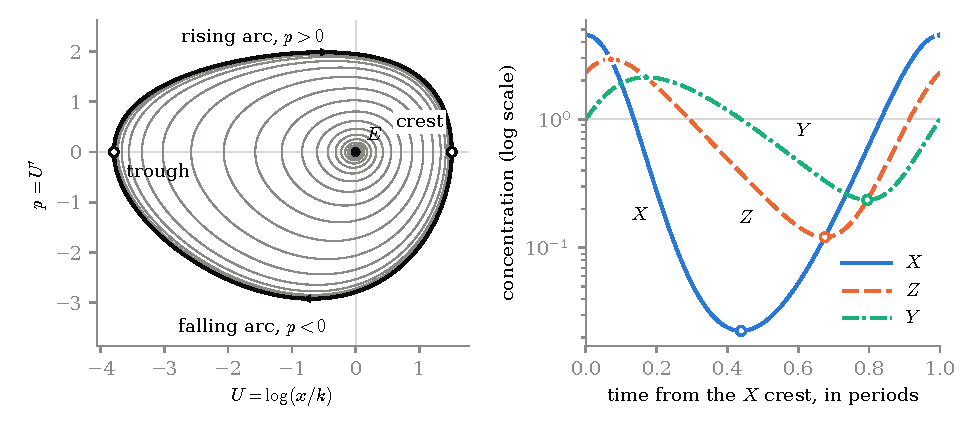
\includegraphics[width=\textwidth]{figures/fig_attractor.pdf}
\caption{Illustration at $\mu=1$, $\rho=1.3$, computed in floating point and not used in any proof. Left: projection to the $(U,p)$ plane of an orbit on the unstable manifold of $E$ (grey), which spirals clockwise out to the computed cycle (black); the projected cycle is strictly convex and star-shaped about $E$, and the rising arc ($p>0$) runs from trough to crest. Right: the three concentrations over one period on a logarithmic scale, starting at the $X$ crest; filled markers are maxima and open markers minima, in the order $X_{\max}$, $Z_{\max}$, $Y_{\max}$, $X_{\min}$, $Z_{\min}$, $Y_{\min}$ of Theorem~\ref{thm:six}.}\label{fig:attractor}
\end{figure}

\begin{theorem}[Finite-parameter obstruction, in original rates]\label{thm:main}
Fix any $a_0,b_0>0$. If \eqref{eq:physical} has more than one positive nonconstant periodic orbit at a finite growth rate $r_1>a_0+b_0$, then there is a rate
\[
a_0+b_0<r_*\le r_1
\]
at which a nonconstant positive cycle of physical least period $T_{\rm phys}$ has transverse Floquet multipliers
\begin{equation}\label{eq:physicalneutral}
1,\qquad \exp\{-(a_0+b_0)T_{\rm phys}\}.
\end{equation}
More generally, the number of cycles is constant along every compact parameter path in $\cP$ on which no cycle has an additional multiplier $+1$.
\end{theorem}
The multiplier $1$ in \eqref{eq:physicalneutral} is transverse to the autonomous tangent direction. Its existence is necessary for failure of uniqueness somewhere along the path; by itself it is not a counterexample. Theorem~\ref{thm:main} is proved in Section~\ref{sec:obstruction}.

\paragraph{What remains open.} Uniqueness is proved here in the region \eqref{eq:mainthreshold} and, by Lemma~\ref{lem:collar}, in a non-explicit right-hand neighbourhood of each Hopf point. For
\[
a_0+b_0<r_0<1000\,\frac{\max(a_0,b_0)^2}{\min(a_0,b_0)}
\]
outside those neighbourhoods the cycle count is not determined by the results of this paper. By Theorem~\ref{thm:mainattractor} the open statement is that $\avg\eta<\mu$ on every cycle; equivalent forms are collected in Section~\ref{sec:status}. Floating-point computation found no second cycle and no cycle with $\lambda_c\ge0$ (Section~\ref{sec:evidence}); that is evidence, not proof.

\subsection{A short route through the main argument}
For the principal conclusion, read the model and claim boundaries in this section,
the exact multiplier formula in Section~\ref{sec:adjoint}, the all-cycle geometric
framework in Sections~\ref{sec:support}--\ref{sec:geometry}, and the large-gain
theorem in Section~\ref{sec:largegain}. The attractor proof is in
Section~\ref{sec:attractor}; compactness and the neutral-cycle argument in
Sections~\ref{sec:compact}--\ref{sec:obstruction} explain why stability can force
uniqueness. The subsequent small-rate-ratio analysis, failed-certificate catalogue,
computational record and future programme are supplementary developments, not
additional assumptions of the large-gain theorem. The kurtosis inequality in
Theorem~\ref{thm:kurtosis} concerns general strictly convex potentials and can be
read as a reusable result independently of the oscillator application.

\subsection{Established inputs and self-contained scope}
Wilhelm and Heinrich introduced the model and analysed its local Hopf bifurcation \cite{WH95,WH96}. Smith proved that positive solutions are permanent, that the competitive Poincar\'e--Bendixson theorem applies, that above Hopf there are finitely many cycles, at least one of them orbitally asymptotically stable, and that every positive solution outside the stable manifold of the equilibrium converges to a cycle \cite[Theorems 1.1, 1.3 and 1.4]{Smith12}. Theorem 13 of Boros and Hofbauer summarises these results, includes stability through the critical value, and retains the cycle-count question \cite{BH23}. The mass-conserving extension in that paper is a different equation.

The sections below state at each use which of these inputs is required. Section~\ref{sec:attractor} proves dissipativity and the structure of the attractor directly and uses only classical planar and invariant-manifold theory. The remaining imported tools are Perron--Frobenius theory for a strictly positive evolution, smooth dependence of solutions on data, the implicit-function theorem, the Jordan curve theorem, the planar Poincar\'e--Bendixson theorem, local Hopf theory, and, for Theorem~\ref{thm:wedge} only, Eldering's invariant-graph persistence theorem \cite{Eldering13}. Appendix~\ref{app:hopf} reproduces the Hopf coefficient in a specified convention.

The full 1995 and 1996 articles of Wilhelm and Heinrich were not obtained; their publisher records and later primary accounts were inspected. No model-specific theorem is imported from a text that was not read. The classical results are listed with references at the point of use (Sections~\ref{sec:attractor} and~\ref{sec:wedge}) and are quoted in their standard form; their original sources were not re-read for this paper. For the revised local wedge result, Theorem~3.2 and Remark~3.3 of \cite{Eldering13} and the author's errata were inspected directly; Lemma~\ref{wed:lem:slowgraph} verifies their application. The Fenichel and Jones originals remain an access gap, but are not load-bearing for this revision.

\subsection{Positioning}
The literature search behind this subsection was bounded (citation graphs of \cite{Smith12,BH23,WH95,WH96}, preprint servers and keyword searches to 3 October 2026). It found no result that resolves or partially resolves the cycle count, and no published uniqueness theorem whose hypotheses the system satisfies. A bounded negative search does not establish priority. Table~\ref{tab:positioning} separates what is taken from the literature, what is a direct proof of a phenomenon known in a general theory, and what is advanced as new.

{\small
\begin{longtable}{p{0.36\textwidth}p{0.17\textwidth}p{0.39\textwidth}}
\caption{Positioning of the results. ``New'' means: not found in the sources inspected; priority is not otherwise established.}\label{tab:positioning}\\
\toprule
Result & Status & Relation to the literature\\
\midrule
\endfirsthead
\toprule
Result & Status & Relation to the literature\\
\midrule
\endhead
\bottomrule
\endfoot
Permanence; convergence to a cycle off the stable manifold of $E$; finitely many cycles, one stable; critical global stability & imported & \cite{Smith12}, \cite[Theorem 13]{BH23}\\
Supercritical Hopf bifurcation & imported, recomputed & \cite{WH96}; Appendix~\ref{app:hopf}\\
Linear-chain form of the distributed-delay logistic equation & known & \cite{Ruan06}; only local Hopf results are available for the strong kernel\\
\midrule
Real positive transverse multipliers (Proposition~\ref{prop:multipliers}) & direct proof & general competitive and cyclic feedback theory \cite{MPS90}\\
Injective planar projection of a cycle; one crest; order of extrema (Theorems~\ref{thm:geometry}, \ref{thm:six}) & direct proof & limit sets of competitive systems project injectively \cite{Hirsch82}; monotone cyclic feedback \cite{MPS90}\\
The attractor is a two-dimensional graph bounded by a cycle (part of Theorem~\ref{thm:attractor}) & direct proof for this model & analogues for scalar delay equations \cite{Walther95}; these allow several nested cycles\\
\midrule
Strict supporting planes between bounded orbits (Theorems~\ref{thm:support}, \ref{thm:twoorbit}) & new & mechanism related to convex carrying simplices \cite{Baigent13}\\
Convexity and $C^1$ regularity of the attractor graph; planar divergence $\eta-\mu$; parameter-wise criterion (Theorem~\ref{thm:attractor}, Corollary~\ref{cor:criterion}) & new & ---\\
Convex star-shaped projections; exact formulas \eqref{eq:mainformula}; scalar Riccati reduction (Theorem~\ref{thm:gauges}, Proposition~\ref{prop:kappa}) & new & the gauges are the angular and curvature functions used in planar Dulac criteria \cite{GG21}, whose hypotheses fail here\\
Weak-adjoint zero order; strong-stable supporting planes (Theorems~\ref{thm:twelve}, \ref{thm:dualsupport}) & new & uses the sign structure of \cite{MPS90}\\
Uniform compactness of cycle families; neutral-cycle obstruction (Theorems~\ref{thm:compact}, \ref{thm:neutral}) & new & ---\\
Uniqueness for large gain with an explicit threshold (Theorem~\ref{thm:largegain}) & new & large-parameter step of the proof of Jones' conjecture \cite{Xie93} is the analogue\\
Kurtosis bound for convex potentials; local wedge theorem (Theorems~\ref{thm:kurtosis}, \ref{thm:wedge}) & proposed new results & slow-graph property derived in Lemma~\ref{wed:lem:slowgraph} using \cite{Eldering13}\\
Failure of specific certificates (Section~\ref{sec:negative}) & new negative results & hypotheses of \cite{Massera54,Zhang86,SmithHL86,SV10,GG21} tested and found to fail\\
\end{longtable}}

\paragraph{Comparison with convex carrying simplices.}
Baigent's discrete-time criterion \cite[Section~4, Theorem~6.1]{Baigent19}
assumes a face-preserving competitive Kolmogorov diffeomorphism and controlled
images of planes. Mierczy\'nski \cite[Sections~2--3]{Mierczynski20} obtains
regularity from convexity for carrying simplices under hypotheses including
forward and backward invariance of coordinate faces. Those hypotheses do not
hold for the Wilhelm--Heinrich flow in its physical coordinates: at $y=0,z>0$
the derivative $y'=a_0z$ points into the interior, and at $z=0,x>0$ one has
$z'=b_0x>0$. Thus these theorems do not directly supply the present graph result.
The specific contributions here are the strict supporting inequality between
bounded entire trajectories, its positive-adjoint supporting planes, the graph
in logarithmic coordinates, and the reduced divergence formula. This comparison
is not a claim that a different transformation or another theorem cannot apply.
In particular, the full text of Li's 1981 third-order uniqueness work was not
obtained, so its applicability and any resulting priority implications remain
unresolved. Here ``convex graph'' always means a graph of a convex function,
not a convex subset of $\R^3$.

\subsection{Notation}
Table~\ref{tab:notation} lists the symbols used throughout. Sections that need further symbols introduce them in their first paragraph.

{\small
\begin{longtable}{p{0.42\textwidth}p{0.52\textwidth}}
\caption{Global notation.}\label{tab:notation}\\
\toprule
Symbol & Meaning\\
\midrule
\endfirsthead
\toprule
Symbol & Meaning\\
\midrule
\endhead
\bottomrule
\endfoot
$\mu,\ k,\ A,\ \lambda,\ \kH,\ \rho$ & parameters \eqref{eq:parameters}; $\delta=k-\kH$; $\cP$ the oscillatory domain\\
$t$, $\tau=\sqrt\mu\,t$ & fast time; frequency-one time\\
$(U,p,y)$, $x=ke^U$, $E$ & state \eqref{eq:logsystem}; equilibrium $(0,0,k)$\\
$X,Y,Z$; $\ell=\lambda-p$ & chemical variables \eqref{eq:filters}; $\ell=\lambda Y>0$\\
$T$, $\avg{\cdot}$ & least period of a cycle; time average over it\\
$\eta,\zeta$; $\gamma=1+\avg\eta$ & positive adjoint ratios \eqref{eq:ratios}; principal adjoint exponent\\
$m_s<m_t$; $\lambda_c=\avg\eta-\mu$ & transverse Floquet multipliers; weak exponent\\
$\gamma_E,\eta_E,\zeta_E$ & adjoint data of the equilibrium (Corollary~\ref{cor:cones})\\
$K,\ W,\ \LamE$ & convexity gauges \eqref{eq:positiveK}, \eqref{eq:curvature}, \eqref{eq:LambdaE}\\
$\psiU(U)=Ue^U-e^U+1$, $\Rem(d)=e^d-1-d$ & convex remainders\\
$\Sg=p^2-Up'$, $\Xg=p'^2-pp''$ & star gauge; convexity gauge of the projected cycle\\
$\kappa=K/\Sg$; $\etaz$ & gauge ratio; explicit state function with mean $\mu$ (Theorem~\ref{thm:gauges})\\
$M$; $M_{(U,z)}$ & crest-return derivative in $(U,y)$; in $(U,z)$, $z=y/k$\\
$C$; $C_\pm$ & compound matrix \eqref{eq:compound}; cones \eqref{eq:cones}\\
$e_s=(a,-b,-c)$; $\mathfrak r=b/a$, $\mathfrak s=c/a$; $\Psi$ & strong-stable Floquet vector and ratios; weak adjoint\\
$\cA$, $\Dom$, $\pi$, $\Dsc$, $h$ & attractor, chemical domain, projection to $(U,p)$, $\pi(\cA)$, graph function\\
$D$; $\Dt$ & $\mathrm d/\mathrm dt$ in operator identities; derivative of a state function along the flow\\
\end{longtable}}

% s02_adjoint.tex -- positive adjoint and exact transverse exponent.
% Exported labels: sec:adjoint eq:adjointmatrices eq:ratios eq:projective eq:etaminbasic prop:multipliers
% eq:multipliers eq:exponent prop:factor eq:orthogonality eq:tangent eq:factorisation lem:projectivebounds
% eq:gainprimitive.  Internal labels carry the prefix adj:.
\section{A positive adjoint and the exact transverse exponent}\label{sec:adjoint}
Besides the global notation, this section introduces the Jacobian $J$, the adjoint matrix $B$, the signature matrix $S$, the positive adjoint solution $\mathbf H=(H_1,H_2,H_3)^{\mathsf T}$, the normal vector $n$ and the tangent pairing $O$. They keep these meanings in later sections.

\subsection{Projective equations}\label{adj:sec:projective}
Along any cycle of \eqref{eq:logsystem},
\begin{equation}\label{eq:adjointmatrices}
J=\begin{pmatrix}0&1&0\\0&-\mu&-1\\x&0&-1\end{pmatrix},\qquad
B=-SJ^{\mathsf T}S=\begin{pmatrix}0&0&x\\1&\mu&0\\0&1&1\end{pmatrix},\qquad
S=\diag(1,-1,-1).
\end{equation}
The evolution of $\mathbf H'=B\mathbf H$ is strictly positive over each positive time interval: every pair of coordinates is connected through the positive cyclic links, including $x(t)>0$. Its period matrix therefore has a simple strictly dominant positive Perron eigenvalue and a positive eigenvector. Propagating this vector gives a positive Floquet solution $\mathbf H$ whose component ratios are periodic. Define
\begin{equation}\label{eq:ratios}
\eta=H_2/H_3>0,\qquad \zeta=H_1/H_3>0.
\end{equation}
Direct differentiation gives
\begin{equation}\label{eq:projective}
\eta'=\zeta+(\mu-1)\eta-\eta^2,\qquad
\zeta'=x-(1+\eta)\zeta.
\end{equation}
At a minimum of $\eta$, the first equation implies
\begin{equation}\label{eq:etaminbasic}
\eta>\max(0,\mu-1).
\end{equation}
Since $H_3'=(1+\eta)H_3$, the principal adjoint exponent is $\gamma=1+\avg\eta>1$.

\begin{proposition}[Positive transverse multipliers]\label{prop:multipliers}
The two transverse multipliers satisfy
\begin{equation}\label{eq:multipliers}
0<m_s<m_t,\qquad m_s<1,\qquad m_sm_t=e^{-AT},
\end{equation}
and, exactly,
\begin{equation}\label{eq:exponent}
m_s=e^{-(1+\avg\eta)T},\qquad
m_t=e^{(\avg\eta-\mu)T},\qquad
\lambda_c:=T^{-1}\log m_t=\avg\eta-\mu.
\end{equation}
Thus hyperbolic orbital attraction is equivalent to $\avg\eta<\mu$.
\end{proposition}
\begin{proof}
The adjoint monodromy is sign-conjugate to the inverse transpose of the original monodromy. The reciprocal of its Perron eigenvalue is an original multiplier $m_s$, smaller in modulus than either remaining multiplier. One remaining multiplier is the autonomous tangent multiplier $1$. Since $\tr J=-A$, Liouville's identity makes the product of the transverse multipliers $e^{-AT}>0$. The remaining multiplier is real and positive, and the formulas follow. The argument allows a repeated ambient multiplier $1$; the two transverse multipliers themselves are distinct.
\end{proof}
When $\avg\eta=\mu$, nonlinear orbital stability is undecided by this criterion. An ambient Jordan block at the unit multiplier is not excluded.

\subsection{Tangent orthogonality and factorisation}\label{adj:sec:factor}
\begin{proposition}\label{prop:factor}
Along every cycle,
\begin{equation}\label{eq:orthogonality}
\zeta p-\eta p'-(x-y)=0,
\end{equation}
so its scalar tangent satisfies
\begin{equation}\label{eq:tangent}
p''=(\eta-\mu)p'-\zeta p.
\end{equation}
With the displayed periodic coefficients, the scalar variational operator factors as
\begin{equation}\label{eq:factorisation}
D^3+AD^2+\mu D+x=(D+1+\eta)\bigl[D^2+(\mu-\eta)D+\zeta\bigr].
\end{equation}
\end{proposition}
\begin{proof}
Put $n=(\zeta,-\eta,-1)^{\mathsf T}$. Equations \eqref{eq:projective} give
\[
n'+J^{\mathsf T}n+(1+\eta)n=0.
\]
Pairing with the tangent gives $O'+(1+\eta)O=0$, where $O$ is the left side of \eqref{eq:orthogonality}. Its only periodic solution is zero because $1+\eta>1$. Also $p''=-\mu p'-x+y$, proving \eqref{eq:tangent}. Expanding \eqref{eq:factorisation}, its $D$ coefficient is $\zeta-\eta'+(1+\eta)(\mu-\eta)=\mu$, and its constant coefficient is $\zeta'+(1+\eta)\zeta=x$. The $D^2$ coefficient is $A$.
\end{proof}

\begin{lemma}[Explicit bounds independent of the period]\label{lem:projectivebounds}
Suppose $0<x_-\le x(t)\le x_+$. Set
\begin{align*}
\eta_+&=\frac{\mu-1+\sqrt{(\mu-1)^2+4x_+}}2,&
\zeta_-&=\frac{x_-}{1+\eta_+},\\
\eta_-&=\frac{\mu-1+\sqrt{(\mu-1)^2+4\zeta_-}}2,&
\zeta_+&=\frac{x_+}{1+\eta_-}.
\end{align*}
Then $\eta_-\le\eta\le\eta_+$ and $\zeta_-\le\zeta\le\zeta_+$.
\end{lemma}
\begin{proof}
At a maximum of $\zeta$, its equation gives $\zeta\le x_+$. At a maximum of $\eta$, the first equation gives $\eta(\eta+1-\mu)=\zeta\le x_+$, yielding $\eta_+$. At a minimum of $\zeta$ it gives $\zeta\ge x_-/(1+\eta_+)$. The corresponding minimum equation for $\eta$ gives $\eta_-$, and using that bound at a maximum of $\zeta$ gives $\zeta_+$. The relevant quadratic has a unique positive root in the range \eqref{eq:etaminbasic}.
\end{proof}

An exact primitive is
\begin{equation}\label{eq:gainprimitive}
(\zeta+\eta+\eta^2/2)'=x-f_\mu(\eta),\qquad
f_\mu(s)=s(s+1)(s+1-\mu).
\end{equation}
Since $\avg x=k$, it follows that $k=\avg{f_\mu(\eta)}$. A constant $\eta$ would force $\zeta$ and then $x$ constant, so $\eta$ is nonconstant on a nonconstant cycle. This identity constrains moments of $\eta$; by itself it does not determine the sign of $\avg\eta-\mu$.

% s03_support.tex -- strict supporting planes for cycles.
% Exported labels: sec:support thm:support eq:delta eq:supportidentity cor:cones eq:positiveK
% eq:equilibriumreverse eq:LambdaE eq:cones lem:curvature eq:curvature.  Internal labels carry the prefix sup:.
\section{Strict supporting planes for entire solutions}\label{sec:support}
Local symbols of this section: $z_1,z_2$ denote solutions $z_j=(U_j,p_j,y_j)$ of \eqref{eq:logsystem}, with $x_j=ke^{U_j}$ and $J_1$ the Jacobian \eqref{eq:adjointmatrices} along $z_1$; $\Delta$ is the gap function \eqref{eq:delta}; $r=(U,p,y-k)$ is a cycle point measured from $E$.

\begin{theorem}[Exact two-solution comparison]\label{thm:support}
Let $z_1=(U_1,p_1,y_1)$ be a cycle or the equilibrium of \eqref{eq:logsystem}, with its positive adjoint ratios $\eta,\zeta$. Let $z_2$ be a distinct entire solution at the same parameters, bounded in logarithmic coordinates for all real times. Then
\begin{equation}\label{eq:delta}
\Delta=\zeta(U_2-U_1)-\eta(p_2-p_1)-(y_2-y_1)
\end{equation}
satisfies
\begin{equation}\label{eq:supportidentity}
\Delta'+(1+\eta)\Delta=-x_1\,\Rem(U_2-U_1),\qquad \Rem(d):=e^d-1-d,
\end{equation}
and $\Delta(t)<0$ for every $t$. Distinct phases of the same cycle are allowed.
\end{theorem}
\begin{proof}
The difference of the vector fields equals $J_1(z_2-z_1)$ plus
$(0,0,x_2-x_1-x_1(U_2-U_1))^{\mathsf T}=(0,0,x_1\Rem(U_2-U_1))^{\mathsf T}$. Pair with the normal $n$ from Proposition~\ref{prop:factor}. This proves the identity without truncating the exponential. Its bounded entire solution is
\[
\Delta(t)=-\int_{-\infty}^t
 e^{-\int_s^t(1+\eta(v))\,\mathrm dv}\,
 x_1(s)\,\Rem\bigl(U_2(s)-U_1(s)\bigr)\,\mathrm ds.
\]
The exponential kernel decays at least as $e^{-(t-s)}$ and all remaining factors are bounded. Strict convexity makes $\Rem$ nonnegative, with $\Rem(d)=0$ only at $d=0$. If the integrand vanished throughout a past half-line, the two $U$ components would coincide there; differentiating the equations would identify $p,y$ and then both solutions. Thus the integral is strictly negative.
\end{proof}
The hypothesis of an entire solution bounded in log coordinates is satisfied by every positive cycle and by the positive equilibrium. It is not assumed for arbitrary forward trajectories. Section~\ref{sec:attractor} (Theorem~\ref{thm:twoorbit}) extends the comparison to arbitrary pairs of distinct log-bounded entire orbits.

\begin{corollary}[Two different equilibrium comparisons]\label{cor:cones}
Along every cycle in $\cP$,
\begin{equation}\label{eq:positiveK}
K:=\zeta U-\eta p-y+k>0,\qquad
K'+(1+\eta)K=xU-x+k=k\,\psiU(U),
\end{equation}
where $\psiU(U):=Ue^U-e^U+1$. Let $\gamma_E>A$ be the unique root of
\[
k=\gamma_E(\gamma_E-1)(\gamma_E-\mu),
\]
and set $\eta_E=\gamma_E-1$, $\zeta_E=(\gamma_E-1)(\gamma_E-\mu)$. Then the linear gauge
\begin{equation}\label{eq:LambdaE}
\LamE:=(y-k)-\zeta_EU+\eta_Ep
\qquad\text{satisfies}\qquad
\LamE>0,\qquad \LamE'=-\gamma_E\LamE+k\,\Rem(U)
\end{equation}
along every cycle; that is,
\begin{equation}\label{eq:equilibriumreverse}
\zeta_EU-\eta_Ep-y+k<0.
\end{equation}
Consequently no cycle point $r=(U,p,y-k)$ belongs to either closed cone
\begin{equation}\label{eq:cones}
C_+=\{U\ge0,\ p\le0,\ y-k\le0\},\qquad C_-=-C_+.
\end{equation}
\end{corollary}
\begin{proof}
Use the cycle as the base and the equilibrium as the second solution to obtain $K>0$. Differentiation gives its primitive; equivalently, in this case $\Delta=-K$ and $x\,\Rem(-U)=k\,\psiU(U)$ in \eqref{eq:supportidentity}. Reversing the roles gives \eqref{eq:equilibriumreverse}; the constant ratios follow by solving the positive equilibrium adjoint eigenvector equation $B(\zeta_E,\eta_E,1)^{\mathsf T}=\gamma_E(\zeta_E,\eta_E,1)^{\mathsf T}$ at $x=k$. With the equilibrium as base, $\Delta=-\LamE$, $x_1=k$ and $1+\eta_E=\gamma_E$, so \eqref{eq:supportidentity} is the differential relation in \eqref{eq:LambdaE}. The left side of \eqref{eq:equilibriumreverse}, namely $-\LamE$, is nonnegative on $C_+$, whereas $K$ is nonpositive on $C_-$. These contradictions exclude both cones, including their boundaries. The two signs require two distinct choices of base; one does not follow by reversing \eqref{eq:positiveK} alone.
\end{proof}

\begin{lemma}[Strict supporting curvature]\label{lem:curvature}
The function
\begin{equation}\label{eq:curvature}
W=\zeta'p-\eta'p'
\end{equation}
satisfies $W'+(1+\eta)W=xp^2$, and $W>0$ at every phase of a nonconstant cycle.
\end{lemma}
\begin{proof}
Differentiate using \eqref{eq:projective} and \eqref{eq:orthogonality}. The positive periodic convolution of $xp^2$ gives $W$. Its source is nonnegative and not identically zero, proving strict positivity. Off the constraint $O=0$, the polynomial residual of the differential identity is $-\eta'O$; the identity therefore holds along cycles and not for arbitrary independent values of $(U,p,y,\eta,\zeta)$.
\end{proof}

% s04_geometry.tex -- one crest, six extrema, crest map.
% Exported labels: sec:geometry thm:geometry eq:crestidentities thm:six eq:six cor:orderedcrests eq:crestorder
% prop:crestmap eq:compound eq:determinant.  Internal labels carry the prefix geo:.
\section{Every cycle has one ordered sequence of six extrema}\label{sec:geometry}
Local symbols of this section: the subscripts $o$ and $i$ mark an outer and an inner projected cycle; $(\xi_U,\xi_y)$ is a variation within the crest section $\{p=0\}$ in the coordinates $(U,y)$; $w$ is the sign-conjugated wedge of the tangent and a variation; $z=y/k$ is the rescaled section coordinate, equal to the concentration $Z$ of \eqref{eq:change}.

\begin{theorem}[Planar embedding and unimodality]\label{thm:geometry}
Every nonconstant positive cycle has a regular injective projection into $(U,p)$. It is a clockwise Jordan curve enclosing $(0,0)$. In one least period $U$ has one nondegenerate maximum and minimum, and $p$ has one positive nondegenerate maximum and one negative nondegenerate minimum. Projections of distinct cycles at the same parameters are disjoint and nested.
\end{theorem}
\begin{proof}
If two distinct periodic points had equal $(U,p)$, Theorem~\ref{thm:support} with the first as base would require the second to have larger $y$. Reversing the bases requires the opposite inequality. This excludes both a crossing between different cycles and a self-crossing of one projected cycle.

If the projected tangent vanished, $p=p'=0$. Equation~\eqref{eq:orthogonality} gives $x=y$, while $p'=k-y$ gives $x=y=k$. This is the equilibrium and cannot lie on a nonconstant cycle. The projection is therefore a regular embedded circle.

At a zero of $p$, \eqref{eq:orthogonality} gives
\begin{equation}\label{eq:crestidentities}
x-k=(1+\eta)(y-k),\qquad x-y=\eta(y-k),\qquad p'=k-y.
\end{equation}
No such zero has $U=0$. Every positive-$U$ axis crossing is downward; every negative-$U$ crossing is upward. The identity $\avg x=k$ forces $U$ to have both signs. The global maximum of $U$ is consequently a downward positive-ray crossing. The winding number of a Jordan curve about a point not on it is $0$ or $\pm1$. All crossings of that ray are transverse with the same sign, so there is exactly one and the winding number is $-1$. The negative ray likewise has exactly one crossing. Thus $p$ has exactly two simple zeros.

Between them $p$ has a fixed sign. At $p'=0$, \eqref{eq:tangent} gives $p''=-\zeta p$. On the positive half-cycle every critical point is a strict maximum, and on the negative half-cycle every critical point is a strict minimum. There is exactly one of each: two strict maxima on the same interval would require an intervening critical point that is not a strict maximum. Finally, disjoint Jordan curves that both enclose the origin have nested interiors.
\end{proof}

\begin{theorem}[Chemical phase order in the original labelling]\label{thm:six}
All three physical concentrations in \eqref{eq:filters} have exactly one maximum and one minimum in a least period, and all six extrema are nondegenerate. Starting at the minimum of $X$, their strict cyclic order is
\begin{equation}\label{eq:six}
X_{\min}\;<\;Z_{\min}\;<\;Y_{\min}\;<\;
X_{\max}\;<\;Z_{\max}\;<\;Y_{\max}\;<\;X_{\min}+T,
\end{equation}
where inequalities refer to event times. At an $X$ crest, $X>Z>1$ and $Y=1$; at its trough, $X<Z<1$ and $Y=1$.
\end{theorem}
\begin{proof}
Extrema of $X$ coincide with zeros of $p$ and are nondegenerate by \eqref{eq:crestidentities}. Since $Y=1-p/\lambda$, its extrema are the two critical points of $p$ identified above, and $Y''=\zeta p/\lambda$ there.

For the intermediate filter, $y'=x-y$ and, at a zero of $y'$,
\[
y''=xp.
\]
At the $X$ trough, \eqref{eq:crestidentities} gives $y'<0$; at the next $X$ crest it gives $y'>0$. Throughout that interval $p>0$, so every zero of $y'$ is a strict upward crossing. There is exactly one, the $Z$ minimum. At the positive maximum of $p$, \eqref{eq:orthogonality} gives $y'=\zeta p>0$, so the $Z$ minimum precedes the $Y$ minimum. On the negative half-cycle all zeros of $y'$ are strict downward crossings. Its unique zero, the $Z$ maximum, precedes the negative minimum of $p$, since $y'=\zeta p<0$ there. This proves \eqref{eq:six}. Positivity of $x,\zeta$ gives nondegeneracy. The concentration inequalities are exactly \eqref{eq:crestidentities} divided by $k$.
\end{proof}

\begin{corollary}[Ordered crests of nested cycles]\label{cor:orderedcrests}
Let an outer projected cycle and an inner projected cycle have positive-axis crests $(U_o,y_o)$ and $(U_i,y_i)$. Then $U_o>U_i$ and $y_o>y_i$. More precisely,
\begin{equation}\label{eq:crestorder}
\zeta_i(U_o-U_i)<y_o-y_i<\zeta_o(U_o-U_i).
\end{equation}
In particular $\zeta_o>\zeta_i$ at these respective crests. At the negative-axis trough the outer cycle has both smaller $U$ and smaller $y$.
\end{corollary}
\begin{proof}
Nesting and the unique ray crossing give the order of $U$. Apply the strict supporting inequalities in both directions to the two phase-fixed crest points, where $p=0$. They give \eqref{eq:crestorder}. The same two inequalities with negative $U_o-U_i$ give the trough statement.
\end{proof}

\begin{proposition}[Positive crest derivative and strong area contraction]\label{prop:crestmap}
The local first downward return on $p=0$ at a cycle crest, expressed in the section coordinates $(U,y)$, has an entrywise positive derivative $M$. Its eigenvalues are $m_s,m_t$ from Proposition~\ref{prop:multipliers}, and
\begin{equation}\label{eq:determinant}
\det M=e^{-AT}<e^{-4\pi},\qquad T>\frac{2\pi}{\sqrt\mu}.
\end{equation}
In the section coordinates $(U,z)$, $z=y/k$, the same derivative is represented by
\begin{equation}\label{geo:eq:similarity}
M_{(U,z)}=\diag(1,1/k)\,M\,\diag(1,k)
=\begin{pmatrix}M_{11}&kM_{12}\\ M_{21}/k&M_{22}\end{pmatrix}.
\end{equation}
The matrices $M$ and $M_{(U,z)}$ have the same eigenvalues, the same determinant and the same sign pattern. Their individual entries depend on the choice of section coordinates, and so does any componentwise inequality tested on a vector: a test vector $\xi$ for $M$ corresponds to $\diag(1,1/k)\,\xi$ for $M_{(U,z)}$.
\end{proposition}
\begin{proof}
At a crest $x>y>k$. For a section variation $(\xi_U,0,\xi_y)$ the sign-conjugated wedge of the tangent and variation is
\[
w=\bigl((y-k)\xi_U,\ (x-y)\xi_U,\ (y-k)\xi_y\bigr)^{\mathsf T}.
\]
It evolves by
\begin{equation}\label{eq:compound}
w'=Cw,\qquad C=\begin{pmatrix}-\mu&1&0\\0&-1&1\\x&0&-A\end{pmatrix}.
\end{equation}
Each nonzero nonnegative coordinate variation starts a nonzero nonnegative wedge, which becomes strictly positive. At the return crest its first and third entries recover $\xi_U,\xi_y$ by division by $y-k>0$. The event-time correction adds a multiple of the tangent and does not alter this wedge. This proves entrywise positivity of $M$.

Multiply \eqref{eq:scalar} by $U'$ and integrate to get $\int_0^T(p')^2\dd=\mu\int_0^T p^2\dd$. The periodic Wirtinger inequality for the mean-zero function $p$ gives $T\ge2\pi/\sqrt\mu$. Equality would force $U=c_0+c_1\cos(\sqrt\mu t+\theta)$, $c_1>0$. Substitution cancels $U'''+\mu U'$ and would make its exponential affine in the cosine, which strict convexity excludes. Thus the period inequality is strict. Liouville's identity gives $\det M=e^{-AT}$, and $AT>2\pi(\sqrt\mu+1/\sqrt\mu)\ge4\pi$.

A variation $(\xi_U,\xi_y)$ in the coordinates $(U,y)$ is the variation $(\xi_U,\xi_y/k)=\diag(1,1/k)(\xi_U,\xi_y)^{\mathsf T}$ in the coordinates $(U,z)$. Conjugating $M$ by this positive diagonal matrix gives \eqref{geo:eq:similarity}; a similarity preserves eigenvalues and determinant, and a positive diagonal one preserves the sign of every entry.
\end{proof}
Small determinant does not imply contraction of every direction. In particular, it does not exclude $m_t\ge1$.

\section{Convex star-shaped projections and exact formulas for the weak exponent}\label{sec:gauges}
This section proves that the projection of every cycle to the $(U,p)$ plane is strictly star-shaped about the origin and strictly convex. The two positive functions that express these properties satisfy linear equations driven by the convexity gauges $K$ and $W$, and averaging those equations gives exact formulas for the weak exponent $\lambda_c$. The remaining subsections record the consequences: a reduction of the adjoint ratios to one scalar Riccati equation, a polar form, a comparison of nested cycles, sign-definite integrals, exact moment identities, a pairing with the strong-stable Floquet solution, and injectivity of the Gauss map. Besides the identities of Section~\ref{sec:adjoint}, the proofs use Theorems~\ref{thm:support} and~\ref{thm:geometry}, Corollary~\ref{cor:cones} and Lemma~\ref{lem:curvature}; Proposition~\ref{prop:strongidentity} also uses Lemma~\ref{lem:strongstable} and the compound system \eqref{eq:compound}. No proof uses the stability of a cycle, the number of cycles, or any property of $(\mu,k)$ other than the existence of a cycle. Floating-point evidence for the formulas is reported in Section~\ref{sec:evidence}; it plays no part in the proofs.

\paragraph{Local notation.}
A cycle with least period $T$ is fixed unless two cycles are named. By Theorem~\ref{thm:geometry}, $p$ has exactly two zeros in a period, both simple: the \emph{trough}, at a time $t_a$, where $U=U_{\min}<0$, and the \emph{crest}, at the time $t_b\in(t_a,t_a+T)$, where $U=U_{\max}>0$. The \emph{rising arc} is $(t_a,t_b)$, on which $p>0$; the \emph{falling arc} is $(t_b,t_a+T)$, on which $p<0$. We write $q=(U,p)$ for the projected point, $v\wedge w=v_1w_2-v_2w_1$ for planar vectors, and
\[
L_2=D^2+(\mu-\eta)D+\zeta
\]
for the second-order factor in \eqref{eq:factorisation}. Besides the global symbols $\Sg$, $\Xg$, $\kappa=K/\Sg$ and $\etaz$, this section uses: $\zeta_0=\Xg/\Sg$ and $\eta_1$ (Theorem~\ref{thm:gauges}); $\Sg_c=p^2-(U+c)p'$ for a shift $c\ge0$; polar coordinates $(U,p)=r(\cos\theta,\sin\theta)$ with $s=(y-k)/r$ and $\sigma=\Sg/r^2$; for two nested cycles $R_i(\theta)$, $s_i(\theta)$, $\sigma_i(\theta)$, $i=1,2$; the chain ratios $r_1=x/y$, $r_2=y/\ell$; the polynomials $f_\mu(s)=s(s+1)(s+1-\mu)$ of \eqref{eq:gainprimitive}, $\chi(s)=s(s-1)(s-\mu)$ and $G_\mu(s)=\tfrac32s^2+(2-\mu)s$; the operator $\mathcal L[w]=w''+(3w+2-\mu)w'+f_\mu(w)$; the variable $\omega=\zeta+\eta+\eta^2/2$ (in Proposition~\ref{prop:gaussmap} only); and a hat for the periodic part of a strong-stable Floquet component, $\hat a=e^{\gamma t}a$. The letters $r_1,r_2$ denote chain ratios and are unrelated to the polar radius $r$.

\subsection{Two positive gauges}
\begin{lemma}[Wronskian gauge identity]\label{gau:wronskian}
Let $f,g$ be $C^2$ functions of $t$ along a cycle and put $V_{f,g}=fg'-f'g$. Then
\begin{equation}\label{gau:wronskianeq}
V_{f,g}'=(\eta-\mu)V_{f,g}+f\,L_2[g]-g\,L_2[f].
\end{equation}
Moreover
\begin{equation}\label{gau:Ltwovalues}
L_2[1]=\zeta,\qquad L_2[U]=K,\qquad L_2[p]=0,\qquad L_2[-p']=W .
\end{equation}
\end{lemma}
\begin{proof}
$V_{f,g}'=fg''-f''g$. Write $g''=L_2[g]-(\mu-\eta)g'-\zeta g$ and the same for $f$; the terms $\zeta fg$ cancel and
\[
fg''-f''g=f\,L_2[g]-g\,L_2[f]+(\eta-\mu)(fg'-f'g).
\]
The first value in \eqref{gau:Ltwovalues} is immediate. Since $U'=p$ and $p'=k-\mu p-y$,
\[
L_2[U]=p'+(\mu-\eta)p+\zeta U=k-y-\eta p+\zeta U=K .
\]
The identity $L_2[p]=0$ is \eqref{eq:tangent}. Differentiating it gives $L_2[p']-\eta'p'+\zeta'p=0$, that is, $L_2[-p']=\zeta'p-\eta'p'=W$ by \eqref{eq:curvature}.
\end{proof}

\begin{theorem}[Star gauge, convexity gauge and exact exponent]\label{thm:gauges}
On every cycle of \eqref{eq:logsystem} the following hold.
\begin{enumerate}[label=(\roman*)]
\item \emph{Positivity.} The functions $\Sg=p^2-Up'$ and $\Xg=p'^2-pp''$ are positive at every phase, and
\begin{equation}\label{eq:gaugeodes}
\Sg'=(\eta-\mu)\Sg+pK,\qquad \Xg'=(\eta-\mu)\Xg+pW .
\end{equation}
Both are functions of the state: with $p'=k-\mu p-y$, one has $\Sg=p^2-Up'$ and $\Xg=p'(k-y)+p(x-y)$.
\item \emph{Star shape.} The projected cycle does not pass through the origin, its polar angle satisfies
\[
\frac{\mathrm d}{\mathrm dt}\arg(U+ip)=-\frac{\Sg}{U^2+p^2}<0
\]
and decreases by exactly $2\pi$ in one period. Every ray from the origin meets the projected cycle in exactly one point, and transversally.
\item \emph{Strict convexity.} The signed curvature of the projected cycle is $-\Xg/(p^2+p'^2)^{3/2}<0$, and its tangent angle $\arg(p+ip')$ decreases by exactly $2\pi$ in one period. Every tangent line is a strict supporting line: for every $t_1$ and every point $q\ne q(t_1)$ of the closed region bounded by the projected cycle, in particular for $q=q(t)$ with $t\not\equiv t_1\pmod T$ and for $q=(0,0)$,
\begin{equation}\label{gau:supportline}
\bigl(p(t_1),p'(t_1)\bigr)\wedge\bigl(q-q(t_1)\bigr)<0 .
\end{equation}
That region is the convex hull of the projected cycle.
\item \emph{Exact exponent.} With $\oint f\,\mathrm dU=\int_0^Tf\,p\dd$,
\begin{equation}\label{eq:exactexponent}
\lambda_c=-\avg{\frac{pK}{\Sg}}=-\avg{\frac{pW}{\Xg}},\qquad
\lambda_cT=-\oint\frac{K}{\Sg}\,\mathrm dU=-\oint\frac{W}{\Xg}\,\mathrm dU .
\end{equation}
More generally, for every $\vartheta\in[0,1]$,
\begin{equation}\label{gau:mixedexponent}
\lambda_c=-\avg{\frac{p\,[(1-\vartheta)K+\vartheta W]}{(1-\vartheta)\Sg+\vartheta\,\Xg}} .
\end{equation}
\item \emph{Shifted centres.} For every $c$ with $0\le c<|U_{\min}|$ the function $\Sg_c=p^2-(U+c)p'$ is positive at every phase,
\begin{equation}\label{gau:shifted}
\Sg_c'=(\eta-\mu)\Sg_c+p\,(K+c\,\zeta),\qquad
\lambda_c=-\avg{\frac{p\,(K+c\,\zeta)}{\Sg_c}},
\end{equation}
and the conclusions of \textup{(ii)} hold for rays from $(-c,0)$.
\item \emph{Explicit comparison functions.} The state functions
\begin{equation}\label{gau:etazero}
\etaz=\frac{U(x-y)-p(y-k)}{\Sg},\qquad
\eta_1=\frac{x\Sg+k\psiU(U)\,p'}{\Xg}-1
\end{equation}
satisfy $(\log\Sg)'=\etaz-\mu$ and $(\log\Xg)'=\eta_1-\mu$, hence $\avg{\etaz}=\avg{\eta_1}=\mu$, and
\begin{equation}\label{gau:etadifference}
\eta-\etaz=-\frac{pK}{\Sg},\qquad \eta-\eta_1=-\frac{pW}{\Xg}.
\end{equation}
Consequently $\eta<\min(\etaz,\eta_1)$ on the rising arc, $\eta>\max(\etaz,\eta_1)$ on the falling arc, $\eta=\etaz=\eta_1$ at the crest and at the trough, and $\lambda_c=\avg{\eta-\etaz}=\avg{\eta-\eta_1}$.
\end{enumerate}
\end{theorem}
\begin{proof}
\emph{The gauge equations.} In Lemma~\ref{gau:wronskian} take $f=p$, so that $L_2[f]=0$. For $g=U$ one has $V_{p,U}=pU'-p'U=\Sg$ and $L_2[U]=K$. For $g=-p'$ one has $V_{p,-p'}=p'^2-pp''=\Xg$ and $L_2[-p']=W$. For $g=U+c$ one has $V_{p,U+c}=\Sg-cp'=\Sg_c$ and $L_2[U+c]=K+c\zeta$. Equation \eqref{gau:wronskianeq} gives \eqref{eq:gaugeodes} and the first equation in \eqref{gau:shifted}. Since $p''=-\mu p'-(x-y)$ and $p'+\mu p=k-y$,
\[
\Xg=p'^2+\mu pp'+p(x-y)=p'(k-y)+p(x-y).
\]

\emph{Values at the zeros of $p$.} At a zero of $p$, \eqref{eq:crestidentities} gives $x-k=(1+\eta)(y-k)$ and $p'=k-y$. If $U=0$ there, then $x=k$, hence $y=k$ and $p'=0$, and the point would be the equilibrium. Thus $U\ne0$, and $y-k$ has the sign of $x-k$, which is the sign of $U$. At $t_a$ and $t_b$ therefore
\[
\Sg=-Up'=U(y-k)>0,\qquad \Xg=p'^2=(y-k)^2>0,\qquad \Sg_c=(U+c)(y-k).
\]
At the crest $U+c>0$ and $y>k$. At the trough $U+c=U_{\min}+c<0$ and $y<k$. Hence $\Sg_c>0$ at both zeros when $0\le c<|U_{\min}|$.

\emph{Positivity.} Let $(S,N)$ be one of the pairs $(\Sg,K)$, $(\Xg,W)$, $(\Sg_c,K+c\zeta)$. Then $S'=(\eta-\mu)S+pN$, $S(t_a)>0$, and $N>0$ on the whole cycle by \eqref{eq:positiveK}, Lemma~\ref{lem:curvature} and $\zeta>0$. Put $\mathcal E(t)=\exp\int_{t_a}^t(\eta-\mu)\dd$. Then
\[
\Bigl(\frac{S}{\mathcal E}\Bigr)'=\frac{pN}{\mathcal E}.
\]
On $[t_a,t_b]$ we have $p\ge0$, so $S/\mathcal E$ is nondecreasing and $S(t)\ge\mathcal E(t)S(t_a)>0$. On $[t_b,t_a+T]$ we have $p\le0$, so $S/\mathcal E$ is nonincreasing and
\[
\frac{S(t)}{\mathcal E(t)}\ge\frac{S(t_a+T)}{\mathcal E(t_a+T)}=\frac{S(t_a)}{\mathcal E(t_a+T)}>0 .
\]
The two arcs exhaust the period. This proves (i) and the positivity in (v).

\emph{Star shape.} Since $\Sg>0$, the point $(U,p)$ is never the origin, and a continuous branch $\theta(t)$ of $\arg(U+ip)$ has
\[
\theta'=\frac{Up'-pU'}{U^2+p^2}=-\frac{\Sg}{U^2+p^2}<0 .
\]
By periodicity $\theta(t+T)-\theta(t)=-2\pi n$ with an integer $n\ge1$. A strictly decreasing continuous function maps a half-open period bijectively onto a half-open interval of length $2\pi n$, which contains exactly $2n$ multiples of $\pi$. The angle is a multiple of $\pi$ exactly when $p=0$, which happens twice in a period. Hence $n=1$, and $\theta$ is a bijection from a half-open period onto a half-open interval of length $2\pi$. This is (ii); transversality is $\theta'\ne0$. The same argument with $\arg(U+c+ip)$, whose derivative is $-\Sg_c/((U+c)^2+p^2)$, gives the last assertion of (v).

\emph{Strict convexity.} The projected velocity is $(p,p')$ and the acceleration is $(p',p'')$, so the signed curvature is $(pp''-p'^2)/(p^2+p'^2)^{3/2}$. The projection is regular by Theorem~\ref{thm:geometry}, so a continuous branch $\phi(t)$ of $\arg(p+ip')$ exists, and $\phi'=-\Xg/(p^2+p'^2)<0$. The angle $\phi$ lies in $\pi/2+\pi\mathbb Z$ exactly when $p=0$, so the counting argument just given shows that $\phi$ decreases by exactly $2\pi$ in a period. Consequently, for every unit vector $\nu$ the velocity $(p,p')$ is orthogonal to $\nu$ at exactly two phases in a period.

Fix $t_1$, put $n_1=(-p'(t_1),p(t_1))$ and $h(t)=n_1\cdot(q(t)-q(t_1))$, so that $h(t)$ is the left side of \eqref{gau:supportline} for $q=q(t)$. Then $h'(t)=n_1\cdot(p(t),p'(t))$ vanishes at exactly two phases in a period, one of which is $t_1$. A nonconstant periodic $C^1$ function with exactly two critical phases attains its maximum at one of them and its minimum at the other, and at no other phase. Since $h(t_1)=0$, $h'(t_1)=0$ and $h''(t_1)=p(t_1)p''(t_1)-p'(t_1)^2=-\Xg(t_1)<0$, the phase $t_1$ is not the minimum. It is therefore the maximum, and $h(t)<0$ for $t\not\equiv t_1\pmod T$.

The bounded complementary component of a Jordan curve lies in the convex hull of the curve, because a point outside the hull is joined to infinity by a ray that does not meet the hull. Thus every point $q$ of the closed region bounded by the projected cycle is a convex combination of points $q(t_j)$ of the curve. The affine function $q\mapsto n_1\cdot(q-q(t_1))$ is negative at each $q(t_j)\ne q(t_1)$ and zero at $q(t_1)$, so it is negative at $q$ unless $q=q(t_1)$. This proves \eqref{gau:supportline}; the origin lies in the region by Theorem~\ref{thm:geometry}. Each point of the curve lies on a supporting line of the hull, hence on the boundary of the hull. The boundary of a compact convex set with nonempty interior is a Jordan curve, and a Jordan curve contained in another Jordan curve coincides with it. The projected cycle is therefore the boundary of its convex hull. The interior of the hull is connected, does not meet the curve and contains the bounded complementary component, so it coincides with that component; this proves the last sentence of (iii).

\emph{Exact exponent.} Let $(S,N)$ be as above, or $S=(1-\vartheta)\Sg+\vartheta\,\Xg$ and $N=(1-\vartheta)K+\vartheta W$. Then $S$ is positive and $T$-periodic with $(\log S)'=\eta-\mu+pN/S$. The mean of $(\log S)'$ over a period is zero, and $\lambda_c=\avg\eta-\mu$ by \eqref{eq:exponent}. This gives \eqref{eq:exactexponent}, \eqref{gau:mixedexponent} and the second formula in \eqref{gau:shifted}. The line-integral forms use $\mathrm dU=p\,\mathrm dt$.

\emph{Comparison functions.} From $\Sg'=pp'-Up''$ and $p''=-\mu p'-(x-y)$,
\[
\Sg'=pp'+\mu Up'+U(x-y)=-\mu\,(p^2-Up')+U(x-y)+p\,(p'+\mu p)=-\mu\Sg+U(x-y)-p(y-k),
\]
because $p'+\mu p=k-y$. Hence $(\log\Sg)'=\etaz-\mu$. Next, $\Xg'=p'p''-pp'''$ and $p'''=-\mu p''-xp+(x-y)$, so
\[
\Xg'=(p'+\mu p)\,p''+xp^2-p(x-y).
\]
On the other hand $x\Sg-A\Xg+k\psiU(U)p'=xp^2+A(pp''-p'^2)-(x-k)p'$, since $k\psiU(U)=xU-x+k$. The difference of the two expressions is
\[
p'\bigl[p''+Ap'+x-k\bigr]-p\bigl[p''+(x-y)\bigr]=p'\cdot(-\mu p)-p\cdot(-\mu p')=0,
\]
where $p''+Ap'+x-k=p'+y-k=-\mu p$ and $p''+(x-y)=-\mu p'$. Thus
\begin{equation}\label{gau:Xistate}
\Xg'=x\Sg-A\Xg+k\psiU(U)\,p',
\end{equation}
which is $(\log\Xg)'=\eta_1-\mu$. Both logarithms are periodic, so $\avg{\etaz}=\avg{\eta_1}=\mu$. Subtracting these state identities from \eqref{eq:gaugeodes} divided by $\Sg$ and by $\Xg$ gives \eqref{gau:etadifference}. The sign statements follow from $K,W,\Sg,\Xg>0$ and the sign of $p$.
\end{proof}

The functions $\etaz$ and $\eta_1$ need not be positive. In floating-point computations $\eta_1$ takes negative values on part of every cycle examined, and $\etaz$ on part of some cycles with small $\mu$ (Section~\ref{sec:evidence}).

\begin{corollary}[Half-cycle bounds]\label{gau:halfcycle}
Let $I_+=\int_{t_a}^{t_b}(\eta-\mu)\dd$ and $I_-=\int_{t_b}^{t_a+T}(\eta-\mu)\dd$, so that $I_++I_-=\lambda_cT$, and let $y_a<k<y_b$ be the values of $y$ at the trough and at the crest. Then
\[
I_+<\log\frac{S(t_b)}{S(t_a)},\qquad I_->-\log\frac{S(t_b)}{S(t_a)}\qquad\text{for }S=\Sg\text{ and for }S=\Xg,
\]
where
\[
\frac{\Sg(t_b)}{\Sg(t_a)}=\frac{U_{\max}(y_b-k)}{U_{\min}(y_a-k)},\qquad
\frac{\Xg(t_b)}{\Xg(t_a)}=\frac{(y_b-k)^2}{(k-y_a)^2}.
\]
\end{corollary}
\begin{proof}
With $\mathcal E$ and $(S,N)$ as in the proof of Theorem~\ref{thm:gauges}, $(S/\mathcal E)'=pN/\mathcal E$ is positive on the rising arc and negative on the falling arc. Hence $S(t_b)/\mathcal E(t_b)>S(t_a)$, which is $e^{I_+}<S(t_b)/S(t_a)$, and $S(t_a+T)/\mathcal E(t_a+T)<S(t_b)/\mathcal E(t_b)$, which is $e^{I_-}>S(t_a)/S(t_b)$. The values of $S$ at the zeros of $p$ were computed in that proof.
\end{proof}
The upper bound for the rising arc and the lower bound for the falling arc are opposite numbers; their sum contains no information about $\lambda_cT$.

\begin{remark}[Further readings of the gauges]\label{gau:remarks}
(a) Since $(p/U)'=-\Sg/U^2$ and $(p'/p)'=-\Xg/p^2$, the function $|U|=|\log X|$ is strictly log-concave on each of the two arcs on which $U\ne0$, and $|p|=\lambda|1-Y|$ is strictly log-concave on the rising arc and on the falling arc.

(b) By \eqref{gau:wronskianeq}, whenever $f$ and $g$ are $T$-periodic and $V_{f,g}>0$ on a cycle,
\[
\lambda_c=\avg{\frac{g\,L_2[f]-f\,L_2[g]}{V_{f,g}}} .
\]
Theorem~\ref{thm:gauges} is the case $f=p$, in which $L_2[f]=0$ and the remaining factor $L_2[g]\in\{K,W,K+c\zeta\}$ is positive.

(c) On the cycle, $\Sg$ is the numerator of the angular velocity and $\Xg$ the numerator of the curvature of the planar projection. Equations \eqref{eq:gaugeodes} state that $1/\Sg$ and $1/\Xg$ are Dulac-type weights whose defects are $pK$ and $pW$. The defects change sign with $p$, so the sign hypothesis of the extended Bendixson--Dulac criterion built on the curvature numerator \cite[Theorem~2.3]{GG21} does not hold; see Section~\ref{sec:negative}.
\end{remark}

\subsection{Reduction to one scalar unknown}
\begin{proposition}[Scalar Riccati reduction]\label{prop:kappa}
On every cycle let $\kappa=K/\Sg>0$ and $\zeta_0=\Xg/\Sg>0$.
\begin{enumerate}[label=(\roman*)]
\item \emph{Affine parametrisation.} The adjoint ratios and both convexity gauges are affine in $\kappa$ with coefficients that are functions of the state:
\begin{equation}\label{gau:affine}
\eta=\etaz-p\,\kappa,\qquad \zeta=\zeta_0-p'\kappa,\qquad K=\kappa\,\Sg,\qquad W=W_0+\kappa\,\Xg,
\end{equation}
where $W_0=p\,[x-(1+\etaz)\zeta_0]-p'\,[\zeta_0+(\mu-1)\etaz-\etaz^2]$. Moreover $\zeta_0p-\etaz p'=x-y$ and $\zeta_0U-\etaz p-y+k=0$.
\item \emph{Riccati equation.} The function $\kappa$ is a positive $T$-periodic solution of
\begin{equation}\label{eq:kappariccati}
\kappa'=\frac{k\psiU(U)}{\Sg}-(1+2\etaz-\mu)\,\kappa+p\,\kappa^2 ,
\end{equation}
whose coefficients are functions of the state; equivalently $\kappa'=k\psiU(U)/\Sg-(1+\eta+\etaz-\mu)\kappa$.
\item \emph{Compound form.} The vector $\omega_0=(\Sg,\ \Sg\etaz,\ \Xg)^{\mathsf T}$ satisfies, with $C$ as in \eqref{eq:compound},
\begin{equation}\label{gau:compoundsource}
\omega_0'=C\omega_0+k\psiU(U)\,(0,p,p')^{\mathsf T}.
\end{equation}
Equivalently, $(\etaz,\zeta_0)$ solves the projective system \eqref{eq:projective} up to explicit defects:
\[
\etaz'=\zeta_0+(\mu-1)\etaz-\etaz^2+\frac{k\psiU(U)\,p}{\Sg},\qquad
\zeta_0'=x-(1+\etaz)\zeta_0+\frac{k\psiU(U)\,p'}{\Sg}.
\]
\item \emph{Branch form of the exponent.} For $U\in(U_{\min},U_{\max})$ let $\kappa_{\rm up}(U)$ and $\kappa_{\rm down}(U)$ be the values of $\kappa$ at the point of the rising arc and at the point of the falling arc with abscissa $U$. Then
\begin{equation}\label{gau:branch}
\lambda_cT=-\int_{U_{\min}}^{U_{\max}}\bigl[\kappa_{\rm up}(U)-\kappa_{\rm down}(U)\bigr]\,\mathrm dU .
\end{equation}
\item \emph{Certificates by state functions.} Let $\Lambda$ be a $C^1$ function of the state $(U,p,y)$ on a neighbourhood of the cycle and put $\varepsilon_\Lambda=\Dt\Lambda+\etaz-\mu$, a function of the state. Then along the cycle
\begin{equation}\label{gau:certificate}
\Dt\Lambda+\eta-\mu=\varepsilon_\Lambda-p\,\kappa,\qquad \avg{\Dt\Lambda+\eta-\mu}=\lambda_c .
\end{equation}
Hence $\Dt\Lambda+\eta-\mu\le0$ on the cycle if and only if
\begin{gather*}
\kappa\ge\frac{\varepsilon_\Lambda}{p}\ \text{ on the rising arc},\qquad
\kappa\le\frac{\varepsilon_\Lambda}{p}\ \text{ on the falling arc},\\
\varepsilon_\Lambda\le0\ \text{ at the crest and at the trough}.
\end{gather*}
\item \emph{Supporting planes give lower bounds only.} Let $z_1=(U_1,p_1,y_1)$ be a point of the cycle, with $p_1'$, $\etaz$, $\zeta_0$, $\kappa_1$ evaluated at $z_1$, and let $z_2=(U_2,p_2,y_2)$ be any point. The quantity \eqref{eq:delta} with base $z_1$ is
\begin{equation}\label{gau:deltakappa}
\Delta=\bigl[\zeta_0(U_2-U_1)-\etaz(p_2-p_1)-(y_2-y_1)\bigr]+\kappa_1\,(p_1,p_1')\wedge(q_2-q_1).
\end{equation}
If $q_2\ne q_1$ lies in the closed region bounded by the projected cycle, then $(p_1,p_1')\wedge(q_2-q_1)<0$, and the supporting inequality $\Delta<0$ is equivalent to the lower bound
\[
\kappa_1>\frac{\zeta_0(U_2-U_1)-\etaz(p_2-p_1)-(y_2-y_1)}{\bigl|(p_1,p_1')\wedge(q_2-q_1)\bigr|}.
\]
This covers every other point of the same cycle, every point of a cycle nested inside it, and $z_2=E$, for which the bound reads $\kappa_1>0$. The inequality $W>0$ reads $\kappa>-W_0/\Xg$.
\end{enumerate}
\end{proposition}
\begin{proof}
(i) The definition of $K$ and the tangent orthogonality \eqref{eq:orthogonality} form the linear system
\[
U\zeta-p\,\eta=K+y-k,\qquad p\,\zeta-p'\eta=x-y
\]
for $(\zeta,\eta)$, with determinant $-Up'+p^2=\Sg\ne0$. Cramer's rule gives
\[
\zeta=\frac{-p'(K+y-k)+p(x-y)}{\Sg}=\frac{\Xg-p'K}{\Sg},\qquad
\eta=\frac{U(x-y)-p(K+y-k)}{\Sg}=\frac{\Sg\etaz-pK}{\Sg},
\]
where $\Xg=p'(k-y)+p(x-y)$ was used. These are the first two formulas in \eqref{gau:affine}; the third is the definition of $\kappa$. Setting $K=0$ in the linear system shows that $(\zeta_0,\etaz)$ solves it with right-hand sides $y-k$ and $x-y$, which are the two stated identities. For $W$, use \eqref{eq:projective} to write $W=p\,[x-(1+\eta)\zeta]-p'\,[\zeta+(\mu-1)\eta-\eta^2]$ and insert the first two formulas. The terms quadratic in $\kappa$ are $-p\cdot pp'\kappa^2+p'\cdot p^2\kappa^2=0$. The coefficient of $\kappa$ is
\[
p\,[(1+\etaz)p'+p\,\zeta_0]+p'\,[p'+(\mu-1)p-2\etaz p]=p'^2+\mu pp'+p\,(\zeta_0p-\etaz p')=p'^2+\mu pp'+p(x-y)=\Xg .
\]

(ii) By \eqref{eq:positiveK}, $K'=k\psiU(U)-(1+\eta)K$, and $\Sg'=(\etaz-\mu)\Sg$ by Theorem~\ref{thm:gauges}(vi). Hence
\[
\kappa'=\frac{K'}{\Sg}-\kappa\,\frac{\Sg'}{\Sg}=\frac{k\psiU(U)}{\Sg}-(1+\eta+\etaz-\mu)\,\kappa ,
\]
and $\eta=\etaz-p\kappa$ gives \eqref{eq:kappariccati}.

(iii) The first row of \eqref{gau:compoundsource} is $\Sg'=-\mu\Sg+\Sg\etaz$ and the third is \eqref{gau:Xistate}. For the second row, $\Sg\etaz=U(x-y)-p(y-k)$ and $y''=xp-(x-y)$ give
\[
(\Sg\etaz)'=U\,[xp-(x-y)]-p'(y-k),
\]
while
\begin{align*}
-\Sg\etaz+\Xg+k\psiU(U)p&=-U(x-y)+p(y-k)-p'(y-k)+p(x-y)+(xU-x+k)p\\
&=-U(x-y)-p'(y-k)+xUp .
\end{align*}
The two agree. Dividing the second and third rows by $\Sg$ and using $\Sg'/\Sg=\etaz-\mu$ gives the defect form.

(iv) By \eqref{eq:exactexponent}, $\lambda_cT=-\int_0^T\kappa\,p\dd$. On the rising arc $U$ increases strictly from $U_{\min}$ to $U_{\max}$ and $p\,\mathrm dt=\mathrm dU$, so that arc contributes $\int_{U_{\min}}^{U_{\max}}\kappa_{\rm up}\,\mathrm dU$. On the falling arc $U$ decreases strictly from $U_{\max}$ to $U_{\min}$, and the contribution is $-\int_{U_{\min}}^{U_{\max}}\kappa_{\rm down}\,\mathrm dU$.

(v) The first identity in \eqref{gau:certificate} is $\eta=\etaz-p\kappa$. The function $\Lambda$ is periodic along the cycle, so $\avg{\Dt\Lambda}=0$. The equivalence is obtained by dividing $\varepsilon_\Lambda-p\kappa\le0$ by $p$ on each arc.

(vi) Insert $\zeta=\zeta_0-p_1'\kappa_1$ and $\eta=\etaz-p_1\kappa_1$ into \eqref{eq:delta}: the terms containing $\kappa_1$ are $\kappa_1[-p_1'(U_2-U_1)+p_1(p_2-p_1)]=\kappa_1(p_1,p_1')\wedge(q_2-q_1)$. The sign of the wedge is \eqref{gau:supportline}. The projection of a cycle nested inside lies in the region bounded by the projected cycle by Theorem~\ref{thm:geometry}, and so does the origin. For $z_2=E$ the bracket in \eqref{gau:deltakappa} equals $-(\zeta_0U_1-\etaz p_1-y_1+k)=0$ by (i), and the wedge equals $-\Sg(z_1)$, so $\Delta=-\kappa_1\Sg=-K$. The last sentence is the fourth formula in \eqref{gau:affine}.
\end{proof}

Part (i) shows that along a cycle the four quantities $(U,p,y,\kappa)$ satisfy a closed autonomous system, and that every function of $(U,p,y,\eta,\zeta,K,W)$ is a function of $(U,p,y,\kappa)$. Parts (v) and (vi) locate the missing estimate. A certificate $\Dt\Lambda+\eta-\mu\le0$ built from a state function requires an upper bound for $\kappa$ on the falling arc and a lower bound on the rising arc. Each supporting-plane inequality of Theorem~\ref{thm:support} with base on the cycle involves $\kappa$ only at its base point and bounds it from below, on both arcs, as long as the second point projects into the region bounded by the cycle. An upper bound for $\kappa_1$ from \eqref{gau:deltakappa} would need a log-bounded entire solution whose projection lies strictly on the outer side of the tangent line at $q_1$; no point of the same cycle, of a cycle nested inside it, or the equilibrium has this property.

\begin{remark}[Upper bounds from the dynamics]\label{gau:dynamicbounds}
Two pointwise upper bounds follow directly from the equations. First, $\zeta<y$ on every cycle: by \eqref{eq:projective} and $y'=x-y$,
\[
(y-\zeta)'+(y-\zeta)=\eta\,\zeta>0,
\]
so the periodic function $y-\zeta$ is positive at its minimum. Second, if $\mu\le\tfrac12$ then $\eta<\ell=\lambda-p$ on every cycle:
\[
(\ell-\eta)'+\mu\,(\ell-\eta)=(y-\zeta)+\eta\,(\eta+1-2\mu)>0 ,
\]
and the same argument applies. With \eqref{gau:affine} and $\zeta>0$ these give $\kappa<\zeta_0/p'$ where $p'>0$, $\kappa<(y-\zeta_0)/|p'|$ where $p'<0$, and, for $\mu\le\tfrac12$, $\kappa<(\ell-\etaz)/|p|$ on the falling arc. We have not been able to derive the sign of $\lambda_c$ from these bounds, and they are not used below.
\end{remark}

\subsection{Polar form and nested cycles}
\begin{proposition}[Polar form]\label{prop:polar}
Put $(U,p)=r(\cos\theta,\sin\theta)$ with $r>0$ and $s=(y-k)/r$. Then $p'=-r(\mu\sin\theta+s)$, and on $\{r>0\}$ system \eqref{eq:logsystem} is
\begin{equation}\label{gau:polarsystem}
\begin{aligned}
(\log r)'&=\sin\theta\,(\cos\theta-\mu\sin\theta-s),\\
\theta'&=-\sigma,\qquad \sigma=\sin^2\theta+\mu\sin\theta\cos\theta+s\cos\theta=\frac{\Sg}{r^2},\\
s'&=\frac{k\,(e^{r\cos\theta}-1)}{r}-s-s\,\sin\theta\,(\cos\theta-\mu\sin\theta-s).
\end{aligned}
\end{equation}
On every cycle $\sigma>0$, so $\theta'<0$, and the cycle is a graph $r=R(\theta)$, $s=s(\theta)$ over $\theta\in\R/2\pi\mathbb Z$ with
\begin{equation}\label{gau:polarorbit}
\frac{\mathrm d\log R}{\mathrm d\theta}=g(s,\theta),\qquad
g(s,\theta)=\frac{\sin\theta\,(s+\mu\sin\theta-\cos\theta)}{\sin^2\theta+\mu\sin\theta\cos\theta+s\cos\theta}.
\end{equation}
The weak exponent is
\begin{equation}\label{gau:polarexponent}
\lambda_cT=-\int_0^{2\pi}\frac{K\,\sin\theta}{r\,\sigma^2}\,\mathrm d\theta
=-\int_0^{2\pi}\frac{K\,r^3\sin\theta}{\Sg^2}\,\mathrm d\theta ,
\end{equation}
where $K$, $r$, $\sigma$, $\Sg$ are evaluated at the point of the cycle with polar angle $\theta$. The fraction $K\sin\theta/(r\sigma^2)$ under the integral sign is positive for $\theta\in(0,\pi)$ and negative for $\theta\in(\pi,2\pi)$.
\end{proposition}
\begin{proof}
From $p'=k-\mu p-y$ we get $p'=-\mu r\sin\theta-rs$. Then
\[
(\log r)'=\frac{UU'+pp'}{r^2}=\frac{Up+pp'}{r^2}=\sin\theta\cos\theta-\sin\theta\,(\mu\sin\theta+s),
\]
\[
\theta'=\frac{Up'-pU'}{r^2}=\frac{Up'-p^2}{r^2}=-\cos\theta\,(\mu\sin\theta+s)-\sin^2\theta=-\frac{\Sg}{r^2}.
\]
Finally $s'=y'/r-s\,(\log r)'$ and $y'=ke^U-y=k(e^{r\cos\theta}-1)-rs$. On a cycle $\Sg>0$ and $\theta$ decreases by exactly $2\pi$ in a period by Theorem~\ref{thm:gauges}(ii), so $t\mapsto\theta$ is a diffeomorphism of $\R/T\mathbb Z$ onto $\R/2\pi\mathbb Z$ that reverses orientation. Dividing the first equation of \eqref{gau:polarsystem} by the second gives \eqref{gau:polarorbit}. For any continuous $T$-periodic $F$, the substitution $\mathrm dt=-\mathrm d\theta/\sigma$ gives $\int_0^TF\dd=\int_0^{2\pi}(F/\sigma)\,\mathrm d\theta$. Apply this to $F=pK/\Sg=K\sin\theta/(r\sigma)$ and use \eqref{eq:exactexponent}. The sign of the integrand is that of $\sin\theta$ because $K,r,\sigma>0$.
\end{proof}

\begin{proposition}[Radial comparison of nested cycles]\label{prop:nestedradii}
Suppose that at some parameter there are two distinct cycles $\Gamma_1$, $\Gamma_2$, with the projection of $\Gamma_1$ inside that of $\Gamma_2$. Let $R_i(\theta)$, $s_i(\theta)$ and $\sigma_i(\theta)=\sin^2\theta+\mu\sin\theta\cos\theta+s_i(\theta)\cos\theta$ be the polar data of $\Gamma_i$ as in Proposition~\ref{prop:polar}. Then $R_2>R_1$ and $s_2>s_1$ for every $\theta$, and
\begin{equation}\label{gau:radialratio}
\frac{\mathrm d}{\mathrm d\theta}\log\frac{R_2}{R_1}=\frac{\sin\theta\,(s_2-s_1)}{\sigma_1\sigma_2}.
\end{equation}
Hence $R_2/R_1$ is strictly increasing on $[0,\pi]$ and strictly decreasing on $[\pi,2\pi]$, and for $\theta\notin\pi\mathbb Z$
\begin{equation}\label{gau:ratiochain}
\frac{U_{\min,2}}{U_{\min,1}}>\frac{R_2(\theta)}{R_1(\theta)}>\frac{U_{\max,2}}{U_{\max,1}}>1 ,
\end{equation}
where $U_{\min,i}$, $U_{\max,i}$ are the trough and crest values of $U$ on $\Gamma_i$. Moreover
\[
\int_0^{2\pi}\frac{\sin\theta\,(s_2-s_1)}{\sigma_1\sigma_2}\,\mathrm d\theta=0 .
\]
The same statements hold for polar coordinates centred at $(-c,0)$ with $0\le c<|U_{\min,1}|$, with $U_{\min,i}+c$ and $U_{\max,i}+c$ in place of $U_{\min,i}$ and $U_{\max,i}$.
\end{proposition}
\begin{proof}
Both projections are strictly star-shaped about the origin (Theorem~\ref{thm:gauges}(ii)), so $R_1,R_2$ are well defined. The point of $\Gamma_1$ at angle $\theta$ lies in the bounded region enclosed by the projection of $\Gamma_2$. The ray at angle $\theta$ meets that projection only at radius $R_2(\theta)$, and its part beyond $R_2(\theta)$ lies in the unbounded component. Hence $R_1(\theta)<R_2(\theta)$.

Fix $\theta$ and let $z_i=(U_i,p_i,y_i)\in\Gamma_i$ be the points at polar angle $\theta$, so $(U_2-U_1,p_2-p_1)=(R_2-R_1)(\cos\theta,\sin\theta)$. Let $\eta,\zeta$ be the adjoint ratios of $\Gamma_1$ at $z_1$ and put $d_1=\zeta\cos\theta-\eta\sin\theta$. Inequality \eqref{eq:positiveK} at $z_1$ is $R_1d_1-(y_1-k)>0$, that is, $d_1>s_1$. Theorem~\ref{thm:support} with base $z_1$ and second solution through $z_2$ gives $(R_2-R_1)d_1-(y_2-y_1)<0$. Therefore
\[
y_2-k=(y_2-y_1)+(y_1-k)>(R_2-R_1)\,d_1+R_1s_1>(R_2-R_1)\,s_1+R_1s_1=R_2s_1 ,
\]
which is $s_2>s_1$.

By \eqref{gau:polarorbit}, $\frac{\mathrm d}{\mathrm d\theta}\log(R_2/R_1)=g(s_2,\theta)-g(s_1,\theta)$. Write $g(s,\theta)=\sin\theta\,(s+n_0)/(s\cos\theta+s_0)$ with $n_0=\mu\sin\theta-\cos\theta$ and $s_0=\sin^2\theta+\mu\sin\theta\cos\theta$. Then
\[
g(s_2,\theta)-g(s_1,\theta)=\frac{\sin\theta\,(s_2-s_1)(s_0-n_0\cos\theta)}{\sigma_1\sigma_2},\qquad s_0-n_0\cos\theta=\sin^2\theta+\cos^2\theta=1 .
\]
This is \eqref{gau:radialratio}. Its right side is positive on $(0,\pi)$ and negative on $(\pi,2\pi)$. The maximum of $R_2/R_1$ is at $\theta=\pi$, where $R_i=|U_{\min,i}|$, and the minimum at $\theta=0$, where $R_i=U_{\max,i}$; the minimum exceeds $1$ because $R_2>R_1$. The integral identity is the integral of the derivative of a $2\pi$-periodic function.

For a centre $(-c,0)$ write $(U+c,p)=r(\cos\theta,\sin\theta)$ and $s=(y-k)/r$. The first two equations of \eqref{gau:polarsystem} hold verbatim with $\sigma=\Sg_c/r^2$, since only $U'=p$ and $p'=k-\mu p-y$ were used. Both cycles are strictly star-shaped about $(-c,0)$ by Theorem~\ref{thm:gauges}(v), because $c<|U_{\min,1}|<|U_{\min,2}|$; the second inequality is the case $\theta=\pi$ of $R_1<R_2$ for the centre at the origin. In the proof of $s_2>s_1$ replace \eqref{eq:positiveK} by $K+c\,\zeta>0$ at $z_1$, which reads $R_1d_1-(y_1-k)>0$ in the shifted coordinates. The rest is unchanged.
\end{proof}
Proposition~\ref{prop:nestedradii} is conditional on the existence of two cycles and derives no contradiction from it. Since $\partial g/\partial s=\sin\theta/\sigma^2$ has the sign of $\sin\theta$, the radial comparison has opposite senses in the two half-planes: by \eqref{gau:radialratio} the ratio $R_2/R_1$ increases with $\theta$ on the upper half-plane and decreases on the lower one. A comparison of a cycle with its radial dilations therefore has no fixed sign. Formally, when the two cycles merge, \eqref{gau:radialratio} linearises to $\mathrm d\delta/\mathrm d\theta=\delta\,K\sin\theta/(r\sigma^2)$ for $\delta=\log(R_2/R_1)$, because $s_2-s_1=\delta\,K/r$ to first order by the two supporting inequalities; the periodicity of $\delta$ then requires the integral in \eqref{gau:polarexponent} to vanish, that is, $\lambda_c=0$. This formal statement is not used.

\subsection{Sign-definite integrals}
\begin{proposition}[Monotone integrals]\label{prop:monotoneintegrals}
On every cycle and for every $(\alpha,\beta)\ne(0,0)$,
\begin{equation}\label{gau:monotone}
\avg{(\alpha p+\beta p')(\alpha\eta+\beta\zeta)}<0 .
\end{equation}
In particular $\avg{\eta p}<0$ and $\avg{\zeta p'}<0$; moreover $\avg{\eta p'}=\avg{\zeta p}$ and $\avg{\eta p}\avg{\zeta p'}>\avg{\zeta p}^2$. For two points of the cycle with equal $U$, the one on the falling arc has the larger $\eta$ and the larger $y$. For two points with equal $p$, the one with $p'<0$ has the larger $U$, the larger $y$ and the larger $\zeta$.
\end{proposition}
\begin{proof}
Fix $(\alpha,\beta)\ne(0,0)$ and put $L(t)=\alpha U(t)+\beta p(t)$ and $g=\alpha\eta+\beta\zeta$. Then $L'=(\alpha,\beta)\cdot(p,p')$ vanishes at exactly two phases in a period (proof of Theorem~\ref{thm:gauges}(iii)). So $L$ has one maximum $L_{\max}$ and one minimum $L_{\min}$ in a period, is strictly increasing from the minimum to the maximum and strictly decreasing afterwards, and each level $m\in(L_{\min},L_{\max})$ is attained at exactly two points: $z_A(m)$, where $L'>0$, and $z_B(m)$, where $L'<0$.

Both points lie on the line $\alpha U+\beta p=m$, so $q_A-q_B=\nu\,(\beta,-\alpha)$ with a real $\nu\ne0$. By \eqref{gau:supportline} at $z_A$ with $q=q_B$,
\[
0>(p_A,p_A')\wedge(q_B-q_A)=-\nu\,\bigl[p_A\cdot(-\alpha)-p_A'\,\beta\bigr]=\nu\,(\alpha p_A+\beta p_A')=\nu\,L'(t_A),
\]
and $L'(t_A)>0$. Hence $\nu<0$.

Theorem~\ref{thm:support} applies to two distinct points of one cycle. With base $z_A$ and with base $z_B$ it gives
\[
\zeta_A(U_B-U_A)-\eta_A(p_B-p_A)-(y_B-y_A)<0,\qquad
\zeta_B(U_A-U_B)-\eta_B(p_A-p_B)-(y_A-y_B)<0 .
\]
Adding,
\begin{equation}\label{gau:gradientmonotone}
(\zeta_A-\zeta_B)(U_A-U_B)-(\eta_A-\eta_B)(p_A-p_B)>0 .
\end{equation}
With $(U_A-U_B,p_A-p_B)=\nu(\beta,-\alpha)$ this is $\nu\,[g_A-g_B]>0$, so $g_A<g_B$. Splitting the period at the extrema of $L$ and using $L$ as the variable on each part,
\[
T\avg{g\,L'}=\int_{L_{\min}}^{L_{\max}}g_A(m)\,\mathrm dm-\int_{L_{\min}}^{L_{\max}}g_B(m)\,\mathrm dm<0 ,
\]
which is \eqref{gau:monotone}. The cases $(1,0)$ and $(0,1)$ are $\avg{\eta p}<0$ and $\avg{\zeta p'}<0$. By \eqref{eq:orthogonality}, $\eta p'=\zeta p-y'$, and $\avg{y'}=0$, so $\avg{\eta p'}=\avg{\zeta p}$. The left side of \eqref{gau:monotone} is then the quadratic form $\alpha^2\avg{\eta p}+2\alpha\beta\avg{\zeta p}+\beta^2\avg{\zeta p'}$, which is negative definite; its determinant is positive.

For $(\alpha,\beta)=(1,0)$ the point $z_A$ is on the rising arc and $z_B$ on the falling arc, $U_A=U_B$, $p_A>p_B$, and $g=\eta$, so $\eta_B>\eta_A$. The two supporting inequalities read $\eta_A(p_A-p_B)<y_B-y_A<\eta_B(p_A-p_B)$, so $y_B>y_A$. For $(\alpha,\beta)=(0,1)$ the point $z_A$ has $p'>0$, $z_B$ has $p'<0$, $p_A=p_B$ and $q_A-q_B=\nu(1,0)$, so $U_B>U_A$; $g=\zeta$ gives $\zeta_B>\zeta_A$, and the two supporting inequalities read $\zeta_A(U_B-U_A)<y_B-y_A<\zeta_B(U_B-U_A)$.
\end{proof}

\begin{corollary}[A convex criterion]\label{gau:convexcriterion}
Let $F(U,p,y,\eta,\zeta)$ be a $C^1$ function on a neighbourhood in $\R^5$ of the curve $t\mapsto(U,p,y,\eta,\zeta)(t)$ of a cycle, and suppose that along this curve
\begin{enumerate}[label=(\arabic*)]
\item for two points with equal $U$, the value of $\partial_UF$ at the point of the rising arc does not exceed its value at the point of the falling arc;
\item for two points with equal $p$, the value of $\partial_pF$ at the point with $p'>0$ does not exceed its value at the point with $p'<0$;
\item $\eta-\mu+\partial_yF\cdot(x-y)+\partial_\eta F\cdot\eta'+\partial_\zeta F\cdot\zeta'\le0$, with strict inequality at some phase.
\end{enumerate}
Then $\lambda_c<0$.
\end{corollary}
\begin{proof}
The function $t\mapsto F$ is periodic, so $\int_0^T\frac{\mathrm d}{\mathrm dt}F\dd=0$, and by the chain rule
\[
\lambda_cT=\int_0^T\Bigl(\eta-\mu+\frac{\mathrm d}{\mathrm dt}F\Bigr)\dd=\oint\partial_UF\,\mathrm dU+\oint\partial_pF\,\mathrm dp+\int_0^T\bigl[\eta-\mu+\partial_yF\,(x-y)+\partial_\eta F\,\eta'+\partial_\zeta F\,\zeta'\bigr]\dd .
\]
As in the proof of Proposition~\ref{prop:monotoneintegrals}, the first integral is the integral over $(U_{\min},U_{\max})$ of the difference in (1) and the second is the integral over the range of $p$ of the difference in (2). Both are nonpositive, and the third is negative by (3).
\end{proof}
The criterion allows the two line integrals to be discarded. Hypothesis (1) holds, by the orderings in Proposition~\ref{prop:monotoneintegrals}, if $\partial_UF$ does not depend on $\zeta$ and is nonincreasing in $p$ and nondecreasing in $y$ and in $\eta$ on a set that contains the coordinate-wise paths between the compared points; similarly for (2) with $\partial_pF$ independent of $\eta$ and nondecreasing in $U$, $y$, $\zeta$. We know no function $F$ that satisfies (1)--(3) on every cycle.

\subsection{Moment identities}
\begin{proposition}[H\"older sandwich]\label{prop:holder}
On every cycle
\begin{equation}\label{gau:holder}
\avg{x^{1/3}}^3<\gamma(\gamma-1)(\gamma-\mu)<k .
\end{equation}
Consequently, with $\rho=k/\kH$ as in \eqref{eq:parameters}, every cycle with $\lambda_c\le0$ satisfies $\avg{e^{U/3}}<\rho^{-1/3}$, and in particular $\avg U<-\log\rho$.
\end{proposition}
\begin{proof}
The functions $u_1=\eta$, $u_2=\zeta/\eta$, $u_3=x/\zeta$ are positive and periodic with $u_1u_2u_3=x$. By \eqref{eq:projective},
\[
(\log\eta)'=\frac{\zeta}{\eta}+\mu-1-\eta,\qquad(\log\zeta)'=\frac{x}{\zeta}-1-\eta .
\]
Averaging, $\avg{u_1}=\gamma-1$, $\avg{u_2}=1+\avg\eta-\mu=\gamma-\mu$ and $\avg{u_3}=1+\avg\eta=\gamma$. Put $\tilde u_i=u_i/\avg{u_i}$. The inequality of arithmetic and geometric means gives pointwise
\[
\frac{x^{1/3}}{\bigl(\avg{u_1}\avg{u_2}\avg{u_3}\bigr)^{1/3}}=(\tilde u_1\tilde u_2\tilde u_3)^{1/3}\le\frac{\tilde u_1+\tilde u_2+\tilde u_3}{3},
\]
with equality only where $\tilde u_1=\tilde u_2=\tilde u_3$. Averaging gives $\avg{x^{1/3}}^3\le\gamma(\gamma-1)(\gamma-\mu)$, and equality would require $\tilde u_1=\tilde u_2=\tilde u_3$ at every phase, by continuity. Then $\zeta=c_1\eta^2$ with a constant $c_1>0$, and the first equation of \eqref{eq:projective} becomes the autonomous scalar equation $\eta'=(c_1-1)\eta^2+(\mu-1)\eta$, whose periodic solutions are constant. A constant $\eta$ makes $\zeta=\eta^2+(1-\mu)\eta$ constant, then $x=(1+\eta)\zeta$ constant, so $p=0$ and the orbit is the equilibrium. Hence the left inequality in \eqref{gau:holder} is strict.

For the right inequality, $\gamma(\gamma-1)(\gamma-\mu)=f_\mu(\avg\eta)$ and $k=\avg x=\avg{f_\mu(\eta)}$ by \eqref{eq:gainprimitive}. Now $f_\mu''(s)=6s+4-2\mu$ is positive for $s>\max(0,\mu-1)$: if $\mu\le2$ this is clear, and if $\mu>2$ then $6s+4-2\mu>4\mu-2>0$. By \eqref{eq:etaminbasic} the values of $\eta$ lie in this interval, on which $f_\mu$ is strictly convex, and $\eta$ is nonconstant. Jensen's inequality is therefore strict: $f_\mu(\avg\eta)<\avg{f_\mu(\eta)}$.

The function $\chi(\gamma)=\gamma(\gamma-1)(\gamma-\mu)$ is strictly increasing for $\gamma>\max(1,\mu)$, and $\gamma=1+\avg\eta$ lies in this range. Since $\chi(A)=\kH$, the condition $\lambda_c\le0$, that is, $\gamma\le A$, gives $\chi(\gamma)\le\kH$. Then \eqref{gau:holder} and $x=ke^U$ give $k\avg{e^{U/3}}^3<\kH$. Finally $e^{\avg U/3}\le\avg{e^{U/3}}$ by Jensen's inequality.
\end{proof}

\begin{proposition}[Lotka--Volterra chain and second-order forms]\label{prop:lvchain}
\begin{enumerate}[label=(\roman*)]
\item On $\Dom$ the functions $r_1=x/y$, $r_2=y/\ell$ and $\ell=\lambda-p$ are positive and satisfy
\begin{equation}\label{gau:lv}
r_1'=r_1\,(\lambda+1-r_1-\ell),\qquad r_2'=r_2\,(\mu-1+r_1-r_2),\qquad \ell'=\ell\,(r_2-\mu).
\end{equation}
The interior equilibrium is $(r_1,r_2,\ell)=(1,\mu,\lambda)$, and on every cycle
\begin{equation}\label{gau:lvmeans}
\avg{\frac xy}=1,\qquad\avg{\frac y\ell}=\mu,\qquad\avg\ell=\lambda .
\end{equation}
\item For every positive $C^3$ function $\varphi$ of $t$ and every constant $c$,
\begin{equation}\label{gau:colehopf}
\mathcal L\Bigl[\frac{\varphi'}{\varphi}+c-1\Bigr]=\frac{(D+c)(D+c-1)(D+c-\mu)\,\varphi}{\varphi},\qquad
\mathcal L[w]=w''+(3w+2-\mu)\,w'+f_\mu(w).
\end{equation}
\item On every cycle the adjoint ratio $\eta$ satisfies
\begin{equation}\label{gau:secondorder}
\eta''+(3\eta+2-\mu)\,\eta'+f_\mu(\eta)=x ,
\end{equation}
and along every solution in $\Dom$, $\mathcal L[y/\ell]=x\,(A+p)/\ell$.
\item The pair $(\tilde\eta,\tilde\zeta)=(y/\ell,\ x/\ell)$ satisfies the first equation of \eqref{eq:projective} exactly and the second up to an explicit defect:
\begin{equation}\label{gau:chainpair}
\tilde\eta'=\tilde\zeta+(\mu-1)\tilde\eta-\tilde\eta^2,\qquad
\tilde\zeta'=x-(1+\tilde\eta)\tilde\zeta+\frac{x\,(A+2p-\lambda)}{\ell},
\end{equation}
and $\avg{\tilde\eta}=\mu$ on every cycle.
\end{enumerate}
\end{proposition}
\begin{proof}
(i) By \eqref{eq:system}, $(\log r_1)'=p-(x-y)/y=(\lambda-\ell)-r_1+1$. Since $k=\mu\lambda$, $\ell'=-p'=y-k+\mu p=y-\mu\ell$, so $(\log\ell)'=r_2-\mu$ and $(\log r_2)'=(x-y)/y-(r_2-\mu)=r_1-1-r_2+\mu$. On a cycle the three logarithms are periodic. Averaging the third equation of \eqref{gau:lv} divided by $\ell$ gives $\avg{r_2}=\mu$, the second then gives $\avg{r_1}=1$, and the first gives $\avg\ell=\lambda$.

(ii) Put $H_3=e^{ct}\varphi$, $H_2=H_3'-H_3$, $H_1=H_2'-\mu H_2$, and $w=H_2/H_3=\varphi'/\varphi+c-1$, $z=H_1/H_3$. By construction $H_3'=H_2+H_3$ and $H_2'=H_1+\mu H_2$, which are the third and second rows of the adjoint system with matrix $B$ of \eqref{eq:adjointmatrices}; the first row, $H_1'=xH_3$, is not assumed. Then
\[
w'=\frac{H_1+\mu H_2}{H_3}-w\,\frac{H_2+H_3}{H_3}=z+(\mu-1)w-w^2,\qquad
z'=\frac{H_1'}{H_3}-z\,(1+w).
\]
Substituting $z=w'+w^2+(1-\mu)w$ into the second relation gives $\mathcal L[w]=H_1'/H_3$: indeed $z'+(1+w)z=w''+2ww'+(1-\mu)w'+(1+w)(w'+w^2+(1-\mu)w)$ and $(1+w)(w^2+(1-\mu)w)=f_\mu(w)$. Finally $H_1'=D(D-\mu)(D-1)H_3=e^{ct}(D+c)(D+c-\mu)(D+c-1)\varphi$.

(iii) For $\eta$, eliminate $\zeta=\eta'+\eta^2+(1-\mu)\eta$ from the second equation of \eqref{eq:projective}; this is the computation in (ii) with $z=\zeta$ and $z'+(1+w)z=x$. For $y/\ell$ take $\varphi=\ell$ and $c=A$ in \eqref{gau:colehopf}: $\varphi'/\varphi+c-1=(y/\ell-\mu)+\mu=y/\ell$, and
\[
(D+A)(D+1)(D+\mu)\,\ell=(D+A)(D+1)\,y=(D+A)\,x=x\,(p+A),
\]
because $(D+\mu)\ell=y$, $(D+1)y=x$ and $x'=px$.

(iv) The first equation in \eqref{gau:chainpair} is the second equation of \eqref{gau:lv}, since $\tilde\zeta=r_1r_2$. For the second, $(\log\tilde\zeta)'=p-(r_2-\mu)$, so
\[
\tilde\zeta'-x+(1+\tilde\eta)\tilde\zeta=\frac x\ell\,\bigl[p-r_2+\mu-\ell+1+r_2\bigr]=\frac{x\,(A+p-\ell)}{\ell}=\frac{x\,(A+2p-\lambda)}{\ell}.
\]
The mean is \eqref{gau:lvmeans}.
\end{proof}
In the chemical variables $r_1=X/Z$, $r_2=\mu Z/Y$ and $\ell=\lambda Y$. System \eqref{gau:lv} is of Lotka--Volterra type with a cyclic chain of interactions of mixed signs; it is not a competitive Lotka--Volterra system. Part (i) is elementary and is not claimed as new. Theorem~\ref{thm:gauges}(vi) and part (iv) exhibit three explicit functions of the state, $\etaz$, $\eta_1$ and $y/\ell$, whose mean over every cycle is exactly $\mu$; the exponent $\lambda_c$ is the mean of the difference between $\eta$ and any of them.

\subsection{Pairing with the strong-stable solution and a comparison bound}
By Lemma~\ref{lem:strongstable}, along every cycle the variational equation $v'=Jv$ has a Floquet solution $e_s=(a,-b,-c)$ with $a,b,c>0$ and multiplier $m_s=e^{-\gamma T}$. In components,
\begin{equation}\label{gau:abc}
a'=-b,\qquad b'=-\mu b-c,\qquad c'=-c-xa ,
\end{equation}
and $\hat a=e^{\gamma t}a$, $\hat b=e^{\gamma t}b$, $\hat c=e^{\gamma t}c$ are positive and $T$-periodic. The ratios $\mathfrak r=b/a$ and $\mathfrak s=c/a$ are positive and $T$-periodic, and \eqref{gau:abc} gives
\begin{equation}\label{gau:rsriccati}
\mathfrak r'=\mathfrak r^2-\mu\,\mathfrak r-\mathfrak s,\qquad \mathfrak s'=\mathfrak r\,\mathfrak s-\mathfrak s-x .
\end{equation}
Nothing else from Section~\ref{sec:weakadjoint} is used here.

\begin{proposition}[Compound pairing and comparison bound]\label{prop:strongidentity}
Let $C$ be the matrix in \eqref{eq:compound}.
\begin{enumerate}[label=(\roman*)]
\item \emph{Pairing.} The vector $\nu=e^{At}(c,b,a)^{\mathsf T}$ solves $\nu'=-C^{\mathsf T}\nu$, and $\hat\nu=e^{\lambda_ct}\nu=(\hat c,\hat b,\hat a)^{\mathsf T}$ is positive and $T$-periodic. For every $T$-periodic $C^1$ vector function $w(t)\in\R^3$,
\begin{equation}\label{gau:pairing}
\lambda_c\,\avg{\hat\nu\cdot w}=-\avg{\hat\nu\cdot(w'-Cw)} .
\end{equation}
\item \emph{Two explicit instances.} With $w=(\ell,y,x)^{\mathsf T}$ and with $w=(1,\mu,\mu)^{\mathsf T}$,
\begin{equation}\label{gau:strongformulas}
\lambda_c=\frac{\avg{\hat a\,x\,(\lambda-A-2p)}}{\avg{\hat c\,\ell+\hat b\,y+\hat a\,x}}
=\frac{\avg{\hat a\,(x-\kH)}}{\avg{\hat c+\mu\hat b+\mu\hat a}} .
\end{equation}
\item \emph{Scalar forms.} $\lambda_c=\avg{\mathfrak r}-A$, and
\begin{equation}\label{gau:chiidentities}
\gamma(\gamma-1)(\gamma-\mu)=\frac{\avg{x\hat a}}{\avg{\hat a}},\qquad k=\avg{\chi(\mathfrak r)},\qquad
\mathfrak r''+(A-3\mathfrak r)\,\mathfrak r'+\chi(\mathfrak r)=x .
\end{equation}
\item \emph{Pointwise bounds.} $\mathfrak r>1$ and $\mathfrak s>(1-\mu)\,\mathfrak r$ at every phase.
\item \emph{Comparison bound.} Let $\varphi,\tilde\eta,\tilde\zeta$ be positive $T$-periodic $C^1$ functions and $w=\varphi\,(1,\tilde\eta,\tilde\zeta)^{\mathsf T}$. Then $w'=Cw+\diag(g_1,g_2,g_3)\,w$ with
\begin{equation}\label{gau:defects}
g_1=(\log\varphi)'+\mu-\tilde\eta,\quad
g_2=(\log\varphi)'+(\log\tilde\eta)'+1-\frac{\tilde\zeta}{\tilde\eta},\quad
g_3=(\log\varphi)'+(\log\tilde\zeta)'+A-\frac{x}{\tilde\zeta},
\end{equation}
and $\lambda_c\le-\avg{\min_ig_i}$. The mean $\avg{\min_ig_i}$ does not depend on $\varphi$: with the residuals $R_1=\tilde\eta'-[\tilde\zeta+(\mu-1)\tilde\eta-\tilde\eta^2]$ and $R_2=\tilde\zeta'-[x-(1+\tilde\eta)\tilde\zeta]$ of \eqref{eq:projective},
\begin{equation}\label{gau:comparison}
\lambda_c\le\avg{\tilde\eta-\mu+\max\Bigl(0,\,-\frac{R_1}{\tilde\eta},\,-\frac{R_2}{\tilde\zeta}\Bigr)},
\end{equation}
with equality for $(\tilde\eta,\tilde\zeta)=(\eta,\zeta)$. If $\log\tilde\eta=\sum_j\vartheta_jF_j$ and $\log\tilde\zeta=\sum_j\varpi_jF_j$ for fixed $C^1$ functions $F_1,\dots,F_m$ of the state, the right side of \eqref{gau:comparison} is a convex function of $(\vartheta,\varpi)\in\R^{2m}$.
\end{enumerate}
\end{proposition}
\begin{proof}
(i) By \eqref{gau:abc},
\[
(e^{At}c)'=e^{At}(\mu c-xa),\qquad(e^{At}b)'=e^{At}(b-c),\qquad(e^{At}a)'=e^{At}(Aa-b),
\]
and the rows of $-C^{\mathsf T}$ are $(\mu,0,-x)$, $(-1,1,0)$, $(0,-1,A)$. Hence $\nu'=-C^{\mathsf T}\nu$. Since $A-\gamma=\mu-\avg\eta=-\lambda_c$, we have $\nu=e^{-\lambda_ct}\hat\nu$. For periodic $w$, $(\nu\cdot w)'=\nu\cdot(w'-Cw)$, that is,
\[
(\hat\nu\cdot w)'-\lambda_c\,\hat\nu\cdot w=\hat\nu\cdot(w'-Cw).
\]
The mean of $(\hat\nu\cdot w)'$ over a period is zero.

(ii) For $w=(\ell,y,x)^{\mathsf T}$: $\ell'-(-\mu\ell+y)=0$ and $y'-(-y+x)=0$ by the equations in the proof of Proposition~\ref{prop:lvchain}(i), and $x'-(x\ell-Ax)=x\,(p-\ell+A)=x\,(2p+A-\lambda)$. So $w'-Cw=(0,0,x(2p+A-\lambda))^{\mathsf T}$ and \eqref{gau:pairing} gives the first formula; the denominator is positive because $\ell>0$ on $\Dom$. For $w=(1,\mu,\mu)^{\mathsf T}$: $Cw=(0,0,x-A\mu)^{\mathsf T}$, so $w'-Cw=(0,0,\kH-x)^{\mathsf T}$, which gives the second.

(iii) From $(\log a)'=-\mathfrak r$ and $a(t+T)=e^{-\gamma T}a(t)$ we get $\avg{\mathfrak r}=\gamma=A+\lambda_c$. By \eqref{gau:abc}, $a''=\mu b+c$ and $a'''=-\mu^2b-Ac-xa$, so $a'''+Aa''+\mu a'+xa=0$. Inserting $a=e^{-\gamma t}\hat a$ gives $[(D-\gamma)^3+A(D-\gamma)^2+\mu(D-\gamma)+x]\hat a=0$. Averaging removes every term that is a derivative of a periodic function and leaves $(-\gamma^3+A\gamma^2-\mu\gamma)\avg{\hat a}+\avg{x\hat a}=0$, and $\gamma^3-A\gamma^2+\mu\gamma=\gamma(\gamma-1)(\gamma-\mu)$. By \eqref{gau:rsriccati},
\[
\bigl(\mathfrak s+\tfrac12\mathfrak r^2-\mathfrak r\bigr)'=\mathfrak r\mathfrak s-\mathfrak s-x+(\mathfrak r-1)(\mathfrak r^2-\mu\mathfrak r-\mathfrak s)=\mathfrak r^3-A\mathfrak r^2+\mu\mathfrak r-x=\chi(\mathfrak r)-x ,
\]
and averaging gives $\avg{\chi(\mathfrak r)}=\avg x=k$. Substituting $\mathfrak s=\mathfrak r^2-\mu\mathfrak r-\mathfrak r'$ into the left side gives $(\mathfrak r-A)\mathfrak r'-\mathfrak r''+2\mathfrak r\mathfrak r'$, which is the third identity in \eqref{gau:chiidentities}.

(iv) Put $d=c-(1-\mu)b$. By \eqref{gau:abc}, $d'=-c-xa+(1-\mu)(\mu b+c)=-\mu d-xa$, so $e^{\mu t}d$ is strictly decreasing. Write $d=e^{-\gamma t}\hat d$ with $\hat d$ periodic; then $e^{(\mu-\gamma)t}\hat d(t)$ is strictly decreasing, and $\gamma>\max(1,\mu)$ by \eqref{eq:etaminbasic}. If $\hat d(t_0)\le0$ for some $t_0$, then
\[
e^{(\mu-\gamma)(t_0+T)}\hat d(t_0+T)=e^{(\mu-\gamma)T}\cdot e^{(\mu-\gamma)t_0}\hat d(t_0)\ge e^{(\mu-\gamma)t_0}\hat d(t_0),
\]
because a nonpositive number is multiplied by a factor in $(0,1)$. This contradicts strict decrease. Hence $d>0$, which is $\mathfrak s>(1-\mu)\mathfrak r$. Next $(b-a)'=-\mu b-c+b=-d<0$, so $b-a=e^{-\gamma t}(\hat b-\hat a)$ is strictly decreasing, and the same argument with $\gamma$ in place of $\gamma-\mu$ gives $b>a$.

(v) The three components of $Cw$ are $\varphi\,(\tilde\eta-\mu)$, $\varphi\,(\tilde\zeta-\tilde\eta)$ and $\varphi\,(x-A\tilde\zeta)$. Subtracting them from $\varphi'$, $(\varphi\tilde\eta)'$, $(\varphi\tilde\zeta)'$ and dividing by $\varphi$, $\varphi\tilde\eta$, $\varphi\tilde\zeta$ gives \eqref{gau:defects}. Direct subtraction gives $g_2-g_1=R_1/\tilde\eta$ and $g_3-g_1=R_2/\tilde\zeta$, hence
\[
\min_ig_i=(\log\varphi)'+\mu-\tilde\eta-\max\Bigl(0,-\frac{R_1}{\tilde\eta},-\frac{R_2}{\tilde\zeta}\Bigr),
\]
and $\avg{(\log\varphi)'}=0$. It remains to prove $\lambda_c\le-\avg m$ for $m=\min_ig_i$, which is continuous and periodic. Put $\mathcal E(t)=\exp(-\int_0^tm)$ and $\bar w=\mathcal Ew$. Then $\bar w'=C\bar w+\diag(g_i-m)\bar w$. The off-diagonal entries of $C$ are nonnegative, so the evolution operator $\Phi_C(t,s)$ of $w'=Cw$ is a nonnegative matrix for $t\ge s$. The variation-of-constants formula gives
\[
\bar w(T)=\Phi_C(T,0)\bar w(0)+\int_0^T\Phi_C(T,s)\,\diag\bigl(g_i(s)-m(s)\bigr)\,\bar w(s)\,\mathrm ds\ \ge\ \Phi_C(T,0)\bar w(0)
\]
componentwise, because $\bar w>0$ and $g_i-m\ge0$. Since $\bar w(0)=w(0)$ and $\bar w(T)=e^{-T\avg m}w(0)$,
\[
\Phi_C(T,0)\,w(0)\le e^{-T\avg m}\,w(0),\qquad w(0)>0 .
\]
A nonnegative matrix $P$ has a nonnegative left eigenvector $u\ne0$ for the eigenvalue $\spr P$; pairing it with $Pw(0)\le e^{-T\avg m}w(0)$ and using $u\cdot w(0)>0$ gives $\spr\Phi_C(T,0)\le e^{-T\avg m}$.

It remains to identify $\spr\Phi_C(T,0)$. For two solutions $v^1,v^2$ of $v'=Jv$, direct differentiation shows that
\[
\bigl(v^1_1v^2_2-v^1_2v^2_1,\ \ v^1_3v^2_1-v^1_1v^2_3,\ \ v^1_3v^2_2-v^1_2v^2_3\bigr)^{\mathsf T}
\]
solves $w'=Cw$; this is the sign-conjugated wedge used for \eqref{eq:compound}. The map $(v^1,v^2)\mapsto w$ is bilinear, alternating and onto $\R^3$, so $\Phi_C(T,0)$ represents the operator induced on the exterior square of $\R^3$ by the monodromy matrix of $v'=Jv$. Its eigenvalues are the pairwise products of the multipliers $1,m_s,m_t$, counted with multiplicity: $m_s$, $m_t$, $m_sm_t$. By \eqref{eq:multipliers} the largest is $m_t=e^{\lambda_cT}$. Therefore $e^{\lambda_cT}\le e^{-T\avg m}$.

For the true pair, $R_1=R_2=0$ and the right side of \eqref{gau:comparison} is $\avg\eta-\mu=\lambda_c$. For the last assertion take $\varphi=1$. With $\mathbb F=(F_1,\dots,F_m)$,
\[
g_1=\mu-e^{\vartheta\cdot\mathbb F},\qquad
g_2=\vartheta\cdot\Dt\mathbb F+1-e^{(\varpi-\vartheta)\cdot\mathbb F},\qquad
g_3=\varpi\cdot\Dt\mathbb F+A-x\,e^{-\varpi\cdot\mathbb F}
\]
at each phase. Each is an affine function of $(\vartheta,\varpi)$ minus a positive multiple of the exponential of a linear function, hence concave. A pointwise minimum of concave functions is concave, and so is its mean; the right side of \eqref{gau:comparison} is minus that mean.
\end{proof}
The second formula in \eqref{gau:strongformulas} and the first identity in \eqref{gau:chiidentities} express the same fact: $\lambda_c<0$ if and only if the $\hat a$-weighted mean of $x$ is smaller than $\kH$. For $w=\varphi(1,\tilde\eta,\tilde\zeta)^{\mathsf T}$ the pairing \eqref{gau:pairing} reads $\lambda_c\avg{\hat\nu\cdot w}=-\avg{\sum_ig_i\hat\nu_iw_i}$, an exact weighted form of the comparison bound. For the explicit pair of Proposition~\ref{prop:lvchain}(iv) one has $R_1=0$ and $-R_2/\tilde\zeta=\lambda-A-2p$, so \eqref{gau:comparison} gives only $\lambda_c\le\avg{\max(0,\lambda-A-2p)}$, which is positive in $\cP$. Jensen's inequality applied to $k=\avg{\chi(\mathfrak r)}$ gives $\gamma<\gamma_E$, which is weaker than $\gamma<A$.

\subsection{The Gauss map}
\begin{proposition}[Injectivity of the Gauss map]\label{prop:gaussmap}
Fix a parameter and let $z_1\ne z_2$ be points of cycles, of the same cycle or of two different cycles, or let one of them be $E$. Then their adjoint ratios differ: $(\eta,\zeta)(z_1)\ne(\eta,\zeta)(z_2)$, where $(\eta,\zeta)(z)$ denotes the adjoint ratios at the point $z$ of its cycle and the ratios of $E$ are $(\eta_E,\zeta_E)$. Consequently the image of each cycle under $t\mapsto(\eta,\zeta)$ is a regular simple closed curve, the images of distinct cycles are disjoint, and none passes through $(\eta_E,\zeta_E)$. In the coordinates $(\eta,\omega)$, $\omega=\zeta+\eta+\eta^2/2$, in which
\begin{equation}\label{gau:lienardplane}
\eta'=\omega-G_\mu(\eta),\qquad \omega'=x-f_\mu(\eta),\qquad G_\mu(s)=\tfrac32s^2+(2-\mu)s,
\end{equation}
each of these curves is traversed clockwise.
\end{proposition}
\begin{proof}
Let $n_i=\bigl(\zeta(z_i),-\eta(z_i),-1\bigr)$ for $i=1,2$. Theorem~\ref{thm:support} with base $z_1$ gives $n_1\cdot(z_2-z_1)<0$, and with base $z_2$ it gives $n_2\cdot(z_1-z_2)<0$. If $n_1=n_2$, adding the two inequalities gives $0<0$. Hence the map from a cycle to the $(\eta,\zeta)$ plane is injective, and images of distinct cycles and of $E$ are disjoint. The curve is regular because $W=\zeta'p-\eta'p'>0$ excludes $\eta'=\zeta'=0$.

The first equation in \eqref{gau:lienardplane} is the first equation of \eqref{eq:projective} with $\zeta=\omega-\eta-\eta^2/2$, and the second is \eqref{eq:gainprimitive}. The map $(\eta,\zeta)\mapsto(\eta,\omega)$ is a diffeomorphism of the plane with Jacobian determinant $1$, so the image in the $(\eta,\omega)$ plane is again a regular simple closed curve. Let $(\eta_*,\omega_{\max})$ be a point of the curve with maximal $\omega$. There $\omega'=0$, so $\eta'\ne0$ by regularity. The function $G_\mu$ is strictly increasing on $s>\max(0,\mu-1)$, since $G_\mu'(s)=3s+2-\mu$ is positive there, and the values of $\eta$ lie in that interval by \eqref{eq:etaminbasic}. At the phase where $\eta$ is maximal, $\eta'=0$, so $\omega=G_\mu(\eta_{\max})\ge G_\mu(\eta_*)$, and $\omega\le\omega_{\max}$. Hence $\omega_{\max}\ge G_\mu(\eta_*)$, that is, $\eta'\ge0$ at the top point, and therefore $\eta'>0$ there. At a point of maximal ordinate the curve lies in the closed half-plane below its horizontal tangent, so the bounded complementary component of the Jordan curve lies locally below that tangent. The velocity there points in the direction of increasing abscissa, so the interior is on the right of the velocity. A regular simple closed curve with its interior on the right of its velocity at one point is traversed clockwise.
\end{proof}

\subsection{What the identities do not decide}
None of the identities of this section determines the sign of $\lambda_c$. Every exact formula for the exponent in Theorem~\ref{thm:gauges} and Propositions~\ref{prop:kappa} and~\ref{prop:polar} has the form $\lambda_c=-\avg{pN/S}$ with $N>0$ and $S>0$, and the factor $p$ is positive on the rising arc and negative on the falling arc. The gauges therefore bound $\eta-\mu$ from above on the rising arc and from below on the falling arc, and the supporting planes bound $\kappa$ from below on both; a proof of $\lambda_c<0$ by these means would need an upper bound for $\kappa$, equivalently for $\eta$ or $K$, on the falling arc. Inequality \eqref{gau:holder}, equation \eqref{gau:secondorder}, the second formula in \eqref{gau:strongformulas} and the identities \eqref{gau:chiidentities} use only equations \eqref{eq:projective} and \eqref{gau:abc}, in which $x$ enters as a coefficient; they remain valid, with $\le$ in \eqref{gau:holder}, when $x$ is replaced by any positive periodic function of mean $k$, including the constant $k$, for which $\avg\eta-\mu=\gamma_E-A>0$ in $\cP$. These identities are thus compatible with either sign.

\section{The strong-stable direction and the weak adjoint}\label{sec:weakadjoint}

Sections~\ref{sec:adjoint}--\ref{sec:gauges} use the positive adjoint direction $n=(\zeta,-\eta,-1)^{\mathsf T}$, which annihilates the tangent of a cycle and decays at the strong rate. This section treats the complementary pair: the strong-stable Floquet vector $e_s$, and the adjoint solution $\Psi$ that annihilates the tangent and $e_s$ and carries the weak multiplier. We prove that $e_s$ lies in a fixed open octant, with explicit bounds on its component ratios (Lemma~\ref{lem:strongstable}); that each component of $\Psi$ has exactly two simple zeros per period, in a fixed order relative to the six extrema of Theorem~\ref{thm:six} (Theorem~\ref{thm:twelve}); that the planes spanned by the tangent and $e_s$ strictly support the cycle (Theorem~\ref{thm:dualsupport}); that the crest return map is defined, $C^1$ and monotone on an explicit region of the crest section (Proposition~\ref{prop:crestmonotone}); and that pairing $\Psi$ with periodic test functions produces one scalar identity (Proposition~\ref{prop:rankone}). None of these statements determines the sign of $\lambda_c$. The last paragraph of the section states what the identity gives and what is missing. Floating-point tests of the statements of this section are reported in Section~\ref{sec:evidence}; the proofs do not use them.

\paragraph{Local notation.}
Throughout the section $(\mu,k)\in\cP$ is fixed and $\Gamma(t)=(U(t),p(t),y(t))$ is a cycle of \eqref{eq:logsystem} with least period $T$. Thus $\Gamma'=(p,p',y')$ and $\Gamma''=(p',p'',y'')$, with $p''=-\mu p'-y'$ and $y''=xp-y'$. A second solution is written $\tilde\Gamma=(\tilde U,\tilde p,\tilde y)$. The following symbols are local: the event times and the arcs $I_\pm$ of \S\ref{wk:sec:signs}; $\theta=-p'/p$; $q=p'+\mathfrak r p$; $\varpi=e^{At}a$; the zeros $t_j^\pm$ of the components $\Psi_j$ and $t_\ast=t_3^-$; the affine function $L$; the operators $\mathcal L_3=D^3+AD^2+\mu D+x$ of \eqref{eq:factorisation} and $\mathcal L_2$ of Remark~\ref{wk:rem:secondorder}; the vector $v_\varphi$; the region $\mathcal Q$ and the return map $P$; and the auxiliary quantities $g_1,g_2,\beta,\sigma,\nu,\tilde c$. The matrix $S=\diag(1,-1,-1)$ is that of \eqref{eq:adjointmatrices}. The cone $C_+$ of \eqref{eq:cones} is used as a cone of vectors, $C_+=\{v\in\R^3:\ v_1\ge0,\ v_2\le0,\ v_3\le0\}$, so that $SC_+$ is the closed positive octant.

\subsection{Sign table and two preliminary relations}\label{wk:sec:signs}
By Theorems~\ref{thm:geometry} and~\ref{thm:six} and their proofs, each of $p$, $p'$ and $y'$ has exactly two zeros in a period, all of them simple, and the six zeros occur in the order \eqref{eq:six}. We write the event times as
\begin{equation}\label{wk:eq:events}
t_{\mathrm{tr}}<t_{Z\min}<t_{Y\min}<t_{\mathrm{cr}}<t_{Z\max}<t_{Y\max}<t_{\mathrm{tr}}+T .
\end{equation}
Here $t_{\mathrm{tr}}$ and $t_{\mathrm{cr}}$ are the trough and the crest of $U$, that is, the zeros of $p$; $t_{Z\min}$ and $t_{Z\max}$ are the minimum and the maximum of $y$, the zeros of $y'$; and $t_{Y\min}$ and $t_{Y\max}$ are the \emph{maximum} and the \emph{minimum} of $p$, the zeros of $p'$ (the labels refer to the chemical variable $Y=1-p/\lambda$). Consequently
\begin{equation}\label{wk:eq:signs}
\begin{aligned}
&p>0\ \text{on }(t_{\mathrm{tr}},t_{\mathrm{cr}}),&\qquad&p<0\ \text{on }(t_{\mathrm{cr}},t_{\mathrm{tr}}+T),\\
&p'>0\ \text{on }(t_{Y\max}-T,t_{Y\min}),&&p'<0\ \text{on }(t_{Y\min},t_{Y\max}),\\
&y'>0\ \text{on }(t_{Z\min},t_{Z\max}),&&y'<0\ \text{on }(t_{Z\max},t_{Z\min}+T).
\end{aligned}
\end{equation}
The projection of the cycle is regular (Theorem~\ref{thm:geometry}), so $(p,p')\ne(0,0)$ for all $t$. Within one period the set $\{pp'<0\}$ consists of the two arcs
\begin{align*}
I_+&:=(t_{Y\min},t_{\mathrm{cr}}),&&\text{where }p>0,\ p'<0,\ y'>0,\\
I_-&:=(t_{Y\max},t_{\mathrm{tr}}+T),&&\text{where }p<0,\ p'>0,\ y'<0 .
\end{align*}
On $I_+\cup I_-$ put $\theta:=-p'/p>0$. Since $p''=-\mu p'-y'$,
\begin{equation}\label{wk:eq:theta}
\theta'=\theta^2-\mu\theta+\frac{y'}{p},\qquad \frac{y'}{p}>0\quad\text{on }I_+\cup I_- .
\end{equation}
On each of the two arcs $\theta\to0$ at the left end, where $p'=0\ne p$, and $\theta\to+\infty$ at the right end, where $p=0\ne p'$.

With $n=(\zeta,-\eta,-1)^{\mathsf T}$, equations \eqref{eq:projective} give $n'=-J^{\mathsf T}n-(1+\eta)n$. Hence every solution $v$ of the variational equation $v'=Jv$ along the cycle satisfies
\begin{equation}\label{wk:eq:ndecay}
(n\cdot v)'=-(1+\eta)\,n\cdot v,\qquad n(t+T)\cdot v(t+T)=m_s\,n(t)\cdot v(t),
\end{equation}
the second relation by \eqref{eq:exponent}.

\subsection{The strong-stable vector}
\begin{lemma}[Strong-stable ratios]\label{lem:strongstable}
Along every cycle the following hold.
\begin{enumerate}[label=\textup{(\alph*)}]
\item The Floquet solution $e_s$ of $v'=Jv$ with multiplier $m_s$ can be normalised as $e_s=(a,-b,-c)^{\mathsf T}$ with $a,b,c>0$ for all $t$; that is, $e_s(t)$ lies in the interior of $C_+$.
\item The ratios $\mathfrak r=b/a$ and $\mathfrak s=c/a$ are $T$-periodic and satisfy
\begin{equation}\label{wk:eq:ricc}
\mathfrak r'=\mathfrak r^2-\mu\mathfrak r-\mathfrak s,\qquad \mathfrak s'=(\mathfrak r-1)\mathfrak s-x,
\end{equation}
\begin{equation}\label{wk:eq:rbounds}
\mathfrak r>\max(1,\mu),\qquad \mathfrak s>\max\bigl(0,(1-\mu)\mathfrak r\bigr).
\end{equation}
\item The ratio $\mathfrak r$ solves the scalar equation
\begin{equation}\label{wk:eq:rscalar}
\mathfrak r''+(A-3\mathfrak r)\mathfrak r'+\mathfrak r(\mathfrak r-1)(\mathfrak r-\mu)=x ,
\end{equation}
the scalar variational operator factors as
\begin{equation}\label{wk:eq:rfactor}
D^3+AD^2+\mu D+x=\bigl[D^2+(A-\mathfrak r)D+(\mathfrak r-1)(\mathfrak r-\mu)-2\mathfrak r'\bigr](D+\mathfrak r),
\end{equation}
and
\begin{equation}\label{wk:eq:rmean}
\avg{\mathfrak r}=\gamma=1+\avg\eta,\qquad \lambda_c=\avg{\mathfrak r}-A .
\end{equation}
\item With $x=ke^{U(t)}$ taken along the cycle, $\mathfrak r$ is the only $T$-periodic solution of \eqref{wk:eq:rscalar}.
\end{enumerate}
\end{lemma}
\begin{proof}
(a) Write a solution of $v'=Jv$ as $v=(a,-b,-c)^{\mathsf T}$, that is, $(a,b,c)^{\mathsf T}=Sv$. Then
\begin{equation}\label{wk:eq:abc}
a'=-b,\qquad b'=-\mu b-c,\qquad c'=-xa-c .
\end{equation}
In reversed time this is the linear system with coefficient matrix
$\begin{psmallmatrix}0&1&0\\0&\mu&1\\x&0&1\end{psmallmatrix}$, whose entries are nonnegative and which is irreducible because $x>0$: the three coordinates are linked cyclically by the positive entries $1$, $1$ and $x$. Its evolution over every positive interval of reversed time is therefore an entrywise positive matrix. In particular the backward period map $(a,b,c)(t_0)\mapsto(a,b,c)(t_0-T)$ is a positive matrix. It is conjugate by $S$ to the inverse of the monodromy matrix, so its eigenvalues are $1$, $1/m_t$ and $1/m_s$, and by \eqref{eq:multipliers} the largest is $1/m_s$. By the Perron--Frobenius theorem this eigenvalue is simple and has an eigenvector with positive entries. The solution $e_s$ through this eigenvector satisfies $e_s(t-T)=m_s^{-1}e_s(t)$. It has $a,b,c>0$ on $(-\infty,t_0]$ by backward propagation, and then for all $t$ because $e_s(t+T)=m_se_s(t)$ with $m_s>0$.

(b) The ratios are periodic because $a$, $b$ and $c$ have the same multiplier. Differentiation with \eqref{wk:eq:abc} gives \eqref{wk:eq:ricc}, and $\mathfrak s>0$ by (a). At a minimum of the positive periodic function $\mathfrak r$ the first equation of \eqref{wk:eq:ricc} gives $\mathfrak r(\mathfrak r-\mu)=\mathfrak s>0$, so $\mathfrak r>\mu$ at its minimum and hence everywhere.

For the bound $\mathfrak r>1$ put $\tilde c:=c+(\mu-1)b$. By \eqref{wk:eq:abc},
\[
a'=-b,\qquad b'=-b-\tilde c,\qquad \tilde c'=-xa-\mu\tilde c ,
\]
which is \eqref{wk:eq:abc} with the rates $1$ and $\mu$ interchanged. Its coefficient matrix in reversed time is again nonnegative and irreducible, so its backward period map is a positive matrix. The two systems are conjugate by the constant matrix $(a,b,c)\mapsto(a,b,c+(\mu-1)b)$. The second backward period map therefore has the same eigenvalues, its Perron eigenvalue is $1/m_s$, and its positive Perron eigenvector is mapped by the conjugacy to an eigenvector of the first map for the simple eigenvalue $1/m_s$, that is, to a multiple of $(a,b,c)(t_0)$. The multiple is positive because both first components are positive. Hence $\tilde c>0$ for all $t$, which is the inequality $\mathfrak s>(1-\mu)\mathfrak r$. Since $\mathfrak r'=\mathfrak r^2-\mathfrak r-\tilde c/a$, at a minimum of $\mathfrak r$ we get $\mathfrak r(\mathfrak r-1)=\tilde c/a>0$, so $\mathfrak r>1$.

(c) Substituting $\mathfrak s=\mathfrak r^2-\mu\mathfrak r-\mathfrak r'$ into the second equation of \eqref{wk:eq:ricc} gives \eqref{wk:eq:rscalar}. Applied to a function $\varphi$, the right-hand side of \eqref{wk:eq:rfactor} equals
\[
\varphi'''+A\varphi''+\bigl[(A-\mathfrak r)\mathfrak r+(\mathfrak r-1)(\mathfrak r-\mu)\bigr]\varphi'
+\bigl[\mathfrak r''+(A-3\mathfrak r)\mathfrak r'+\mathfrak r(\mathfrak r-1)(\mathfrak r-\mu)\bigr]\varphi .
\]
The coefficient of $\varphi'$ is $\mu$ and the coefficient of $\varphi$ is $x$ by \eqref{wk:eq:rscalar}. Finally $a'=-\mathfrak ra$ and $a(t+T)=m_sa(t)$ give $T\avg{\mathfrak r}=-\log m_s$, and \eqref{eq:exponent} yields \eqref{wk:eq:rmean}.

(d) Let $R$ be a $T$-periodic solution of \eqref{wk:eq:rscalar} and put $\tilde a(t):=\exp\bigl(-\int_0^tR\bigr)>0$. A direct computation gives
\[
\tilde a'''+A\tilde a''+\mu\tilde a'+x\tilde a=\bigl[x-R''-(A-3R)R'-R(R-1)(R-\mu)\bigr]\tilde a=0 ,
\]
so $v:=(\tilde a,\tilde a',-\tilde a''-\mu\tilde a')^{\mathsf T}$ solves $v'=Jv$, and $v(t+T)=mv(t)$ with $m=e^{-T\avg R}$. Thus $m$ is one of $1,m_t,m_s$. Suppose $m\ne m_s$. Then \eqref{wk:eq:ndecay} and the periodicity of $n$ give $m\,n\cdot v=m_s\,n\cdot v$, hence $n\cdot v\equiv0$, which reads
\[
\tilde a''+(\mu-\eta)\tilde a'+\zeta\tilde a=0 .
\]
By \eqref{eq:tangent} the function $p$ solves the same second-order linear equation, and $p$ has zeros. The periodic function $p$ has an infinite sequence of consecutive simple zeros. By the Sturm separation theorem a solution linearly independent of $p$ has a zero between each consecutive pair of them, and a multiple of $p$ vanishes where $p$ does; so every nontrivial real solution of this equation vanishes somewhere. This contradicts $\tilde a>0$. Therefore $m=m_s$. This multiplier is simple, so $v$ is a constant multiple of $e_s$ and $R=-\tilde a'/\tilde a=\mathfrak r$.
\end{proof}

\begin{corollary}[Reformulation of the stability condition]\label{wk:cor:reform}
For every cycle, equation \eqref{wk:eq:rscalar} with $x=ke^{U(t)}$ has exactly one $T$-periodic solution $\mathfrak r$; it satisfies $\mathfrak r>\max(1,\mu)$, and
\[
\lambda_c<0\iff\avg{\mathfrak r}<A,\qquad\lambda_c=0\iff\avg{\mathfrak r}=A .
\]
\end{corollary}
\begin{proof}
Existence and the bound are parts (a)--(c) of Lemma~\ref{lem:strongstable}, uniqueness is part (d), and the equivalences are \eqref{wk:eq:rmean}.
\end{proof}
The inequality $\avg{\mathfrak r}<A$ is equivalent to $\lambda_c<0$ for the cycle under consideration. If it holds for every cycle at a parameter in $\cP$, the cycle at that parameter is unique (Corollary~\ref{cor:criterion}). The converse is not claimed: a unique cycle with $m_t=1$ is not excluded by the results of this paper, so uniqueness at a parameter gives only $\avg{\mathfrak r}\le A$ on its cycle.

Equation \eqref{wk:eq:rscalar} is the mirror image of the equation satisfied by $g=1+\eta$. Indeed \eqref{eq:projective} gives
\[
g''+(3g-A)g'+g(g-1)(g-\mu)=x,\qquad \avg g=\gamma=\avg{\mathfrak r} ,
\]
which differs from \eqref{wk:eq:rscalar} only in the sign of the first-order term, that is, by a reversal of time with the forcing $x$ kept in place. Likewise \eqref{wk:eq:rfactor} splits the factor $D+\mathfrak r$ off on the right, whereas \eqref{eq:factorisation} splits $D+1+\eta$ off on the left.

\subsection{The weak adjoint}
\begin{lemma}[Weak adjoint]\label{wk:lem:weakadjoint}
Put $\varpi:=e^{At}a>0$ and
\begin{equation}\label{wk:eq:psi}
\Psi:=e^{At}\,\Gamma'\times e_s=\varpi\,\bigl(\mathfrak r y'-\mathfrak s p',\ \ y'+\mathfrak s p,\ \ -(p'+\mathfrak r p)\bigr)^{\mathsf T}.
\end{equation}
\begin{enumerate}[label=\textup{(\alph*)}]
\item $\Psi'=-J^{\mathsf T}\Psi$; in components,
\begin{equation}\label{wk:eq:psicomp}
\Psi_1'=-x\Psi_3,\qquad \Psi_2'=\mu\Psi_2-\Psi_1,\qquad \Psi_3'=\Psi_3+\Psi_2 .
\end{equation}
\item $\Psi\cdot\Gamma'=\Psi\cdot e_s=0$; $\Psi(t)\ne0$ for all $t$; $\Psi\cdot v=e^{At}\det\bigl(v,\Gamma',e_s\bigr)$ for every $v\in\R^3$; and
\begin{equation}\label{wk:eq:quasi}
\Psi(t+T)=e^{-\lambda_cT}\Psi(t),\qquad \varpi(t+T)=e^{-\lambda_cT}\varpi(t).
\end{equation}
\item For every solution $\tilde\Gamma$ of \eqref{eq:logsystem} on an interval, with $d=\tilde\Gamma-\Gamma$,
\begin{equation}\label{wk:eq:chord}
\frac{\mathrm d}{\mathrm dt}\bigl(\Psi\cdot d\bigr)=\Psi_3\,x\,\Rem(\tilde U-U),\qquad
\frac{\mathrm d}{\mathrm dt}\bigl(\Psi\cdot\Gamma''\bigr)=\Psi_3\,x\,p^2 .
\end{equation}
\end{enumerate}
\end{lemma}
\begin{proof}
For a $3\times3$ matrix $J$ and vectors $u,v$ one has $(Ju)\times v+u\times(Jv)=(\tr J-J^{\mathsf T})(u\times v)$. Since $\tr J=-A$, every pair of solutions of $v'=Jv$ satisfies $(e^{At}u\times v)'=-J^{\mathsf T}(e^{At}u\times v)$. With $u=\Gamma'$ and $v=e_s$ this is (a), and \eqref{wk:eq:psicomp} is read off from $J^{\mathsf T}$. Formula \eqref{wk:eq:psi} is the cross product of $(p,p',y')$ and $(a,-b,-c)$. The orthogonality relations and the determinant formula are properties of the cross product. The solutions $\Gamma'$ and $e_s$ are nonzero Floquet solutions with the distinct multipliers $1$ and $m_s$, so they are linearly independent at every $t$ and $\Psi\ne0$. Relation \eqref{wk:eq:quasi} follows from the periodicity of $\Gamma'$, from $e_s(t+T)=m_se_s(t)$, and from $e^{AT}m_s=1/m_t=e^{-\lambda_cT}$, which is \eqref{eq:multipliers} with \eqref{eq:exponent}.

(c) The vector field of \eqref{eq:logsystem} is affine except for the term $ke^U$ in its third component. Therefore $d'=Jd+x\,\Rem(\tilde U-U)\,e_3$, with $J$ and $x$ evaluated on $\Gamma$ and $e_3=(0,0,1)^{\mathsf T}$. Differentiating $\Gamma''=J\Gamma'$ gives $\Gamma'''=J\Gamma''+xp^2e_3$. Pairing each relation with $\Psi$ and using (a) gives \eqref{wk:eq:chord}.
\end{proof}
The adjoint equation $\Psi'=-J^{\mathsf T}\Psi$ has the Floquet multipliers $1$, $1/m_t$ and $1/m_s$. By \eqref{wk:eq:quasi}, $\Psi$ is its Floquet solution for $1/m_t$; we call it the \emph{weak adjoint}. The solution for $1/m_s$ is the positive adjoint solution of Section~\ref{sec:adjoint}, which is proportional to $n$. The third component is $\Psi_3=e^{At}(pa'-p'a)$, that is, $e^{At}$ times the Wronskian $pa'-p'a$ of the tangent solution $p$ and the strong-stable solution $a$ of the scalar variational equation.

\subsection{The twelve-event order}
Zero counts of the following type are familiar from the theory of monotone cyclic feedback systems \cite{MPS90}. The proof below is direct; in addition to the counts it locates each zero relative to the six extrema.
\begin{theorem}[Twelve-event order]\label{thm:twelve}
On every cycle each component of the weak adjoint $\Psi$ has exactly two zeros per period, and all of them are simple. Let $t_j^+$ denote the zero at which $\Psi_j$ changes from negative to positive and $t_j^-$ the zero at which it changes from positive to negative $(j=1,2,3)$. Then
\begin{equation}\label{wk:eq:twelve}
t_{\mathrm{tr}}<t_2^+<t_{Z\min}<t_1^+<t_{Y\min}<t_3^+<t_{\mathrm{cr}}
<t_2^-<t_{Z\max}<t_1^-<t_{Y\max}<t_3^-<t_{\mathrm{tr}}+T .
\end{equation}
In particular all three components of $\Psi$ are positive at the crest and negative at the trough, and
\begin{equation}\label{wk:eq:qsign}
q:=p'+\mathfrak r p\ \begin{cases}>0&\text{on }(t_3^--T,\,t_3^+),\\[2pt] <0&\text{on }(t_3^+,\,t_3^-).\end{cases}
\end{equation}
\end{theorem}
We call $(t_3^+,t_3^-)$, which contains the crest, the \emph{crest arc}, and $(t_3^-,t_3^++T)$ the \emph{trough arc}. By \eqref{wk:eq:psi}, $\Psi_3=-\varpi q$ is positive on the crest arc and negative on the trough arc. The phases $t_3^\pm$ are the two phases at which $p'/p=-\mathfrak r$, that is, at which the projection $(a,-b)$ of $e_s$ to the $(U,p)$ plane is tangent to the projected cycle.
\begin{proof}
All signs of $p$, $p'$ and $y'$ are taken from \eqref{wk:eq:signs}. We use repeatedly that a continuous function on an interval which is negative near the left end, positive near the right end, and has a positive derivative at each of its zeros, has exactly one zero.

\emph{The component $\Psi_3=-\varpi q$.} On $[t_{\mathrm{tr}},t_{Y\min}]$ we have $p\ge0$ and $p'\ge0$, not both zero, so $q>0$. On $[t_{\mathrm{cr}},t_{Y\max}]$ we have $p\le0$ and $p'\le0$, not both zero, so $q<0$. On $I_+\cup I_-$, $q=p(\mathfrak r-\theta)$. By \eqref{wk:eq:theta} and \eqref{wk:eq:ricc},
\[
(\theta-\mathfrak r)'=(\theta-\mathfrak r)(\theta+\mathfrak r-\mu)+\frac{y'}{p}+\mathfrak s ,
\]
so at every zero of $\theta-\mathfrak r$ its derivative equals $y'/p+\mathfrak s>0$. On each of $I_+$ and $I_-$ the function $\theta-\mathfrak r$ tends to $-\mathfrak r<0$ at the left end and to $+\infty$ at the right end. Hence it has exactly one zero $t_3^+\in I_+$ and exactly one zero $t_3^-\in I_-$, both simple. On $I_+$, where $p>0$, $q$ is positive before $t_3^+$ and negative after it; on $I_-$, where $p<0$, $q$ is negative before $t_3^-$ and positive after it. This proves \eqref{wk:eq:qsign}, the statements about $\Psi_3$, and the positions of $t_3^\pm$ in \eqref{wk:eq:twelve}.

\emph{The component $\Psi_2=\varpi(y'+\mathfrak sp)$.} On $[t_{Z\min},t_{\mathrm{cr}}]$ we have $y'\ge0$ and $p\ge0$, not both zero, so $\Psi_2>0$. On $[t_{Z\max},t_{\mathrm{tr}}+T]$ we have $y'\le0$ and $p\le0$, not both zero, so $\Psi_2<0$. On the two remaining intervals $(t_{\mathrm{cr}},t_{Z\max})$ and $(t_{\mathrm{tr}},t_{Z\min})$ write $\Psi_2=\varpi\,p\,g_2$ with $g_2:=y'/p+\mathfrak s$. On both intervals $g_2\to-\infty$ at the left end, where $p\to0$ and $y'/p<0$, and $g_2=\mathfrak s>0$ at the right end, where $y'=0$. A computation with $y''=xp-y'$ and \eqref{wk:eq:ricc} gives
\[
g_2'=\frac{\mathfrak s\,q}{p}-g_2\Bigl(1+\frac{p'}{p}\Bigr),
\]
so at a zero of $g_2$ its derivative is $\mathfrak sq/p$. This is positive, because $q$ and $p$ have the same sign on each of the two intervals: both are negative on $(t_{\mathrm{cr}},t_{Z\max})\subset[t_{\mathrm{cr}},t_{Y\max}]$ and both are positive on $(t_{\mathrm{tr}},t_{Z\min})\subset[t_{\mathrm{tr}},t_{Y\min}]$, by the first step. Hence $g_2$ has exactly one zero in each interval, and it is simple. In $(t_{\mathrm{cr}},t_{Z\max})$, where $p<0$, $\Psi_2$ changes from positive to negative; in $(t_{\mathrm{tr}},t_{Z\min})$, where $p>0$, it changes from negative to positive.

\emph{The component $\Psi_1=\varpi(\mathfrak ry'-\mathfrak sp')$.} On $[t_{Y\min},t_{Z\max}]$ we have $p'\le0\le y'$, not both zero, so $\Psi_1>0$. On $[t_{Y\max},t_{Z\min}+T]$ we have $p'\ge0\ge y'$, not both zero, so $\Psi_1<0$. On the two remaining intervals $(t_{Z\min},t_{Y\min})$ and $(t_{Z\max},t_{Y\max})$ write $\Psi_1=\varpi\,\mathfrak r\,p'\,g_1$ with $g_1:=y'/p'-\mathfrak s/\mathfrak r$. On both intervals $g_1=-\mathfrak s/\mathfrak r<0$ at the left end, where $y'=0$, and $g_1\to+\infty$ at the right end, where $p'\to0$ and $y'/p'>0$. A computation with $y''=xp-y'$, $p''=-\mu p'-y'$ and \eqref{wk:eq:ricc} gives
\[
g_1'=\frac{x\,q}{\mathfrak r\,p'}+g_1\Bigl(\mu-1+\frac{y'}{p'}+\frac{\mathfrak s}{\mathfrak r}\Bigr),
\]
so at a zero of $g_1$ its derivative is $xq/(\mathfrak rp')$. This is positive, because $q$ and $p'$ are both positive on $(t_{Z\min},t_{Y\min})\subset[t_{\mathrm{tr}},t_{Y\min}]$ and both negative on $(t_{Z\max},t_{Y\max})\subset[t_{\mathrm{cr}},t_{Y\max}]$. Hence $g_1$ has exactly one zero in each interval, and it is simple. In $(t_{Z\min},t_{Y\min})$, where $p'>0$, $\Psi_1$ changes from negative to positive; in $(t_{Z\max},t_{Y\max})$, where $p'<0$, it changes from positive to negative.

For each component the two closed intervals on which it has a fixed sign and the two open intervals containing one zero each cover a full period. This gives the count of two zeros and the order \eqref{wk:eq:twelve}. The crest lies in $[t_{Y\min},t_{Z\max}]$, in $[t_{Z\min},t_{\mathrm{cr}}]$ and in the crest arc, so $\Psi>0$ there; the trough lies in $[t_{Y\max},t_{Z\min}+T]$, in $[t_{Z\max},t_{\mathrm{tr}}+T]$ and in the trough arc (modulo $T$), so $\Psi<0$ there.
\end{proof}

\subsection{Strong-stable planes support the cycle}
\begin{lemma}[A supporting line of the projected cycle]\label{wk:lem:line}
Let $t_\ast:=t_3^-\in I_-$ and
\[
L(u,v):=p'(t_\ast)\,\bigl(u-U(t_\ast)\bigr)-p(t_\ast)\,\bigl(v-p(t_\ast)\bigr).
\]
Then $L(U(t),p(t))>0$ for all $t\not\equiv t_\ast\pmod T$, and $L>0$ on the bounded component of $\R^2\setminus\pi(\Gamma)$. Moreover
\begin{equation}\label{wk:eq:linedata}
\begin{gathered}
U(t_\ast)<0,\qquad L(0,0)=\Sg(t_\ast)>0,\\
\frac{\mathrm d^2}{\mathrm dt^2}L\bigl(U(t),p(t)\bigr)\Big|_{t=t_\ast}=\Xg(t_\ast)=\bigl[p^2\,\mathfrak r(\mathfrak r-\mu)+p\,y'\bigr](t_\ast)>0 .
\end{gathered}
\end{equation}
\end{lemma}
The zero set of $L$ is the tangent line of the projected cycle at the phase $t_\ast$. The positivity of $\Sg$ and $\Xg$ at every phase, and with it the statement that every tangent line of the projected cycle is a strict supporting line, is part of Theorem~\ref{thm:gauges}. The proof below does not use that theorem; it uses Lemma~\ref{lem:strongstable}, the sign table, the Jordan-curve statement of Theorem~\ref{thm:geometry} and Corollary~\ref{cor:cones}.
\begin{proof}
Put $L_\Gamma(t):=L(U(t),p(t))$. Then $L_\Gamma'(t)=p'(t_\ast)p(t)-p(t_\ast)p'(t)$, which vanishes exactly when the nonzero vectors $(p,p')(t)$ and $(p,p')(t_\ast)$ are parallel. Since $p(t_\ast)<0<p'(t_\ast)$, this forces $p(t)p'(t)<0$, hence $t\in I_+\cup I_-$ modulo $T$, and $\theta(t)=\theta(t_\ast)=\mathfrak r(t_\ast)=:\theta_\ast$. On each of $I_+$ and $I_-$ the function $\theta$ runs from $0$ to $+\infty$, and at every point where $\theta=\theta_\ast$, \eqref{wk:eq:theta} and $\theta_\ast>\mu$ (Lemma~\ref{lem:strongstable}) give
\[
\theta'=\theta_\ast(\theta_\ast-\mu)+\frac{y'}{p}>0 .
\]
So the level $\theta_\ast$ is attained exactly once in $I_+$ and exactly once in $I_-$, the latter at $t_\ast$: the function $L_\Gamma$ has exactly two critical points per period. Using $p''=-\mu p'-y'$ and $p'(t_\ast)=-\mathfrak r(t_\ast)p(t_\ast)$,
\[
L_\Gamma''(t_\ast)=\bigl(p'^2-pp''\bigr)(t_\ast)=\bigl(p'^2+\mu pp'+py'\bigr)(t_\ast)=\bigl[p^2\,\mathfrak r(\mathfrak r-\mu)+p\,y'\bigr](t_\ast)>0,
\]
because $\mathfrak r>\mu$ and because $p<0$ and $y'<0$ on $I_-$. A nonconstant periodic $C^2$ function attains its maximum and its minimum at two critical points that are distinct modulo $T$. Here there are only two critical points per period, and the strict local minimum $t_\ast$ cannot be a point of maximum. Therefore $t_\ast$ is the unique point of minimum modulo $T$, and $L_\Gamma(t)>L_\Gamma(t_\ast)=0$ for $t\not\equiv t_\ast$.

Let $w$ be a point of the bounded component of $\R^2\setminus\pi(\Gamma)$ and suppose $L(w)\le0$. The half-line from $w$ in the direction $-\nabla L$ lies, apart from $w$ itself, in $\{L<0\}$, which does not meet $\pi(\Gamma)\subset\{L\ge0\}$; and $w\notin\pi(\Gamma)$. So $w$ is joined to infinity in the complement of $\pi(\Gamma)$, a contradiction. Hence $L>0$ on the bounded component, which contains the origin by Theorem~\ref{thm:geometry}. This gives $L(0,0)=p(t_\ast)^2-U(t_\ast)p'(t_\ast)=\Sg(t_\ast)>0$.

Finally, inequality \eqref{eq:equilibriumreverse} of Corollary~\ref{cor:cones}, that is $\LamE=(y-k)-\zeta_EU+\eta_Ep>0$, with $y-k=-p'-\mu p$ reads $-p'+(\eta_E-\mu)p-\zeta_EU>0$. At $t_\ast$ we have $p'>0$, $p<0$ and $\eta_E>\mu$, so $-\zeta_EU(t_\ast)>0$ and $U(t_\ast)<0$.
\end{proof}

\begin{theorem}[Strong-stable supporting planes]\label{thm:dualsupport}
For every cycle $\Gamma$, every $t\in\R$ and every $\sigma\not\equiv0\pmod T$,
\begin{equation}\label{wk:eq:DS}
\begin{gathered}
\det\bigl(\Gamma(t+\sigma)-\Gamma(t),\ \Gamma'(t),\ e_s(t)\bigr)<0,\qquad
\det\bigl(E-\Gamma(t),\ \Gamma'(t),\ e_s(t)\bigr)<0,\\
\det\bigl(\Gamma''(t),\ \Gamma'(t),\ e_s(t)\bigr)<0 .
\end{gathered}
\end{equation}
Thus the affine plane $\Gamma(t)+\operatorname{span}\{\Gamma'(t),e_s(t)\}$ meets the cycle only at $\Gamma(t)$, the contact there is of exactly second order, and the rest of the cycle and the equilibrium lie strictly on one side of the plane. The first inequality remains true with $\Gamma(t+\sigma)$ replaced by $\tilde\Gamma(t)$, for every solution $\tilde\Gamma$ of \eqref{eq:logsystem} defined for all $t\in\R$ whose projection satisfies $L\bigl(\pi\tilde\Gamma(t_\ast+jT)\bigr)>0$ for all $j\in\mathbb Z$, with $L$ and $t_\ast$ as in Lemma~\ref{wk:lem:line}. In particular it holds, at all pairs of phases, for every cycle whose projection lies inside $\pi(\Gamma)$.
\end{theorem}
\begin{proof}
By Lemma~\ref{wk:lem:weakadjoint}(b), $\Psi\cdot v=e^{At}\det(v,\Gamma',e_s)$. It therefore suffices to show $\mathcal B(t)<0$ for all $t$, where $\mathcal B:=\Psi\cdot d$ with $d=\tilde\Gamma-\Gamma$, or $\mathcal B:=\Psi\cdot\Gamma''$. By \eqref{wk:eq:chord}, $\mathcal B'$ is the product of $\Psi_3$ and a nonnegative function. By Theorem~\ref{thm:twelve} and \eqref{wk:eq:quasi}, for every $j\in\mathbb Z$ we have $\Psi_3\ge0$ on $[t_3^++jT,\,t_\ast+jT]$ and $\Psi_3\le0$ on $[t_\ast+jT,\,t_3^++(j+1)T]$. Hence on the window $[t_3^++jT,\,t_3^++(j+1)T]$ the function $\mathcal B$ attains its maximum at $t_\ast+jT$.

At $t_\ast$ we have $\Psi_3=0$, and $\Psi\cdot\Gamma'=0$ then gives $\Psi(t_\ast)=\beta\,\bigl(p'(t_\ast),-p(t_\ast),0\bigr)^{\mathsf T}$ with $\beta=-\Psi_2(t_\ast)/p(t_\ast)$. By \eqref{wk:eq:psi}, $\Psi_2(t_\ast)=\varpi(y'+\mathfrak sp)(t_\ast)<0$, since $y'<0$ and $p<0$ on $I_-$; and $p(t_\ast)<0$. So $\beta<0$. By \eqref{wk:eq:quasi}, $\Psi(t_\ast+jT)=\beta_j\,(p'(t_\ast),-p(t_\ast),0)^{\mathsf T}$ with $\beta_j=e^{-j\lambda_cT}\beta<0$. Therefore
\[
\mathcal B(t_\ast+jT)=\beta_j\,L\bigl(\pi\tilde\Gamma(t_\ast+jT)\bigr)\quad\text{for }\mathcal B=\Psi\cdot d,\qquad
\mathcal B(t_\ast+jT)=\beta_j\,L_\Gamma''(t_\ast)\quad\text{for }\mathcal B=\Psi\cdot\Gamma'' .
\]
The second expression is negative by \eqref{wk:eq:linedata}. The first is negative whenever $L(\pi\tilde\Gamma(t_\ast+jT))>0$. By Lemma~\ref{wk:lem:line} this holds for $\tilde\Gamma=\Gamma(\cdot+\sigma)$ with $\sigma\not\equiv0$, for $\tilde\Gamma\equiv E$, and for every solution whose projection lies in the bounded component of $\R^2\setminus\pi(\Gamma)$. The last case includes every cycle whose projection lies inside $\pi(\Gamma)$; projections of distinct cycles are disjoint and nested by Theorem~\ref{thm:geometry}, and every pair consisting of a phase of $\Gamma$ and a point of the inner cycle is obtained by a choice of the phase of the inner solution. In each case $\mathcal B<0$ at the maximiser of every window, hence for all $t$.
\end{proof}

\begin{remark}[Two families of supporting planes]\label{wk:rem:double}
Theorem~\ref{thm:support} states that $n(t)\cdot\bigl(\tilde\Gamma(t)-\Gamma(t)\bigr)<0$ for the positive adjoint direction $n$, and Theorem~\ref{thm:dualsupport} that $\Psi(t)\cdot\bigl(\tilde\Gamma(t)-\Gamma(t)\bigr)<0$, in both cases for $\tilde\Gamma=\Gamma(\cdot+\sigma)$, $\sigma\not\equiv0$, and for $\tilde\Gamma\equiv E$. The functionals $n(t)$ and $\Psi(t)$ both vanish on $\Gamma'(t)$ and are linearly independent, because $n\cdot e_s=\zeta a+\eta b+c>0$ whereas $\Psi\cdot e_s=0$. So in the quotient of $\R^3$ by the tangent line, with the coordinates $(n\cdot v,\Psi\cdot v)$, the images of all chords of the cycle and of the vector to the equilibrium lie in the open negative quadrant. Equivalently, let $e_t(t)$ be any vector of the plane $n(t)^\perp$ with $\Psi(t)\cdot e_t(t)>0$; if $\lambda_c\ne0$ one may take the weak Floquet vector. In the frame $(\Gamma',e_t,e_s)$ every chord $\Gamma(t+\sigma)-\Gamma(t)$ and the vector $E-\Gamma(t)$ have negative $e_t$-coordinate and negative $e_s$-coordinate. In scalar terms, $\Gamma'$, $\Gamma''$ and $e_s$ are the vectors $v_\varphi=(\varphi,\varphi',-\varphi''-\mu\varphi')^{\mathsf T}$ for $\varphi=p,p',a$, so that $\det(\Gamma'',\Gamma',e_s)=-\mathrm{Wr}(p',p,a)$: the Wronskian of $p'$, $p$ and $a$ is positive for all $t$, while $\mathrm{Wr}(p,a)=pa'-p'a=-aq$ has exactly two simple zeros per period.
\end{remark}

\subsection{The crest return map away from the cycles}
Proposition~\ref{prop:crestmap} concerns the return map near the crest of a cycle. The next statement shows that the first return to the crest section exists, is $C^1$ and has an entrywise positive derivative on an explicit region of the section, whether or not the point lies on a cycle.
\begin{proposition}[Monotone crest return map]\label{prop:crestmonotone}
Let $(\mu,k)\in\cP$. On the crest section $\{p=0,\ y>k\}$ use the coordinates $(U,y)$ and put
\[
\mathcal Q:=\bigl\{(U,y):\ ke^U\ge y>k\bigr\}.
\]
\begin{enumerate}[label=\textup{(\alph*)}]
\item For every $(U_0,y_0)\in\mathcal Q$ the solution of \eqref{eq:logsystem} through $(U_0,0,y_0)$ at $t=0$ has a first positive zero $t_a$ of $p$, with $p'(t_a)>0$, and a next zero $t_b>t_a$, with $p'(t_b)<0$. The first return map $P:(U_0,y_0)\mapsto(U(t_b),y(t_b))$ to the crest section is defined and $C^1$ on an open subset of the section that contains $\mathcal Q$.
\item $P(\mathcal Q)$ is contained in the interior $\{ke^U>y>k\}$ of $\mathcal Q$.
\item $DP$ is entrywise positive at every point of $\mathcal Q$. Consequently, if $(U_1,y_1)\le(U_2,y_2)$ are distinct points of $\mathcal Q$, ordered componentwise, then both components of $P(U_2,y_2)-P(U_1,y_1)$ are positive.
\item The crest of every cycle is a fixed point of $P$ in the interior of $\mathcal Q$. There $DP$ is the matrix $M$ of Proposition~\ref{prop:crestmap}, its Perron eigenvalue is $m_t$, and its Perron eigenvector is $(1,\zeta(t_{\mathrm{cr}}))^{\mathsf T}$.
\end{enumerate}
\end{proposition}
\begin{proof}
For a solution $(U,p,y)$ of \eqref{eq:logsystem} and a solution $v$ of the variational equation $v'=Jv$ along it, put
\begin{equation}\label{wk:eq:wedge}
w:=\bigl(v_2p-v_1p',\ \ v_1y'-v_3p,\ \ v_2y'-v_3p'\bigr)^{\mathsf T}.
\end{equation}
The tangent $(p,p',y')$ solves the same variational equation, and differentiation shows that $w$ satisfies the compound system \eqref{eq:compound}, $w'=Cw$, along every solution, not only along cycles. The matrix $C$ has nonnegative off-diagonal entries and is irreducible since $x>0$. Hence $w(0)\ge0$, $w(0)\ne0$ implies $w(t)>0$ componentwise for all $t>0$. At a point with $p=0$ and for $v=(\nu_U,0,\nu_y)^{\mathsf T}$,
\begin{equation}\label{wk:eq:wedge0}
w=\bigl((y-k)\nu_U,\ (x-y)\nu_U,\ (y-k)\nu_y\bigr)^{\mathsf T}.
\end{equation}

Fix $(U_0,y_0)\in\mathcal Q$, write $x_0=ke^{U_0}$, and let $(U,p,y)(t)$ be the solution through $(U_0,0,y_0)$. It exists for all $t\ge0$: $y>0$ is preserved, $p'\le k-\mu p$ bounds $p$ from above, hence $U$ and $x$ are bounded on bounded time intervals, and the linear equations for $y$ and $p$ then bound these as well.

\emph{Step 1: $p$ has no zero on a solution that converges to $E$.} Let $\Gamma_1\not\equiv E$ be a solution with $\Gamma_1(t)\to E$ as $t\to+\infty$. The linearisation $J_E$ at $E$ has the characteristic polynomial $s^3+As^2+\mu s+k$. Its root $-\gamma_E$ is real and negative (Corollary~\ref{cor:cones}). The other two roots have sum $\gamma_E-A>0$ and product $k/\gamma_E>0$, hence positive real parts. So $E$ is hyperbolic with a one-dimensional stable manifold, tangent at $E$ to the eigenvector $v_s=(1,-\gamma_E,-\gamma_E(\gamma_E-\mu))^{\mathsf T}$, which lies in the interior of $C_+$ because $\gamma_E>A>\mu$. By the stable manifold theorem, $(\Gamma_1(t)-E)/|\Gamma_1(t)-E|$ converges to $v_s/|v_s|$ or to $-v_s/|v_s|$. Since $\Gamma_1'=J_E(\Gamma_1-E)+O(|\Gamma_1-E|^2)$, the vector $\Gamma_1'(t)/|\Gamma_1(t)-E|$ converges to $\mp\gamma_Ev_s/|v_s|$. Hence $\Gamma_1'(t)$ lies in the interior of $C_+$ or of $-C_+$ for all large $t$. Now $\Gamma_1'$ solves the variational equation along $\Gamma_1$. In the coordinates $Sv$ and in reversed time this is the system \eqref{wk:eq:abc}, whose coefficient matrix is nonnegative along every solution; it maps the open positive octant into itself. Therefore $\Gamma_1'(t)$ lies in the interior of $\pm C_+$ for every $t$ in the domain of $\Gamma_1$, and its first component $p$ never vanishes.

\emph{Step 2: no tangency.} Let $v$ be the solution of the variational equation with $v(0)=(1,0,0)^{\mathsf T}$. By \eqref{wk:eq:wedge0}, $w(0)=(y_0-k,\ x_0-y_0,\ 0)^{\mathsf T}$ is nonnegative and nonzero, so $w(t)>0$ for $t>0$. At a time $t>0$ with $p=p'=0$ the first component $v_2p-v_1p'$ of $w$ would vanish. Hence $p$ and $p'$ do not vanish simultaneously at any $t>0$.

\emph{Step 3: existence of $t_a$ and $t_b$.} Since $p(0)=0$ and $p'(0)=k-y_0<0$, we have $p<0$ on an interval $(0,\varepsilon)$. Suppose $p<0$ for all $t>0$. Then $U$ decreases. If $U\to-\infty$, then $x\to0$, so $y\to0$ by $y'=x-y$, and $p'=k-\mu p-y>k-y>k/2$ for all large $t$, which contradicts $p<0$. If $U$ is bounded below, then $U$ converges, $x$ and $y$ are bounded, and $p$ is bounded by its linear equation. The orbit is bounded and $U$ is constant on its $\omega$-limit set. An invariant set on which $U$ is constant has $p=0$, then $p'=0$ and $y=k$, then $y'=0$ and $x=k$; so the $\omega$-limit set is $\{E\}$ and the solution converges to $E$. It is not the equilibrium because $y_0>k$, and $p(0)=0$ contradicts Step~1. Hence $p$ has a first positive zero $t_a$. There $p'(t_a)\ge0$, and $p'(t_a)>0$ by Step~2. Now suppose $p>0$ for all $t>t_a$. Then $U$ increases on $(t_a,\infty)$. If $U\to+\infty$, then $x=ke^U$ increases to $+\infty$; since $y(t)\ge\int_{t-1}^te^{-(t-s)}x(s)\,\mathrm ds\ge(1-e^{-1})\,x(t-1)$ for $t\ge t_a+1$, also $y\to+\infty$; and $p'=k-\mu p-y\le k-y$ is then below $-1$ for all large $t$, so $p$ reaches zero in finite time, a contradiction. If $U$ is bounded above, then $U$ converges, $x$ is bounded, $y$ is bounded by its variation-of-constants formula, and $0<p\le\max(p(t_a+1),k/\mu)$ for $t\ge t_a+1$ because $p'\le k-\mu p$. The orbit is bounded and $U$ is constant on its $\omega$-limit set; as before that set is $\{E\}$, the solution converges to $E$ and is not the equilibrium, and $p(0)=0$ contradicts Step~1. So there is a next zero $t_b>t_a$, with $p'(t_b)<0$ by Step~2, that is, $y(t_b)>k$. At $t_a$ we have $y<k$, so $t_b$ is the first positive time at which the solution lies in the crest section.

\emph{Step 4: regularity.} The zeros $t_a$ and $t_b$ are transversal. Near $t=0$, $p(t)=t\int_0^1p'(\vartheta t)\,\mathrm d\vartheta$ with $p'<0$ near $(U_0,0,y_0)$, so for all section points close to $(U_0,y_0)$ the function $p$ is negative on a common interval $(0,\varepsilon]$. Choose $\delta>0$ with $\varepsilon<t_a-\delta$ and $t_a+\delta<t_b-\delta$ such that $p'>0$ on $[t_a-\delta,t_a+\delta]$ and $p'<0$ on $[t_b-\delta,t_b+\delta]$. On the compact intervals $[\varepsilon,t_a-\delta]$ and $[t_a+\delta,t_b-\delta]$ the function $p$ is bounded away from zero, negative on the first and positive on the second, and $p(t_b+\delta)<0$. Solutions depend continuously, with their first derivatives, on the initial point, uniformly on $[0,t_b+\delta]$. Hence for all section points sufficiently close to $(U_0,y_0)$ the corresponding $p$ is negative on $(0,t_a-\delta]$, strictly increasing on $[t_a-\delta,t_a+\delta]$ with a sign change, positive on $[t_a+\delta,t_b-\delta]$, and strictly decreasing on $[t_b-\delta,t_b+\delta]$ with a sign change. It therefore has exactly one zero in each of the two short intervals and no other zero in $(0,t_b+\delta]$, and by the implicit function theorem the time of the second zero is a $C^1$ function of the initial point. Hence $P$ is defined and $C^1$ near $(U_0,y_0)$. This proves (a).

\emph{Step 5: positivity.} Let $(U_1,y_1)=P(U_0,y_0)$ and $x_1=ke^{U_1}$; we know $y_1>k$. Let $\nu=(\nu_U,\nu_y)\ge0$ be a nonzero section vector, $v$ the solution of the variational equation with $v(0)=(\nu_U,0,\nu_y)^{\mathsf T}$, and $(\nu_U^1,\nu_y^1)^{\mathsf T}=DP\,\nu$. Then $(\nu_U^1,0,\nu_y^1)^{\mathsf T}$ equals $v(t_b)$ plus a multiple of the tangent at $t_b$, and adding a multiple of the tangent to $v$ does not change $w$ in \eqref{wk:eq:wedge}. By \eqref{wk:eq:wedge0}, $w(0)$ is nonnegative and nonzero, because $y_0>k$ and $x_0\ge y_0$. Hence
\[
w(t_b)=\bigl((y_1-k)\nu_U^1,\ (x_1-y_1)\nu_U^1,\ (y_1-k)\nu_y^1\bigr)^{\mathsf T}>0 .
\]
The first and third components give $\nu_U^1>0$ and $\nu_y^1>0$, and then the second gives $x_1>y_1$. Taking $\nu=(1,0)$ and $\nu=(0,1)$ shows that $DP$ is entrywise positive; $x_1>y_1>k$ is (b).

For the order statement in (c), join $(U_1,y_1)$ to $(U_2,y_2)$ by the segment from $(U_1,y_1)$ to $(U_2,y_1)$ followed by the segment from $(U_2,y_1)$ to $(U_2,y_2)$. Both segments lie in $\mathcal Q$, since $k<y_1\le ke^{U_1}\le ke^{U}$ on the first and $k<y_1\le y\le y_2\le ke^{U_2}$ on the second. Integrating $DP$ along this path, at least one segment of which is nondegenerate, gives the claim.

(d) At the crest of a cycle $x>y>k$ by \eqref{eq:crestidentities}. By Theorem~\ref{thm:geometry} the first positive zero of $p$ after the crest is the trough and the next is the crest one period later, so the crest is a fixed point of $P$ with $t_b=T$ and $DP=M$. By (c) and Proposition~\ref{prop:crestmap}, $M$ is a positive matrix with eigenvalues $m_s<m_t$; its Perron eigenvalue is $m_t$, with a positive eigenvector $\nu$. Let $v$ be the solution of the variational equation along the cycle with $v(t_{\mathrm{cr}})=(\nu_U,0,\nu_y)^{\mathsf T}$. Then $v(t_{\mathrm{cr}}+T)=m_tv(t_{\mathrm{cr}})+c\,\Gamma'(t_{\mathrm{cr}})$ for some $c\in\R$. Pairing with $n(t_{\mathrm{cr}})$ and using $n\cdot\Gamma'=0$, which is \eqref{eq:orthogonality}, together with \eqref{wk:eq:ndecay}, we obtain $m_s\,n\cdot v=m_t\,n\cdot v$ at $t_{\mathrm{cr}}$. Since $m_s<m_t$, $n\cdot v(t_{\mathrm{cr}})=\zeta\nu_U-\nu_y=0$.
\end{proof}
Part (c) makes $P$ a strictly monotone map of $\mathcal Q$ into its interior. Monotonicity does not bound the number of fixed points of $P$, and it gives no information on the sign of $m_t-1$ at a fixed point. Section~\ref{sec:negative} records the failure of the sublinearity property that would do so.

\subsection{The rank-one window identity}
Let $\mathcal L_3:=D^3+AD^2+\mu D+x$ be the scalar variational operator of \eqref{eq:factorisation} along the cycle. From \eqref{eq:scalar} and \eqref{eq:logsystem},
\begin{equation}\label{wk:eq:L3values}
\mathcal L_3[1]=x,\qquad \mathcal L_3[p]=0,\qquad \mathcal L_3[p']=-xp^2,\qquad \mathcal L_3[U]=k\,\psiU(U).
\end{equation}
\begin{proposition}[Rank-one window identity]\label{prop:rankone}
Let $t_\ast=t_3^-$. For every $T$-periodic $\varphi\in C^3(\R)$,
\begin{equation}\label{wk:eq:rankone}
\int_{t_\ast}^{t_\ast+T}\Psi_3\,\mathcal L_3[\varphi]\dd
=\bigl(e^{-\lambda_cT}-1\bigr)\,\bigl|\Psi_2(t_\ast)\bigr|\,\bigl(\varphi'+\mathfrak r\varphi\bigr)(t_\ast).
\end{equation}
Consequently, for every such $\varphi$ with $(\varphi'+\mathfrak r\varphi)(t_\ast)>0$,
\[
\sign\lambda_c=-\sign\int_{t_\ast}^{t_\ast+T}\Psi_3\,\mathcal L_3[\varphi]\dd ,
\]
and for every such $\varphi$ with $(\varphi'+\mathfrak r\varphi)(t_\ast)=0$ the integral vanishes. In particular each of the following inequalities is equivalent to $\lambda_c<0$:
\begin{equation}\label{wk:eq:rankinstances}
\begin{gathered}
\int_{t_\ast}^{t_\ast+T}\!\Psi_3\,x\dd>0;\qquad
\int_{t_\ast}^{t_\ast+T}\!\Psi_3\,x\,p^2\dd<0;\qquad
\int_{t_\ast}^{t_\ast+T}\!\Psi_3\,\psiU(U)\dd<0;\\
\int_{t_\ast}^{t_\ast+T}\!\Psi_3\,x\,\Rem\bigl(U(t+\sigma)-U(t)\bigr)\dd<0 ,
\end{gathered}
\end{equation}
the last for any fixed $\sigma\not\equiv0\pmod T$.
\end{proposition}
\begin{proof}
For $\varphi\in C^3$ put $v_\varphi:=(\varphi,\varphi',-\varphi''-\mu\varphi')^{\mathsf T}$. Then $v_\varphi'-Jv_\varphi=-\mathcal L_3[\varphi]\,e_3$, so by Lemma~\ref{wk:lem:weakadjoint}(a)
\[
(\Psi\cdot v_\varphi)'=-\Psi_3\,\mathcal L_3[\varphi].
\]
Integrate over $[t_\ast,t_\ast+T]$ and use the periodicity of $v_\varphi$ and \eqref{wk:eq:quasi}:
\[
\int_{t_\ast}^{t_\ast+T}\Psi_3\,\mathcal L_3[\varphi]\dd=-\bigl(e^{-\lambda_cT}-1\bigr)\,\Psi(t_\ast)\cdot v_\varphi(t_\ast).
\]
As in the proof of Theorem~\ref{thm:dualsupport}, $\Psi(t_\ast)=\beta\,(p'(t_\ast),-p(t_\ast),0)^{\mathsf T}$ with $\beta p(t_\ast)=-\Psi_2(t_\ast)=|\Psi_2(t_\ast)|$, and $p'(t_\ast)=-\mathfrak r(t_\ast)p(t_\ast)$. Hence
\[
\Psi(t_\ast)\cdot v_\varphi(t_\ast)=\beta\,\bigl(p'\varphi-p\varphi'\bigr)(t_\ast)=-\bigl|\Psi_2(t_\ast)\bigr|\,\bigl(\varphi'+\mathfrak r\varphi\bigr)(t_\ast),
\]
which gives \eqref{wk:eq:rankone}. The sign statement follows because $|\Psi_2(t_\ast)|>0$ and $e^{-\lambda_cT}-1$ has the sign of $-\lambda_c$.

The first three instances in \eqref{wk:eq:rankinstances} use \eqref{wk:eq:L3values}. For $\varphi=1$, $(\varphi'+\mathfrak r\varphi)(t_\ast)=\mathfrak r(t_\ast)>0$. For $\varphi=p'$, $(p''+\mathfrak rp')(t_\ast)=\bigl((\mathfrak r-\mu)p'-y'\bigr)(t_\ast)>0$, since $\mathfrak r>\mu$, $p'>0$ and $y'<0$ at $t_\ast\in I_-$. For $\varphi=-U$, $-(p+\mathfrak rU)(t_\ast)>0$, since $p(t_\ast)<0$ and $U(t_\ast)<0$ by \eqref{wk:eq:linedata}. For the fourth instance integrate the first identity of \eqref{wk:eq:chord} with the periodic chord $d(t)=\Gamma(t+\sigma)-\Gamma(t)$ over the window:
\[
\int_{t_\ast}^{t_\ast+T}\Psi_3\,x\,\Rem\bigl(U(t+\sigma)-U(t)\bigr)\dd=\bigl(e^{-\lambda_cT}-1\bigr)\,\beta\,L\bigl(\pi\Gamma(t_\ast+\sigma)\bigr),
\]
and $\beta<0<L(\pi\Gamma(t_\ast+\sigma))$ by Lemma~\ref{wk:lem:line}.
\end{proof}
The integrals in \eqref{wk:eq:rankone} and \eqref{wk:eq:rankinstances} are taken with the quasi-periodic solution $\Psi$ of \eqref{wk:eq:psi} over the window that starts at $t_\ast$. Unless $\lambda_c=0$ they are not period averages of a periodic function, and they depend on the choice of window.

\begin{remark}[Second-order form]\label{wk:rem:secondorder}
By \eqref{wk:eq:rfactor}, $\mathcal L_3[\varphi]=\mathcal L_2[\varphi'+\mathfrak r\varphi]$ with
\[
\mathcal L_2:=D^2+(A-\mathfrak r)D+(\mathfrak r-1)(\mathfrak r-\mu)-2\mathfrak r' .
\]
Since $\varpi'=(A-\mathfrak r)\varpi$, the operator $\varpi\mathcal L_2$ is in Sturm--Liouville form, $\varpi\mathcal L_2[\chi]=(\varpi\chi')'+\varpi\bigl[(\mathfrak r-1)(\mathfrak r-\mu)-2\mathfrak r'\bigr]\chi$, and $\mathcal L_2[q]=\mathcal L_3[p]=0$. Identity \eqref{wk:eq:rankone} is the Lagrange identity
\[
\varpi\bigl(q\,\mathcal L_2[\chi]-\chi\,\mathcal L_2[q]\bigr)=\bigl(\varpi(q\chi'-q'\chi)\bigr)'
\]
for $\chi=\varphi'+\mathfrak r\varphi$, integrated between two consecutive translates of the zero $t_\ast$ of $q$; the boundary term is evaluated with $\varpi q'=-\Psi_2$ at $t_\ast$, which is the third equation of \eqref{wk:eq:psicomp}. Because $\avg{\mathfrak r}>0$, every $T$-periodic $\chi\in C^2$ is of the form $\varphi'+\mathfrak r\varphi$ with a $T$-periodic $\varphi$. Thus \eqref{wk:eq:rankone} is equivalent to
\begin{equation}\label{wk:eq:ranktwo}
\int_{t_\ast}^{t_\ast+T}\Psi_3\,\mathcal L_2[\chi]\dd=\bigl(e^{-\lambda_cT}-1\bigr)\,\bigl|\Psi_2(t_\ast)\bigr|\,\chi(t_\ast)
\qquad\text{for all $T$-periodic }\chi\in C^2(\R).
\end{equation}
\end{remark}

\paragraph{What the identity gives and what it does not give.}
Proposition~\ref{prop:rankone} gives, for each periodic test function with $(\varphi'+\mathfrak r\varphi)(t_\ast)>0$, an exact equivalence between $\lambda_c<0$ and the sign of one window integral. By Theorem~\ref{thm:twelve} the weight $\Psi_3$ in that integral is negative on the trough arc $(t_3^-,t_3^++T)$ and positive on the crest arc $(t_3^++T,t_3^-+T)$. The identity does not give the sign of $\lambda_c$. On periodic functions the linear functional $\varphi\mapsto\int_{t_\ast}^{t_\ast+T}\Psi_3\,\mathcal L_3[\varphi]\dd$ has rank one: it is the point evaluation $(\varphi'+\mathfrak r\varphi)(t_\ast)$ multiplied by the single unknown factor $(e^{-\lambda_cT}-1)|\Psi_2(t_\ast)|$. Different test functions therefore carry no independent information. For example, $\varphi=p'-\alpha_\ast$ with the constant $\alpha_\ast=\bigl[(\mathfrak r-\mu)|p|+|y'|/\mathfrak r\bigr](t_\ast)$ has $(\varphi'+\mathfrak r\varphi)(t_\ast)=0$, so that $\int_{t_\ast}^{t_\ast+T}\Psi_3\,x\,(p^2+\alpha_\ast)\dd=0$ whatever the value of $\lambda_c$. For the test functions in \eqref{wk:eq:rankinstances} the factor multiplying $\Psi_3$ has one sign, the integrand changes sign at $t_3^\pm$, and the sign of the integral is a quantitative comparison of the two arcs; if $\lambda_c<0$, the crest arc dominates for the weight $x$ and the trough arc dominates for the weight $xp^2$. The identity would yield $\lambda_c<0$ without such a comparison from a periodic $\varphi$ with $(\varphi'+\mathfrak r\varphi)(t_\ast)>0$ and $\Psi_3\,\mathcal L_3[\varphi]\ge0$, not identically zero, on the window; by \eqref{wk:eq:ranktwo} this amounts to a periodic $\chi$ with $\chi(t_\ast)>0$ and $q\,\mathcal L_2[\chi]\le0$. Then $\mathcal L_3[\varphi]$ is nonnegative on the crest arc and nonpositive on the trough arc, so it can change sign only at the two tangency phases $t_3^\pm$. These phases are defined through the ratio $\mathfrak r$, which is not an explicit function of the state, and no such test function is known. The sign of $\lambda_c$ is thus left open by this section at general parameters in $\cP$. It is obtained for large gain in Section~\ref{sec:largegain} by different means.

% s07_attractor.tex -- the global attractor is a convex planar graph; exact planar reduction.
% Exported labels: sec:attractor thm:attractor thm:twoorbit lem:absorbing prop:riccatientire prop:crestaxis
% cor:criterion.  Internal labels carry the prefix att:.
\section{The global attractor is a convex planar graph}\label{sec:attractor}
Theorem~\ref{thm:support} compares a cycle or the equilibrium with another log-bounded entire solution. This section extends the comparison to an arbitrary pair of log-bounded entire orbits and derives its geometric consequences. For all $\mu,k>0$ the union $\cA$ of these orbits is a compact global attractor; the projection $\pi(U,p,y)=(U,p)$ is injective on it; $\cA$ is the graph over $\Dsc=\pi(\cA)$ of the restriction $h$ of a convex function $H$; and the flow on $\cA$ is conjugate to the planar flow of $F(u,v)=(v,k-\mu v-H(u,v))$, whose divergence is $\eta-\mu$ on the interior of $\Dsc$. For $k>\kH$ the set $\Dsc$ is the closed Jordan domain bounded by the outermost projected cycle, and the cycle is unique at every parameter at which all cycles have $\lambda_c<0$ (Corollary~\ref{cor:criterion}). The sign of $\lambda_c$ is not determined in this section, and uniqueness of the cycle is not proved here.

Parts (A1)--(A5) of Theorem~\ref{thm:attractor} hold for all positive parameters. The proofs of (A1)--(A5) import only the Birkhoff--Hopf contraction theorem, which is (I1) in the list of Section~\ref{att:sec:setting}. They do not use Smith's permanence theorem \cite{Smith12}: dissipativity and permanence are proved directly, with explicit constants, in Lemma~\ref{lem:absorbing}. Parts (A6)--(A8) assume $k>\kH$, and their proofs use in addition the classical results (I2)--(I5) of that list: planar Poincar\'e--Bendixson theory, invariant manifolds and orbital stability, the topology of the plane, and Whitney's extension theorem. The competitive Poincar\'e--Bendixson theorem and the finiteness of the set of cycles \cite{Smith12} are not used in this section.

\paragraph{Local symbols.} Points of $\R^3$ are written in bold, $\mathbf a,\mathbf b,\mathbf z$, with coordinates $(U_{\mathbf a},p_{\mathbf a},y_{\mathbf a})$; they are unrelated to the components of $e_s$. Tangent vectors of $\R^3$ and solutions of the variational equation are written $\mathbf v=(v_1,v_2,v_3)$. $\mathbf f$ is the vector field of \eqref{eq:logsystem} and $\varphi_t$ its flow. Points of the $(U,p)$-plane are $q=(u,v)$, and $\chi_t$ is the flow of the reduced field $F$. A periodic orbit of $\chi_t$ in $\Dsc$ is denoted $\mathcal J$, its crest abscissa $\xi$, the set of crests $\mathrm{Cr}$; $\operatorname{ins}\mathcal J$ and $\operatorname{ext}\mathcal J$ are the bounded and the unbounded component of $\R^2\setminus\mathcal J$, and $\Omega=\operatorname{ins}\mathcal J_{\rm out}$ for the outermost projected cycle. $g=(\zeta,-\eta)\circ(\pi|_{\cA})^{-1}$ is the gradient jet of $h$, with modulus of continuity $\omega_g$. On the crest half-axis, $g_\ast(u)=h(u,0)-k$, $G_\ast$ is its primitive, $R_1$ and $T_1$ are the first-return map and time, and $\iota$ is the divergence integral over one turn. $\Phi(t,s)$ is the evolution operator of $\mathbf H'=B\mathbf H$, $d$ is Hilbert's projective metric, and $\underline m,\overline m,d_0,\nu_0$ are the constants \eqref{att:eq:birkhoff}. $x_\pm$ are the extreme values of $x=ke^{U}$ on $\cA$. $\mathbf M$ is the $3\times3$ monodromy matrix of a cycle; the matrix $M$ of Proposition~\ref{prop:crestmap} is its crest-section counterpart. $J$, $B$, $n$ and $O$ keep the meanings of Section~\ref{sec:adjoint}; here $n$ and $O$ are defined on all of $\cA$. Integers used as indices are $i,j$.

\subsection{Setting and imported classical results}\label{att:sec:setting}
Fix $\mu>0$ and $k>0$. Let $\mathbf f$ be the vector field of \eqref{eq:logsystem} on $\R^3$ and $\varphi_t$ its flow. In the coordinates $(U,p,y)$ the chemical domain is $\Dom=\{y>0,\ p<\lambda\}$. A \emph{log-bounded entire orbit} is the image of a solution of \eqref{eq:logsystem} that is defined and bounded on all of $\R$; positivity is not assumed. Every cycle and the equilibrium $E$ are log-bounded entire orbits.

For a positive continuous function $x(t)$, the \emph{Riccati system driven by $x$} is
\begin{equation}\label{att:eq:ric}
\eta'=\zeta+(\mu-1)\eta-\eta^{2},\qquad \zeta'=x-(1+\eta)\zeta ;
\end{equation}
along a solution of \eqref{eq:logsystem}, with $x=ke^{U}$, it is \eqref{eq:projective}. For a pair $(\eta,\zeta)$ put $n=(\zeta,-\eta,-1)^{\mathsf T}$. With $J$ as in \eqref{eq:adjointmatrices}, $J^{\mathsf T}n=(-x,\ \zeta+\mu\eta,\ \eta+1)^{\mathsf T}$, so the three components of $n'+J^{\mathsf T}n+(1+\eta)n$ are $\zeta'-x+(1+\eta)\zeta$, $-\eta'+\zeta+(\mu-1)\eta-\eta^2$ and $0$. Hence \eqref{att:eq:ric} is equivalent to
\begin{equation}\label{att:eq:normal}
n'+J^{\mathsf T}n+(1+\eta)n=0 .
\end{equation}

The following classical results are imported. The check that each hypothesis holds is made at the point of use.
\begin{enumerate}[label=\textup{(I\arabic*)}]
\item \emph{Birkhoff--Hopf theorem} \cite{Birkhoff57,Bushell73}; see also \cite[Chapter~3]{Seneta81}. Let $d(\mathbf u,\mathbf w)=\log\bigl(\max_i\frac{u_i}{w_i}\,\max_i\frac{w_i}{u_i}\bigr)$ be Hilbert's projective metric on $\inter\R^3_+$. An entrywise positive matrix $\mathbf Q$ contracts $d$ by the factor $\tanh(\Delta(\mathbf Q)/4)$, where $\Delta(\mathbf Q)=\sup\{d(\mathbf Q\mathbf u,\mathbf Q\mathbf w):\mathbf u,\mathbf w\in\R^3_+\setminus\{0\}\}$.
\item \emph{Planar theory} for $q'=F(q)$ with $F$ locally Lipschitz on $\R^2$ \cite[Chapter~VII]{Hartman02}.
\begin{enumerate}[label=\textup{(\alph*)}]
\item (Poincar\'e--Bendixson theorem with finitely many equilibria.) If a forward orbit is bounded and its $\omega$-limit set $\omega(q)$ contains finitely many equilibria, then $\omega(q)$ is an equilibrium, or a periodic orbit, or consists of equilibria together with orbits each of which converges to an equilibrium as $t\to+\infty$ and as $t\to-\infty$.
\item (Monotonicity on transversals.) A \emph{transversal} of $F$ is a closed line segment at no point of which $F$ vanishes or is parallel to the segment. By continuity $F$ then points to the same side of the segment at all of its points, so every orbit crosses a transversal in the same direction. Successive intersections of an orbit with a transversal are monotone along it: if an orbit meets a transversal at times $t_1<t_2<t_3$, then either the three points of intersection coincide and the orbit is periodic, or they are distinct and the second lies between the first and the third. Consequently a periodic orbit meets a transversal in at most one point. Neither statement holds for a segment that is merely transverse to the orbit at the points of intersection; a segment through an equilibrium of a rotation is an example. At each use below the segment is therefore shown to be a transversal in the sense just defined.
\end{enumerate}
\item \emph{Invariant manifolds and orbital stability} \cite[Chapter~IX]{Hartman02}.
\begin{enumerate}[label=\textup{(\alph*)}]
\item At a hyperbolic equilibrium of a $C^1$ vector field there are local stable and unstable manifolds, which are $C^1$ embedded discs tangent at the equilibrium to the stable and the unstable subspace. An orbit converging to the equilibrium as $t\to+\infty$ lies in the local stable manifold for all large $t$. Every orbit through a point of the local unstable manifold converges to the equilibrium as $t\to-\infty$.
\item The same statements hold at a hyperbolic fixed point of a $C^1$ local diffeomorphism; they are applied to the first-return map of a cycle on a transverse disc. For a cycle whose transverse multipliers satisfy $m_s<1<m_t$, flowing the local unstable curve of the return map gives the local unstable manifold of the cycle: a $C^1$ surface containing the cycle, whose tangent plane at a point $\mathbf a_0$ of the cycle is spanned by $\mathbf f(\mathbf a_0)$ and the eigenvector of the monodromy matrix for $m_t$, and whose points have backward orbits converging to the cycle.
\item A cycle all of whose transverse multipliers have modulus less than one is orbitally asymptotically stable: every neighbourhood $V$ of the cycle contains a neighbourhood $V'$ whose forward orbits remain in $V$ and have the cycle as $\omega$-limit set.
\end{enumerate}
\item \emph{Topology of the plane.} The Jordan curve theorem; the Schoenflies theorem, by which the closure of the bounded complementary component of a Jordan curve is the image of the closed unit disc under a homeomorphism that maps the unit circle onto the curve \cite{Thomassen92}; the fact that a Jordan curve, parametrised by a homeomorphism of the circle, has winding number $\pm1$ about each point of its bounded complementary component and $0$ about each point of the unbounded one; and invariance of the winding number about a point $q_0$ under homotopies of loops in $\R^2\setminus\{q_0\}$. In particular, a loop that extends to a continuous map of the closed unit disc into $\R^2\setminus\{q_0\}$ has winding number $0$ about $q_0$: the restrictions of this map to the circles of radius $r$ about the centre, $0\le r\le1$, form a homotopy in $\R^2\setminus\{q_0\}$ from the given loop to a constant loop. Invariance of domain is not needed: wherever a projected set is shown to be open, the inverse function theorem is used.
\item \emph{Whitney's extension theorem} in class $C^1$ \cite{Whitney34}: if $h$ and $g=(g_1,g_2)$ are continuous on a compact set $Q\subset\R^2$ and $h(q')-h(q)-g(q)\cdot(q'-q)=o(|q'-q|)$ uniformly on $Q$, then there is $\widehat h\in C^1(\R^2)$ with $\widehat h=h$ and $\nabla\widehat h=g$ on $Q$. It is used only in Theorem~\ref{thm:attractor}(A8)(a), at the outermost cycle.
\end{enumerate}
Existence, uniqueness and continuous dependence for ordinary differential equations, the implicit and inverse function theorems and Liouville's formula are used without further reference. From Sections~\ref{sec:adjoint}--\ref{sec:geometry} only Proposition~\ref{prop:multipliers} and Theorem~\ref{thm:geometry} enter, and both are re-derived below in the form needed (the first paragraph of Section~\ref{att:sec:mult} and Lemma~\ref{att:lem:cyclegeom}).

\subsection{Statement}\label{att:sec:statement}
\begin{theorem}[Attractor graph]\label{thm:attractor}
Let $\mu>0$, $k>0$.
\begin{enumerate}[label=\textup{(A\arabic*)}]
\item \textup{(Global attractor.)} $\Dom$ is forward invariant, and the semiflow on $\Dom$ has a compact, connected, invariant global attractor $\cA\subset\Dom$ which attracts every compact subset of $\Dom$. The set $\cA$ is exactly the union of all log-bounded entire orbits of \eqref{eq:logsystem} in $\R^3$.
\item \textup{(Positive adjoint ratios.)} Along every log-bounded entire orbit, with $x=ke^{U}$, the Riccati system \eqref{att:eq:ric} has exactly one solution on $\R$ with $\eta\ge0$ and $\zeta\ge0$. It is bounded,
\begin{equation}\label{att:eq:bounds}
\eta_-\le\eta\le\eta_+,\qquad \zeta_-\le\zeta\le\zeta_+,\qquad \eta_->\max(0,\mu-1),\quad \zeta_->0,
\end{equation}
with the explicit constants \eqref{att:eq:constants}, which depend only on $\mu$ and on $x_-=\min_{\cA}ke^{U}$, $x_+=\max_{\cA}ke^{U}$. It attracts all nonnegative data, in the pull-back and in the forward sense, at the uniform exponential rate \eqref{att:eq:pullback}. The resulting functions $\eta,\zeta:\cA\to(0,\infty)$, defined at $\mathbf a$ as the values at time $0$ for the orbit through $\mathbf a$, are continuous, and $t\mapsto(\eta,\zeta)(\varphi_t\mathbf a)$ is the Riccati solution along the orbit of $\mathbf a$. On a cycle they are the periodic ratios \eqref{eq:ratios}. At $E$ they are the constants $\eta_E=\gamma_E-1$, $\zeta_E=(\gamma_E-1)(\gamma_E-\mu)$, where $\gamma_E>\max(1,\mu)$ is the root of $\gamma_E(\gamma_E-1)(\gamma_E-\mu)=k$.
\item \textup{(Supporting planes.)} For all $\mathbf a\neq\mathbf b$ in $\cA$,
\begin{equation}\label{att:eq:support}
y_{\mathbf b}-y_{\mathbf a}>\zeta(\mathbf a)\,(U_{\mathbf b}-U_{\mathbf a})-\eta(\mathbf a)\,(p_{\mathbf b}-p_{\mathbf a}).
\end{equation}
\item \textup{(Convex $C^1$ graph.)} $\pi|_{\cA}$ is a homeomorphism onto the compact connected set $\Dsc=\pi(\cA)$. The function
\[
H(u,v)=\max_{\mathbf a\in\cA}\bigl\{y_{\mathbf a}+\zeta(\mathbf a)(u-U_{\mathbf a})-\eta(\mathbf a)(v-p_{\mathbf a})\bigr\}
\]
is convex and globally Lipschitz on $\R^2$, and $\cA=\{(u,v,h(u,v)):(u,v)\in\Dsc\}$ with $h=H|_{\Dsc}$. The map $g=(\zeta,-\eta)\circ(\pi|_\cA)^{-1}:\Dsc\to\R^2$ is continuous and, for all $q,q'\in\Dsc$,
\begin{equation}\label{att:eq:whitney}
0\le h(q')-h(q)-g(q)\cdot(q'-q)\le\bigl(g(q')-g(q)\bigr)\cdot(q'-q).
\end{equation}
Consequently $h$ is differentiable at every interior point of $\Dsc$, $h\in C^1(\inter\Dsc)$,
\[
\nabla h=(\zeta,-\eta),\qquad h_u=\zeta>0,\qquad h_v=-\eta<-\max(0,\mu-1)\qquad\text{on }\inter\Dsc,
\]
and $(h,g)$ satisfies the hypothesis of \textup{(I5)} on $\Dsc$. The set $\Dsc$ is not claimed to be convex: the graph is convex in the sense that $h$ is the restriction of the convex function $H$.
\item \textup{(Reduced planar flow.)} The field $F(u,v)=(v,\ k-\mu v-H(u,v))$ is globally Lipschitz on $\R^2$. Its flow $\chi_t$ leaves $\Dsc$ invariant, and $\pi\circ\varphi_t=\chi_t\circ\pi$ on $\cA$. Every $(u,v)\in\Dsc$ satisfies
\begin{equation}\label{att:eq:pde}
\zeta\,v-\eta\,(k-\mu v-h)=ke^{u}-h ,
\end{equation}
that is, $h_uv+h_v(k-\mu v-h)=ke^{u}-h$ on $\inter\Dsc$. On $\inter\Dsc$ the field $F$ is $C^1$ with $\diver F=\eta-\mu$. Moreover $K=\zeta U-\eta p-y+k>0$ and $W=\zeta'p-\eta'p'>0$ on $\cA\setminus\{E\}$, where the prime is the derivative along the flow, and $K'+(1+\eta)K=k\,\psiU(U)$, $W'+(1+\eta)W=xp^2$ on $\cA$.
\end{enumerate}
Assume in addition $k>\kH$. Then:
\begin{enumerate}[label=\textup{(A\arabic*)},resume]
\item \textup{($E$ is a source in $\cA$.)} With the cones $C_\pm$ of \eqref{eq:cones}, $\cA\cap(E+C_\pm)=\{E\}$. No log-bounded entire orbit other than $E$ converges to $E$ as $t\to+\infty$. The two-dimensional unstable manifold $W^u(E)$ lies in $\cA$, and $(0,0)\in\inter\Dsc$. Every orbit in $\cA\setminus\{E\}$ has a cycle as $\omega$-limit set; its $\alpha$-limit set is $\{E\}$ or a cycle; and no non-periodic orbit has the same cycle as $\alpha$- and $\omega$-limit set. In particular cycles exist.
\item \textup{(The domain.)} The set of crests $\mathrm{Cr}=\{u>0:(u,0)\text{ lies on a projected cycle}\}$ is a nonempty compact subset of $(0,\infty)$. Let $\Gamma_{\rm out}$ and $\Gamma_{\rm in}$ be the cycles with the largest and the smallest crest. Then $\Dsc$ is the closed Jordan domain bounded by $\pi(\Gamma_{\rm out})$: $\partial\Dsc=\pi(\Gamma_{\rm out})$, $\inter\Dsc$ is the bounded component of $\R^2\setminus\pi(\Gamma_{\rm out})$, and $\cA$ is a closed topological disc with boundary $\Gamma_{\rm out}$.
\item \textup{(Multipliers.)} Let $\Gamma$ be a cycle with period $T$, $m_t=\exp\int_0^T(\eta-\mu)\,\mathrm dt$ and $\lambda_c=\avg\eta-\mu$, as in Proposition~\ref{prop:multipliers}.
\begin{enumerate}[label=\textup{(\alph*)}]
\item If $\pi(\Gamma)\subset\inter\Dsc$, which holds for every cycle except $\Gamma_{\rm out}$, then $\pi(\Gamma)$ is a periodic orbit of the $C^1$ planar field $F$ and its planar Floquet multiplier $\exp\oint\diver F\,\mathrm dt$ equals $m_t$. For $\Gamma_{\rm out}$ the same holds for the $C^1$ field $\widehat F=(v,k-\mu v-\widehat h)$, where $\widehat h$ is any extension of the jet $(h,g)$ given by \textup{(I5)}; $\widehat F=F$ on $\Dsc$.
\item If $m_t>1$, no orbit in $\cA\setminus\Gamma$ has $\omega$-limit set $\Gamma$. If $m_t<1$, no orbit in $\cA\setminus\Gamma$ has $\alpha$-limit set $\Gamma$.
\item $\lambda_c(\Gamma_{\rm in})\le0$ and $\lambda_c(\Gamma_{\rm out})\le0$.
\item If every cycle has $\lambda_c<0$, there is exactly one cycle. Equivalently, if there are at least two cycles, some cycle has $\lambda_c\ge0$.
\item If every cycle is hyperbolic, that is $\lambda_c\neq0$, the number of cycles is finite and odd, and ordered by nesting they alternate $\lambda_c<0$, $\lambda_c>0$, \dots, $\lambda_c<0$.
\item \textup{(Dulac form.)} Let $\Lambda$ be a real function on the union of all cycles such that $t\mapsto\Lambda(\varphi_t\mathbf a)$ is absolutely continuous, with derivative $\Dt\Lambda$. If $\Dt\Lambda+\eta-\mu\le0$ almost everywhere on every cycle and is not almost everywhere zero on any cycle, the cycle is unique and hyperbolic attracting. There is no $\Lambda$ for which $\Dt\Lambda+\eta-\mu\ge0$ almost everywhere on $\Gamma_{\rm in}$, or almost everywhere on $\Gamma_{\rm out}$, without vanishing almost everywhere there. If $\Dt\Lambda+\eta-\mu=0$ almost everywhere on a cycle, that cycle has $\lambda_c=0$; this case is not excluded.
\end{enumerate}
\end{enumerate}
\end{theorem}
For $0<k\le\kH$ the equilibrium is globally asymptotically stable in $\Dom$ by \cite[Theorem~1.1(b)]{Smith12} and, at $k=\kH$, by \cite[Theorem~13]{BH23}. A globally asymptotically stable equilibrium attracts compact sets, and $\cA=\varphi_t(\cA)$, so $\cA=\{E\}$ and (A1)--(A5) reduce to statements about $E$. This remark is imported and is not used below.

\subsection{Dissipativity and the global attractor: proof of (A1)}\label{att:sec:diss}
We use $x=ke^{U}>0$, $\ell=\lambda-p$ and $y$. Since $\mu\lambda=k$, \eqref{eq:logsystem} reads
\begin{equation}\label{att:eq:xyl}
x'=(\lambda-\ell)x,\qquad y'=x-y,\qquad \ell'=y-\mu\ell,
\end{equation}
and $\Dom=\{x>0,\ y>0,\ \ell>0\}$.

\begin{lemma}[Explicit absorbing box]\label{lem:absorbing}
Every solution starting in $\Dom$ exists for all $t\ge0$ and stays in $\Dom$. There are constants $0<\underline x<\overline x$, $0<\underline y<\overline y$, $0<\underline\ell<\overline\ell$, depending only on $(\mu,k)$, such that every solution in $\Dom$ satisfies, for all sufficiently large $t$,
\[
(x,y,\ell)(t)\in\mathcal B_0:=[\underline x,\overline x]\times[\underline y,\overline y]\times[\underline\ell,\overline\ell].
\]
\end{lemma}
\begin{proof}
On the maximal interval of existence $x(t)=x(0)\exp\int_0^t(\lambda-\ell)\,\mathrm dr>0$ and, by variation of constants, for $s\le t$,
\begin{equation}\label{att:eq:voc}
y(t)=e^{-(t-s)}y(s)+\int_s^te^{-(t-r)}x(r)\,\mathrm dr,\qquad \ell(t)=e^{-\mu(t-s)}\ell(s)+\int_s^te^{-\mu(t-r)}y(r)\,\mathrm dr ,
\end{equation}
so $y>0$ and $\ell>0$ persist. As long as $\ell>0$ we have $x'\le\lambda x$, so $x\le x(0)e^{\lambda t}$, and then $y$ and $\ell$ are bounded on bounded intervals by \eqref{att:eq:voc}; in turn $x\ge x(0)\exp(-\int_0^t\ell\,\mathrm dr)$ is bounded away from $0$ on bounded intervals. Hence solutions are global in forward time and $\Dom$ is forward invariant.

\emph{Upper bounds.} From $x'/x\le\lambda$ we get $x(r)\ge x(t)e^{-\lambda(t-r)}$ for $0\le r\le t$. Dropping the nonnegative initial terms in \eqref{att:eq:voc} with $s=0$, twice,
\begin{gather*}
\ell(t)\ge\int_0^te^{-\mu(t-s)}\!\!\int_0^se^{-(s-r)}x(r)\,\mathrm dr\,\mathrm ds\ \ge\ \beta(t)\,x(t),\\
\beta(t):=\iint_{r_1,r_2\ge0,\ r_1+r_2\le t}e^{-\mu r_1}e^{-r_2}e^{-\lambda(r_1+r_2)}\,\mathrm dr_1\,\mathrm dr_2 ,
\end{gather*}
with $r_1=t-s$ and $r_2=s-r$. The function $\beta$ is positive and nondecreasing; put $\beta_1=\beta(1)$. For $t\ge1$, $x'\le x(\lambda-\beta_1x)$, and comparison with the logistic equation gives $\limsup x\le\lambda/\beta_1$. Put $\overline x=2\lambda/\beta_1$; then $x\le\overline x$ for $t\ge t_1$. By \eqref{att:eq:voc}, $y(t)\le e^{-(t-t_1)}y(t_1)+\overline x$, so $y\le\overline y:=2\overline x$ for $t\ge t_2$, and likewise $\ell\le\overline\ell:=2\overline y/\mu$ for $t\ge t_3$.

\emph{Lower bounds.} Let $\mu_0=\min(1,\mu)$ and choose $L>0$ with $(\overline\ell+\overline ys)e^{-\mu_0s}\le\lambda/4$ for all $s\ge L$. Put $\underline x=\tfrac k4\,e^{-\overline\ell L}$. Consider $t_0\ge t_3$ and an interval $[t_0,t_0+\vartheta]$, $0<\vartheta\le\infty$, on which $x\le k/4$. For $0\le s\le\vartheta$, \eqref{att:eq:voc} gives $y(t_0+s)\le\overline ye^{-s}+k/4$ and then
\[
\ell(t_0+s)\le\overline\ell e^{-\mu s}+\overline y\int_0^se^{-\mu(s-r)}e^{-r}\,\mathrm dr+\frac{k}{4\mu}\le(\overline\ell+\overline ys)e^{-\mu_0s}+\frac\lambda4 ,
\]
because $\int_0^se^{-\mu(s-r)}e^{-r}\,\mathrm dr\le\int_0^se^{-\mu_0(s-r)}e^{-\mu_0r}\,\mathrm dr=se^{-\mu_0s}$. Hence $\ell\le\lambda/2$ and $x'\ge(\lambda/2)x$ on $[t_0+L,t_0+\vartheta]$. Consequently $\vartheta<\infty$, since otherwise $x\to\infty$, contradicting $x\le k/4$: every maximal interval in $[t_3,\infty)$ on which $x\le k/4$ is bounded. Let $t_4\ge t_3$ be a time with $x(t_4)\ge k/4$, and let $[t_0,t_0+\vartheta]\subset[t_4,\infty)$ be a maximal interval with $x\le k/4$; then $x(t_0)=k/4$. On $[t_0,t_0+\min(\vartheta,L)]$, $x'/x=\lambda-\ell\ge-\overline\ell$ gives $x\ge\tfrac k4e^{-\overline\ell L}=\underline x$; on the rest of the interval $x$ is nondecreasing. So $x\ge\underline x$ on $[t_4,\infty)$. Then \eqref{att:eq:voc} gives $y(t)\ge\underline x(1-e^{-(t-t_4)})\ge\underline y:=\underline x/2$ eventually, and then $\ell\ge\underline\ell:=\underline y/(2\mu)$ eventually. The times $t_1,\dots,t_4$ depend on the solution; the constants do not. They are ordered as stated: $\beta_1<\int_0^1e^{-\mu r_1}\,\mathrm dr_1<1/\mu$, so $\overline x>2\lambda\mu=2k>k/4>\underline x$, and then $\underline y=\underline x/2<2\overline x=\overline y$ and $\underline\ell=\underline y/(2\mu)<2\overline y/\mu=\overline\ell$.
\end{proof}
In the coordinates $(U,p,y)$, $\mathcal B_0$ is the compact box $[\log(\underline x/k),\log(\overline x/k)]\times[\lambda-\overline\ell,\lambda-\underline\ell]\times[\underline y,\overline y]\subset\Dom$.

\begin{proof}[Proof of (A1)]
Let $\mathcal B'\subset\Dom$ be a compact box, in the coordinates $(U,p,y)$, whose interior contains $\mathcal B_0$.

\emph{(a) A compact forward-invariant absorbing set.} For $\mathbf z\in\Dom$ Lemma~\ref{lem:absorbing} gives $t_{\mathbf z}\ge1$ with $\varphi_{t_{\mathbf z}}(\mathbf z)\in\mathcal B_0\subset\inter\mathcal B'$ and, by continuity, an open set $V_{\mathbf z}\ni\mathbf z$ in $\Dom$ with $\varphi_{t_{\mathbf z}}(V_{\mathbf z})\subset\inter\mathcal B'$. Cover $\mathcal B'$ by finitely many $V_{\mathbf z_i}$, let $t_\ast=\max_it_{\mathbf z_i}$, and put $\mathcal B_1=\varphi([0,t_\ast]\times\mathcal B')$, a compact subset of $\Dom$ which contains $\mathcal B'$.

We first show that $\varphi_t(\mathbf z)\in\mathcal B_1$ for all $\mathbf z\in\mathcal B'$ and all $t\ge0$. Put $s_0=0$. If $s_j$ has been defined and $\varphi_{s_j}(\mathbf z)\in\mathcal B'$, choose $i$ with $\varphi_{s_j}(\mathbf z)\in V_{\mathbf z_i}$ and put $s_{j+1}=s_j+t_{\mathbf z_i}$. Then $\varphi_{s_{j+1}}(\mathbf z)\in\mathcal B'$, and for $s_j\le t\le s_{j+1}$ the point $\varphi_t(\mathbf z)=\varphi_{t-s_j}(\varphi_{s_j}(\mathbf z))$ lies in $\varphi([0,t_\ast]\times\mathcal B')=\mathcal B_1$, because $0\le t-s_j\le t_{\mathbf z_i}\le t_\ast$. By induction this defines $s_j$ for all $j$, and $s_{j+1}-s_j\ge1$, so the intervals $[s_j,s_{j+1}]$ cover $[0,\infty)$.

$\mathcal B_1$ is forward invariant: a point of $\mathcal B_1$ has the form $\varphi_r(\mathbf b)$ with $\mathbf b\in\mathcal B'$ and $0\le r\le t_\ast$, and $\varphi_t(\varphi_r(\mathbf b))=\varphi_{t+r}(\mathbf b)\in\mathcal B_1$ for all $t\ge0$ by the previous paragraph. $\mathcal B_1$ absorbs compact sets: a compact $Q\subset\Dom$ is covered by finitely many of the sets $V_{\mathbf z}$, $\mathbf z\in Q$; let $t_Q$ be the largest of the corresponding times $t_{\mathbf z}$. A point $\mathbf w\in Q$ lies in one of these sets $V_{\mathbf z}$, so $\varphi_{t_{\mathbf z}}(\mathbf w)\in\mathcal B'$ and, by the previous paragraph, $\varphi_t(\mathbf w)\in\mathcal B_1$ for all $t\ge t_{\mathbf z}$, in particular for all $t\ge t_Q$. Hence $\varphi_t(Q)\subset\mathcal B_1$ for all $t\ge t_Q$.

\emph{(b) The attractor.} Since $\mathcal B_1$ is forward invariant, $\varphi_{t'}(\mathcal B_1)=\varphi_t(\varphi_{t'-t}(\mathcal B_1))\subset\varphi_t(\mathcal B_1)$ for $t'\ge t\ge0$. Put $\cA=\bigcap_{t\ge0}\varphi_t(\mathcal B_1)$, a decreasing intersection of nonempty compact sets. Then $\operatorname{dist}(\varphi_t(\mathcal B_1),\cA)\to0$, so $\cA$ attracts $\mathcal B_1$ and, by (a), every compact subset of $\Dom$. Invariance: if $\mathbf z\in\cA$ and $s\ge0$ then $\varphi_s(\mathbf z)\in\varphi_{s+t}(\mathcal B_1)$ for all $t\ge0$ and $\varphi_s(\mathbf z)\in\varphi_s(\mathcal B_1)\subset\varphi_{t'}(\mathcal B_1)$ for $t'\le s$, so $\varphi_s(\cA)\subset\cA$. Conversely, for $\mathbf z\in\cA$ and integers $j\ge s$ write $\mathbf z=\varphi_j(\mathbf b_j)=\varphi_s(\varphi_{j-s}(\mathbf b_j))$ with $\mathbf b_j\in\mathcal B_1$; by injectivity of $\varphi_s$ the point $\mathbf w=\varphi_{j-s}(\mathbf b_j)$ does not depend on $j$, and it lies in $\varphi_{j-s}(\mathcal B_1)$ for all integers $j\ge s$. Given $t\ge0$, choose such a $j$ with $j-s\ge t$; since the sets decrease, $\mathbf w\in\varphi_{j-s}(\mathcal B_1)\subset\varphi_t(\mathcal B_1)$. Hence $\mathbf w\in\cA$, and $\varphi_s(\mathbf w)=\mathbf z$. So $\varphi_s(\cA)=\cA$, and each point of $\cA$ lies on an entire orbit contained in the compact set $\cA$.

\emph{(c) Characterisation.} Let $\mathbf z(\cdot)=(U,p,y)(\cdot)$ be a solution of \eqref{eq:logsystem} on $\R$ that is bounded. Then $x=ke^{U}$ satisfies $x_{\inf}:=\inf_tx(t)>0$. The bounded function $y$ solves $y'=x-y$ on $\R$, and two bounded solutions of this equation differ by a multiple of $e^{-t}$, which is bounded on $\R$ only if it vanishes; hence $y(t)=\int_{-\infty}^te^{-(t-s)}x(s)\,\mathrm ds\ge x_{\inf}$. Likewise $\ell=\lambda-p=\int_{-\infty}^te^{-\mu(t-s)}y(s)\,\mathrm ds\ge x_{\inf}/\mu$. So the closure $Q$ of the orbit is a compact subset of $\Dom$, and for every $s$ and every $t\ge0$, $\mathbf z(s)=\varphi_t\bigl(\varphi_{t_Q}(\mathbf z(s-t-t_Q))\bigr)\in\varphi_t(\mathcal B_1)$. Thus $\mathbf z(s)\in\cA$. With (b) this proves the characterisation.

\emph{(d) Connectedness.} Let $\mathcal B''\subset\Dom$ be a compact box containing $\mathcal B_1$. Then $\varphi_t(\mathcal B'')$ is connected, contains $\cA=\varphi_t(\cA)$, and lies in any prescribed neighbourhood of $\cA$ for large $t$. If $\cA$ were the union of two disjoint nonempty compact sets, separated by disjoint open sets $O_1,O_2$, then for large $t$ the connected set $\varphi_t(\mathcal B'')\subset O_1\cup O_2$ would meet both, a contradiction.
\end{proof}

\subsection{The positive adjoint direction: proof of (A2)}\label{att:sec:adjoint}
Throughout this subsection $x:\R\to[x_-,x_+]$ is a continuous function with $0<x_-\le x_+$; no dynamics is assumed. Consider
\begin{equation}\label{att:eq:lin}
\mathbf H'=B(t)\mathbf H,\qquad B(t)=\begin{pmatrix}0&0&x(t)\\1&\mu&0\\0&1&1\end{pmatrix},
\end{equation}
which is the adjoint system of \eqref{eq:adjointmatrices} with a general driving function, and let $\Phi(t,s)$ be its evolution operator. If $\mathbf H$ solves \eqref{att:eq:lin} with $H_3>0$, then $\eta=H_2/H_3$, $\zeta=H_1/H_3$ solve \eqref{att:eq:ric}. Conversely, if $(\eta,\zeta)$ solves \eqref{att:eq:ric} on an interval, then $H_3=\exp\int(1+\eta)\,\mathrm dt$, $H_2=\eta H_3$, $H_1=\zeta H_3$ solves \eqref{att:eq:lin}; both statements follow by direct differentiation. Let $B_\pm$ be $B$ with $x$ replaced by $x_\pm$, and
\begin{equation}\label{att:eq:birkhoff}
\underline m=\min_{i,j}\bigl(e^{B_-}\bigr)_{ij},\qquad \overline m=\max_{i,j}\bigl(e^{B_+}\bigr)_{ij},\qquad
d_0=2\log\frac{\overline m}{\underline m},\qquad \nu_0=\tanh\frac{d_0}{4}=\frac{\overline m-\underline m}{\overline m+\underline m}<1 .
\end{equation}

\begin{lemma}[Uniform positivity and contraction]\label{att:lem:cone}
\begin{enumerate}[label=\textup{(\roman*)}]
\item $\underline m>0$, and for every $t$ all entries of $\Phi(t+1,t)$ lie in $[\underline m,\overline m]$. For $t\ge s$, $\Phi(t,s)$ is entrywise nonnegative.
\item For $t-s\ge1$ and $\mathbf u,\mathbf w\in\R^3_+\setminus\{0\}$,
$d\bigl(\Phi(t,s)\mathbf u,\Phi(t,s)\mathbf w\bigr)\le d_0\,\nu_0^{\lfloor t-s\rfloor-1}$.
\end{enumerate}
\end{lemma}
\begin{proof}
(i) All entries of $B(t)$ and $B_\pm$ are nonnegative (the diagonal is $0,\mu,1$), and $B_-\le B(t)\le B_+$ entrywise. The Peano--Baker series $\Phi(t,s)=\mathrm{Id}+\int_s^tB(t_1)\,\mathrm dt_1+\int_s^tB(t_1)\int_s^{t_1}B(t_2)\,\mathrm dt_2\,\mathrm dt_1+\cdots$ has nonnegative terms and is entrywise monotone in $B$, so $e^{(t-s)B_-}\le\Phi(t,s)\le e^{(t-s)B_+}$. The directed graph of $B_-$ contains the cycle $1\to2\to3\to1$, because the entries $(2,1)$, $(3,2)$, $(1,3)$ are positive; so $B_-$ is irreducible and $e^{B_-}=\sum_{j\ge0}B_-^j/j!$ is entrywise positive.

(ii) Let $\mathbf Q$ be a matrix with entries in $[\underline m,\overline m]$ and $\mathbf u,\mathbf w\in\R^3_+\setminus\{0\}$. Then
$(\mathbf Q\mathbf u)_i/(\mathbf Q\mathbf w)_i\in\bigl[\tfrac{\underline m|\mathbf u|_1}{\overline m|\mathbf w|_1},\tfrac{\overline m|\mathbf u|_1}{\underline m|\mathbf w|_1}\bigr]$ for each $i$, hence $d(\mathbf Q\mathbf u,\mathbf Q\mathbf w)\le d_0$ and $\Delta(\mathbf Q)\le d_0$; by (I1), $\mathbf Q$ contracts $d$ by the factor $\nu_0$. Put $j=\lfloor t-s\rfloor\ge1$ and factor
\[
\Phi(t,s)=\Phi(t,t-1)\cdots\Phi(t-j+2,t-j+1)\;\Phi(t-j+1,t-j)\;\Phi(t-j,s).
\]
The last factor maps $\R^3_+\setminus\{0\}$ into itself, being nonnegative and invertible; the next one maps it into $\inter\R^3_+$ with an image of $d$-diameter at most $d_0$; and each of the remaining $j-1$ factors contracts $d$ by $\nu_0$.
\end{proof}

\begin{lemma}[Suprema of bounded $C^1$ functions]\label{att:lem:sup}
If $\phi\in C^1(\R)$ is bounded, there are $t_j$ with $\phi(t_j)\to\sup\phi$ and $\phi'(t_j)\to0$, and similarly for $\inf\phi$.
\end{lemma}
\begin{proof}
Let $\overline\phi=\sup\phi$, pick $s_j$ with $\phi(s_j)\ge\overline\phi-j^{-2}$, and let $t_j$ be a maximum point of $\phi(t)-(t-s_j)^2/j$. Then $\phi(t_j)-(t_j-s_j)^2/j\ge\phi(s_j)\ge\overline\phi-j^{-2}$, whence $\phi(t_j)\ge\overline\phi-j^{-2}$, $(t_j-s_j)^2\le j^{-1}$ and $|\phi'(t_j)|=2|t_j-s_j|/j\le2j^{-3/2}$.
\end{proof}

\begin{proposition}[Unique positive entire Riccati solution]\label{prop:riccatientire}
Let $x:\R\to[x_-,x_+]$ be continuous, $0<x_-\le x_+$.
\begin{enumerate}[label=\textup{(\roman*)}]
\item There is exactly one solution $(\eta,\zeta)$ of \eqref{att:eq:ric} on $\R$ with $\eta\ge0$ and $\zeta\ge0$ everywhere.
\item It satisfies \eqref{att:eq:bounds} with the constants of Lemma~\ref{lem:projectivebounds},
\begin{equation}\label{att:eq:constants}
\eta_+=\tfrac{\mu-1+\sqrt{(\mu-1)^2+4x_+}}2,\quad \zeta_-=\tfrac{x_-}{1+\eta_+},\quad
\eta_-=\tfrac{\mu-1+\sqrt{(\mu-1)^2+4\zeta_-}}2,\quad \zeta_+=\tfrac{x_+}{1+\eta_-}.
\end{equation}
\item For every $s\in\R$ and $(\eta^\circ,\zeta^\circ)\in[0,\infty)^2$ the solution $(\tilde\eta,\tilde\zeta)$ of \eqref{att:eq:ric} with data $(\eta^\circ,\zeta^\circ)$ at time $s$ exists on $[s,\infty)$, and for $t\ge s+1$
\begin{equation}\label{att:eq:pullback}
\bigl|\log\tilde\eta(t)-\log\eta(t)\bigr|\le d_0\,\nu_0^{\lfloor t-s\rfloor-1},\qquad
\bigl|\log\tilde\zeta(t)-\log\zeta(t)\bigr|\le d_0\,\nu_0^{\lfloor t-s\rfloor-1}.
\end{equation}
\end{enumerate}
\end{proposition}
\begin{proof}
\emph{Existence.} Let $\triangle=\{\mathbf u\in\R^3_+:u_1+u_2+u_3=1\}$ and, for $s<t$, $\triangle(t,s)=\{\Phi(t,s)\mathbf u/|\Phi(t,s)\mathbf u|_1:\mathbf u\in\triangle\}$, a compact subset of $\triangle$. Since $\Phi(t,s')=\Phi(t,s)\Phi(s,s')$ and $\Phi(s,s')$ maps $\R^3_+\setminus\{0\}$ into itself, $\triangle(t,s')\subset\triangle(t,s)$ for $s'<s$. For $t-s\ge1$, $\triangle(t,s)\subset\inter\triangle$ and its $d$-diameter is at most $d_0\nu_0^{\lfloor t-s\rfloor-1}$ by Lemma~\ref{att:lem:cone}. Hence $\bigcap_{s<t}\triangle(t,s)$ is nonempty, as an intersection of nested compact sets, and has $d$-diameter $0$; since $d$ is a metric on $\inter\triangle$, it is a single point $\widehat{\mathbf H}(t)\in\inter\triangle$. For $t'>t$ the vector $\Phi(t',t)\widehat{\mathbf H}(t)$, normalised, lies in $\triangle(t',s)$ for every $s<t$, hence in $\bigcap_{s<t}\triangle(t',s)=\bigcap_{s<t'}\triangle(t',s)=\{\widehat{\mathbf H}(t')\}$. Therefore $\mathbf H^\ast(t):=\Phi(t,0)\widehat{\mathbf H}(0)$ is, for every $t\in\R$, a positive multiple of $\widehat{\mathbf H}(t)$: it is a positive entire solution of \eqref{att:eq:lin}. Its ratios $(\eta,\zeta)$ solve \eqref{att:eq:ric} on $\R$ and are positive.

\emph{Uniqueness.} Let $(\tilde\eta,\tilde\zeta)$ be a solution on $\R$ with $\tilde\eta,\tilde\zeta\ge0$. The associated $\widetilde{\mathbf H}$ is a solution of \eqref{att:eq:lin} with values in $\R^3_+\setminus\{0\}$, so the normalisation of $\widetilde{\mathbf H}(t)=\Phi(t,s)\widetilde{\mathbf H}(s)$ lies in $\triangle(t,s)$ for all $s<t$; it therefore equals $\widehat{\mathbf H}(t)$. Hence $(\tilde\eta,\tilde\zeta)=(\eta,\zeta)$.

\emph{Bounds.} $\mathbf H^\ast(t)=\Phi(t,t-1)\mathbf c$ with $\mathbf c=\mathbf H^\ast(t-1)\in\R^3_+\setminus\{0\}$, so $\underline m|\mathbf c|_1\le H^\ast_i(t)\le\overline m|\mathbf c|_1$ and $\eta,\zeta\in[\underline m/\overline m,\overline m/\underline m]$: both are bounded and bounded away from $0$, and by \eqref{att:eq:ric} their derivatives are bounded. Write $\overline\phi=\sup\phi$, $\underline\phi=\inf\phi$. Lemma~\ref{att:lem:sup} applied to $\zeta$ gives $t_j$ with $x(t_j)-(1+\eta(t_j))\zeta(t_j)\to0$ and $\zeta(t_j)\to\overline\zeta$, so $\overline\zeta\le x_+/(1+\underline\eta)\le x_+$. Applied to $\eta$ at its supremum, it gives $\overline\eta(\overline\eta+1-\mu)=\lim\zeta(t_j)\le x_+$ with $\overline\eta>0$, so $\overline\eta\le\eta_+$. At the infimum of $\zeta$: $\underline\zeta=\lim x(t_j)/(1+\eta(t_j))\ge x_-/(1+\eta_+)=\zeta_-$. At the infimum of $\eta$: $\underline\eta(\underline\eta+1-\mu)=\lim\zeta(t_j)\ge\zeta_->0$ with $\underline\eta>0$; the quadratic $s(s+1-\mu)$ is nonpositive on $[0,\max(0,\mu-1)]$ and increasing beyond, so $\underline\eta\ge\eta_->\max(0,\mu-1)$. Finally $\overline\zeta\le x_+/(1+\eta_-)=\zeta_+$.

\emph{Attraction.} The solution of \eqref{att:eq:lin} with $\widetilde{\mathbf H}(s)=(\zeta^\circ,\eta^\circ,1)^{\mathsf T}$ is nonnegative, and $\widetilde H_3'=\widetilde H_2+\widetilde H_3\ge\widetilde H_3$ keeps $\widetilde H_3>0$. Its ratios are the solution of \eqref{att:eq:ric} with the given data, which is unique because \eqref{att:eq:ric} is polynomial in $(\eta,\zeta)$, and they are defined on $[s,\infty)$. By Lemma~\ref{att:lem:cone}(ii) with $\mathbf u=\widetilde{\mathbf H}(s)$, $\mathbf w=\mathbf H^\ast(s)$, $d(\widetilde{\mathbf H}(t),\mathbf H^\ast(t))\le d_0\nu_0^{\lfloor t-s\rfloor-1}$, and $|\log(u_i/u_3)-\log(w_i/w_3)|=|\log(u_i/w_i)-\log(u_3/w_3)|\le d(\mathbf u,\mathbf w)$ for vectors in $\inter\R^3_+$.
\end{proof}
The estimate \eqref{att:eq:pullback} is used below only qualitatively, to obtain continuity. Since $1-\nu_0=2\underline m/(\overline m+\underline m)$, the factor $\nu_0$ is close to $1$ when the range of $x$ is large, and \eqref{att:eq:pullback} is then far from the contraction that actually takes place.

\begin{proof}[Proof of (A2)]
By (A1) a log-bounded entire orbit lies in $\cA$. For $\mathbf a\in\cA$ put $x_{\mathbf a}(t)=k\exp U(\varphi_t\mathbf a)$, $t\in\R$; then $x_-\le x_{\mathbf a}\le x_+$ with $x_\pm$ the extreme values of $ke^{U}$ on the compact invariant set $\cA$. Proposition~\ref{prop:riccatientire} gives the unique nonnegative entire solution $(\eta_{\mathbf a},\zeta_{\mathbf a})(t)$, the bounds, and \eqref{att:eq:pullback} with constants uniform in $\mathbf a$. Define $(\eta,\zeta)(\mathbf a)=(\eta_{\mathbf a},\zeta_{\mathbf a})(0)$. Since $x_{\varphi_s\mathbf a}(t)=x_{\mathbf a}(t+s)$, uniqueness gives $(\eta,\zeta)(\varphi_s\mathbf a)=(\eta_{\mathbf a},\zeta_{\mathbf a})(s)$.

\emph{Continuity.} For $s\ge1$ let $(\eta^{[s]},\zeta^{[s]})(\mathbf a)$ be the value at time $0$ of the solution of \eqref{att:eq:ric}, driven by $x_{\mathbf a}$, with data $(1,1)$ at time $-s$; it is the pair of ratios of the vector $\Phi_{\mathbf a}(0,-s)(1,1,1)^{\mathsf T}$, where $\Phi_{\mathbf a}$ is the evolution operator for the driving function $x_{\mathbf a}$. The flow restricted to the compact invariant set $\cA$ is a continuous action of $\R$, so $\mathbf a\mapsto x_{\mathbf a}|_{[-s,0]}$ is continuous into $C([-s,0])$, and by continuous dependence of the linear system \eqref{att:eq:lin} on its coefficient, $(\eta^{[s]},\zeta^{[s]}):\cA\to(0,\infty)^2$ is continuous. By \eqref{att:eq:pullback},
\[
\sup_{\mathbf a\in\cA}\bigl|\log(\eta^{[s]},\zeta^{[s]})(\mathbf a)-\log(\eta,\zeta)(\mathbf a)\bigr|\le d_0\,\nu_0^{\lfloor s\rfloor-1}\to0\qquad(s\to\infty),
\]
the logarithm being taken componentwise. A uniform limit of continuous functions is continuous.

\emph{Cycles and $E$.} On a cycle of period $T$, $(\eta,\zeta)(\cdot+T)$ is again a nonnegative entire solution, so $(\eta,\zeta)$ is $T$-periodic; the periodic ratios \eqref{eq:ratios} are positive entire solutions and hence coincide with it. At $E$ the constant solutions of \eqref{att:eq:ric} with $x=k$ satisfy $\zeta=k/(1+\eta)$ and $\eta(\eta+1-\mu)=\zeta$, that is, $\gamma(\gamma-1)(\gamma-\mu)=k$ with $\gamma=1+\eta$; positivity of $\eta$ and $\zeta$ forces $\gamma>\max(1,\mu)$, where the cubic increases from $0$ to $\infty$. By uniqueness this constant solution is the positive entire solution along $E$.
\end{proof}

\subsection{Supporting planes: proof of (A3)}\label{att:sec:support}
\begin{theorem}[Two-orbit comparison]\label{thm:twoorbit}
Let $z_1=(U_1,p_1,y_1)$ and $z_2=(U_2,p_2,y_2)$ be log-bounded entire solutions of \eqref{eq:logsystem} with $z_1\not\equiv z_2$, and let $(\eta,\zeta)$ be the positive entire Riccati solution along $z_1$, $n=(\zeta,-\eta,-1)^{\mathsf T}$, $x_1=ke^{U_1}$. Then
$\Delta:=n\cdot(z_2-z_1)=\zeta(U_2-U_1)-\eta(p_2-p_1)-(y_2-y_1)$ satisfies
\begin{equation}\label{att:eq:deltaode}
\Delta'+(1+\eta)\Delta=-x_1\,\Rem(U_2-U_1)\le0
\end{equation}
and $\Delta(t)<0$ for all $t\in\R$. No positivity, periodicity or stability of $z_1$ or $z_2$ is assumed, and $z_2$ may be a time translate of $z_1$.
\end{theorem}
\begin{proof}
Put $\mathbf w=z_2-z_1$ and let $J_1$ be the matrix $J$ of \eqref{eq:adjointmatrices} along $z_1$. Then $\mathbf w'=\mathbf f(z_2)-\mathbf f(z_1)=J_1\mathbf w+(0,0,x_1\Rem(U_2-U_1))^{\mathsf T}$, because the only nonlinear term of $\mathbf f$ is $ke^{U}$ in the third component and $ke^{U_2}-ke^{U_1}=x_1(U_2-U_1)+x_1\Rem(U_2-U_1)$. By \eqref{att:eq:normal}, and since the third component of $n$ is $-1$,
$\Delta'=n'\cdot\mathbf w+n\cdot J_1\mathbf w-x_1\Rem(U_2-U_1)=-(1+\eta)\Delta-x_1\Rem(U_2-U_1)$. For $s<t$,
\[
\Delta(t)=\Delta(s)\,e^{-\int_s^t(1+\eta)\,\mathrm dr}-\int_s^te^{-\int_r^t(1+\eta)\,\mathrm dr'}\,x_1(r)\,\Rem\bigl(U_2(r)-U_1(r)\bigr)\,\mathrm dr .
\]
$\Delta$ is bounded and $1+\eta\ge1$; letting $s\to-\infty$ gives
\[
\Delta(t)=-\int_{-\infty}^te^{-\int_r^t(1+\eta)\,\mathrm dr'}\,x_1(r)\,\Rem\bigl(U_2(r)-U_1(r)\bigr)\,\mathrm dr\le0 .
\]
If $\Delta(t_0)=0$, the integrand vanishes on $(-\infty,t_0]$; as $x_1>0$ and $\Rem(d)>0$ for $d\ne0$, $U_2\equiv U_1$ there, hence $p_2=U_2'=p_1$ and $y_2=k-\mu p_2-p_2'=y_1$ there, and $z_2\equiv z_1$ by uniqueness, a contradiction.
\end{proof}
Theorem~\ref{thm:support} is the case in which $z_1$ is a cycle or the equilibrium.
\begin{proof}[Proof of (A3)]
For $\mathbf a\ne\mathbf b$ in $\cA$ apply Theorem~\ref{thm:twoorbit} to $z_1=\varphi_{\cdot}(\mathbf a)$, $z_2=\varphi_{\cdot}(\mathbf b)$, which are distinct as functions also when $\mathbf b$ lies on the orbit of $\mathbf a$, and evaluate at $t=0$.
\end{proof}

\begin{lemma}[Gauges on the attractor]\label{att:lem:gauges}
On $\cA$:
\begin{enumerate}[label=\textup{(\roman*)}]
\item $O:=n\cdot\mathbf f=\zeta p-\eta(k-\mu p-y)-(ke^{U}-y)=0$;
\item $K=\zeta U-\eta p-y+k>0$ off $E$, and $K'+(1+\eta)K=k\,\psiU(U)$;
\item $W=\zeta'p-\eta'p'>0$ off $E$, and $W'+(1+\eta)W=xp^2$;
\item $\LamE=(y-k)-\zeta_EU+\eta_Ep>0$ off $E$.
\end{enumerate}
\end{lemma}
\begin{proof}
(i) Along an orbit $z(\cdot)$ in $\cA$, $z''=Jz'$, so by \eqref{att:eq:normal} $O'=(n'+J^{\mathsf T}n)\cdot z'=-(1+\eta)O$. $O$ is bounded on $\R$ and $O(t)=O(s)e^{-\int_s^t(1+\eta)\,\mathrm dr}\to0$ as $s\to-\infty$.

(ii) $K(\mathbf a)=-n(\mathbf a)\cdot(E-\mathbf a)>0$ by \eqref{att:eq:support} with $\mathbf b=E$, and the equation is \eqref{att:eq:deltaode} with $z_2\equiv E$, for which $\Delta=-K$ and $x\,\Rem(-U)=ke^{U}(e^{-U}-1+U)=k\,\psiU(U)$.

(iv) This is \eqref{att:eq:support} with $\mathbf a=E$.

(iii) By \eqref{att:eq:ric}, $\zeta''=xp-\eta'\zeta-(1+\eta)\zeta'$ and $\eta''=\zeta'+(\mu-1)\eta'-2\eta\eta'$. Also $p''=-\mu p'-(x-y)$, and (i) in the form $x-y=\zeta p-\eta p'$ gives $p''=(\eta-\mu)p'-\zeta p$. Hence
\begin{align*}
W'&=\zeta''p+\zeta'p'-\eta''p'-\eta'p''\\
&=\bigl(xp-\eta'\zeta-(1+\eta)\zeta'\bigr)p-\bigl((\mu-1)\eta'-2\eta\eta'\bigr)p'-\eta'\bigl((\eta-\mu)p'-\zeta p\bigr)\\
&=xp^2-(1+\eta)\zeta'p+(1+\eta)\eta'p'=xp^2-(1+\eta)W ,
\end{align*}
the terms $\zeta'p'$ having cancelled in the second line. Without the constraint $O=0$ the residual of this identity is $-\eta'O$. $W$ is bounded on $\R$, so $W(t)=\int_{-\infty}^te^{-\int_r^t(1+\eta)\,\mathrm dr'}x(r)p(r)^2\,\mathrm dr\ge0$, with equality only if $p\equiv0$ on $(-\infty,t]$, which forces $y\equiv k$ and $x\equiv k$: the orbit is $E$.
\end{proof}

\subsection{The graph and the reduced flow: proof of (A4) and (A5)}\label{att:sec:graph}
\begin{proof}[Proof of (A4)]
By (A2), $\mathbf a\mapsto(y_{\mathbf a},\zeta(\mathbf a),\eta(\mathbf a),\pi(\mathbf a))$ is continuous on the compact set $\cA$; so $H$ is a maximum of affine functions with slopes in a compact set: it is convex, finite, and Lipschitz with constant $\max_\cA|(\zeta,\eta)|$. For $\mathbf b\in\cA$ the term with $\mathbf a=\mathbf b$ equals $y_{\mathbf b}$ at $\pi(\mathbf b)$, and every other term is smaller than $y_{\mathbf b}$ there by \eqref{att:eq:support}; so $H(\pi(\mathbf b))=y_{\mathbf b}$. Hence $\pi|_\cA$ is injective, $\cA$ is the graph of $h=H|_{\Dsc}$, and $\pi|_\cA$, a continuous bijection of a compact space onto $\Dsc$, is a homeomorphism; $\Dsc$ is compact and connected by (A1). So $g=(\zeta,-\eta)\circ(\pi|_\cA)^{-1}$ is continuous on $\Dsc$. For $q=\pi(\mathbf a)$, $q'=\pi(\mathbf b)$, \eqref{att:eq:support} reads $h(q')-h(q)\ge g(q)\cdot(q'-q)$; exchanging $\mathbf a$ and $\mathbf b$, $h(q)-h(q')\ge g(q')\cdot(q-q')$. Together these are \eqref{att:eq:whitney}. Therefore, with $\omega_g$ the modulus of continuity of $g$ on $\Dsc$,
\begin{equation}\label{att:eq:jet}
\bigl|h(q')-h(q)-g(q)\cdot(q'-q)\bigr|\le\omega_g(|q'-q|)\,|q'-q|\qquad(q,q'\in\Dsc).
\end{equation}
This is the hypothesis of (I5) for the jet $(h,g)$ on $\Dsc$, and at an interior point $q$ it is differentiability of $h$ with $\nabla h(q)=g(q)$. Continuity of $g$ gives $h\in C^1(\inter\Dsc)$; the sign statements are \eqref{att:eq:bounds}.
\end{proof}
\begin{proof}[Proof of (A5)]
$F$ is globally Lipschitz because $H$ is, so $\chi_t$ is a complete flow on $\R^2$. For $q\in\Dsc$ let $\mathbf a=(q,h(q))\in\cA$ and $z(t)=\varphi_t(\mathbf a)\in\cA$. Then $y(t)=H(U(t),p(t))$, so $(U,p)$ solves $q'=F(q)$; by uniqueness $\pi(\varphi_t\mathbf a)=\chi_t(q)$ for all $t\in\R$, and $\Dsc$ is invariant. Equation \eqref{att:eq:pde} is Lemma~\ref{att:lem:gauges}(i) written at the point $(u,v,h(u,v))$; on $\inter\Dsc$, $(\zeta,-\eta)=\nabla h$. On $\inter\Dsc$, $F=(v,k-\mu v-h)$ with $h\in C^1$, and $\diver F=\partial_v(k-\mu v-h)=-\mu+\eta$. The statements on $K$ and $W$ are Lemma~\ref{att:lem:gauges}(ii),(iii).
\end{proof}

\begin{lemma}[The reduced flow on the $u$-axis]\label{att:lem:axis}
For $(u,0)\in\Dsc$,
\begin{equation}\label{att:eq:axis}
h(u,0)-k=\frac{k(e^{u}-1)}{1+\eta(u,0)},\qquad\text{so that}\qquad v'=-\frac{k(e^{u}-1)}{1+\eta(u,0)}\quad\text{at }(u,0).
\end{equation}
The reduced flow crosses the positive $u$-axis downwards and the negative $u$-axis upwards, and $(0,0)$ is the only equilibrium of $F$ in $\Dsc$.
\end{lemma}
\begin{proof}
At $v=0$, \eqref{att:eq:pde} reads $-\eta(k-h)=ke^{u}-h$, that is $(1+\eta)(h-k)=k(e^{u}-1)$, and $v'=k-h$ there. If $F(q)=0$ with $q\in\Dsc$, then $\chi_tq=q$, so $(q,h(q))$ is an equilibrium of \eqref{eq:logsystem}, that is $E$.
\end{proof}
On cycles, \eqref{att:eq:axis} is the first identity of \eqref{eq:crestidentities}.

\begin{remark}[The gauges in terms of $h$]\label{att:rem:convexgauges}
On $\inter\Dsc$, $K=k-[h-uh_u-vh_v]$ is the height of $E$ above the tangent plane of the graph at $(u,v)$, and $W=\frac{\mathrm d}{\mathrm dt}\bigl(\nabla h(\chi_tq)\bigr)\cdot F$ measures the change of the supporting gradient in the velocity direction. Where $h$ is twice differentiable, $W=F^{\mathsf T}(\nabla^2h)\,F$ is its Hessian quadratic form, not the complete second time derivative along a curved trajectory:
\[
\frac{\mathrm d^2}{\mathrm dt^2}h(\chi_tq)
=F^{\mathsf T}(\nabla^2h)F+\nabla h\cdot DF\,F.
\]
The quantities $K$ and $W$ express convexity of the graph.
\end{remark}

\begin{proposition}[Radial scaling]\label{att:prop:scaling}
For $q=(u,v)\in\R^2$ and $\theta\ge0$ put $\mathsf b_\theta(q)=\theta\bigl(H(q)-k\bigr)+k-H(\theta q)$, and write $(a_1,a_2)\wedge(b_1,b_2)=a_1b_2-a_2b_1$. Then
\begin{equation}\label{att:eq:scaling}
F(\theta q)\wedge F(q)=-v\,\mathsf b_\theta(q).
\end{equation}
For $q\in\Dsc$ write $K(q)$ for the value of $K$ at the point $(q,h(q))$ of $\cA$.
\begin{enumerate}[label=\textup{(\roman*)}]
\item If $0\le\theta\le1$, then $\mathsf b_\theta(q)\ge0$ for all $q\in\R^2$. If moreover $0<\theta<1$ and $\theta q\in\Dsc\setminus\{0\}$, then $\mathsf b_\theta(q)\ge(1-\theta)K(\theta q)>0$.
\item If $q\in\Dsc$ and $\theta\ge0$, then $\mathsf b_\theta(q)\le(1-\theta)K(q)$. In particular $\mathsf b_\theta(q)<0$ for $\theta>1$ and $q\in\Dsc\setminus\{0\}$.
\end{enumerate}
\end{proposition}
\begin{proof}
The identity follows by expanding $F(\theta q)=(\theta v,k-\mu\theta v-H(\theta q))$ and $F(q)=(v,k-\mu v-H(q))$; the terms $\mu\theta v^2$ cancel. Since $H(0,0)=y_E=k$ by (A4), $\mathsf b_\theta(q)=\theta H(q)+(1-\theta)H(0)-H(\theta q+(1-\theta)0)$, which is nonnegative for $0\le\theta\le1$ by convexity of $H$.

By definition of $H$ and by (A4), for every $q_1\in\Dsc$ and every $q'\in\R^2$,
\begin{equation}\label{att:eq:plane}
H(q')\ge h(q_1)+g(q_1)\cdot(q'-q_1),\qquad K(q_1)=g(q_1)\cdot q_1-h(q_1)+k .
\end{equation}
(i) Let $0<\theta<1$ and $q_1=\theta q\in\Dsc\setminus\{0\}$. Taking $q'=q$ in \eqref{att:eq:plane}, $H(q)\ge h(q_1)+(1-\theta)g(q_1)\cdot q$ and $\theta\,g(q_1)\cdot q=K(q_1)-k+h(q_1)$, so
\[
\mathsf b_\theta(q)\ge\theta h(q_1)+(1-\theta)\bigl(K(q_1)-k+h(q_1)\bigr)+(1-\theta)k-h(q_1)=(1-\theta)K(q_1),
\]
and $K(q_1)>0$ by (A5).
(ii) Taking $q_1=q$ and $q'=\theta q$ in \eqref{att:eq:plane}, $H(\theta q)\ge h(q)-(1-\theta)g(q)\cdot q=\theta h(q)+(1-\theta)k-(1-\theta)K(q)$, which is the claim.
\end{proof}
The inequality $\mathsf b_\theta\ge0$ therefore holds for $0\le\theta\le1$ only; for $\theta>1$ the sign is reversed on $\Dsc\setminus\{0\}$. Geometrically, let $\mathcal J$ be a projected cycle, which is traversed clockwise (Lemma~\ref{att:lem:cyclegeom}), and $\theta\mathcal J$ a homothetic copy. At the point $\theta q$ of $\theta\mathcal J$ the tangent of $\theta\mathcal J$ is parallel to $F(q)$, and the field $F(\theta q)$ points to the outer side of $\theta\mathcal J$ exactly when $F(q)\wedge F(\theta q)=v\,\mathsf b_\theta(q)>0$. Where $v>0$ the field therefore crosses the shrunk copies $(\theta<1$, $\theta q\in\Dsc)$ outwards and the enlarged copies inwards, towards $\theta=1$ in both cases; where $v<0$ it crosses them away from $\theta=1$. For $\theta q\notin\Dsc$ the field $F$ is the Lipschitz extension and does not represent the flow of \eqref{eq:logsystem}. Convexity of $H$ thus yields a comparison with scaled orbits whose direction reverses with the sign of $v$; it does not yield a one-signed comparison on an annulus.

\subsection{Above the Hopf value: proof of (A6) and (A7)}\label{att:sec:above}
Assume $k>\kH$. The characteristic polynomial of $J_E$, the matrix $J$ at $E$, is $z^3+Az^2+\mu z+k$. It has the real root $-\gamma_E<-A$: the cubic $\gamma(\gamma-1)(\gamma-\mu)$ equals $\kH<k$ at $\gamma=A$ and increases for $\gamma>\max(1,\mu)$. The remaining two roots have sum $\gamma_E-A>0$ and product $k/\gamma_E>0$, and they cannot be nonnegative reals because the coefficients are positive; so they form a complex pair with positive real part. Thus $E$ is hyperbolic, with a one-dimensional stable manifold tangent to the eigenvector $\mathbf e_E=(1,-\gamma_E,-\gamma_E(\gamma_E-\mu))^{\mathsf T}\in\inter C_+$ and a two-dimensional unstable manifold tangent to the real plane $E^u$. By \eqref{att:eq:normal} with the constant vector $n_E=(\zeta_E,-\eta_E,-1)^{\mathsf T}$, $J_E^{\mathsf T}n_E=-\gamma_En_E$; a left eigenvector for the simple eigenvalue $-\gamma_E$ annihilates the other eigenvectors, so
\begin{equation}\label{att:eq:Eu}
E^u=n_E^{\perp}=\{\mathbf v=(v_1,v_2,v_3)\in\R^3:\ v_3=\zeta_E\,v_1-\eta_E\,v_2\},
\end{equation}
a graph over the $(U,p)$-plane.

\begin{proof}[Proof of (A6)]
\emph{Cone exclusion.} Let $\mathbf a\in\cA\setminus\{E\}$ and $\mathbf a-E=(U,p,y-k)$. If $\mathbf a-E\in C_+$ then $\zeta_EU-\eta_Ep-(y-k)\ge0$, contradicting Lemma~\ref{att:lem:gauges}(iv). If $\mathbf a-E\in C_-$ then $K=\zeta U-\eta p-(y-k)\le0$, because $\zeta,\eta>0$, contradicting Lemma~\ref{att:lem:gauges}(ii).

\emph{No forward convergence to $E$.} If $\mathbf a\in\cA\setminus\{E\}$ and $\varphi_t(\mathbf a)\to E$, then by (I3a) $\varphi_t(\mathbf a)$ lies on the local stable manifold for large $t$, a $C^1$ curve tangent to $\mathbf e_E$. Hence the limit points of $(\varphi_t(\mathbf a)-E)/|\varphi_t(\mathbf a)-E|$ lie in $\{\pm\mathbf e_E/|\mathbf e_E|\}\subset\inter C_+\cup\inter C_-$, and $\varphi_t(\mathbf a)\in E+C_\pm$ for large $t$, contradicting cone exclusion.

\emph{$W^u(E)\subset\cA$ and $(0,0)\in\inter\Dsc$.} A point of $W^u(E)$ has a backward orbit converging to $E$, hence bounded and, near $E$, inside the open set $\Dom$, and a forward orbit which stays in $\Dom$ and is bounded by Lemma~\ref{lem:absorbing}; by (A1) it lies in $\cA$. The local unstable manifold is a $C^1$ surface tangent at $E$ to $E^u$, on which $\mathrm d\pi$ is injective by \eqref{att:eq:Eu}; by the inverse function theorem $\pi(W^u_{\rm loc}(E))$ contains a neighbourhood $N_E$ of $(0,0)$ in $\R^2$. So $N_E\subset\Dsc$, and every point of $N_E\setminus\{0\}$ has $\alpha$-limit set $\{0\}$ under $\chi_t$; in particular $N_E$ contains no periodic point.

\emph{Limit sets.} Let $q\in\Dsc\setminus\{0\}$. Its $\chi_t$-orbit lies in the compact invariant set $\Dsc$, in which $0$ is the only equilibrium of $F$ (Lemma~\ref{att:lem:axis}). By (I2a), $\omega(q)$ is $\{0\}$, or a periodic orbit, or contains an orbit other than $\{0\}$ in $\Dsc$ converging to $0$ as $t\to+\infty$. The first and third alternatives contradict the second step, after lifting to $\cA$ by (A5). So $\omega(q)$ is a periodic orbit of $\chi_t$ in $\Dsc$, that is, the projection of a cycle. Applying (I2a) to $-F$: $\alpha(q)$ is $\{0\}$, or a periodic orbit, or contains an orbit other than $\{0\}$ in $\Dsc$ which converges to $0$ as $t\to\pm\infty$; the last alternative is excluded in the same way.

\emph{$\alpha(q)\neq\omega(q)$ for non-periodic $q$.} Suppose $\alpha(q)=\omega(q)=\mathcal J$ is a periodic orbit and $q\notin\mathcal J$. Fix $q_\ast\in\mathcal J$. Since $F(q_\ast)\ne0$ and $F$ is continuous, a sufficiently short closed segment $I$ with midpoint $q_\ast$, perpendicular to $F(q_\ast)$, is a transversal in the sense of (I2b): $F$ does not vanish on $I$ and is nowhere parallel to $I$. The component of $F$ normal to $I$ does not vanish on $I$, so it has a fixed sign on a neighbourhood of $I$, and the signed distance to the line containing $I$ is strictly monotone along orbit arcs in that neighbourhood. Hence every crossing of $I$ is isolated in time, and every orbit that passes close enough to $q_\ast$ crosses $I$ close to $q_\ast$ within a short time. As $q_\ast\in\omega(q)\cap\alpha(q)$, the orbit of $q$ meets $I$ at times tending to $+\infty$ and at times tending to $-\infty$, in points converging to $q_\ast$. Its crossing times form a closed discrete set which is unbounded in both directions, that is, a bi-infinite increasing sequence, and by (I2b) the corresponding points form a monotone sequence along $I$; it is strictly monotone because $q$ is not periodic. A monotone sequence in $I$ has a limit at each of its two ends, and here both limits equal $q_\ast$, since a subsequence converges to $q_\ast$ at each end. A strictly monotone bi-infinite sequence cannot have the same limit at both ends. This contradiction proves the claim.

\emph{Existence.} For $q\in N_E\setminus\{0\}$, $\omega(q)$ is the projection of a cycle.
\end{proof}

\begin{lemma}[Geometry of projected cycles]\label{att:lem:cyclegeom}
Let $\mathcal J\subset\Dsc$ be a periodic orbit of $\chi_t$; equivalently, by (A5), the projection of a cycle. Then $\mathcal J$ is a Jordan curve with $0$ in its interior, traversed clockwise, and it meets the positive $u$-axis in exactly one point $(\xi,0)$, its \emph{crest}, and the negative $u$-axis in exactly one point. The points $(u,0)$ with $0<u<\xi$ lie in $\operatorname{ins}\mathcal J$ and those with $u>\xi$ in $\operatorname{ext}\mathcal J$. Two such orbits $\mathcal J,\mathcal J'$ with crests $\xi<\xi'$ are disjoint and satisfy $\mathcal J\subset\operatorname{ins}\mathcal J'$, $\mathcal J'\subset\operatorname{ext}\mathcal J$.
\end{lemma}
\begin{proof}
$\mathcal J$ is a Jordan curve not through the equilibrium $0$. Since $u'=v$, the periodic function $u$ has extrema, at which $v=0$. By Lemma~\ref{att:lem:axis}, every crossing of $\{v=0,u>0\}$ is transverse and downward, every crossing of $\{v=0,u<0\}$ is transverse and upward, and $\mathcal J$ does not meet $\{v=0,u=0\}$. At the maximum of $u$ along $\mathcal J$, $v=0$ and $v'\le0$, so $u_{\max}>0$; likewise $u_{\min}<0$. Parametrise $\mathcal J$ by the flow over one period; this is a homeomorphism of the circle onto $\mathcal J$. The crossings of the ray $\{v=0,u>0\}$ are transverse, hence isolated in time, so there are finitely many in one period, say $N$ of them, and $N\ge1$ because $\mathcal J$ crosses the ray at the maximum of $u$. Between two consecutive crossings the orbit stays in the plane slit along this ray, where the polar angle about $0$ has a continuous branch with values in $(0,2\pi)$; since all crossings are downward, this branch is close to $2\pi$ just after a crossing and close to $0$ just before the next one. A continuous determination of the angle along $\mathcal J$ therefore decreases by $2\pi$ from each crossing to the next, and the winding number of $\mathcal J$ about $0$ is $-N$. By (I4) the winding number of a Jordan curve about a point off the curve is $0$ or $\pm1$. So $N=1$, the winding number is $-1$ (clockwise), and $0\in\operatorname{ins}\mathcal J$. The same argument, with the branch of the angle in $(-\pi,\pi)$ and upward crossings, shows that $\mathcal J$ crosses the negative ray exactly once. The open segment from $0$ to $(\xi,0)$ does not meet $\mathcal J$ and contains points near $0$, so it lies in $\operatorname{ins}\mathcal J$; the ray beyond $(\xi,0)$ does not meet $\mathcal J$ and is unbounded, so it lies in $\operatorname{ext}\mathcal J$. Distinct periodic orbits are disjoint; if $\xi<\xi'$, the point $(\xi,0)\in\mathcal J$ is inside $\mathcal J'$ and the point $(\xi',0)\in\mathcal J'$ is outside $\mathcal J$, so by connectedness $\mathcal J\subset\operatorname{ins}\mathcal J'$ and $\mathcal J'\subset\operatorname{ext}\mathcal J$.
\end{proof}
Lemma~\ref{att:lem:cyclegeom} agrees with Theorem~\ref{thm:geometry}; it is proved here from the reduced flow so that the argument also applies to the comparison of a cycle with a non-periodic orbit of $\Dsc$. Write $\mathcal J_\xi$ for the projected cycle with crest $\xi$, and $\mathrm{Cr}\subset(0,\infty)$ for the set of crests.

\begin{lemma}\label{att:lem:crests}
$\mathrm{Cr}$ is nonempty and compact in $(0,\infty)$.
\end{lemma}
\begin{proof}
It is nonempty by (A6), bounded since $\Dsc$ is, and bounded away from $0$ since $N_E$ contains no periodic point. Let $\xi_j\in\mathrm{Cr}$, $\xi_j\to\bar\xi$, and $\bar q=(\bar\xi,0)\in\Dsc\setminus\{0\}$. Suppose $\bar q$ is not periodic; then $\xi_j\ne\bar\xi$ for all $j$. By (A6), $\omega(\bar q)=\mathcal J_{\xi_\omega}$, and $\alpha(\bar q)$ is $\{0\}$, in which case we put $\xi_\alpha=0$ and $\mathcal J_0:=\{0\}$, or $\alpha(\bar q)=\mathcal J_{\xi_\alpha}$; in both cases $\xi_\alpha\ne\xi_\omega$. Let $\xi_1<\xi_2$ be these two numbers. The orbit of $\bar q$ is disjoint from $\mathcal J_{\xi_1}\cup\mathcal J_{\xi_2}$ and accumulates on both, so it lies in the open annulus between them: inside $\mathcal J_{\xi_1}$ it could not accumulate on $\mathcal J_{\xi_2}\subset\operatorname{ext}\mathcal J_{\xi_1}$, and outside $\mathcal J_{\xi_2}$ it could not accumulate on $\mathcal J_{\xi_1}$. Hence $\xi_1<\bar\xi<\xi_2$ by Lemma~\ref{att:lem:cyclegeom}, and for large $j$ also $\xi_1<\xi_j<\xi_2$, so $\mathcal J_{\xi_j}$ separates $\mathcal J_{\xi_1}$ from $\mathcal J_{\xi_2}$. The orbit of $\bar q$ is disjoint from the periodic orbit $\mathcal J_{\xi_j}$, hence lies inside it or outside it, and then cannot accumulate on $\mathcal J_{\xi_2}$, respectively on $\mathcal J_{\xi_1}$. This contradiction shows that $\bar q$ is periodic, so $\bar\xi\in\mathrm{Cr}$.
\end{proof}
Let $\xi_{\rm out}=\max\mathrm{Cr}$ and $\xi_{\rm in}=\min\mathrm{Cr}$, with cycles $\Gamma_{\rm out},\Gamma_{\rm in}$ and projections $\mathcal J_{\rm out}=\pi(\Gamma_{\rm out})$, $\mathcal J_{\rm in}=\pi(\Gamma_{\rm in})$. Let $\Omega=\operatorname{ins}\mathcal J_{\rm out}$ and $\overline\Omega=\Omega\cup\mathcal J_{\rm out}$. By Lemma~\ref{att:lem:cyclegeom} every projected cycle lies in $\overline\Omega$.

\begin{proof}[Proof of (A7)]
\emph{$\Dsc\subset\overline\Omega$.} Let $q\in\Dsc\setminus\overline\Omega$. Its orbit stays in $\operatorname{ext}\mathcal J_{\rm out}$, so $\alpha(q)$ and $\omega(q)$ lie in $\Dsc\setminus\Omega$. By (A6) both are projected cycles, since $\{0\}$ is excluded by $0\in\Omega$; every projected cycle lies in $\overline\Omega$, so both equal $\mathcal J_{\rm out}$, and $q$ is not periodic. This contradicts (A6).

\emph{$\overline\Omega\subset\Dsc$.} Suppose $q_0\in\Omega\setminus\Dsc$. Let $y_{\min}=\min_\cA y>0$ and $H_0=\max(H,y_{\min})$ on $\overline\Omega$; then $H_0=h$ on $\mathcal J_{\rm out}$, and $\mathbf S_0=\{(q,H_0(q)):q\in\overline\Omega\}$ is a compact subset of $\Dom$: its points have $y>0$, and $p<\lambda$ on $\overline\Omega$ because the linear function $v$ attains its maximum over $\overline\Omega$ on $\mathcal J_{\rm out}\subset\Dsc$. For $t\ge0$ define $\Theta_t:\overline\Omega\to\R^2$ by $\Theta_t(q)=\pi\varphi_t(q,H_0(q))$; the map $(t,q)\mapsto\Theta_t(q)$ is continuous on $[0,\infty)\times\overline\Omega$. On $\mathcal J_{\rm out}$, $\Theta_t=\chi_t$ maps $\mathcal J_{\rm out}$ onto itself, and $\Theta_0$ is the identity. Fix $t$ and suppose $q_0\notin\Theta_t(\overline\Omega)$. By (I4) there is a homeomorphism $\Upsilon$ of the closed unit disc onto $\overline\Omega$ mapping the unit circle $S^1$ onto $\mathcal J_{\rm out}$. The loops $\Theta_s\circ\Upsilon|_{S^1}$, $0\le s\le t$, lie in $\mathcal J_{\rm out}\subset\R^2\setminus\{q_0\}$ and form a homotopy from $\Upsilon|_{S^1}$, which has winding number $\pm1$ about $q_0$, to $\Theta_t\circ\Upsilon|_{S^1}$. The latter loop extends to the continuous map $\Theta_t\circ\Upsilon$ of the closed disc into $\R^2\setminus\{q_0\}$ and so, by the last statement of (I4), has winding number $0$ about $q_0$. This contradicts the homotopy invariance of the winding number. Hence for every $j\in\mathbb N$ there is $\mathbf z_j\in\varphi_j(\mathbf S_0)$ with $\pi(\mathbf z_j)=q_0$. By (A1), $\operatorname{dist}(\mathbf z_j,\cA)\to0$; a limit point $\mathbf z\in\cA$ has $\pi(\mathbf z)=q_0$, so $q_0\in\Dsc$, a contradiction.

Thus $\Dsc=\overline\Omega$, $\partial\Dsc=\mathcal J_{\rm out}$, and $\cA=(\pi|_\cA)^{-1}(\overline\Omega)$ is a closed topological disc with boundary $\Gamma_{\rm out}$. The statement on crests is Lemma~\ref{att:lem:crests}.
\end{proof}

\subsection{Multipliers and the parameter-wise criterion: proof of (A8)}\label{att:sec:mult}
Let $\Gamma$ be a cycle, $\mathbf a_0\in\Gamma$, $T$ its period and $\mathbf M$ the monodromy matrix at $\mathbf a_0$. By \eqref{att:eq:normal}, $\tilde n(t)=e^{\int_0^t(1+\eta)\,\mathrm dr}n(t)$ solves the adjoint equation $\tilde n'=-J^{\mathsf T}\tilde n$ along $\Gamma$, so $\tilde n\cdot\mathbf v$ is constant for every solution $\mathbf v(t)$ of the variational equation $\mathbf v'=J\mathbf v$; since $n$ is periodic this gives $\mathbf M^{\mathsf T}n(\mathbf a_0)=m_s\,n(\mathbf a_0)$ with $m_s:=e^{-(1+\avg\eta)T}<1$. So $m_s$ is an eigenvalue of $\mathbf M$; another is $1$, with eigenvector $\mathbf f(\mathbf a_0)$, and by Liouville's formula the product of the three is $e^{-AT}$, since $\tr J=-A$. Hence the third is $m_t=e^{-AT}/m_s=e^{(\avg\eta-\mu)T}$; this is Proposition~\ref{prop:multipliers}. Since $\eta>\max(0,\mu-1)$ by \eqref{att:eq:bounds}, $2\avg\eta>\mu-1$, that is $m_s<m_t$; also $m_s<1$. So $m_s$ is simple and
\begin{equation}\label{att:eq:nperp}
n(\mathbf a_0)^\perp=\text{generalised eigenspace of }\mathbf M\text{ for }\{1,m_t\}\ni\mathbf f(\mathbf a_0),\qquad n(\mathbf a_0)\cdot e_s\ne0,
\end{equation}
where $e_s$ is an eigenvector of $\mathbf M$ for $m_s$.

\begin{proof}[Proof of (A8)]
(a) By (A5), $\pi(\Gamma)$ is a periodic orbit of $\chi_t$ with period $T$. If it lies in $\inter\Dsc$, $F$ is $C^1$ near it; the planar variational equation has the periodic solution $F(\chi_tq)$, so one of its multipliers is $1$ and, by Liouville's formula, the other is $\exp\int_0^T\diver F\,\mathrm dt=\exp\int_0^T(\eta-\mu)\,\mathrm dt=m_t$, $\eta$ on $\Gamma$ being the function of (A2). For $\Gamma_{\rm out}$: by \eqref{att:eq:jet} and (I5) there is $\widehat h\in C^1(\R^2)$ with $\widehat h=h$ and $\nabla\widehat h=g$ on $\Dsc$. Then $\widehat F=F$ on $\Dsc$, each $\chi_t$-orbit in $\Dsc$ is an orbit of $\widehat F$ by uniqueness for the $C^1$ field $\widehat F$, and $\diver\widehat F=\eta-\mu$ on $\Dsc$; the same computation therefore gives the multiplier $m_t$ for $\mathcal J_{\rm out}$ as a periodic orbit of $\widehat F$, whatever the extension. By (A7) every other projected cycle lies in $\Omega=\inter\Dsc$.

(b) Let $m_t>1$ and suppose $\mathbf b\in\cA\setminus\Gamma$ has $\omega(\mathbf b)=\Gamma$. Take a small disc $\mathcal T$ transverse to $\mathbf f$ at $\mathbf a_0$, with first-return map $\Pi$; its derivative $\mathrm d\Pi(\mathbf a_0)$ has the eigenvalues $m_s<1<m_t$, with stable eigenvector $\bar e_s=e_s+r\,\mathbf f(\mathbf a_0)$ for some $r\in\R$. The orbit of $\mathbf b$ meets $\mathcal T$ in points $\mathbf b_j=\Pi^j(\mathbf b_0)\to\mathbf a_0$, $\mathbf b_j\ne\mathbf a_0$, which by (I3b) lie, for all large $j$, on the local stable manifold of $\mathbf a_0$ for $\Pi$, a $C^1$ curve tangent to $\bar e_s$. Hence the limit points of $(\mathbf b_j-\mathbf a_0)/|\mathbf b_j-\mathbf a_0|$ lie in $\{\pm\bar e_s/|\bar e_s|\}$. But $\mathbf b_j,\mathbf a_0\in\cA$, so by \eqref{att:eq:whitney} and \eqref{att:eq:jet}
\[
\bigl|n(\mathbf a_0)\cdot(\mathbf b_j-\mathbf a_0)\bigr|=h(\pi\mathbf b_j)-h(\pi\mathbf a_0)-g(\pi\mathbf a_0)\cdot(\pi\mathbf b_j-\pi\mathbf a_0)\le\omega_g(|\mathbf b_j-\mathbf a_0|)\,|\mathbf b_j-\mathbf a_0| ,
\]
so $n(\mathbf a_0)\cdot\bar e_s=0$. By \eqref{att:eq:nperp} and Lemma~\ref{att:lem:gauges}(i), $n(\mathbf a_0)\cdot\bar e_s=n(\mathbf a_0)\cdot e_s\ne0$, a contradiction. If $m_t<1$, then $\Gamma$ is orbitally stable by (I3c): every neighbourhood $V$ of $\Gamma$ contains a neighbourhood $V'$ whose forward orbits stay in $V$. If $\alpha(\mathbf b)=\Gamma$ then $\varphi_{-t_j}(\mathbf b)\in V'$ for some $t_j\to\infty$, so $\mathbf b\in V$ for every $V$, that is $\mathbf b\in\Gamma$.

(c) Let $q\in N_E\setminus\{0\}$, so that $\alpha(q)=\{0\}$ by (A6). The orbit of $q$ is not periodic, hence disjoint from $\mathcal J_{\rm in}$, and it has the point $0\in\operatorname{ins}\mathcal J_{\rm in}$ in its closure; so it lies in $\operatorname{ins}\mathcal J_{\rm in}$. By (A6), $\omega(q)$ is a projected cycle contained in the closure of $\operatorname{ins}\mathcal J_{\rm in}$; its crest is at most $\xi_{\rm in}$, so $\omega(q)=\mathcal J_{\rm in}$. Thus an orbit in $\cA\setminus\Gamma_{\rm in}$ has $\omega$-limit set $\Gamma_{\rm in}$, and (b) gives $m_t(\Gamma_{\rm in})\le1$. Suppose $m_t(\Gamma_{\rm out})>1$. Then $\Gamma_{\rm out}$ is hyperbolic with a two-dimensional local unstable manifold $W^u_{\rm loc}$ as in (I3b): a $C^1$ surface containing $\Gamma_{\rm out}$ whose tangent plane at $\mathbf a_0\in\Gamma_{\rm out}$ is spanned by $\mathbf f(\mathbf a_0)$ and the eigenvector for $m_t$, and so equals $n(\mathbf a_0)^\perp$ by \eqref{att:eq:nperp}. Since $n$ has third component $-1$, $\mathrm d\pi$ is injective on this plane, and by the inverse function theorem $\pi(W^u_{\rm loc})$ contains a neighbourhood of $\mathcal J_{\rm out}$ in $\R^2$. After shrinking, $W^u_{\rm loc}$ lies in the open set $\Dom$, which contains $\Gamma_{\rm out}$. Its points have backward orbits converging to $\Gamma_{\rm out}$, hence bounded, and forward orbits which are bounded by Lemma~\ref{lem:absorbing}; so $W^u_{\rm loc}\subset\cA$ by (A1), and $\Dsc$ contains points outside $\mathcal J_{\rm out}$, contradicting (A7).

(d) Suppose every cycle has $m_t<1$ and there are at least two cycles. We first show that each crest is isolated in $\mathrm{Cr}$. Let $\xi\in\mathrm{Cr}$, with cycle $\Gamma_\xi$ of period $T$ and crest point $\mathbf a_\xi=(\xi,0,h(\xi,0))$. Since $p'=k-y=-g_\ast(\xi)\ne0$ at $\mathbf a_\xi$ by Lemma~\ref{att:lem:axis}, the plane $\{p=0\}$ is transverse to $\mathbf f$ there. The implicit function theorem gives a neighbourhood $\mathcal T$ of $\mathbf a_\xi$ in $\{p=0\}$, a $C^1$ function $t_\Pi:\mathcal T\to\R$ with $t_\Pi(\mathbf a_\xi)=T$ and $\varphi_{t_\Pi(\mathbf a)}(\mathbf a)\in\{p=0\}$, and the $C^1$ return map $\Pi(\mathbf a)=\varphi_{t_\Pi(\mathbf a)}(\mathbf a)$, with $\Pi(\mathbf a_\xi)=\mathbf a_\xi$. The eigenvalues of the derivative $\mathrm d\Pi(\mathbf a_\xi)$ are $m_s$ and $m_t$, both different from $1$, so $\mathrm d\Pi(\mathbf a_\xi)-\mathrm{Id}$ is invertible and, by the inverse function theorem applied to $\mathbf a\mapsto\Pi(\mathbf a)-\mathbf a$, the point $\mathbf a_\xi$ is the only fixed point of $\Pi$ in a neighbourhood $\mathcal T'\subset\mathcal T$ of $\mathbf a_\xi$. Since $\Pi$ is continuous and $\Pi(\mathbf a_\xi)=\mathbf a_\xi$ has $U=\xi>0$, we may shrink $\mathcal T'$ so that $\Pi(\mathcal T')\subset\{p=0,\ U>0\}$. Suppose crests $\xi_j\ne\xi$ converge to $\xi$, with cycles $\Gamma_j$. Their crest points $\mathbf a_j=(\xi_j,0,h(\xi_j,0))$ converge to $\mathbf a_\xi$ by continuity of $h$, so $\mathbf a_j\in\mathcal T'$ for large $j$. The point $\Pi(\mathbf a_j)$ lies on $\Gamma_j$ and in $\{p=0,\ U>0\}$. By Lemma~\ref{att:lem:cyclegeom} the projection $\pi(\Gamma_j)$ meets the positive $u$-axis only at $(\xi_j,0)$, and $\pi$ is injective on $\cA$; hence $\Gamma_j$ meets $\{p=0,\ U>0\}$ only at $\mathbf a_j$. Therefore $\Pi(\mathbf a_j)=\mathbf a_j$: the return of $\mathbf a_j$ selected by $t_\Pi$, at a time close to $T$, is its return to its own crest, and $\mathbf a_j\ne\mathbf a_\xi$ is a second fixed point of $\Pi$ in $\mathcal T'$. This contradiction shows that $\xi$ is isolated.

A compact set of isolated points is finite, so by Lemma~\ref{att:lem:crests} there are adjacent crests $\xi_1<\xi_2$ with no crest between them. The open annulus between $\mathcal J_{\xi_1}$ and $\mathcal J_{\xi_2}$ lies in $\Dsc$ by (A7) and contains no periodic point, because by Lemma~\ref{att:lem:cyclegeom} a periodic orbit in it would have its crest in $(\xi_1,\xi_2)$. Let $q$ be a point of this annulus. Its orbit stays in the annulus, so $\alpha(q)$ lies in the closure of the annulus; by (A6) $\alpha(q)$ is $\{0\}$ or a projected cycle, and the point $0$ and all projected cycles other than $\mathcal J_{\xi_1},\mathcal J_{\xi_2}$ lie outside that closure. Hence $\alpha(q)\in\{\mathcal J_{\xi_1},\mathcal J_{\xi_2}\}$. This contradicts (b), since both cycles have $m_t<1$.

(e) If all cycles are hyperbolic, $\mathrm{Cr}=\{\xi_1<\dots<\xi_N\}$ is finite by the first part of (d), which uses only $m_t\ne1$. For $q$ in the annulus between $\mathcal J_{\xi_i}$ and $\mathcal J_{\xi_{i+1}}$, $\alpha(q)$ and $\omega(q)$ both belong to $\{\mathcal J_{\xi_i},\mathcal J_{\xi_{i+1}}\}$ as in (d), and they differ by (A6). By (b) the $\alpha$-limit cycle has $m_t>1$ and the $\omega$-limit cycle has $m_t<1$. So consecutive cycles have opposite stability, and by (c) the first and the last have $m_t<1$; hence $N$ is odd.

(f) On a cycle $\int_0^T\Dt\Lambda\,\mathrm dt=0$, so
\begin{equation}\label{att:eq:dulacmean}
\lambda_cT=\int_0^T(\Dt\Lambda+\eta-\mu)\,\mathrm dt .
\end{equation}
Under the first hypothesis this is negative for every cycle, and (d) applies. Under the second, $\lambda_c(\Gamma_{\rm in})>0$ or $\lambda_c(\Gamma_{\rm out})>0$, contradicting (c). The last statement is \eqref{att:eq:dulacmean} again.
\end{proof}

\begin{corollary}[Parameter-wise criterion]\label{cor:criterion}
Let $(\mu,k)\in\cP$.
\begin{enumerate}[label=\textup{(\roman*)}]
\item The innermost and the outermost cycle satisfy $\lambda_c(\Gamma_{\rm in})\le0$ and $\lambda_c(\Gamma_{\rm out})\le0$.
\item If every cycle at $(\mu,k)$ has $\lambda_c<0$, then there is exactly one cycle $\Gamma$. It is hyperbolic and orbitally asymptotically stable, and it is the $\omega$-limit set of every solution in $\Dom$ that does not converge to $E$, that is, of every positive orbit off the one-dimensional stable manifold of $E$.
\item If there are at least two cycles at $(\mu,k)$, then some cycle has $\lambda_c\ge0$.
\end{enumerate}
\end{corollary}
\begin{proof}
(i) and (iii) are (A8)(c),(d), and so is the uniqueness in (ii). Let $\Gamma$ be the unique cycle; its transverse multipliers satisfy $m_s<1$ and $m_t=e^{\lambda_cT}<1$, so it is hyperbolic and, by (I3c), orbitally asymptotically stable: there is an open set $V\supset\Gamma$ such that every forward orbit starting in $V$ has $\omega$-limit set $\Gamma$. Let $\mathbf z\in\Dom$ and let $L$ be its $\omega$-limit set. By Lemma~\ref{lem:absorbing} the forward orbit is eventually in the compact box $\mathcal B_0\subset\Dom$, so $L$ is nonempty, compact and invariant, and consists of log-bounded entire orbits; hence $L\subset\cA$ by (A1). If $L\cap\Gamma\ne\emptyset$, the orbit of $\mathbf z$ enters $V$, and $L=\Gamma$. Suppose $L\cap\Gamma=\emptyset$. If $L$ contained a point $\mathbf a\ne E$, then by (A6) the $\omega$-limit set of $\mathbf a$ would be a cycle, hence $\Gamma$, and it would lie in the closed invariant set $L$; this is excluded. So $L=\{E\}$ and $\varphi_t(\mathbf z)\to E$. By (I3a) and the hyperbolicity of $E$ established in Section~\ref{att:sec:above}, the set of points whose orbits converge to $E$ is the stable manifold of $E$, which is one-dimensional.
\end{proof}

\begin{remark}[What is and is not proved]\label{att:rem:status}
Theorem~\ref{thm:attractor} reduces the question of uniqueness to the planar system $u'=v$, $v'=k-\mu v-h(u,v)$ on the closed Jordan domain $\Dsc$, with $h$ the restriction of a convex function, $h_u=\zeta>0$, $h_v=-\eta<-\max(0,\mu-1)$, the first-order equation \eqref{att:eq:pde} and divergence $\eta-\mu$. By Corollary~\ref{cor:criterion}, uniqueness at $(\mu,k)$ follows from $\lambda_c<0$ on every cycle there, and conversely a unique cycle has $\lambda_c\le0$; the two statements differ only in the degenerate case $\lambda_c=0$. The sign of $\avg\eta-\mu$ on an arbitrary cycle is not decided by the results of this section.
\end{remark}

\subsection{The return map on the crest half-axis}\label{att:sec:crestaxis}
The statements of this subsection are proved, but part (iii) of Proposition~\ref{prop:crestaxis} is conditional. Its hypotheses are not established, and floating-point computations indicate that they fail at some parameters; see the paragraph after the proof.

\begin{proposition}[Crest return map]\label{prop:crestaxis}
Assume $k>\kH$. Let $g_\ast(u)=h(u,0)-k=k(e^{u}-1)/(1+\eta(u,0))$ and $G_\ast(u)=\int_0^ug_\ast(s)\,\mathrm ds$ for $0\le u\le\xi_{\rm out}$.
\begin{enumerate}[label=\textup{(\roman*)}]
\item For $0<u<\xi_{\rm out}$ the $\chi_t$-orbit of $(u,0)$ returns to the half-axis $\{v=0,u>0\}$. The first return $R_1(u)$ and the return time $T_1(u)$ are $C^1$ on $(0,\xi_{\rm out})$, $R_1$ is increasing, and its fixed points are the crests in $(0,\xi_{\rm out})$. $R_1$ and $T_1$ extend continuously to $u=\xi_{\rm out}$, with $R_1(\xi_{\rm out})=\xi_{\rm out}$ and $T_1(\xi_{\rm out})$ the period of $\Gamma_{\rm out}$.
\item With $\iota(u)=\int_0^{T_1(u)}(\eta-\mu)(\chi_t(u,0))\,\mathrm dt$ and the energy coordinate $\varepsilon=G_\ast(u)$, for $0<u<\xi_{\rm out}$,
\begin{equation}\label{att:eq:returnderivative}
R_1'(u)=\frac{g_\ast(u)}{g_\ast(R_1(u))}\,e^{\iota(u)}\qquad\text{and}\qquad
\frac{\mathrm d}{\mathrm d\varepsilon}\,G_\ast\bigl(R_1(G_\ast^{-1}(\varepsilon))\bigr)=e^{\iota(u)}.
\end{equation}
\item If $u\mapsto R_1(u)/u$ is strictly decreasing on $(0,\xi_{\rm out}]$, or if $\iota$ is strictly decreasing on $(0,\xi_{\rm out})$, equivalently if the energy return map $R_\ast=G_\ast\circ R_1\circ G_\ast^{-1}$ is strictly concave, then the cycle is unique.
\end{enumerate}
\end{proposition}
\begin{proof}
(i) By (A7) and Lemma~\ref{att:lem:cyclegeom}, $(u,0)\in\inter\Dsc\setminus\{0\}$ for $0<u<\xi_{\rm out}$, and its orbit stays in the invariant open set $\inter\Dsc$, where $F$ is $C^1$. By (A6) its $\omega$-limit set is a projected cycle $\mathcal J_\xi$, and the $u$-axis is transverse to $F$ at $(\xi,0)$ by Lemma~\ref{att:lem:axis}, so the orbit meets $\{v=0,u>0\}$ at arbitrarily large times. The first return is therefore defined; its fixed points are the periodic points on the half-axis, that is, the crests.

Let $0<u_0\le\xi_{\rm out}$, let $t_0=T_1(u_0)$, and let $(u_1,0)$ be the point of first return; for $u_0=\xi_{\rm out}$, $t_0$ is the period of $\Gamma_{\rm out}$ and $u_1=\xi_{\rm out}$. The second component of $F$ equals $-g_\ast<0$ at $(u_0,0)$ and at $(u_1,0)$ by Lemma~\ref{att:lem:axis}, and it is continuous on $\R^2$; so it is negative on neighbourhoods $N_0$ of $(u_0,0)$ and $N_1$ of $(u_1,0)$, which we take inside $\{u>0\}$, and $v$ is strictly decreasing along orbit arcs in $N_0$ or $N_1$. Choose $\vartheta>0$ so small that $\chi_t(u_0,0)\in N_0$ for $|t|\le\vartheta$ and $\chi_t(u_0,0)\in N_1$ for $|t-t_0|\le\vartheta$. The compact arc $\{\chi_t(u_0,0):\vartheta\le t\le t_0-\vartheta\}$ does not meet the closed set $\{v=0,u\ge0\}$. By continuity of the flow, for all $u$ close to $u_0$ with $u\le\xi_{\rm out}$ the arc of $(u,0)$ over $[\vartheta,t_0-\vartheta]$ does not meet this set either, $v(\chi_t(u,0))<0$ for $0<t\le\vartheta$, and $v(\chi_t(u,0))$ is strictly decreasing on $[t_0-\vartheta,t_0+\vartheta]$, positive at $t_0-\vartheta$ and negative at $t_0+\vartheta$. Hence $T_1(u)$ is the unique zero of $v(\chi_t(u,0))$ in $(t_0-\vartheta,t_0+\vartheta)$. Since $\vartheta$ is arbitrarily small, $T_1$ and $R_1$ are continuous at $u_0$. For $u_0<\xi_{\rm out}$ the implicit function theorem, applied to the $C^1$ function $(t,u)\mapsto v(\chi_t(u,0))$ at $(t_0,u_0)$, where its $t$-derivative is $-g_\ast(u_1)\ne0$, shows that $T_1$ and $R_1$ are $C^1$ near $u_0$. Monotonicity of $R_1$ follows from (ii), because $g_\ast>0$ on $(0,\xi_{\rm out}]$.

(ii) Let $q(t)=\chi_t(u,0)$ and $\jmath(t)=\partial_uq(t)$. Both $F(q(t))$ and $\jmath(t)$ solve the variational equation along $q(t)$, so the wedge $w=F(q)\wedge\jmath$ satisfies $w'=(\diver F)\,w$, and $w(0)=(0,-g_\ast(u))\wedge(1,0)=g_\ast(u)$. Differentiating $\chi_{T_1(u)}(u,0)=(R_1(u),0)$ gives $\jmath(T_1)+T_1'(u)F=(R_1'(u),0)$, and wedging with $F(q(T_1))=(0,-g_\ast(R_1(u)))$ gives $w(T_1)=g_\ast(R_1(u))R_1'(u)$. Since $\diver F=\eta-\mu$ on $\inter\Dsc$, this is the first formula. The second follows from $G_\ast'=g_\ast$.

(iii) If $R_1(u)/u$ is strictly decreasing on $(0,\xi_{\rm out}]$, then, since its value at $\xi_{\rm out}$ is $1$ by (i), $R_1(u)>u$ on $(0,\xi_{\rm out})$ and $R_1$ has no fixed point there.

Put $\varepsilon_{\max}=G_\ast(\xi_{\rm out})$. Since $g_\ast$ is continuous on $[0,\xi_{\rm out}]$ and positive on $(0,\xi_{\rm out}]$, $G_\ast$ is an increasing $C^1$ bijection of $(0,\xi_{\rm out}]$ onto $(0,\varepsilon_{\max}]$ with $C^1$ inverse. So $R_\ast=G_\ast\circ R_1\circ G_\ast^{-1}$ is positive and $C^1$ on $(0,\varepsilon_{\max})$, and by (ii) $R_\ast'(\varepsilon)=e^{\iota(G_\ast^{-1}(\varepsilon))}$. As $G_\ast^{-1}$ is increasing, $\iota$ is strictly decreasing on $(0,\xi_{\rm out})$ if and only if $R_\ast'$ is strictly decreasing on $(0,\varepsilon_{\max})$, and this holds if and only if $R_\ast$ is strictly concave: a differentiable function with strictly decreasing derivative is strictly concave by the mean value theorem; conversely, the derivative of a differentiable concave function is nonincreasing, and if it took the same value at two points it would be constant between them, so that the function would be affine on that interval and not strictly concave. This is the equivalence asserted in the statement.

Let $R_\ast$ be strictly concave. For $0<\varepsilon'<\varepsilon_1<\varepsilon_2<\varepsilon_{\max}$, concavity and $R_\ast(\varepsilon')>0$ give
\[
R_\ast(\varepsilon_1)\ \ge\ \frac{\varepsilon_2-\varepsilon_1}{\varepsilon_2-\varepsilon'}\,R_\ast(\varepsilon')+\frac{\varepsilon_1-\varepsilon'}{\varepsilon_2-\varepsilon'}\,R_\ast(\varepsilon_2)\ \ge\ \frac{\varepsilon_1-\varepsilon'}{\varepsilon_2-\varepsilon'}\,R_\ast(\varepsilon_2),
\]
and letting $\varepsilon'\to0$ gives $R_\ast(\varepsilon_1)/\varepsilon_1\ge R_\ast(\varepsilon_2)/\varepsilon_2$: the function $\varepsilon\mapsto R_\ast(\varepsilon)/\varepsilon$ is nonincreasing on $(0,\varepsilon_{\max})$. If it took the same value $c$ at two points $\varepsilon_1<\varepsilon_2$, then, being nonincreasing, it would equal $c$ on $[\varepsilon_1,\varepsilon_2]$; thus $R_\ast(\varepsilon)=c\,\varepsilon$ on this interval, which contradicts strict concavity. Hence $R_\ast(\varepsilon)/\varepsilon$ is strictly decreasing. By (i), $R_\ast(\varepsilon)\to\varepsilon_{\max}$ as $\varepsilon\to\varepsilon_{\max}$, so the ratio tends to $1$ at the right end point. Therefore $R_\ast(\varepsilon)>\varepsilon$ on $(0,\varepsilon_{\max})$, that is, $R_1(u)>u$ on $(0,\xi_{\rm out})$, and again $R_1$ has no fixed point there.

In both cases $\xi_{\rm out}$ is the only crest by (i), so $\Gamma_{\rm out}$ is the only cycle.
\end{proof}
Neither hypothesis of (iii) is proved. Moreover, in the floating-point computations described in Section~\ref{sec:negative}, each of the two hypotheses fails at some parameter pairs with very small or very large $\mu$, while both hold at the remaining pairs examined. Part (iii) is therefore a conditional criterion which cannot be expected to apply on all of $\cP$; a weaker sufficient condition is discussed in Section~\ref{sec:negative}. Consistency tests of the statements of this section are reported in Section~\ref{sec:evidence}.

The next statement records what the planar reduction gives for Dulac functions on $\Dsc$, as opposed to the cycle-average form (A8)(f). For $\Lambda\in C^1(V)$, $V\subset\R^2$ open, put $\Dt\Lambda=\nabla\Lambda\cdot F$, the derivative of $\Lambda$ along the reduced flow, and write $\eta$ for $\eta\circ(\pi|_\cA)^{-1}$ on $\Dsc$; then $\diver(e^{\Lambda}F)=e^{\Lambda}(\Dt\Lambda+\eta-\mu)$ on $V\cap\inter\Dsc$.

\begin{corollary}[Two constraints on Dulac functions]\label{att:cor:dulac}
Assume $k>\kH$, let $V\subset\R^2$ be open and $\Lambda\in C^1(V)$.
\begin{enumerate}[label=\textup{(\roman*)}]
\item If $(0,0)\in V$, then $\Dt\Lambda+\eta-\mu$ equals $\eta_E-\mu=\gamma_E-A>0$ at $(0,0)$ and is positive on a neighbourhood of $(0,0)$ in $\Dsc$. No function that is $C^1$ near the equilibrium satisfies $\Dt\Lambda+\eta-\mu\le0$ near the equilibrium.
\item If $\mathcal J_{\rm in}\subset V$, then every neighbourhood of $\mathcal J_{\rm in}$ contains a point $q\in\operatorname{ins}\mathcal J_{\rm in}$ with $(\Dt\Lambda+\eta-\mu)(q)<0$. This holds whether or not $\Gamma_{\rm in}$ is hyperbolic.
\end{enumerate}
\end{corollary}
\begin{proof}
(i) $F(0,0)=0$, so $\Dt\Lambda(0,0)=0$; $\eta(0,0)=\eta_E$ by (A2), and $\eta_E-\mu=\gamma_E-A>0$ for $k>\kH$. The function $\Dt\Lambda+\eta-\mu$ is continuous on $V\cap\Dsc$ by (A4).

(ii) For $0<u<\xi_{\rm in}$ the point $(u,0)$ lies in $\operatorname{ins}\mathcal J_{\rm in}$ by Lemma~\ref{att:lem:cyclegeom}, and it is not periodic because $\xi_{\rm in}$ is the smallest crest. As in the proof of (A8)(c), its orbit stays in $\operatorname{ins}\mathcal J_{\rm in}$ and has $\omega$-limit set $\mathcal J_{\rm in}$. Its successive crossings of the half-axis $\{v=0,u>0\}$ are the points $(R_1^i(u),0)$, $i\ge0$, and by Lemma~\ref{att:lem:cyclegeom} they satisfy $0<R_1^i(u)<\xi_{\rm in}$. By Lemma~\ref{att:lem:axis}, $F=(0,-g_\ast(s))$ with $g_\ast(s)>0$ at every point $(s,0)$ with $0<s\le\xi_{\rm out}$; hence every closed segment of the $u$-axis contained in $\{(s,0):0<s\le\xi_{\rm out}\}$ is a transversal in the sense of (I2b). By (I2b) the sequence $R_1^i(u)$ is monotone, and it is strictly monotone because the orbit is not periodic. It accumulates at $\xi_{\rm in}$: the orbit accumulates at the point $(\xi_{\rm in},0)$ of its $\omega$-limit set, where $F$ is transverse to the axis, so it crosses the half-axis at points arbitrarily close to $(\xi_{\rm in},0)$. A strictly monotone sequence in $(0,\xi_{\rm in})$ which accumulates at $\xi_{\rm in}$ is increasing. Hence
\begin{equation}\label{att:eq:outward}
R_1(u)>u\qquad(0<u<\xi_{\rm in}).
\end{equation}
Suppose that $V'\subset V$ is a neighbourhood of $\mathcal J_{\rm in}$ with $\Dt\Lambda+\eta-\mu\ge0$ on $V'\cap\operatorname{ins}\mathcal J_{\rm in}$. The functions $R_1$ and $T_1$ are continuous at $\xi_{\rm in}$, with $R_1(\xi_{\rm in})=\xi_{\rm in}$ and $T_1(\xi_{\rm in})$ the period of $\Gamma_{\rm in}$: if $\xi_{\rm in}<\xi_{\rm out}$ this follows from the $C^1$ statement of Proposition~\ref{prop:crestaxis}(i) on $(0,\xi_{\rm out})$, because $\mathcal J_{\rm in}$ meets the half-axis only at its crest and so returns to it for the first time after one period; if $\xi_{\rm in}=\xi_{\rm out}$ it is the statement of Proposition~\ref{prop:crestaxis}(i) at the end point. By continuity of the flow there is $\varepsilon_0>0$ such that, for $\xi_{\rm in}-\varepsilon_0<u<\xi_{\rm in}$, the arc $\{\chi_t(u,0):0\le t\le T_1(u)\}$ lies in $V'\cap\operatorname{ins}\mathcal J_{\rm in}$ and the closed segment $\{(s,0):\xi_{\rm in}-\varepsilon_0\le s\le\xi_{\rm in}\}$ lies in $V'$. For such $u$,
\[
\iota(u)=\int_0^{T_1(u)}(\Dt\Lambda+\eta-\mu)(\chi_t(u,0))\,\mathrm dt-\Lambda(R_1(u),0)+\Lambda(u,0)\ \ge\ \Lambda(u,0)-\Lambda(R_1(u),0),
\]
and \eqref{att:eq:returnderivative} gives $g_\ast(R_1(u))\,e^{\Lambda(R_1(u),0)}R_1'(u)\ge g_\ast(u)\,e^{\Lambda(u,0)}$. With $P_\Lambda(u)=\int_{\xi_{\rm in}-\varepsilon_0}^ug_\ast(s)e^{\Lambda(s,0)}\,\mathrm ds$, which is strictly increasing, this says that $u\mapsto P_\Lambda(R_1(u))-P_\Lambda(u)$ is nondecreasing on $(\xi_{\rm in}-\varepsilon_0,\xi_{\rm in})$; for these $u$ we have $u<R_1(u)<\xi_{\rm in}$ by \eqref{att:eq:outward} and by the bound on the crossings stated before it, so $P_\Lambda$ is defined and differentiable at $R_1(u)$. This function tends to $0$ as $u\uparrow\xi_{\rm in}$. Hence $P_\Lambda(R_1(u))\le P_\Lambda(u)$, that is $R_1(u)\le u$, contradicting \eqref{att:eq:outward}.
\end{proof}
Part (ii) is the return-map form of the Bendixson--Dulac flux argument applied to the region between $\mathcal J_{\rm in}$ and one turn of an orbit spiralling towards it. It does not use hyperbolicity: the cycle-average identity \eqref{att:eq:dulacmean} alone would leave the case $\lambda_c(\Gamma_{\rm in})=0$ open.

\begin{remark}[Divergence in other planes of the attractor]\label{att:rem:planes}
Put $w_1=p+\mu U$ and $w_2=p-(y-k)+\mu U$, so that $w_1'=k-y$ and $w_2'=-k(e^{U}-1)$. On $\inter\Dsc$ the maps $(U,p)\mapsto(U,y)$, $(p,y)$, $(y,w_1)$, $(U,w_2)$, with $y=h(U,p)$, are local $C^1$ diffeomorphisms: their Jacobian determinants are, up to sign, $\eta$, $\zeta$, $\zeta+\mu\eta$ and $1+\eta$. In these planes the reduced field and its divergence are, respectively,
\[
\begin{aligned}
&U'=\mathfrak p_1(U,y),\quad y'=ke^{U}-y;&&\diver=\zeta/\eta-1;\\
&p'=k-\mu p-y,\quad y'=ke^{\mathfrak u_2(p,y)}-y;&&\diver=x/\zeta-A;\\
&y'=ke^{\mathfrak u_3(y,w_1)}-y,\quad w_1'=k-y;&&\diver=x/(\zeta+\mu\eta)-1;\\
&U'=\mathfrak p_4(U,w_2),\quad w_2'=-k(e^{U}-1);&&\diver=(\zeta-\mu)/(1+\eta).
\end{aligned}
\]
Here $\mathfrak p_1,\mathfrak u_2,\mathfrak u_3,\mathfrak p_4$ are defined on $\R^2$ by solving $H(U,p)=y$ for $p$ or for $U$, $H(U,w_1-\mu U)=y$ for $U$, and $p-H(U,p)+k+\mu U=w_2$ for $p$. Each of these equations has exactly one solution for all real values of the other two variables. Indeed, every affine function in the maximum that defines $H$ has $u$-slope $\zeta(\mathbf a)\ge\zeta_->0$ and $v$-slope $-\eta(\mathbf a)\le-\eta_-<0$; comparing $H$ at two points with the affine function that attains the maximum at one of them gives, for $u_1<u_2$ and $v_1<v_2$,
\[
H(u_2,v)-H(u_1,v)\ge\zeta_-(u_2-u_1),\qquad H(u,v_1)-H(u,v_2)\ge\eta_-(v_2-v_1).
\]
Hence the continuous functions $p\mapsto H(U,p)$, $U\mapsto H(U,p)$, $U\mapsto H(U,w_1-\mu U)$ and $p\mapsto p-H(U,p)$ are strictly monotone, and their increments are at least $\eta_-$, $\zeta_-$, $\zeta_-+\mu\eta_-$ and $1+\eta_-$ times the increment of the argument in absolute value; so they tend to $\pm\infty$ at the two ends and each is a bijection of $\R$ onto $\R$. Since $H=h$ is $C^1$ on $\inter\Dsc$, the implicit function theorem shows that the four functions are $C^1$ on the images of $\inter\Dsc$ under the respective maps. The functions $\mathfrak p_1$ and $\mathfrak p_4$ are convex and $\mathfrak u_2$, $\mathfrak u_3$ are concave, since their epigraphs, respectively hypographs, are the sublevel sets $\{H(U,p)-y\le0\}$, $\{H(U,p)-p-k-\mu U+w_2\le0\}$ and $\{H(U,w_1-\mu U)-y\le0\}$ of convex functions. Each divergence differs from $\eta-\mu$ by the flow derivative of the logarithm of the Jacobian:
\begin{gather*}
\Dt\log\eta=\frac\zeta\eta+\mu-1-\eta,\qquad \Dt\log\zeta=\frac x\zeta-1-\eta,\\
\Dt\log(\zeta+\mu\eta)=\frac{x}{\zeta+\mu\eta}-(1+\eta-\mu),\qquad \Dt\log(1+\eta)=\frac{\zeta-\mu}{1+\eta}+\mu-\eta .
\end{gather*}
Hence on every cycle
\[
\lambda_c=\avg\eta-\mu=\avg{\frac\zeta\eta}-1=\avg{\frac x\zeta}-A=\avg{\frac{x}{\zeta+\mu\eta}}-1=\avg{\frac{\zeta-\mu}{1+\eta}} .
\]
\end{remark}

\section{Uniform compactness of cycle families}\label{sec:compact}
We show that the cycles belonging to a compact set of strictly oscillatory parameters form a compact family: they lie in one compact subset of the positive chemical domain, keep a uniform distance from the equilibrium and have uniformly bounded least periods, and the family is sequentially compact once the phase is fixed at the crest. Every constant below is determined by the parameter set alone.

\paragraph{Local symbols.}
$Q$ is a compact set of parameters. Lemma~\ref{lem:statebox} uses the numbers $M_0$, $\beta_0$, $L_0$, $\mu_\wedge=\min(\mu,1)$ and the two-filter tail $\vartheta_\mu$. Lemma~\ref{lem:eqseparation} uses the Jacobian $J_E$ of \eqref{eq:logsystem} at $E$, its characteristic polynomial $\chi_E$, the stable eigenvector $v_E$, the left eigenvector $n_E$, the unstable eigenvalues $\alpha_E\pm i\omega_E$, the spectral projection $P_u$, the numbers $\Theta_E$ and $\nu_E$, the quadratic form $V$ and the nonlinear remainder $N$. As in Corollary~\ref{cor:cones}, $r=(U,p,y-k)$ is the displacement of a state from $E$. We write $|\cdot|$ for the Euclidean norm on $\R^3$ and $\|\cdot\|$ for the induced matrix norm. A constant carrying the subscript $Q$ depends only on $Q$.

\paragraph{Dependencies.}
\begin{itemize}
\item Lemma~\ref{lem:statebox} uses only \eqref{eq:filters} and periodicity; it holds for all $\mu,k>0$.
\item Lemma~\ref{lem:eqseparation} uses Corollary~\ref{cor:cones} and the linearisation at $E$; it does not use the state box.
\item Lemma~\ref{lem:speed} uses the two preceding lemmas, Lemma~\ref{lem:projectivebounds} and \eqref{eq:orthogonality}. Theorem~\ref{thm:compact} uses the three lemmas, Theorem~\ref{thm:geometry}, the identities \eqref{eq:crestidentities} and the period bound in \eqref{eq:determinant}.
\end{itemize}

\subsection{A uniform physical state box}
\begin{lemma}[Uniform physical state box]\label{lem:statebox}
Let $\mu,k>0$, $\lambda=k/\mu$, and put
\begin{gather*}
M_0=\frac{(\lambda+\mu)(\lambda+1)}{\mu},\qquad
\mu_\wedge=\min(\mu,1),\\
L_0=\frac{2}{\mu_\wedge}\log(8M_0),\qquad
\beta_0=\tfrac12\exp\{-\lambda(M_0-1)L_0\}.
\end{gather*}
Every positive periodic solution of \eqref{eq:filters} satisfies, at all times,
\begin{equation}\label{eq:statebox}
X,Y,Z\le M_0
\end{equation}
and
\begin{equation}\label{eq:twosidedbox}
(X,Y,Z)\in[\beta_0,M_0]^3.
\end{equation}
The functions $M_0$ and $\beta_0$ are positive and continuous on $\{\mu>0,\ k>0\}$. Consequently, for every compact $Q\subset\{\mu>0,\ k>0\}$ the numbers
\[
M_Q=\max_QM_0,\qquad \beta_Q=\min_Q\beta_0>0
\]
depend only on $Q$, not on the solution or its period, and every positive periodic solution with parameters in $Q$ lies in $[\beta_Q,M_Q]^3$.
\end{lemma}
\begin{proof}
\emph{Upper bounds.} By \eqref{eq:filters} the positive periodic functions $R=Z/X$ and $S=Y/X$ satisfy
\[
R'=1-R\bigl(1+\lambda(1-Y)\bigr),\qquad
S'=\mu R-S\bigl(\mu+\lambda(1-Y)\bigr).
\]
At a minimum of $R$ we have $R\,(1+\lambda(1-Y))=1$. The second factor is positive because $R>0$, and it is smaller than $1+\lambda$ because $Y>0$. Hence $R>1/(\lambda+1)$ at the minimum and therefore at all times. At a minimum of $S$ we have $S\,(\mu+\lambda(1-Y))=\mu R>\mu/(\lambda+1)$, and the second factor is positive and smaller than $\mu+\lambda$. Hence
\[
S>\frac{\mu}{(\lambda+\mu)(\lambda+1)}=\frac1{M_0}
\]
at all times. At a maximum of $X$ the first equation of \eqref{eq:filters} gives $Y=1$, so $\max X=1/S<M_0$. At a maximum of $Z$, $Z'=0$ gives $Z=X\le\max X$; at a maximum of $Y$, $Y'=0$ gives $Y=Z\le\max Z$. This proves \eqref{eq:statebox}. The same two relations at minima give
\begin{equation}\label{cpt:eq:filtermin}
\min Y\ge\min Z\ge\min X.
\end{equation}

\emph{The two-filter tail.} For $s\ge0$ put $I(s)=\int_0^s e^{-\mu(s-\sigma)-\sigma}\,\mathrm d\sigma$ and
\[
\vartheta_\mu(s)=e^{-\mu s}+\mu I(s)=e^{-s}+I(s).
\]
The two expressions agree because $(\mu-1)I(s)=e^{-s}-e^{-\mu s}$. The function $\vartheta_\mu$ is the response at time $s$ of the second of two filters with rates $1$ and $\mu$, both started at $1$, to zero input; equivalently, it is the survival function of the sum of two independent exponential waiting times with rates $1$ and $\mu$. Since $\mu(s-\sigma)+\sigma\ge\mu_\wedge s$ for $0\le\sigma\le s$, we have $I(s)\le se^{-\mu_\wedge s}$. Using the first expression for $\vartheta_\mu$ if $\mu\le1$ and the second if $\mu\ge1$,
\begin{equation}\label{cpt:eq:tail}
\vartheta_\mu(s)\le(1+\mu_\wedge s)e^{-\mu_\wedge s}\le2e^{-\mu_\wedge s/2}.
\end{equation}
The last inequality holds because $(1+v)e^{-v/2}$ attains its maximum on $v\ge0$ at $v=1$, where it equals $2e^{-1/2}<2$.

\emph{Lower bounds.} Dividing the first equation of \eqref{eq:filters} by $X$ and averaging all three equations over a period gives $\avg Y=1$, $\avg Z=\avg Y$ and $\avg X=\avg Z$. Thus $\avg X=1$ and $\max X\ge1$.

Suppose that $\min X<\tfrac12$, and let the minimum be attained at $t_m$. Let $(t_0,t_1)$ be the connected component of $\{t:X(t)<\tfrac12\}$ that contains $t_m$. It is bounded because $\max X\ge1$, and $X(t_0)=\tfrac12$, $X\le\tfrac12$ on $[t_0,t_1]$. On this interval $(Z-\tfrac12)'=X-\tfrac12-(Z-\tfrac12)\le-(Z-\tfrac12)$, so by \eqref{eq:statebox}
\[
Z(t_0+s)-\tfrac12\le\bigl(Z(t_0)-\tfrac12\bigr)e^{-s}\le(M_0-\tfrac12)e^{-s},\qquad 0\le s\le t_1-t_0.
\]
Inserting this into $(Y-\tfrac12)'=\mu(Z-\tfrac12)-\mu(Y-\tfrac12)$ and using variation of constants and \eqref{eq:statebox} again,
\[
Y(t_0+s)-\tfrac12\le\bigl(Y(t_0)-\tfrac12\bigr)e^{-\mu s}+\mu(M_0-\tfrac12)I(s)\le(M_0-\tfrac12)\,\vartheta_\mu(s),\qquad 0\le s\le t_1-t_0.
\]
By \eqref{cpt:eq:tail} and $e^{-\mu_\wedge L_0/2}=1/(8M_0)$, for $L_0\le s\le t_1-t_0$ we get
\[
Y(t_0+s)\le\tfrac12+\frac{M_0-\tfrac12}{4M_0}<\tfrac34,
\]
and hence $X'(t_0+s)=\lambda X(1-Y)>0$. At the interior minimum $t_m$ we have $X'(t_m)=0$; therefore $t_m-t_0<L_0$. By \eqref{eq:statebox}, $(\log X)'=\lambda(1-Y)\ge-\lambda(M_0-1)$, so
\[
\log X(t_m)\ge\log\tfrac12-\lambda(M_0-1)L_0=\log\beta_0 .
\]
If instead $\min X\ge\tfrac12$, then $\min X\ge\beta_0$ because $\beta_0\le\tfrac12$. With \eqref{cpt:eq:filtermin} and \eqref{eq:statebox} this proves \eqref{eq:twosidedbox}.

\emph{Uniformity.} $M_0>1$, $L_0$ and $\beta_0$ are compositions of continuous functions of $(\mu,k)$ on $\{\mu>0,\ k>0\}$, so $M_Q$ and $\beta_Q$ exist as stated. No step of the argument involved the period.
\end{proof}
In the coordinates \eqref{eq:change}, \eqref{eq:twosidedbox} reads
\begin{equation}\label{cpt:eq:logbox}
\log\beta_0\le U\le\log M_0,\qquad
-\lambda(M_0-1)\le p\le\lambda(1-\beta_0),\qquad
k\beta_0\le x,\,y\le kM_0 .
\end{equation}
This is a compact subset of $\Dom$, with $x$ and $y$ bounded away from zero and $p$ bounded away from $\lambda$. The box is stated in the variables $(X,Y,Z)$ because their domain $(0,\infty)^3$ does not depend on the parameters; Lemma~\ref{lem:collar} uses this.

\subsection{Uniform separation from the equilibrium}
Let $(\mu,k)\in\cP$. The Jacobian of \eqref{eq:logsystem} at $E$ and its characteristic polynomial are
\[
J_E=\begin{pmatrix}0&1&0\\0&-\mu&-1\\k&0&-1\end{pmatrix},\qquad
\chi_E(z)=z^3+Az^2+\mu z+k .
\]
With $f_\mu$ as in \eqref{eq:gainprimitive}, $\chi_E(-\gamma)=k-f_\mu(\gamma-1)$. Since
\[
f_\mu'(s)=(s+1)(s+1-\mu)+s(s+1-\mu)+s(s+1)>0\qquad\text{for }s>\max(0,\mu-1)
\]
and $f_\mu(\mu)=\kH<k$, the equation $f_\mu(\gamma-1)=k$ has exactly one root $\gamma_E$ in $(A,\infty)$. This is the number $\gamma_E$ of Corollary~\ref{cor:cones}, with $\eta_E=\gamma_E-1>\mu$ and $\zeta_E=(\gamma_E-1)(\gamma_E-\mu)$. It is a simple root and, by the implicit-function theorem, a continuous function of $(\mu,k)\in\cP$. The two remaining roots of $\chi_E$ have sum $\gamma_E-A>0$ and product $k/\gamma_E>0$. Two real numbers with positive sum and positive product are positive, whereas $\chi_E>0$ on $[0,\infty)$; hence the remaining roots are not real. They are
\[
\alpha_E\pm i\omega_E,\qquad
\alpha_E=\tfrac12(\gamma_E-A)>0,\qquad
\omega_E=\sqrt{k/\gamma_E-\alpha_E^2}>0,
\]
and $\alpha_E,\omega_E$ are continuous on $\cP$.

Direct substitution, using $f_\mu(\gamma_E-1)=k$, shows that
\[
v_E=\bigl(1,\,-\gamma_E,\,-\gamma_E(\gamma_E-\mu)\bigr)^{\mathsf T},\qquad
n_E=(\zeta_E,\,-\eta_E,\,-1)^{\mathsf T}
\]
satisfy $J_Ev_E=-\gamma_Ev_E$, $J_E^{\mathsf T}n_E=-\gamma_En_E$ and
\[
n_E\cdot v_E=f_\mu'(\eta_E)>0 .
\]
All three components of $v_E$ are nonzero with the signs $(+,-,-)$, because $\gamma_E>A>\mu$; thus $v_E$ lies in the interior of the cone $C_+$ of \eqref{eq:cones} and $-v_E$ in the interior of $C_-$. The unstable plane, that is, the real invariant plane of $\alpha_E\pm i\omega_E$, is $\{r:n_E\cdot r=0\}$, and the spectral projection onto it along $\R v_E$ is
\begin{equation}\label{cpt:eq:Pu}
P_ur=r-\frac{n_E\cdot r}{f_\mu'(\eta_E)}\,v_E
=r+\frac{\LamE(r)}{f_\mu'(\eta_E)}\,v_E,\qquad
\LamE(r)=(y-k)-\zeta_EU+\eta_Ep=-n_E\cdot r .
\end{equation}
$P_u$ commutes with $J_E$ and depends continuously on $(\mu,k)\in\cP$.

On the unstable plane $(J_E-\alpha_EI)^2=-\omega_E^2I$, by the Cayley--Hamilton theorem for the restriction of $J_E$. Summing the exponential series therefore gives, for all real $t$,
\begin{equation}\label{cpt:eq:expformula}
e^{-J_Et}P_u=e^{-\alpha_Et}\Bigl[\cos(\omega_Et)\,P_u-\frac{\sin(\omega_Et)}{\omega_E}\,(J_E-\alpha_EI)P_u\Bigr],
\end{equation}
so that
\begin{equation}\label{cpt:eq:decay}
\|e^{-J_Et}P_u\|\le\Theta_Ee^{-\alpha_Et}\quad(t\ge0),\qquad
\Theta_E=\|P_u\|+\frac{\|(J_E-\alpha_EI)P_u\|}{\omega_E}.
\end{equation}
Define the quadratic form
\begin{equation}\label{cpt:eq:V}
V(r)=\int_0^\infty\bigl|e^{-J_Et}P_ur\bigr|^2\dd,\qquad r\in\R^3 ,
\end{equation}
and put $\nu_E=\Theta_E^2/(2\alpha_E)$. The integral converges by \eqref{cpt:eq:decay}. Since $P_u^2=P_u$, \eqref{cpt:eq:decay} gives the upper bounds in
\begin{equation}\label{cpt:eq:Vbounds}
\frac{|P_ur|^2}{2\|J_E\|}\le V(r)\le\nu_E|P_ur|^2,\qquad
|DV(r)h|\le2\nu_E\,|P_ur|\,|h|\qquad(r,h\in\R^3),
\end{equation}
where
\[
DV(r)h=2\int_0^\infty\bigl\langle e^{-J_Et}P_ur,\,e^{-J_Et}P_uh\bigr\rangle\dd .
\]
The lower bound follows from $|P_ur|=|e^{J_Et}e^{-J_Et}P_ur|\le e^{\|J_E\|t}\,|e^{-J_Et}P_ur|$, which gives $V(r)\ge|P_ur|^2\int_0^\infty e^{-2\|J_E\|t}\dd$. Finally, for every $r\in\R^3$,
\begin{equation}\label{cpt:eq:Vlinear}
DV(r)\,J_Er=|P_ur|^2 .
\end{equation}
Indeed $V(e^{J_Es}r)=\int_0^\infty|e^{-J_E(t-s)}P_ur|^2\dd=\int_{-s}^\infty|e^{-J_E\sigma}P_ur|^2\,\mathrm d\sigma$, and differentiation at $s=0$ gives \eqref{cpt:eq:Vlinear}.

The quantities $|v_E|$, $\|J_E\|$, $\|P_u\|$, $\Theta_E$ and $\nu_E$ are continuous functions of $(\mu,k)$ on $\cP$, because $\gamma_E$, $\alpha_E>0$ and $\omega_E>0$ are. For a compact $Q\subset\cP$ put
\begin{equation}\label{cpt:eq:constants}
\begin{gathered}
C_Q=\max_Q\bigl(1+|v_E|\bigr),\qquad
\nu_Q=\max_Q\nu_E,\qquad
k_Q=\max_Qk,\qquad
c_Q=\frac1{2\nu_Q},\\
\varepsilon_Q=\min\Bigl\{\frac1{C_Q},\ \frac1{2e\,k_Q\nu_QC_Q^2}\Bigr\},\qquad
d_Q=\varepsilon_Q\Bigl[\max_Q\bigl(\|P_u\|\sqrt{2\|J_E\|\nu_E}\,\bigr)\Bigr]^{-1}.
\end{gathered}
\end{equation}

\begin{lemma}[Uniform separation from the equilibrium]\label{lem:eqseparation}
Let $Q$ be a compact subset of $\cP$. The constants $C_Q\ge1$, $\varepsilon_Q>0$, $c_Q>0$ and $d_Q>0$ of \eqref{cpt:eq:constants} depend only on $Q$, not on any cycle or its period. For every cycle with parameters $(\mu,k)\in Q$ and every point $r=(U,p,y-k)$ of it, with $P_u$ and $V$ taken at $(\mu,k)$:
\begin{enumerate}[label=\textup{(\roman*)}]
\item the stable component is dominated by the unstable one,
\begin{equation}\label{eq:anglebound}
|r|\le C_Q|P_ur| ;
\end{equation}
\item if $|P_ur|\le\varepsilon_Q$, then the derivative of $V$ along the flow satisfies $\Dt V\ge c_QV>0$ at that point;
\item $|r|\ge d_Q$.
\end{enumerate}
\end{lemma}
\begin{proof}
(i) By \eqref{eq:equilibriumreverse}, $\LamE(r)>0$ at every cycle point. Put $c_r=\LamE(r)/f_\mu'(\eta_E)>0$ and $w=P_ur$. By \eqref{cpt:eq:Pu}, $r=w-c_rv_E$, that is,
\[
U=w_1-c_r,\qquad p=w_2+c_r\gamma_E,\qquad y-k=w_3+c_r\gamma_E(\gamma_E-\mu).
\]
By Corollary~\ref{cor:cones}, $r\notin C_-=\{U\le0,\ p\ge0,\ y-k\ge0\}$. Hence at least one of $U>0$, $p<0$, $y-k<0$ holds, which gives, respectively,
\[
c_r<w_1,\qquad c_r\gamma_E<-w_2,\qquad c_r\gamma_E(\gamma_E-\mu)<-w_3 .
\]
Since $\gamma_E>1$ and $\gamma_E-\mu>1$, each alternative implies $c_r<|w|$. Therefore
\[
|r|\le|w|+c_r|v_E|<(1+|v_E|)\,|P_ur|\le C_Q|P_ur| .
\]
In particular $P_ur\ne0$. Both conclusions of Corollary~\ref{cor:cones} were used: \eqref{eq:equilibriumreverse} fixes the sign of the stable component, and the exclusion of $C_-$ bounds its size.

(ii) Along \eqref{eq:logsystem} the displacement satisfies
\[
r'=J_Er+N(r),\qquad N(r)=\bigl(0,\,0,\,k\,\Rem(U)\bigr)^{\mathsf T},
\]
because $(y-k)'=ke^U-y=kU-(y-k)+k(e^U-1-U)$. By \eqref{cpt:eq:Vlinear},
\begin{equation}\label{cpt:eq:Vdot}
\Dt V=DV(r)\bigl(J_Er+N(r)\bigr)=|P_ur|^2+DV(r)N(r).
\end{equation}
For $|U|\le1$ we have $0\le\Rem(U)=U^2\int_0^1(1-s)e^{sU}\,\mathrm ds\le\tfrac e2U^2$, so $|N(r)|\le\tfrac e2k|r|^2$ whenever $|r|\le1$. Let $r$ be a cycle point with $|P_ur|\le\varepsilon_Q$. By (i), $|r|\le C_Q|P_ur|\le1$, and by \eqref{cpt:eq:Vbounds},
\[
|DV(r)N(r)|\le2\nu_E|P_ur|\cdot\tfrac e2k|r|^2
\le e\,k_Q\nu_Q\,|P_ur|\,|r|^2
\le e\,k_Q\nu_QC_Q^2\,|P_ur|^3\le\tfrac12|P_ur|^2 .
\]
With \eqref{cpt:eq:Vdot} and \eqref{cpt:eq:Vbounds},
\[
\Dt V\ge\tfrac12|P_ur|^2\ge\frac{V(r)}{2\nu_E}\ge c_QV(r),\qquad
V(r)\ge\frac{|P_ur|^2}{2\|J_E\|}>0 .
\]

(iii) Let $r(t)$ parametrise the cycle. The periodic $C^1$ function $t\mapsto V(r(t))$ attains its minimum at some $t_0$, where its derivative vanishes. By (ii) this is impossible if $|P_ur(t_0)|\le\varepsilon_Q$. Hence $|P_ur(t_0)|>\varepsilon_Q$, and by \eqref{cpt:eq:Vbounds}, for every $t$,
\[
\nu_E\|P_u\|^2|r(t)|^2\ge\nu_E|P_ur(t)|^2\ge V(r(t))\ge V(r(t_0))\ge\frac{|P_ur(t_0)|^2}{2\|J_E\|}>\frac{\varepsilon_Q^2}{2\|J_E\|} .
\]
Thus $|r(t)|>\varepsilon_Q\bigl(\|P_u\|\sqrt{2\|J_E\|\nu_E}\,\bigr)^{-1}\ge d_Q$.
\end{proof}
Instability of the equilibrium alone would not exclude approach of a cycle to $E$ along its stable line. Part (i), which rests on the two cone exclusions of Corollary~\ref{cor:cones}, supplies that exclusion: near $E$ a cycle point is controlled by its unstable component, and $V$ increases there.

\subsection{Uniform projected speed}
\begin{lemma}[Uniform projected speed]\label{lem:speed}
Let $Q$ be a compact subset of $\cP$. Along every cycle with parameters in $Q$,
\begin{equation}\label{eq:speedrelations}
y-k=-\mu p-p',\qquad
x-k=(\zeta-\mu)p-(1+\eta)p' .
\end{equation}
There are constants $C_Q'<\infty$ and $\sigma_Q>0$, depending only on $Q$ and not on the cycle or its period, such that at every point of every such cycle
\begin{equation}\label{cpt:eq:speed}
|r|\le C_Q'\sqrt{p^2+p'^2},\qquad
\sqrt{p^2+p'^2}\ge\sigma_Q=\frac{d_Q}{C_Q'} .
\end{equation}
The left-hand quantity in the second inequality is the speed of the projected curve $t\mapsto(U,p)$.
\end{lemma}
\begin{proof}
The first relation in \eqref{eq:speedrelations} is the second equation of \eqref{eq:logsystem}. Adding it to \eqref{eq:orthogonality}, written as $x-y=\zeta p-\eta p'$, gives the second.

By Lemma~\ref{lem:statebox}, $x_-=k\beta_0\le x\le kM_0=x_+$ along the cycle. Lemma~\ref{lem:projectivebounds} with these values gives $0<\eta\le\eta_+$ and $0<\zeta\le\zeta_+$, where $\eta_+$ and $\zeta_+$ are continuous functions of $(\mu,k)$ that do not involve the period. By the Cauchy--Schwarz inequality and $|\zeta-\mu|\le\max(\zeta_+,\mu)$,
\[
(y-k)^2\le(\mu^2+1)(p^2+p'^2),\qquad
(x-k)^2\le\bigl(\max(\zeta_+,\mu)^2+(1+\eta_+)^2\bigr)(p^2+p'^2).
\]
By the mean value theorem, $U=\log X$ with $X=x/k\in[\beta_0,M_0]$ satisfies $|U|=|X-1|/\xi$ for some $\xi$ between $X$ and $1$. Since $\xi\ge\beta_0$, we get $|U|\le|x-k|/(k\beta_0)$. Adding the three squares,
\[
|r|^2=U^2+p^2+(y-k)^2\le\Bigl[\,2+\mu^2+\frac{\max(\zeta_+,\mu)^2+(1+\eta_+)^2}{(k\beta_0)^2}\Bigr](p^2+p'^2).
\]
The bracket is a continuous function of $(\mu,k)$ on $\cP$; let $C_Q'^{\,2}$ be its maximum over $Q$. This is the first inequality in \eqref{cpt:eq:speed}. The second follows from Lemma~\ref{lem:eqseparation}(iii), and $(U',p')=(p,p')$ identifies the speed.
\end{proof}

\subsection{Compactness}
\begin{theorem}[Properness after fixing crest phase]\label{thm:compact}
Let $Q$ be a compact subset of $\cP$, with the constants $\beta_Q,M_Q$ of Lemma~\ref{lem:statebox}, $d_Q$ of Lemma~\ref{lem:eqseparation} and $\sigma_Q$ of Lemma~\ref{lem:speed}, and put $\lambda_Q=\max_Q\lambda$.
\begin{enumerate}[label=\textup{(\alph*)}]
\item \textup{(State box.)} Every cycle with parameters in $Q$ lies in the compact subset $\{(X,Y,Z)\in[\beta_Q,M_Q]^3\}$ of the positive chemical domain.
\item \textup{(Separation.)} In log coordinates every point of such a cycle satisfies $|(U,p,y-k)|\ge d_Q$.
\item \textup{(Periods.)} The least period of such a cycle satisfies
\[
\frac{2\pi}{\sqrt\mu}<T\le T_Q:=\frac{2\log(M_Q/\beta_Q)+2\lambda_Q(M_Q-\beta_Q)}{\sigma_Q}<\infty .
\]
\item \textup{(Sequential compactness.)} Let $(\mu_n,k_n)\in Q$, and let $z_n=(U_n,p_n,y_n)$ be a solution of \eqref{eq:logsystem} at $(\mu_n,k_n)$ that traces a cycle with least period $T_n$ and starts at its crest: $p_n(0)=0$ and $U_n(0)=\max U_n$. Then there is a subsequence along which
\[
(\mu_n,k_n)\to(\mu_*,k_*)\in Q,\qquad z_n(0)\to z_*^0,\qquad T_n\to T_*,
\]
the solution $z_*$ of \eqref{eq:logsystem} at $(\mu_*,k_*)$ with $z_*(0)=z_*^0$ traces a cycle whose least period is $T_*$ and whose crest is $z_*^0$, and $z_n\to z_*$ in $C^1$ uniformly on compact time intervals.
\end{enumerate}
The constants $\beta_Q,M_Q,d_Q,T_Q$ depend only on $Q$.
\end{theorem}
\begin{proof}
(a) is Lemma~\ref{lem:statebox} and (b) is Lemma~\ref{lem:eqseparation}(iii).

(c) \emph{Bounded length gives bounded period.} The lower bound is \eqref{eq:determinant}. By Theorem~\ref{thm:geometry}, in one least period each of $U$ and $p$ has exactly one local maximum and one local minimum, and is therefore monotone on the two arcs between them. Since $U'=p$,
\[
\int_0^T\sqrt{p^2+p'^2}\dd\le\int_0^T\bigl(|U'|+|p'|\bigr)\dd
=2(\max U-\min U)+2(\max p-\min p).
\]
By \eqref{cpt:eq:logbox} the right side is at most $2\log(M_0/\beta_0)+2\lambda(M_0-\beta_0)\le2\log(M_Q/\beta_Q)+2\lambda_Q(M_Q-\beta_Q)$. By Lemma~\ref{lem:speed} the left side is at least $\sigma_QT$. This gives $T\le T_Q$.

(d) \emph{Limits exist and are cycles.} By (a) and \eqref{cpt:eq:logbox} the initial states $z_n(0)$ lie in a compact subset of $\R^3$, and by (c) the periods lie in $[2\pi/\sqrt{\max_Q\mu},\,T_Q]$. Pass to a subsequence along which $(\mu_n,k_n)\to(\mu_*,k_*)\in Q$, $z_n(0)\to z_*^0$ and $T_n\to T_*>0$. The vector field of \eqref{eq:logsystem} is smooth in $(U,p,y,\mu,k)$. All $z_n(t)$, $t\in\R$, lie in the compact set described by \eqref{cpt:eq:logbox} with $\beta_Q,M_Q$ and $\lambda\in[\min_Q\lambda,\lambda_Q]$; hence, by continuous dependence on initial data and parameters, $z_*$ is defined for all $t\in\R$, lies in that set, and $z_n\to z_*$ uniformly on compact time intervals. The derivatives converge as well, because they are given by the vector field. In the limit, $z_*$ satisfies $x>0$, $y\ge k_*\beta_Q>0$ and $p\le\lambda_*(1-\beta_Q)<\lambda_*$, so it lies in the chemical domain at $(\mu_*,k_*)$. From $z_n(T_n)=z_n(0)$ we get $z_*(T_*)=z_*^0$, so $z_*$ is periodic. By (b), $|z_*^0-E|\ge d_Q>0$ with $E=(0,0,k_*)$, and $E$ is the only equilibrium of \eqref{eq:logsystem}; hence $z_*$ is not constant. Thus $z_*$ traces a cycle at $(\mu_*,k_*)\in Q$, and $T_*=jT_0$ for its least period $T_0$ and an integer $j\ge1$.

\emph{The limit starts at its crest.} On any cycle, at a zero of $p$ the identities \eqref{eq:crestidentities} give $p'=k-y=-(x-k)/(1+\eta)$. Hence $U\ne0$ there, since otherwise $x=y=k$ and the point would be $E$; and $p'<0$ if $U>0$, $p'>0$ if $U<0$. By Theorem~\ref{thm:geometry}, $U$ has exactly one maximum and one minimum per least period, so $p=U'$ has exactly two zeros per least period: the crest, a downward zero, and the trough, an upward zero. Now $p_*(0)=\lim p_n(0)=0$ and $U_*(0)=\lim U_n(0)\ge0$. Therefore $z_*^0$ is the crest of the limiting cycle, and $p_*'(0)<0$.

\emph{The limiting period is least.} Suppose $j\ge2$. Then $p_*(T_0)=0$ and $p_*'(T_0)<0$ with $0<T_0<T_*$. Choose $\epsilon\in(0,T_0/2)$ such that $p_*'<0$ on $[T_0-\epsilon,T_0+\epsilon]$; then $p_*(T_0-\epsilon)>0>p_*(T_0+\epsilon)$. For large $n$, uniform $C^1$ convergence gives $p_n(T_0-\epsilon)>0>p_n(T_0+\epsilon)$, $p_n'<0$ on the same interval, and $T_n>T_0+\epsilon$, because $T_n\to T_*\ge2T_0$. Hence $p_n$ has a downward zero at some $s_n\in(T_0-\epsilon,T_0+\epsilon)\subset(0,T_n)$. But the only downward zero of $p_n$ in $[0,T_n)$ is the crest $t=0$. This contradiction shows $j=1$, so $T_*$ is the least period of the limiting cycle.
\end{proof}
The bounds $\beta_Q$ and $M_Q$ are explicit. The constants $C_Q$, $\varepsilon_Q$, $d_Q$, $\sigma_Q$ and $T_Q$ are extrema over $Q$ of continuous functions of $(\mu,k)$ built from the spectral data of $J_E$ and from $\beta_0,M_0$; they are not evaluated here and are far from sharp. The theorem does not supply a validated covering mesh for $Q$. It makes no compactness assertion at the Hopf curve, where $\alpha_E\to0$ and therefore $\nu_E\to\infty$ and $d_Q\to0$, nor at zero filter rate or at infinity, where the state box degenerates.

% s09_obstruction.tex -- Hopf collar, neutral locus, count preservation.
% Exported labels: sec:obstruction lem:collar eq:neutralset thm:neutral cor:neutralconditions eq:neutralcriteria
% eq:variancewindow.  Internal labels carry the prefix obs:.
\section{The finite neutral-cycle obstruction}\label{sec:obstruction}
This section describes how the number of cycles can change with the parameters. Near each Hopf point there is exactly one cycle in the whole positive domain. Away from the parameters at which some cycle has an additional multiplier $+1$, the number of cycles is locally constant. Consequently a second cycle at a finite parameter requires a neutral cycle on the path from the Hopf point.

\paragraph{Local symbols.} In Lemma~\ref{lem:collar} the rate ratio $\mu$ is fixed, $\varphi^k_t$ is the flow of \eqref{eq:filters} in the physical variables $(X,Y,Z)$ on the open positive octant $\R^3_{>0}$, $E_{\rm ph}=(1,1,1)$ is the equilibrium in those variables, $\mathcal U\supset\mathcal V$ are neighbourhoods of $E_{\rm ph}$, $\mathcal B$ is a compact box, and $\kappa_0,\kappa_1,\kappa_2$ are positive numbers; they are unrelated to the gauge ratio $\kappa$ of Section~\ref{sec:gauges}. $\cP_1$ denotes the set of parameters in $\cP$ at which every cycle has $\lambda_c<0$.

\subsection{A globally unique starting cycle near each Hopf point}
\begin{lemma}[Global Hopf collar at every fixed rate ratio]\label{lem:collar}
For each fixed $\mu>0$ there is $\kappa_2>0$ such that for every $k\in(\kH,\kH+\kappa_2]$ the system has exactly one cycle in the positive domain, and that cycle is hyperbolic and attracting.
\end{lemma}
\begin{proof}
\emph{Step 1: the local statement.} Appendix~\ref{app:hopf} verifies that the pair of critical eigenvalues crosses the imaginary axis at $k=\kH$ with positive speed, from the left half-plane to the right as $k$ increases, that the first Lyapunov coefficient is negative, and that the third eigenvalue is negative. The equilibrium $E_{\rm ph}$ does not depend on $k$. Every complete orbit contained in a sufficiently small neighbourhood of $E_{\rm ph}$, and hence every periodic orbit contained there, lies on the local centre manifold, which is two-dimensional and depends smoothly on $k$; on that manifold the flow is planar with a weak focus whose first Lyapunov coefficient is negative. Hence there are an open neighbourhood $\mathcal U\subset\R^3_{>0}$ of $E_{\rm ph}$ and $\kappa_0\in(0,\kH)$ with the following property: for $\kH-\kappa_0\le k\le\kH$ no cycle is contained in $\mathcal U$, and for $\kH<k\le\kH+\kappa_0$ exactly one cycle is contained in $\mathcal U$, and it is hyperbolic and attracting. Moreover $E_{\rm ph}$ is locally asymptotically stable at $k=\kH$.

\emph{Step 2: global stability at the critical value.} Global asymptotic stability of the positive equilibrium for $0<r_0\le a_0+b_0$, that is for $0<k\le\kH$, is part of the published summary for this system \cite[Theorem 13]{BH23}. It also follows from the results of this paper, without that reference, as follows. Let $0<k\le\kH$.

On $s>\max(0,\mu-1)$ the function $f_\mu(s)=s(s+1)(s+1-\mu)$ of \eqref{eq:gainprimitive} is increasing and strictly convex, since $f_\mu''(s)=6s+4-2\mu>0$ both for $\mu\le1$ and for $\mu>1$. On a nonconstant cycle $\eta$ is nonconstant (see the remark after \eqref{eq:gainprimitive}) and takes values in that range by \eqref{eq:etaminbasic}, so strict Jensen gives $f_\mu(\avg\eta)<\avg{f_\mu(\eta)}=k\le\kH=f_\mu(\mu)$. Hence every cycle satisfies $\avg\eta<\mu$; by Proposition~\ref{prop:multipliers} both transverse multipliers lie in $(0,1)$, and the cycle is orbitally asymptotically stable (item (I3c) of Section~\ref{att:sec:setting}). The equilibrium is locally asymptotically stable: for $k<\kH$ by the Routh--Hurwitz criterion applied to $z^3+Az^2+\mu z+k$, and for $k=\kH$ by Step~1.

By Theorem~\ref{thm:attractor}(A1),(A4),(A5), which hold for all $\mu,k>0$, the flow has a compact connected global attractor $\cA\ni E$ on which it is conjugate to the flow of a Lipschitz planar field on $\Dsc=\pi(\cA)$, with the projection of $E$ as its only equilibrium. Let $\mathbf a\in\cA$ be neither $E$ nor a point of a cycle. Its $\alpha$-limit set lies in $\cA$, and by the Poincar\'e--Bendixson theorem in reversed time (item (I2a) of Section~\ref{att:sec:setting}) it is $\{E\}$, or a cycle, or it contains an orbit other than $E$ that converges to $E$ as $t\to-\infty$. The first and the third alternative contradict the Lyapunov stability of $E$: an orbit that comes arbitrarily close to $E$ in the past would have to remain arbitrarily close to $E$ at all later times, hence be $E$. The second contradicts the orbital stability of the cycle: the backward orbit of $\mathbf a$ would enter every neighbourhood of the cycle, forward orbits starting sufficiently close to the cycle remain in any prescribed neighbourhood of it, and so $\mathbf a$ would lie on the cycle. Therefore $\cA$ is the union of $\{E\}$ and the cycles. The cycles are finite in number: they do not accumulate at $E$, because a neighbourhood of $E$ consists of points attracted to $E$, and they do not accumulate at a cycle, because a neighbourhood of an orbitally asymptotically stable cycle consists of points attracted to it. A connected set cannot be the union of two or more disjoint nonempty compact sets, finite in number. Hence $\cA=\{E\}$: there is no cycle, and every solution in the positive domain converges to the equilibrium.

\emph{Step 3: a common box.} Put $I_0=[\kH-\kappa_0,\kH+\kappa_0]$. The set $\{\mu\}\times I_0$ is a compact subset of $\{\mu>0,\ k>0\}$, so Lemma~\ref{lem:statebox} gives a compact box
\[
\mathcal B=[\beta,M]^3\subset\R^3_{>0}
\]
that contains every cycle with $k\in I_0$. The box is taken in the physical variables, whose positive domain does not depend on $k$. A box in the coordinates $(U,p,y)$ assembled across different values of $k$ need not lie in the chemical domain at the critical parameter.

\emph{Step 4: two nested neighbourhoods.} Choose a compact neighbourhood $\mathcal V$ of $E_{\rm ph}$ with $\mathcal V\subset\mathcal U$. Since $E_{\rm ph}$ is stable at $k=\kH$, there is an open neighbourhood $\mathcal V_0\subset\inter\mathcal V$ of $E_{\rm ph}$ with $\varphi^{\kH}_t(\mathcal V_0)\subset\inter\mathcal V$ for all $t\ge0$. By Step 2, for each $z\in\mathcal B$ there is $t_z\ge0$ with $\varphi^{\kH}_{t_z}(z)\in\mathcal V_0$, and by continuity an open neighbourhood $N_z$ of $z$ with $\varphi^{\kH}_{t_z}(N_z)\subset\mathcal V_0$. Finitely many $N_{z_1},\dots,N_{z_m}$ cover $\mathcal B$. With $\tau=\max_jt_{z_j}$, every $z\in N_{z_j}$ satisfies $\varphi^{\kH}_\tau(z)=\varphi^{\kH}_{\tau-t_{z_j}}\bigl(\varphi^{\kH}_{t_{z_j}}(z)\bigr)\in\inter\mathcal V$. Hence
\[
\varphi^{\kH}_\tau(\mathcal B)\subset\inter\mathcal V .
\]
The set $\varphi^{\kH}_\tau(\mathcal B)$ is compact, so its distance $\epsilon_0$ to the complement of $\mathcal U$ is positive.

\emph{Step 5: nearby parameters.} Solutions of \eqref{eq:filters} starting in the positive octant exist for all $t\ge0$, because $X'\le\lambda X$ and $Y,Z$ are outputs of stable linear filters. The map $(z,k)\mapsto\varphi^k_\tau(z)$ is continuous, hence uniformly continuous on the compact set $\mathcal B\times I_0$. Choose $\kappa_1\in(0,\kappa_0]$ such that $|\varphi^k_\tau(z)-\varphi^{\kH}_\tau(z)|<\epsilon_0$ for all $z\in\mathcal B$ and $|k-\kH|\le\kappa_1$. Then
\[
\varphi^k_\tau(\mathcal B)\subset\mathcal U\qquad\text{for }|k-\kH|\le\kappa_1 .
\]

\emph{Step 6: every cycle is local.} Let $\Gamma$ be a cycle at a parameter $k$ with $\kH<k\le\kH+\kappa_1$. Then $\Gamma\subset\mathcal B$ by Step 3, and $\varphi^k_\tau(\Gamma)=\Gamma$ because $\Gamma$ is invariant. Therefore $\Gamma=\varphi^k_\tau(\Gamma)\subset\varphi^k_\tau(\mathcal B)\subset\mathcal U$. By Step 1 there is exactly one cycle contained in $\mathcal U$. The lemma holds with $\kappa_2=\kappa_1$.
\end{proof}
The number $\kappa_2$ is not explicit: it depends on the size of the neighbourhood in the Hopf theorem and on the time $\tau$.

\subsection{Closed neutral locus and count preservation}
Define
\begin{equation}\label{eq:neutralset}
\cN=\{(\mu,k)\in\cP:\text{some nonconstant positive cycle has }m_t=1\}.
\end{equation}
\begin{theorem}[Closed obstruction locus and local constancy]\label{thm:neutral}
The set $\cN$ is relatively closed in $\cP$. On $\cP\setminus\cN$ the number of positive cycles is finite and locally constant. In particular it is constant along every compact path avoiding $\cN$.
For fixed $\mu>0$, choose $k_0$ in the collar of Lemma~\ref{lem:collar}. If uniqueness fails at $k_1>k_0$, then some $k_*\in(k_0,k_1]$ has a nonconstant cycle with transverse multipliers $1$ and $e^{-AT}$.
\end{theorem}
\begin{proof}
For a sequence of neutral parameters converging to a point of $\cP$, the parameters eventually belong to a compact subset of $\cP$. Theorem~\ref{thm:compact} gives a subsequential crest-fixed nonconstant cycle limit, with crests, periods and solutions converging and with the limiting period least. At a crest $p'=k-y<0$, so the section $\{p=0\}$ is transverse to the flow there, for the limit cycle and for the nearby cycles; the first-return maps to this section and their derivatives therefore converge. Each neutral cycle in the sequence has a crest-return derivative with the eigenvalue $1$ (Proposition~\ref{prop:crestmap}), so the crest-return derivative of the limit cycle has the eigenvalue $1$. Its eigenvalues are the transverse multipliers $m_s<1$ and $m_t$ of the limit cycle; hence $m_t=1$. Thus $\cN$ is relatively closed.

Outside $\cN$, Proposition~\ref{prop:multipliers} makes every cycle hyperbolic. There are finitely many at a fixed parameter: otherwise Theorem~\ref{thm:compact} would give an accumulating cycle, contrary to local isolation of its hyperbolic crest fixed point. Each persists uniquely: on the crest section, which stays transverse for nearby parameters, the return map is $C^1$ in the state and the parameters, and $I-M$ is invertible because neither transverse multiplier equals $1$, so the implicit-function theorem applies. No other cycle can appear at sufficiently nearby parameters, because compactness would give one of those existing cycles as a limit and contradict local uniqueness. The count is therefore locally constant and is constant on each connected path image avoiding $\cN$.

If the fixed-rate interval $[k_0,k_1]$ contained no neutral cycle, its count would remain the initial value one. Thus a neutral cycle occurs; it is not at $k_0$ because the starting cycle is hyperbolic. The other transverse multiplier is determined by their product \eqref{eq:multipliers}.
\end{proof}
Since $AT=(a_0+b_0)T_{\rm phys}$, Theorem~\ref{thm:neutral} proves Theorem~\ref{thm:main}. Along a compact path, the only possible loss of hyperbolicity is an additional $+1$: period doubling and a nonreal transverse pair are excluded by Proposition~\ref{prop:multipliers}, and escape to the boundary of the state space, collapse onto the equilibrium and an infinite least period are excluded by Theorem~\ref{thm:compact}. A generic fold is one possible event, but genericity is neither proved nor required.

\begin{corollary}[The set of parameters with a unique attracting cycle]\label{obs:cor:uniqueset}
Let $\cP_1$ be the set of $(\mu,k)\in\cP$ at which every cycle has $\lambda_c<0$. At each point of $\cP_1$ there is exactly one cycle. The set $\cP_1$ is open in $\cP$ and its boundary relative to $\cP$ is contained in $\cN$. It contains the collar of Lemma~\ref{lem:collar} for every $\mu$ and the large-gain region of Theorem~\ref{thm:largegain}. If $\cN=\emptyset$, then $\cP_1=\cP$.
\end{corollary}
\begin{proof}
Uniqueness at points of $\cP_1$ is Corollary~\ref{cor:criterion}(ii). Let $(\mu_0,k_0)\in\cP_1$ with its unique cycle $\Gamma_0$, and suppose parameters $(\mu_n,k_n)\to(\mu_0,k_0)$ carry cycles $\Gamma_n$ with $\lambda_c(\Gamma_n)\ge0$. By Theorem~\ref{thm:compact}(d) a subsequence converges, with crests, periods and $C^1$ convergence on compact time intervals, to a cycle at $(\mu_0,k_0)$, which is $\Gamma_0$. The crest-return derivative depends continuously on the crest and the parameters, so $m_t(\Gamma_n)\to m_t(\Gamma_0)<1$ and $T_n\to T_0$, contradicting $\lambda_c(\Gamma_n)\ge0$. Hence $\cP_1$ is open.

Let $(\mu,k)\in\cP$ be a boundary point of $\cP_1$ and suppose $(\mu,k)\notin\cN$. Every cycle at $(\mu,k)$ is then hyperbolic, and by Theorem~\ref{thm:neutral} the number of cycles is constant near $(\mu,k)$; it equals one, its value at nearby points of $\cP_1$. The unique cycle at $(\mu,k)$ is hyperbolic and has $\lambda_c\le0$ by Corollary~\ref{cor:criterion}(i), so $\lambda_c<0$ and $(\mu,k)\in\cP_1$. This contradicts the openness of $\cP_1$, since a boundary point of an open set does not belong to it. Hence the boundary lies in $\cN$. The inclusions are Lemma~\ref{lem:collar} and Theorem~\ref{thm:largegain} with Corollary~\ref{cor:lgreciprocal}. Finally $\cP$ is connected and $\cP_1$ is nonempty and open; if $\cN=\emptyset$ its relative boundary is empty, so $\cP_1=\cP$.
\end{proof}

\begin{remark}[Two ways of localising a failure of uniqueness]\label{obs:rem:twoways}
Corollary~\ref{cor:criterion}(iii) and Theorem~\ref{thm:neutral} give different necessary conditions. If there are two cycles at $(\mu,k_1)$, the first provides, at that same parameter and without any continuation, a cycle with $\lambda_c\ge0$. The second provides an exactly neutral cycle at some $k_*\le k_1$ on the fixed-$\mu$ path from the collar. The first is the statement used in Section~\ref{sec:largegain}: it suffices to bound $\avg\eta$ on every cycle at the parameter in question. Neither statement asserts that a neutral cycle changes the count.
\end{remark}

\begin{corollary}[Equivalent tests and a necessary variance window]\label{cor:neutralconditions}
For any nonconstant cycle, the following are equivalent:
\begin{equation}\label{eq:neutralcriteria}
m_t=1\quad\Longleftrightarrow\quad\avg\eta=\mu
\quad\Longleftrightarrow\quad\tr M=1+e^{-AT}.
\end{equation}
Moreover
\[
\tr M-1-\det M=(m_t-1)(1-m_s),
\]
so its sign equals the sign of $\lambda_c$. At neutrality the eigenvalue $1$ of the two-dimensional return derivative is simple, with a strictly positive eigenvector.
Let $\delta=k-\mu(1+\mu)>0$ and let $\eta_+$ be the bound of Lemma~\ref{lem:projectivebounds} for $x_+=\max x$ on the cycle. Every neutral nonconstant cycle must satisfy
\begin{equation}\label{eq:variancewindow}
\frac{\delta}{2+\mu+\eta_+}
<\avg{(\eta-\mu)^2}
<\frac{\delta}{2(1+\mu)-\min(\mu,1)}.
\end{equation}
\end{corollary}
\begin{proof}
The multiplier formulas \eqref{eq:exponent} give \eqref{eq:neutralcriteria}; the trace identity follows by expansion, and trace and determinant do not depend on the section coordinates. The other return eigenvalue is $e^{-AT}<1$, and strict positivity of $M$ (Proposition~\ref{prop:crestmap}) gives the Perron eigenvector statement.
At neutrality put $q=\eta-\mu$, so $\avg q=0$. Expanding $f_\mu(\mu+q)=\kH+(A^2+\mu)q+2Aq^2+q^3$ in $k=\avg{f_\mu(\eta)}$ gives
\[
\delta=2(1+\mu)\avg{q^2}+\avg{q^3}.
\]
By \eqref{eq:etaminbasic}, $q>-\min(\mu,1)$; also $q\le\eta_+-\mu$. Multiplying these bounds by $q^2$ and averaging gives \eqref{eq:variancewindow} with non-strict inequalities; both are strict. The continuous function $q$ has mean zero and is not identically zero, so it is negative on a nonempty open set and its variance is positive. For the upper bound in \eqref{eq:variancewindow}, $q^3>-\min(\mu,1)\,q^2$ wherever $q\ne0$, so $\avg{q^3}>-\min(\mu,1)\avg{q^2}$. For the lower bound, put $b=\eta_+-\mu$; then $b>0$, since $q\le b$ and $q$ takes positive values. On the open set where $q<0$ we have $q^3<0<bq^2$, and $q^3\le bq^2$ elsewhere, so $\avg{q^3}<b\avg{q^2}$.
\end{proof}
These conditions are necessary, not inconsistent. Excluding $\avg\eta=\mu$ on every nonconstant cycle would give uniqueness at every parameter, by Corollary~\ref{obs:cor:uniqueset}; this paper does so only in the regions listed there. A neutral cycle alone need not change the cycle count.

% s10_largegain.tex -- uniqueness at large gain: every cycle is a relaxation cycle and is attracting for k >= 1000.
% Exported labels: sec:largegain thm:largegain cor:lgunique cor:lgreciprocal lem:lgshortlobe lem:lglinear.
% Internal labels carry the prefix lg:.
\section{Uniqueness at large gain}\label{sec:largegain}
This section proves that at large gain every cycle is hyperbolic and attracting, with explicit constants. For $0<\mu\le1$ and $k\ge1000$, Theorem~\ref{thm:largegain} bounds the period of an arbitrary cycle from below, its slope at the up-crossing of $U=0$ from below and the duration of its crest from above, and deduces $\avg\eta\le0.83\,\mu$. Corollary~\ref{cor:criterion} then gives uniqueness and attraction (Corollary~\ref{cor:lgunique}), and the reciprocal map of the rate ratio extends the result to $\mu\ge1$, $k\ge1000\mu^3$ (Corollary~\ref{cor:lgreciprocal}). The argument treats an arbitrary cycle at one parameter value. It uses no continuation in the parameters and no assumption on the stability or the number of cycles.

The proof of Theorem~\ref{thm:largegain} has five steps. Since $\LamE>0$, the positive lobe $\{U>0\}$ of a cycle is shorter than half a period of the linearisation at $E$, so that the negative lobe $\{U<0\}$ is long (Lemma~\ref{lem:lgshortlobe}). A long negative lobe forces a steep up-crossing, $p_k\ge0.374\,k$ (Lemmas~\ref{lg:lem:i}--\ref{lg:lem:stage1}). The up-crossing slope bounds the mass $\int(x-k)\dd$ of the positive lobe from below, and this mass bounds the length of the negative lobe from below (Lemmas~\ref{lg:lem:P1} and~\ref{lg:lem:mass}); since a long negative lobe has a long rising phase (Lemma~\ref{lg:lem:stage2}), the two bounds together yield $T>0.1833\,\lambda/\mu$ and $p_k\ge0.819\,\lambda$ (Lemma~\ref{lg:lem:boot}). The crest $\{x>c_0\}$ then lasts $O(\lambda^{-1}\log\lambda)$ (Lemma~\ref{lg:lem:crest}). Finally, a linear estimate for the compound system \eqref{eq:compound} bounds the weak exponent in terms of the period and the crest duration (Lemma~\ref{lem:lglinear}). The numerical constants are collected in Section~\ref{lg:sec:constants}, and Section~\ref{lg:sec:scope} states what the threshold does not give.

\paragraph{Local symbols.}
Throughout the section $w=y-k$; a cycle is fixed, and $U_{\max}>0$, $U_{\min}<0$ are the extreme values of $U$ on it. Section~\ref{lg:sec:imports} fixes the time origin, the event times $s_0<T_-<T_-+\tau_1$, the lobe lengths $T_\pm$, the values $P_d$, $w_d$, $p_k$, $w_k$, the function $\varphi=1-e^{U}$, the numbers $L_\ast$, $\varphi_\ast$, $\theta$, $v_2$, $\varphi_2$, and the functions $\Phi_\mu$, $c_{\rm i}$, $c_{\rm ii}$, $c_{\rm b}$, whose generic argument is written $\xi>0$. Further times are $s_w$ (Lemma~\ref{lg:lem:signs}); $s_\ast$ and the durations $u$, $r_\ast$, $\tau_b$ (Section~\ref{lg:sec:negativelobe}); $t_L$, $\varsigma$, $\varsigma_L$ (Lemma~\ref{lg:lem:rise}); the shifted time $s=t-T_-$ with $s_+$, $\bar s$, $s_\theta$ (Section~\ref{lg:sec:spike}); the time $v$ elapsed after $s_\theta$ or after the crest, with $v_c$, $v_+$ (Lemma~\ref{lg:lem:crest}); and the crest duration $\tau_c$. All times and durations are measured in the time $t$; the frequency-one time $\tau=\sqrt\mu\,t$ occurs only in the proof of Corollary~\ref{cor:lgreciprocal}.
Further quantities attached to the cycle are $v_w$, $P_w$, $P_1$, $U_\theta$, $w_c$, the masses $M_+$ and $m(s)$, $E_\theta$, $Q$, $N_\theta$, $\varepsilon_1$, $\vartheta_N$, $z=0.3\,T_--3$ and $T'$.
The constants are $k_0=1000$; $a_1,\dots,a_4$ (in the proof of Lemma~\ref{lg:lem:stage2}, $a_1$ denotes $2\log T_-$); $c_1$, $c_\sharp$, $c_T$, $c_p$, $c_0$, $c_{\log}$; $\chi_0$, $z_{10}$; $b_f$; $L_0$ and a generic level $L$; $\nu$, $\alpha$, $\beta$; $q_0$, $q_1$; $M_0$ is the number of Lemma~\ref{lem:statebox}, and $R=\log M_0$.
The explicit functions of $k$, of $\lambda$ or of a slope $p$ are $\omega_0$, $T_0$, $T_1$, $z_1$, $z^\sharp$, $\chi_{\rm ii}$, $\tilde R$, $\bar\varepsilon_1$, $\vartheta_Q$, $\vartheta_1$, $f$; $\hat L$, $\hat R$, $\tilde R_\lambda$, $\hat\varepsilon_1$, $\hat\vartheta_N$, $a_c$, $A_1$, $\bar\tau_1$, $\hat w$, $v_f$, $C_\tau$, $\bar C_\tau$, $q$, $g$; and $\rho_0(\mu)$, with $\underline\mu=\min(\mu,1/\mu)$.
The roots of the characteristic polynomial at $E$ are $-\gamma_E$ and $\sigma\pm i\omega$ (the pair is written $\alpha_E\pm i\omega_E$ in Section~\ref{sec:compact}). In the proof of Corollary~\ref{cor:lgreciprocal} the letter $\sigma$ denotes $(1+\mu)/\sqrt\mu$ instead, $(\mu',k')$ is the reciprocal parameter, $\tilde U$, $\tilde t$, $\tilde T$ are the transported solution, time and period, and $(V_U,V_p,V_w)$ is a variation of $(U,p,w)$, with $V=V_U$. In Lemma~\ref{lem:lglinear} and in the proof of Theorem~\ref{thm:largegain}, $s\ge\sqrt2$ is a parameter, $(G_1,G_2,G_3)$ is a positive solution of \eqref{eq:compound}, $\mathcal L$ and $\mathcal G$ are a weighted sum and a weighted maximum of its components, and $D^+$ is the upper right Dini derivative with respect to $t$. $W^s(E)$ is the stable manifold of $E$; $\Gamma_j$ are arcs with parametrisations $\mathbf g_j$; and $\mathbf a$, $\mathbf b$, $\mathbf c$ are points of $\R^3$, in bold as in Section~\ref{sec:attractor}. The letters $r$, $v$, $V$ also serve as variables of integration; $z$ is also the variable of the characteristic polynomial and, in the proof of Lemma~\ref{lem:lgshortlobe}, the function $e^{-\sigma s}U$.
The symbols $M_+$, $C_\tau$, $\bar C_\tau$, $E_\theta$, $A_1$, $T_0$, $T_1$, $T'$ and the letters $a$, $b$, $c$ with subscripts denote numbers or scalar functions. They are unrelated to the matrices $M$ and $C$, the cones $C_\pm$, the equilibrium $E$, the components of $e_s$ and the rates $a_0$, $b_0$ of \eqref{eq:physical}; and $u$, $v$, $z$ are not the coordinates used in Sections~\ref{sec:geometry} and~\ref{sec:attractor}.
A prime denotes $\mathrm d/\mathrm dt$ on functions of $t$ or of $s=t-T_-$. On $T'$, $s'$, $\mu'$, $k'$, $\lambda'$, $\sigma'$, $\rho'$ and $\avg{\eta}'$ it marks a second quantity; $f'$ and $g'$ are derivatives with respect to the displayed variable; and in the proof of Lemma~\ref{lg:lem:crest} primes on $\hat L$, $\hat R$ and $A_1$ denote derivatives with respect to $\log\lambda$.

\subsection{Statement}\label{lg:sec:statement}
In terms of $w:=y-k$ the system \eqref{eq:logsystem} reads
\begin{equation}\label{lg:eq:sys}
U'=p,\qquad p'=-\mu p-w,\qquad w'=-w+k(e^U-1),
\end{equation}
with $\mu>0$, $k>0$, $x=ke^U$, and $A$, $\lambda$, $\kH$, $\rho$ as in \eqref{eq:parameters}. As in Section~\ref{sec:model}, a cycle is a nonconstant periodic solution with $x>0$, $y>0$,
$p<\lambda$, of least period $T$; $\eta,\zeta$ are its positive adjoint ratios \eqref{eq:ratios} and
$m_s<m_t$ its transverse multipliers, $m_t=\exp\{(\avg\eta-\mu)T\}$ (Proposition~\ref{prop:multipliers}).

\begin{theorem}[Large gain]\label{thm:largegain}
Let $0<\mu\le 1$ and $k\ge k_0:=1000$, i.e.\ $\rho\ge 1000/(\mu(1+\mu))$. Then every cycle of
\eqref{lg:eq:sys} satisfies:
\begin{enumerate}[label=\textup{(\roman*)}]
\item $T\ge c_T\,\lambda/\mu$ with $c_T=11/60=0.18333\ldots$; in particular $T\ge0.1833\,\lambda/\mu$;
\item at the unique time per period where $U$ crosses $0$ upwards, $p\ge c_p\lambda$ with $c_p=0.819$;
\item the set $\{t:x(t)>c_0\}$, $c_0=\tfrac{\mu}{2}\bigl(1-\tfrac{\mu^2}{4}\bigr)$, is one interval per period, that is, a single interval modulo $T$, of
length $\tau_c\le \bigl(71.79+12.28\log(\lambda/1000)\bigr)/(0.819\,\lambda)$;
\item $\avg\eta\le 0.83\,\mu<\mu$. Hence $0<m_s<m_t<1$: the cycle is hyperbolic and orbitally
asymptotically stable.
\end{enumerate}
\end{theorem}

\begin{corollary}[Uniqueness]\label{cor:lgunique}
For $0<\mu\le1$ and $k\ge1000$ the system has exactly one cycle, and it attracts every orbit of the
positive domain $\Dom=\{x>0,\ y>0,\ p<\lambda\}$ that does not lie on the one-dimensional stable
manifold $W^s(E)$ of the equilibrium: the cycle is the $\omega$-limit set of every such orbit.
\end{corollary}

\begin{corollary}[Reciprocal rates]\label{cor:lgreciprocal}
\textup{(a)} The reciprocal map
\[
(\mu,k)\ \longmapsto\ (\mu',k'):=\Bigl(\frac1\mu,\ \frac{k}{\mu^3}\Bigr)
\]
is an involution of $\{\mu>0,\ k>0\}$; it preserves $\rho$, maps $\cP$ onto itself and has $\lambda'=k'/\mu'=\lambda/\mu$. If $U$ is a nonconstant periodic solution of \eqref{eq:scalar} at $(\mu,k)$ with least period $T$, then
\[
\tilde U(\tilde t):=U(\tilde t/\mu)
\]
is a nonconstant periodic solution of \eqref{eq:scalar} at $(\mu',k')$ with least period $\tilde T=\mu T$. This correspondence is a bijection from the cycles at $(\mu,k)$ onto the cycles at $(\mu',k')$, and corresponding cycles have the same transverse multipliers $m_s$, $m_t$. The correspondence concerns cycles and their multipliers only: the time change does not map the positive domain at $(\mu,k)$ onto the positive domain at $(\mu',k')$ unless $\mu=1$.

\textup{(b)} Let $\mu\ge1$ and $k\ge1000\,\mu^3$. Then every cycle has $0<m_s<m_t<1$, more precisely
$\avg\eta\le\mu-0.17$, and the conclusion of Corollary~\ref{cor:lgunique} holds. In terms of $\rho$,
for every $\mu>0$ the condition
\[
\rho\ \ge\ \rho_0(\mu):=\frac{1000}{\underline\mu(1+\underline\mu)},\qquad \underline\mu=\min(\mu,1/\mu),
\]
suffices for $\avg\eta<\mu$ on every cycle and for uniqueness; $\rho_0(1)=500$ and
$\rho_0(\mu)=\rho_0(1/\mu)$.
\end{corollary}

The sharpness of the threshold and its dependence on $\mu$ are discussed in Section~\ref{lg:sec:scope}.

\subsection{Imported facts and notation}\label{lg:sec:imports}
We use the following facts about an arbitrary cycle at $(\mu,k)$ with $k>\kH$. Facts (F1)--(F6) enter the proof of Theorem~\ref{thm:largegain}; (F7) and (F8) are used only in the proofs of the two corollaries.
\begin{enumerate}[label=\textup{(F\arabic*)}]
\item (Section~\ref{sec:adjoint} and Proposition~\ref{prop:multipliers}.) There is a positive solution $\mathbf H=(H_1,H_2,H_3)$ of $\mathbf H'=B\mathbf H$, with $B$ as in \eqref{eq:adjointmatrices}, that is, of
$H_1'=xH_3$, $H_2'=H_1+\mu H_2$, $H_3'=H_2+H_3$, with $\mathbf H(t+T)=e^{(1+\avg\eta)T}\mathbf H(t)$, where $\eta=H_2/H_3$ as in \eqref{eq:ratios}; and
$m_t=\exp\{(\avg\eta-\mu)T\}$, $0<m_s<m_t$, $m_sm_t=e^{-AT}$, by \eqref{eq:multipliers} and \eqref{eq:exponent}.
\item (Corollary~\ref{cor:cones}.) The gauge $\LamE=w-\zeta_EU+\eta_Ep$ of \eqref{eq:LambdaE} is positive along the cycle, where $\gamma_E>A$ is the
root of $\gamma_E(\gamma_E-1)(\gamma_E-\mu)=k$, $\eta_E=\gamma_E-1$, $\zeta_E=(\gamma_E-1)(\gamma_E-\mu)$.
Moreover no cycle point lies in $C_+=\{U\ge0,\ p\le0,\ w\le0\}$ or in $C_-=\{U\le0,\ p\ge0,\ w\ge0\}$; these are the cones \eqref{eq:cones}.
\item (Theorem~\ref{thm:geometry}.) In one period $p$ has exactly two zeros, both simple: the crest ($U=U_{\max}>0$)
and the trough ($U=U_{\min}<0$). Hence $U$ is strictly monotone between them, and each level of $U$ in
$(U_{\min},U_{\max})$ is attained exactly twice per period.
\item (Proposition~\ref{prop:crestmap}, \eqref{eq:determinant}.) $T>2\pi/\sqrt\mu$.
\item (Lemma~\ref{lem:statebox}.) $x\le kM_0$, where $M_0=(\lambda+\mu)(\lambda+1)/\mu$ is the bound of \eqref{eq:statebox}; also $y>0$ and
$p<\lambda$ (definition of the positive domain), i.e.\ $w>-k$.
\item (Averaging \eqref{lg:eq:sys} over a period.) $\avg x=k$, $\avg p=0$,
$\avg{p'^2}=\mu\avg{p^2}$. Indeed $p=U'$ has mean zero; the averages of the second and the third equation of \eqref{lg:eq:sys} give $\avg w=0$ and $\avg x=k$; and the last identity is obtained in the proof of Proposition~\ref{prop:crestmap} by multiplying \eqref{eq:scalar} by $U'$ and integrating over a period.
\item (\cite[Theorem~1.1(c)]{Smith12}.) For $k>\kH$ every orbit in $\Dom\setminus W^s(E)$
converges to a cycle. Here $W^s(E)$ is the one-dimensional stable manifold of $E$. In the original rates of \eqref{eq:physical} the hypothesis of the cited theorem is $r_0>a_0+b_0$, which is $k>\kH$, and the open positive octant of concentrations is $\Dom$ in the variables \eqref{eq:change}.
\item (Corollary~\ref{cor:criterion}\textup{(ii)}.) If every cycle at a parameter $(\mu,k)\in\cP$ has $\lambda_c=\avg\eta-\mu<0$, then there is exactly one cycle at that parameter; it is hyperbolic and orbitally asymptotically stable, and it is the $\omega$-limit set of every solution in $\Dom$ that does not converge to $E$, that is, of every positive orbit off the one-dimensional stable manifold of $E$.
\end{enumerate}
\paragraph{Events.} Shift time so that $t=0$ is the downward crossing of $U=0$. By (F3) there are
$0<s_0<T_-<T_-+\tau_1<T$ with:
$U<0$ on $(0,T_-)$ (the \emph{negative lobe}), $U>0$ on $(T_-,T)$ (the \emph{positive lobe},
of length $T_+:=T-T_-$); $p<0$ on $[0,s_0)$, $p(s_0)=0$ (trough, $U(s_0)=U_{\min}$), $p>0$ on $(s_0,T_-+\tau_1)$,
$p(T_-+\tau_1)=0$ (crest, $U=U_{\max}$), $p<0$ on $(T_-+\tau_1,T]$. Write
\begin{gather*}
P_d:=-p(0)>0,\qquad w_d:=w(0),\qquad p_k:=p(T_-)>0,\qquad w_k:=w(T_-),\\
\varphi(t):=1-e^{U(t)}\in(0,1)\quad\text{on }(0,T_-).
\end{gather*}
\paragraph{Fixed functions and constants.} Throughout $0<\mu\le1$ and
\begin{gather*}
L_\ast:=2,\qquad \varphi_\ast:=1-e^{-2},\qquad \theta:=2^{-1/2},\\
\Phi_\mu(u):=\int_0^u e^{-\mu(u-r)}(1-e^{-r})\,\mathrm dr,\qquad \Phi_1(u)=1-(1+u)e^{-u},\\
c_{\rm i}(\xi):=(e^\xi-e^{\xi/2})\bigl(1-(1+\tfrac\xi2)e^{-\xi/2}\bigr),\qquad
c_{\rm ii}(\xi):=\tfrac{\xi^2}{2}-1+(1+\xi)e^{-\xi},\\
c_{\rm b}(\xi):=\Phi_1(\tfrac\xi2)(1-e^{-\xi/2}).
\end{gather*}
$\Phi_\mu(u)$ is increasing in $u$, because $\tfrac{\mathrm d}{\mathrm du}\Phi_\mu(u)=(1-e^{-u})-\mu\Phi_\mu(u)\ge(1-e^{-u})e^{-\mu u}>0$ for $u>0$, and decreasing in $\mu$, so $\Phi_\mu\ge\Phi_1$; also
$(1-e^{-\mu t})/\mu\ge1-e^{-t}$. Let $v_2=1.5936\ldots$ be the positive root of $v=2(1-e^{-v})$ and
$\varphi_2:=0.7968\le 1-e^{-v_2}$. Since $v\mapsto v/(1-e^{-v})$ is increasing on $(0,\infty)$,
\begin{equation}\label{lg:eq:v2}
v>0,\ \ \frac{v}{1-e^{-v}}\ge2\quad\Longrightarrow\quad v\ge v_2\ \text{ and }\ 1-e^{-v}\ge\varphi_2 .
\end{equation}

\subsection{Identities, the short positive lobe, and signs}\label{lg:sec:identities}
\begin{lemma}[Identities]\label{lg:lem:id}
\textup{(a)} $M_+:=\int_{T_-}^{T}(x-k)\,\mathrm dt=\int_0^{T_-}(k-x)\,\mathrm dt=w_d+P_d+|w_k|+p_k$, and
$M_+<kT_-$.
\textup{(b)} $\avg{(x-\kH)p^2}=0$; hence $\min x<\kH$, i.e.\ $|U_{\min}|>\log\rho$.
\end{lemma}
\begin{proof}
(a) The two integrals agree because $\avg x=k$ (F6). On the positive lobe $\int p\,\mathrm dt=U(T)-U(T_-)=0$,
so integrating $p'=-\mu p-w$ gives $-P_d-p_k=-\int_{T_-}^Tw$, and integrating $w'=-w+(x-k)$ gives
$w_d-w_k=-\int_{T_-}^Tw+M_+$. Hence $M_+=w_d-w_k+P_d+p_k$, and $w_k<0$ by Lemma~\ref{lg:lem:signs}(a)
(whose proof does not use the present lemma). Finally $k-x<k$.
(b) Multiply the scalar equation \eqref{eq:scalar}, $U'''+AU''+\mu U'+k(e^U-1)=0$, by $U''$ and integrate over a period:
$A\int p'^2=\int xp^2$. With (F6), $\int xp^2=A\mu\int p^2=\kH\int p^2$. As $p\not\equiv0$ and $x$ is
nonconstant, $x-\kH$ changes sign.
\end{proof}

\begin{lemma}[The positive lobe is short]\label{lem:lgshortlobe}
Let $-\gamma_E$, $\sigma\pm i\omega$ be the roots of $z^3+Az^2+\mu z+k$ $(k>\kH)$. Then
$T_+<\pi/\omega$. Moreover $\gamma_E-\mu<k^{1/3}+1$, and for $k\ge1$
\[
\omega\ \ge\ \omega_0(k):=\tfrac12\sqrt{3k^{2/3}-4k^{1/3}-1}\quad\text{whenever the radicand is positive.}
\]
Consequently $T_->T_0(k):=2\pi-\pi/\omega_0(k)$. The radicand $3k^{2/3}-4k^{1/3}-1$ has derivative $\frac23 k^{-2/3}(3k^{1/3}-2)>0$ for $k>1$, so $\omega_0$ and $T_0$ are increasing in $k$ on the range where the radicand is positive.
\end{lemma}
\begin{proof}
$z^3+Az^2+\mu z+k=(z+\gamma_E)(z^2-2\sigma z+\zeta_E)$ with $2\sigma=\gamma_E-A=\eta_E-\mu$ and
$\zeta_E=\sigma^2+\omega^2$. From \eqref{lg:eq:sys},
$U''-2\sigma U'+\zeta_EU=-\mu p-w-(\eta_E-\mu)p+\zeta_EU=-\LamE<0$ by (F2).
Put $s=t-T_-$ and $z(s)=e^{-\sigma s}U$; then $z''+\omega^2z=-e^{-\sigma s}\LamE<0$,
$z(0)=0$, and $z>0$ on $(0,T_+)$. If $T_+\ge\pi/\omega$ then
\[
0>\int_0^{\pi/\omega}(z''+\omega^2z)\sin(\omega s)\,\mathrm ds
=\bigl[z'\sin\omega s-\omega z\cos\omega s\bigr]_0^{\pi/\omega}=\omega z(\pi/\omega)\ge0,
\]
a contradiction. Next, since $\gamma_E>A$, each of $\gamma_E,\gamma_E-1,\gamma_E-\mu$ exceeds $\gamma_E-A>0$, so
$(\gamma_E-A)^3<k$, i.e.\ $\gamma_E-\mu<k^{1/3}+1$; and $\gamma_E^3>k$. Finally
$4\omega^2=4\zeta_E-(\gamma_E-A)^2=3\gamma_E^2-2A\gamma_E-(1-\mu)^2$, which is increasing in
$\gamma_E\ge A/3$; with $\gamma_E>k^{1/3}\ge1>A/3$, $A\le2$ and $(1-\mu)^2\le1$ this gives the bound.
By (F4) and $\mu\le1$, $T_-=T-T_+>2\pi-\pi/\omega_0(k)$.
\end{proof}

\begin{lemma}[Signs on the two lobes]\label{lg:lem:signs}
\textup{(a)} $w_d>0$, $w_k<0$, $w(s_0)<0$, and $w>0$ at the crest.
\textup{(b)} There is a unique $s_w\in(0,s_0)$ with $w>0$ on $[0,s_w)$ and $w<0$ on $(s_w,T_-]$.
\textup{(c)} $\varphi$ is increasing on $[0,s_0]$ and decreasing on $[s_0,T_-]$.
\textup{(d)} On the positive lobe $t\mapsto e^tw(t)$ is nondecreasing.
\textup{(e)} For all $t$ and $v\ge0$: $w(t+v)+k\ge e^{-v}(w(t)+k)$.
\end{lemma}
\begin{proof}
(a) At $t=0$: $U=0$, $p<0$; $w\le0$ would put the point in $C_+$. At $T_-$: $U=0$, $p>0$; $w\ge0$
would put it in $C_-$. At the trough ($U<0$, $p=0$) $w\ge0$ is excluded by $C_-$; at the crest
$w\le0$ by $C_+$ (F2).
(b) On the negative lobe $w'=-w-k\varphi<-w$, so once $w\le0$ it stays negative while $U<0$. With (a)
this gives a unique zero, located before $s_0$. (c) follows from the sign of $p$.
(d) $(e^tw)'=e^t(x-k)\ge0$ where $U\ge0$. (e) $w'=-w+k(e^U-1)\ge-w-k$, so $(e^t(w+k))'\ge0$.
\end{proof}

\subsection{The negative lobe: four durations}\label{lg:sec:negativelobe}
By Lemma~\ref{lg:lem:id}(b), $|U_{\min}|>\log\rho$; whenever $\rho\ge e^{L_\ast}$ there is a unique
$s_\ast\in(s_0,T_-)$ with $U(s_\ast)=-L_\ast$. Put
\[
u:=s_0-s_w,\qquad r_\ast:=s_\ast-s_0,\qquad \tau_b:=T_--s_\ast,\qquad\text{so}\quad
T_-=s_w+u+r_\ast+\tau_b .
\]
\begin{lemma}[Phase (i): $w>0$]\label{lg:lem:i}
If $s_w\ge \xi>0$ then $v:=|U(\xi/2)|$ satisfies $v\ge k\,c_{\rm i}(\xi)\,(1-e^{-v})$. If in addition
$k\,c_{\rm i}(\xi)\ge2$, then $|U_{\min}|\ge\varphi_2\,k\,c_{\rm i}(\xi)$.
\end{lemma}
\begin{proof}
On $[0,s_w]$, $(e^rw)'=-ke^r\varphi$ and $w(s_w)=0$, so $w(r)=ke^{-r}\int_r^{s_w}e^v\varphi(v)\,\mathrm dv$.
For $r\le \xi/2$, by monotonicity of $\varphi$ (Lemma~\ref{lg:lem:signs}(c), $\xi\le s_w<s_0$),
$w(r)\ge ke^{-r}\varphi(\xi/2)(e^\xi-e^{\xi/2})$. On $[0,s_0)$, $|p|'=w-\mu|p|$, hence for $s\le \xi/2$
\[
|p|(s)\ \ge\int_0^se^{-\mu(s-r)}w(r)\,\mathrm dr\ \ge\int_0^se^{-(s-r)}w(r)\,\mathrm dr
\ \ge k\varphi(\xi/2)(e^\xi-e^{\xi/2})\,se^{-s}
\]
($w\ge0$, $\mu\le1$). Integrating over $[0,\xi/2]$: $|U(\xi/2)|\ge k\varphi(\xi/2)c_{\rm i}(\xi)$ and
$\varphi(\xi/2)=1-e^{-v}$. If $kc_{\rm i}(\xi)\ge2$, \eqref{lg:eq:v2} gives $1-e^{-v}\ge\varphi_2$, so
$|U_{\min}|\ge v\ge\varphi_2kc_{\rm i}(\xi)$.
\end{proof}

\begin{lemma}[Phase (ii): $w<0$, $p<0$]\label{lg:lem:ii}
Let $v_w:=|U(s_w)|$, $P_w:=|p(s_w)|$. Then
\[
P_w\ge k\varphi(s_w)(u-1+e^{-u}),\qquad |U_{\min}|-v_w\ge k\varphi(s_w)\,c_{\rm ii}(u),\qquad
P_w<(\gamma_E-\mu)\,v_w .
\]
If $u\ge \xi$ and $\chi_{\rm ii}(\xi):=k(\xi-1+e^{-\xi})/(k^{1/3}+1)\ge2$, then $|U_{\min}|\ge\varphi_2\,k\,c_{\rm ii}(\xi)$.
\end{lemma}
\begin{proof}
On $[s_w,s_0]$: $|w|'=-|w|+k\varphi$, $|w|(s_w)=0$, so
$|w|(r)=k\int_{s_w}^re^{-(r-v)}\varphi(v)\,\mathrm dv\ge k\varphi(s_w)(1-e^{-(r-s_w)})$. Also
$|p|'=-\mu|p|-|w|$ and $|p|(s_0)=0$, so $|p|(s)=\int_s^{s_0}e^{\mu(r-s)}|w(r)|\,\mathrm dr\ge\int_s^{s_0}|w|$.
Thus $P_w\ge k\varphi(s_w)\int_0^u(1-e^{-r})\,\mathrm dr$ and
$|U_{\min}|-v_w=\int_{s_w}^{s_0}|p|\ge\int_{s_w}^{s_0}(r-s_w)|w(r)|\,\mathrm dr\ge k\varphi(s_w)\int_0^ur(1-e^{-r})\,\mathrm dr
=k\varphi(s_w)c_{\rm ii}(u)$. At $s_w$, $w=0$, $U=-v_w$, $p=-P_w$, so (F2) reads
$\zeta_Ev_w-\eta_EP_w>0$ and $\zeta_E/\eta_E=\gamma_E-\mu$.
If $u\ge \xi$: both $u-1+e^{-u}$ and $c_{\rm ii}$ are increasing, and by Lemma~\ref{lem:lgshortlobe}
\[
\frac{v_w}{1-e^{-v_w}}>\frac{k(\xi-1+e^{-\xi})}{\gamma_E-\mu}>\chi_{\rm ii}(\xi)\ge2 ;
\]
by \eqref{lg:eq:v2},
$\varphi(s_w)\ge\varphi_2$ and $|U_{\min}|\ge\varphi_2kc_{\rm ii}(\xi)$.
\end{proof}

\begin{lemma}[Rising phase]\label{lg:lem:rise}
On $[s_0,T_-]$ one has $p'=-\mu p+|w|$, $|w|'=-|w|+k\varphi$, $0<|w|<k$. Moreover:
\begin{enumerate}[label=\textup{(\alph*)}]
\item $p(T_--\varsigma)\ge p_k-k\varsigma$ for $0\le\varsigma\le T_--s_0$; hence $T_--s_0\ge p_k/k$,
$|U_{\min}|>p_k^2/(2k)$ (strictly, because $p'=-\mu p+|w|<k$ wherever $p>0$), and for $0<L\le p_k^2/(2k)$ the time $t_L\in(s_0,T_-)$ with $U(t_L)=-L$ satisfies
$T_--t_L\le 2L/p_k$.
\item If $|U_{\min}|>L_\ast$: $r_\ast\ge\sqrt{2(|U_{\min}|-L_\ast)/k}$.
\item If $|U_{\min}|>L_\ast$: $p(s_\ast)\ge k\varphi_\ast\Phi_\mu(r_\ast)$ and $p_k\ge p(s_\ast)-\mu L_\ast$.
\item If $|U_{\min}|>L_\ast$, $\xi>0$ and $k\,c_{\rm b}(\xi)\ge L_\ast/\varphi_\ast$, then $\tau_b<\xi$.
\end{enumerate}
\end{lemma}
\begin{proof}
The equations are \eqref{lg:eq:sys} with $w<0$ (Lemma~\ref{lg:lem:signs}(b)); $|w|<k$ is (F5).
(a) $p'\le|w|<k$ gives the first inequality; $p(s_0)=0$ gives $T_--s_0\ge p_k/k$; integrating,
$U(T_--\varsigma)\le-(p_k\varsigma-k\varsigma^2/2)$ for $\varsigma\le p_k/k$, so $|U_{\min}|\ge p_k^2/(2k)$, and
$U(T_--\varsigma_L)\le-L$ for $\varsigma_L:=(p_k-\sqrt{p_k^2-2kL})/k\le 2L/p_k$; as $U$ increases on the
rising phase, $t_L\ge T_--\varsigma_L$.
(b) $p'<k$ and $p(s_0)=0$ give $U(s)+|U_{\min}|<k(s-s_0)^2/2$.
(c) For $s_0\le r\le s\le s_\ast$, $U(r)\le-L_\ast$, so $|w|(s)\ge k\varphi_\ast(1-e^{-(s-s_0)})$ and
$p(s_\ast)=\int_{s_0}^{s_\ast}e^{-\mu(s_\ast-r)}|w(r)|\,\mathrm dr\ge k\varphi_\ast\Phi_\mu(r_\ast)$. After
$s_\ast$, $p'\ge-\mu p$, so $L_\ast=\int_{s_\ast}^{T_-}p\ge p(s_\ast)(1-e^{-\mu\tau_b})/\mu$ and
$p_k\ge p(s_\ast)e^{-\mu\tau_b}\ge p(s_\ast)-\mu L_\ast$.
(d) Suppose $\tau_b\ge \xi$ and let $s:=s_\ast+\xi/2$. For $s_\ast\le r\le s$, since $\varphi$ decreases,
$|w|(r)\ge k\varphi(s)(1-e^{-(r-s_\ast)})$, whence $p(s)\ge k\varphi(s)\Phi_\mu(\xi/2)$. As
$p(s')\ge p(s)e^{-\mu(s'-s)}$ for $s'\ge s$ and $T_--s\ge \xi/2$,
$|U(s)|=\int_s^{T_-}p\ge p(s)(1-e^{-\mu \xi/2})/\mu\ge k\varphi(s)\,c_{\rm b}(\xi)$. With
$v=|U(s)|\in(0,L_\ast)$ this reads $v/(1-e^{-v})\ge kc_{\rm b}(\xi)\ge L_\ast/\varphi_\ast$, contradicting the
strict monotonicity of $v/(1-e^{-v})$.
\end{proof}

\begin{lemma}[Stage 1: a first foothold]\label{lg:lem:stage1}
Let $k\ge k_0=1000$ and
\[
(a_1,a_2,a_3,a_4)=(2.06,\,1.99,\,1.48,\,0.36).
\]
Then $p_k\ge c_1k$ with
$c_1=0.374$.
\end{lemma}
\begin{proof}
$\rho\ge k_0/2>e^{L_\ast}$, so $|U_{\min}|>L_\ast$. By Lemma~\ref{lem:lgshortlobe},
$T_->T_0(k)\ge T_0(k_0)=5.8927\ldots\ge5.89=a_1+a_2+a_3+a_4$. Since $kc_{\rm b}(a_4)\ge
k_0c_{\rm b}(0.36)=2.369>L_\ast/\varphi_\ast=2.3131$, Lemma~\ref{lg:lem:rise}(d) gives $\tau_b<a_4$.
Hence $s_w\ge a_1$, or $u\ge a_2$, or $r_\ast\ge a_3$. In the first case
($kc_{\rm i}(a_1)\ge2$) Lemma~\ref{lg:lem:i} and Lemma~\ref{lg:lem:rise}(b) give
$r_\ast\ge\sqrt{2(\varphi_2c_{\rm i}(a_1)-L_\ast/k)}\ge1.4863$; in the second
($\chi_{\rm ii}(a_2)\ge2$; $\chi_{\rm ii}$ is increasing in $k$) Lemma~\ref{lg:lem:ii} gives
$r_\ast\ge\sqrt{2(\varphi_2c_{\rm ii}(a_2)-L_\ast/k)}\ge1.4863$. So $r_\ast\ge1.48$ in all cases and,
by Lemma~\ref{lg:lem:rise}(c) and $\Phi_\mu\ge\Phi_1$, $\mu\le1$,
$p_k\ge k\bigl(\varphi_\ast\Phi_1(1.48)-L_\ast/k\bigr)\ge0.3745\,k$.
\end{proof}

\subsection{The spike: mass from slope}\label{lg:sec:spike}
On the positive lobe put $s=t-T_-$, $m(s):=\int_0^s(x-k)$, so $m$ is nondecreasing, $m\le M_+$, and
\begin{equation}\label{lg:eq:wm}
w(s)=w_ke^{-s}+\int_0^se^{-(s-r)}(x-k)\,\mathrm dr,\qquad e^{-s}\bigl(m(s)-|w_k|\bigr)\le w(s)\le m(s).
\end{equation}
Let $P_1:=\max_{[0,\tau_1]}p$ and $R:=\log M_0\ge U_{\max}$ (F5).

\begin{lemma}\label{lg:lem:P1}
If $p_k\ge10$ then $P_1\le p_k(1+\varepsilon_1)$, $\varepsilon_1:=1.1\sqrt2\,k\,p_k^{-3/2}$. Also
$P_1<\lambda$, because the cycle lies in the chemical domain, where $p<\lambda$ \textup{(F5)}.
\end{lemma}
\begin{proof}
Let $s_+:=\sup\{s\le\tau_1:\ w\le0\text{ on }[0,s]\}$. On $[0,s_+]$, $p'\ge-\mu p$, so
$p\ge p_ke^{-\mu r}$, $U(r)\ge p_k(r-r^2/2)$, and, as $x-k\ge kU$, $m(s)\ge kp_k(s^2/2-s^3/6)$.
By \eqref{lg:eq:wm}, $w(s)\le0$ forces $m(s)\le|w_k|<k$; hence $p_k(s^2/2-s^3/6)<1$ for every
$s\in[0,s_+]$. At $\bar s:=1.1\sqrt{2/p_k}\le0.492$ the left side equals
$1.21(1-\bar s/3)\ge1.0115$; hence $s_+<\bar s$. On $[0,s_+]$, $p'\le-w\le|w_k|<k$; after
$s_+$, $w>0$ (Lemma~\ref{lg:lem:signs}(d)) and $p'<0$ while $p\ge0$. So $P_1\le p_k+k\bar s$.
\end{proof}

\begin{lemma}[Mass from slope]\label{lg:lem:mass}
With $\theta=2^{-1/2}$, let $s_\theta\in(0,\tau_1)$ be the first time with $p=\theta p_k$ and
$U_\theta:=U(s_\theta)$. Then
\begin{gather}
e^{U_\theta}\ \ge\ E_\theta:=\frac{\theta p_k\bigl[\tfrac12p_k^2-2\mu P_1R\bigr]}{2k},\qquad
\tau_1-s_\theta\ \ge\ \frac{\theta p_k}{\mu P_1+M_+},\label{lg:eq:Etheta}\\
M_+(M_++\mu P_1)\ \ge\ Q:=\tfrac14p_k^2\bigl[\tfrac12p_k^2-2\mu P_1R\bigr]-\tfrac{1}{\sqrt2}\,p_kk .\label{lg:eq:Q}
\end{gather}
If $p_k\ge10$, then with $\tilde R(k):=2\log(k+1)+3/e\ \ge\mu R$ and
$\vartheta_Q(p):=4(1+\varepsilon_1)\tilde R(k)/p+4\sqrt2\,k/p^3$,
\begin{equation}\label{lg:eq:massfinal}
T_-\ >\ \frac{M_+}{k}\ \ge\ \frac{p_k^2\sqrt{1-\vartheta_Q(p_k)}}{\sqrt8\,k}-\frac12
\qquad\text{provided }\vartheta_Q(p_k)<1 .
\end{equation}
\end{lemma}
\begin{proof}
On $[0,s_\theta]$, $p\ge\theta p_k$, so $m(s)=\int_0^{U(s)}k(e^V-1)\,\mathrm dV/p\le k(e^{U(s)}-1-U(s))/(\theta p_k)$.
From $(p^2/2)'=-\mu p^2-wp$, $w\le m$ and $p>0$:
\[
\tfrac12p_k^2-\tfrac12\theta^2p_k^2=\mu\!\int_0^{U_\theta}\!p\,\mathrm dV+\!\int_0^{s_\theta}\!wp\,\mathrm ds
\le\mu P_1U_\theta+\!\int_0^{U_\theta}\!m\,\mathrm dV\le\mu P_1R+\frac{ke^{U_\theta}}{\theta p_k},
\]
which is the first part of \eqref{lg:eq:Etheta} ($1-\theta^2=\tfrac12$, $U_\theta<U_{\max}\le R$). On $[s_\theta,\tau_1]$,
$p'=-\mu p-w\ge-\mu P_1-M_+$ and $p$ falls from $\theta p_k$ to $0$: the second part. On the same
interval $U\ge U_\theta$, so $x-k\ge k(E_\theta-1)$ and
$M_+\ge k(E_\theta-1)\,\theta p_k/(\mu P_1+M_+)$, which is \eqref{lg:eq:Q}.
For \eqref{lg:eq:massfinal}: $M_0=(k+\mu^2)(k+\mu)/\mu^3$, so
$\mu R\le2\mu\log(k+1)+3\mu\log(1/\mu)\le\tilde R(k)$. By Lemma~\ref{lg:lem:P1},
$Q\ge\tfrac18p_k^4(1-\vartheta_Q(p_k))$. From \eqref{lg:eq:Q},
$M_+\ge\tfrac12(-\mu P_1+\sqrt{\mu^2P_1^2+4Q})\ge\sqrt Q-\mu P_1/2$, and $\mu P_1<\mu\lambda=k$.
$T_->M_+/k$ is Lemma~\ref{lg:lem:id}(a).
\end{proof}

\subsection{Bootstrap to the relaxation scale}\label{lg:sec:bootstrap}
\begin{lemma}[Stage 2: the rising phase is a fixed fraction]\label{lg:lem:stage2}
Let $k\ge k_0$ and $T_-\ge22$. Then $r_\ast\ge0.3\,T_-$, hence
\begin{equation}\label{lg:eq:pkT}
p_k\ \ge\ k\varphi_\ast\Phi_\mu(0.3T_-)-\mu L_\ast\ \ge\ 0.95\,\varphi_\ast\,k\,\frac{1-e^{-\mu z}}{\mu}-L_\ast,
\qquad z:=0.3T_--3 .
\end{equation}
\end{lemma}
\begin{proof}
As in Lemma~\ref{lg:lem:stage1}, $\tau_b<0.36$. Put $a_1:=2\log T_-\ge2\log22>3$.
\emph{Case $s_w\ge a_1$.} $c_{\rm i}(\xi)e^{-\xi}=(1-e^{-\xi/2})(1-(1+\frac\xi2)e^{-\xi/2})$ is increasing and
$\ge0.34$ at $\xi=3$, so by Lemma~\ref{lg:lem:i} $|U_{\min}|\ge0.34\varphi_2kT_-^2$ and by Lemma~\ref{lg:lem:rise}(b)
$r_\ast\ge\sqrt{0.68\varphi_2T_-^2-2L_\ast/k}\ge0.73T_-$.
\emph{Case $s_w<a_1$.} Then $u+r_\ast>T':=T_--2\log T_--0.36\ (\ge15.4)$. If $u\ge2$, then
$\chi_{\rm ii}(2)\ge2$ and Lemmas~\ref{lg:lem:ii}, \ref{lg:lem:rise}(b) give
$r_\ast^2\ge2\varphi_2(u^2/2-1)-2L_\ast/k\ge(0.89u-1)^2$ (the difference
$(\varphi_2-0.89^2)u^2+1.78u-1-2\varphi_2-2L_\ast/k$ is increasing and positive at $u=2$). So
$r_\ast\ge\max(T'-u,\,0.89u-1)\ge(0.89T'-1)/1.89\ge0.4708T'-0.5292$. If $u<2$,
$r_\ast>T'-2\ge0.4708T'-0.5292$ because $T'\ge2.79$. Hence in this case
$r_\ast\ge0.4708T_--0.9416\log T_--0.6987\ge0.3T_-$, since $0.1708\,T_--0.9416\log T_--0.6987$ is increasing
in $T_-$ for $T_-\ge22$ and positive at $T_-=22$.
Now \eqref{lg:eq:pkT}: Lemma~\ref{lg:lem:rise}(c), monotonicity of $\Phi_\mu$, and for $s\ge3$
$\Phi_\mu(s)\ge(1-e^{-3})\int_3^se^{-\mu(s-r)}\,\mathrm dr\ge0.95(1-e^{-\mu(s-3)})/\mu$.
\end{proof}

\begin{lemma}[Every cycle is a relaxation cycle]\label{lg:lem:boot}
Let $k\ge k_0=1000$. Then
\[
T_-\ >\ c_T\,\frac{\lambda}{\mu},\quad c_T=\frac{0.055}{0.3}=\frac{11}{60}=0.18333\ldots,\qquad\text{and}\qquad
p_k\ \ge\ c_p\lambda,\quad c_p=0.819 .
\]
\end{lemma}
\begin{proof}
\emph{Step 1.} By Lemma~\ref{lg:lem:stage1}, $p_k\ge c_1k\ge374$. In \eqref{lg:eq:massfinal},
$\vartheta_Q(p)$ is decreasing in $p$ and, at $p=c_1k$, equals
$\vartheta_1(k):=4\tilde R(k)(1+\bar\varepsilon_1(k))/(c_1k)+4\sqrt2/(c_1^3k^2)$,
$\bar\varepsilon_1(k):=1.1\sqrt2\,c_1^{-3/2}k^{-1/2}$, which is decreasing in $k$ ($\tilde R(k)/k$ is
decreasing for $k\ge1$); $\vartheta_1(k_0)=0.19402$. Hence, for every admissible value of $p_k$,
\begin{equation}\label{lg:eq:Tm}
T_->\frac{p_k^2\sqrt{1-\vartheta_1(k_0)}}{\sqrt8\,k}-\frac12 ,
\end{equation}
and in particular $T_->T_1(k):=c_1^2k\sqrt{1-\vartheta_1(k_0)}/\sqrt8-\tfrac12\ge T_1(k_0)=43.89>22$.

\emph{Step 2.} So Lemma~\ref{lg:lem:stage2} applies; $z=0.3T_--3\ge z_1(k):=0.3T_1(k)-3\ge z_{10}:=10.169$.
Since $(1-e^{-\mu z})/\mu\ge z/(1+\mu z)\ge z_{10}/(1+z_{10})$ and
$0.01\varphi_\ast k\,z_{10}/(1+z_{10})\ge L_\ast$, \eqref{lg:eq:pkT} gives
$p_k\ge0.94\varphi_\ast kz/(1+\mu z)$. Insert this in \eqref{lg:eq:Tm} and use $T_-=(z+3)/0.3$:
\begin{equation}\label{lg:eq:hz}
f(z):=\frac{(z+3.15)(1+\mu z)^2}{z^2}\ >\ 0.3\,\chi_0\,k,\qquad
\chi_0:=\frac{(0.94\varphi_\ast)^2\sqrt{1-\vartheta_1(k_0)}}{\sqrt8}=0.20968\ldots
\end{equation}
\emph{Step 3.} $f'(z)$ has the sign of $\mu z^2-z-6.3$, so $f$ is quasi-convex and its maximum on any
interval is attained at an endpoint. Let $z^\sharp:=c_\sharp k/\mu^2$, $c_\sharp=0.055$. Then
\begin{align*}
f(z_1(k))&\le\bigl(z_1(k)+3.15\bigr)\Bigl(1+\frac1{z_{10}}\Bigr)^2
\le\frac{0.3c_1^2(1+1/z_{10})^2}{\sqrt8}\,k\le0.3\chi_0k,\\
f(z^\sharp)&\le c_\sharp k\Bigl(1+\frac{3.15}{c_\sharp k}\Bigr)\Bigl(1+\frac1{c_\sharp k}\Bigr)^2\le0.3\chi_0k
\end{align*}
(we used $\mu\le1$, $z_1(k)+3.15\le0.3c_1^2k/\sqrt8$, and that the last bracket is decreasing in $k$;
numerically $0.01790\le0.06290$ and $0.06029\le0.06290$). Note that
$z_1(k)<0.3c_1^2k/\sqrt8<0.015k<c_\sharp k\le z^\sharp$, so $[z_1(k),z^\sharp]$ is a nonempty interval.
If $z\le z^\sharp$ we would have $z\in[z_1(k),z^\sharp]$ and $f(z)\le\max\{f(z_1(k)),f(z^\sharp)\}\le0.3\chi_0k$,
contradicting \eqref{lg:eq:hz}. Hence $z>z^\sharp$:
$T_->(z^\sharp+3)/0.3>c_T\lambda/\mu$. Finally $\mu z>c_\sharp k/\mu\ge55$, and \eqref{lg:eq:pkT} gives
$p_k\ge\lambda\bigl(0.95\varphi_\ast(1-e^{-55})-L_\ast/\lambda\bigr)\ge0.8194\lambda$.
\end{proof}

\subsection{The crest is short}\label{lg:sec:crest}
Let $\nu:=\mu/2$, $c_0:=(\mu-\nu)(1-\nu)(A-\nu)=\tfrac\mu2(1-\tfrac{\mu^2}4)$ and
$L_0:=\log(k/c_0)\le\hat L(\lambda):=\log(8\lambda/3)$. For $k\ge k_0$ (so $k_0\le k\le\lambda$):
$R\le\hat R(\lambda):=3\log\lambda-\log k_0+2\log(1+1/k_0)$ and
$\mu R\le\tilde R(k)\le\tilde R_\lambda:=2\log(\lambda+1)+3/e$. (Indeed
$M_0=(k+\mu^2)(k+\mu)\lambda^3/k^3\le(k+1)^2\lambda^3/k^3$ and $-\log k+2\log(1+1/k)$ is decreasing in
$k$; and $k/c_0=2\lambda/(1-\mu^2/4)\le8\lambda/3$.)

\begin{lemma}[Crest duration]\label{lg:lem:crest}
Let $k\ge k_0$. Then $|U_{\min}|>L_0$, the set $\{t:U(t)>-L_0\}=\{x>c_0\}$ is one interval per period, and
its length satisfies
\[
\tau_c\ \le\ \frac{\bar C_\tau(\lambda)}{c_p\lambda},\qquad \bar C_\tau(\lambda):=71.79+12.28\log(\lambda/k_0).
\]
\end{lemma}
\begin{proof}
Throughout $p_k\ge c_p\lambda$ (Lemma~\ref{lg:lem:boot}) and $k_0\le k\le\lambda$. The numerical values
quoted in parentheses are those at $\lambda=k_0$ (Section~\ref{lg:sec:constants}); the last paragraph of the proof
shows that every side condition holds for all $\lambda\ge k_0$ once it holds at $\lambda=k_0$.

\emph{Rise.} $p_k^2\ge c_p^2\lambda^2\ge2\lambda\hat L\ge2kL_0$. By Lemma~\ref{lg:lem:rise}(a), $|U_{\min}|\ge L_0$
(strictly, as $p'<k$) and the last passage through $U=-L_0$ before $T_-$ occurs at most
$2L_0/p_k\le2\hat L/(c_p\lambda)$ earlier. By (F3) the set is an interval.

\emph{From the up-crossing to the crest.} By Lemma~\ref{lg:lem:P1},
$\varepsilon_1\le\hat\varepsilon_1(\lambda):=1.1\sqrt2c_p^{-3/2}\lambda^{-1/2}\ (=0.0664)$. By \eqref{lg:eq:Etheta},
$N_\theta:=k(e^{U_\theta}-1)\ge\tfrac14\theta p_k^3(1-\vartheta_N)$ with
$\vartheta_N:=4(1+\varepsilon_1)\tilde R_\lambda/p_k+4k/(\theta p_k^3)\le
\hat\vartheta_N(\lambda):=4(1+\hat\varepsilon_1)\tilde R_\lambda/(c_p\lambda)+4/(\theta c_p^3\lambda^2)\ (=0.0778)$. First,
$s_\theta\le U_\theta/(\theta p_k)\le\hat R/(\theta p_k)$. Second, for $s=s_\theta+v$, $0\le v\le1$, by
\eqref{lg:eq:wm}, $w(s)\ge-k+N_\theta(1-e^{-v})$, so while $p\ge0$,
$p(s_\theta+v)\le\theta p_k+kv-N_\theta(v-1+e^{-v})\le\theta p_k+kv-N_\theta v^2/3$. The right side
vanishes at $v_c=\frac{3}{2N_\theta}\bigl(k+\sqrt{k^2+\tfrac43N_\theta\theta p_k}\bigr)
\le\frac{3k}{N_\theta}+\sqrt{\frac{3\theta p_k}{N_\theta}}\le\frac{a_c}{p_k}$,
$a_c:=\sqrt{12/(1-\hat\vartheta_N)}+12/(\theta c_p^2\lambda(1-\hat\vartheta_N))\ (=3.6346)$; in particular
$v_c\le a_c/(c_p\lambda)\le1$, so the estimate applies up to $v=v_c$ and the crest occurs at or before
$s_\theta+v_c$. Hence
\[
p_k\tau_1\le A_1:=\sqrt2\,\hat R+a_c\ (=23.176),\qquad \tau_1\le\bar\tau_1:=A_1/(c_p\lambda)\ (=0.0283).
\]
\emph{From the crest to $U=-L_0$.} Let $w_c:=w(T_-+\tau_1)>0$. From $(e^{\mu s}p)'=-e^{\mu s}w$ on
$[0,\tau_1]$ and Lemma~\ref{lg:lem:signs}(d), $p_k=\int_0^{\tau_1}e^{\mu s}w\,\mathrm ds\le w_c\tau_1e^{\tau_1}$,
so $w_c\ge p_k^2e^{-\bar\tau_1}/A_1\ge\hat w:=c_p^2\lambda^2e^{-\bar\tau_1}/A_1\ (=28135)$. Let $v$
denote time after the crest. By Lemma~\ref{lg:lem:signs}(e), $w\ge e^{-v}(w_c+k)-k$, which is $\ge0$ for
$v\le v_+:=\log(1+w_c/k)$. Until the trough, $p<0$ and $|p|'=w-\mu|p|$ with $|p|=0$ at the crest, so
$|p|(v)=\int_0^ve^{-\mu(v-r)}w\,\mathrm dr$; for $v\le v_+$ the integrand is nonnegative and, as $\mu\le1$,
$e^{-\mu(v-r)}w\ge e^{-(v-r)}[e^{-r}(w_c+k)-k]$. Hence, for $v\le v_+$ and before the trough,
\begin{align*}
|p|(v)&\ge\int_0^ve^{-(v-r)}\bigl[e^{-r}(w_c+k)-k\bigr]\,\mathrm dr=(w_c+k)ve^{-v}-k(1-e^{-v}),\\
U_{\max}-U&\ge(w_c+k)\bigl(1-(1+v)e^{-v}\bigr)-k(v-1+e^{-v})\ \ge\ \tfrac12w_cv^2\Bigl[1-\tfrac23\Bigl(1+\frac k{w_c}\Bigr)v\Bigr],
\end{align*}
using $1-(1+v)e^{-v}\ge v^2/2-v^3/3$ and $v-1+e^{-v}\le v^2/2$. The last expression is increasing in
$w_c$. Take $v_f:=b_f\sqrt{2(\hat R+\hat L)/\hat w}$, $b_f=1.02$ $(v_f=0.0401)$; then
$b_f^2[1-\tfrac23(1+\lambda/\hat w)v_f]\ge1$ and $v_f\le\log(1+\hat w/\lambda)$, so the drop at $v_f$ is at
least $\hat R+\hat L\ge U_{\max}+L_0$. Since the trough lies below $-L_0$, the level $-L_0$ is reached at most
$v_f$ after the crest. Altogether
\[
\tau_c\le\frac{2\hat L+A_1}{c_p\lambda}+v_f,\qquad
c_p\lambda v_f=b_f\sqrt{2(\hat R+\hat L)A_1e^{\bar\tau_1}}\le\frac{b_f\,e^{\bar\tau_1/2}}{\sqrt2}\,(\hat R+\hat L+A_1),
\]
so $\tau_c\le C_\tau(\lambda)/(c_p\lambda)$ with
$C_\tau:=2\hat L+A_1+\tfrac{b_f}{\sqrt2}e^{\bar\tau_1(k_0)/2}(\hat R+\hat L+A_1)$
($\bar\tau_1(\lambda)\le\bar\tau_1(k_0)$). $C_\tau$ equals $71.785$ at $\lambda=k_0$ and, since
$\hat L'=1$, $\hat R'=3$, $A_1'\le3\sqrt2$ with respect to $\log\lambda$ ($a_c$ is decreasing),
$\mathrm dC_\tau/\mathrm d\log\lambda\le c_{\log}:=2+3\sqrt2+\tfrac{b_f}{\sqrt2}e^{\bar\tau_1(k_0)/2}(4+3\sqrt2)=12.273$.
Hence $C_\tau(\lambda)\le\bar C_\tau(\lambda)$ for $\lambda\ge k_0$.

\emph{Monotonicity in $\lambda$.} A function $(q_0+q_1\log\lambda)/\lambda$ with $q_1>0$ is decreasing where
$q_0+q_1\log\lambda\ge q_1$. Thus $\hat R/\lambda$ and $(\hat R+\hat L)/\lambda$ are decreasing on $[k_0,\infty)$
($\hat R(k_0)\ge3$, $\hat R+\hat L\ge4$), and $\tilde R_\lambda/\lambda$ is decreasing for $\lambda\ge1$
($2\lambda/(\lambda+1)<2\log(\lambda+1)+3/e$). Hence $\hat\varepsilon_1$, $\hat\vartheta_N$ and $a_c$ are
positive and decreasing, and so are $A_1/\lambda$, $\bar\tau_1=A_1/(c_p\lambda)$,
$\lambda/\hat w=A_1e^{\bar\tau_1}/(c_p^2\lambda)$ and
$v_f=(b_f/c_p)\bigl[2e^{\bar\tau_1}\cdot\tfrac{\hat R+\hat L}{\lambda}\cdot\tfrac{A_1}{\lambda}\bigr]^{1/2}$
(products of positive decreasing functions). Therefore each side condition used above, namely
$c_p\lambda\ge10$, $c_p^2\lambda\ge2\hat L(\lambda)$ (the difference has derivative $c_p^2-2/\lambda>0$),
$\hat\vartheta_N<1$, $a_c/(c_p\lambda)\le1$, $v_f\le1$, $v_f\le\log(1+\hat w/\lambda)$ and
$b_f^2[1-\tfrac23(1+\lambda/\hat w)v_f]\ge1$, holds for all $\lambda\ge k_0$ because it holds at
$\lambda=k_0$ (Section~\ref{lg:sec:constants}).
\end{proof}

\subsection{The linear estimate and the proof of the large-gain theorem}\label{lg:sec:linear}
\begin{lemma}[Weak exponent]\label{lem:lglinear}
Let $0<\nu<\mu\le1$, $c_0=(\mu-\nu)(1-\nu)(A-\nu)$, and suppose that on a cycle $x\le c_0$ outside a time
interval of length $\tau_c$ per period. Then for every $s\ge\sqrt2$, with
$\alpha=1/(1-\nu)$, $\beta=\alpha/(A-\nu)$,
\[
(\avg\eta-\mu)\,T\ \le\ -\nu(T-\tau_c)+(s-\mu)\tau_c+\frac{kT}{s^2}+\log\bigl(1+\alpha s+\beta s^2\bigr).
\]
\end{lemma}
\begin{proof}
With $\mathbf H$ from (F1) put $(G_1,G_2,G_3):=e^{-At}(H_3,H_2,H_1)>0$. Then
\begin{gather*}
G_1'=-\mu G_1+G_2,\qquad G_2'=-G_2+G_3,\qquad G_3'=-AG_3+xG_1,\\
(G_1,G_2,G_3)(t+T)=m_t\,(G_1,G_2,G_3)(t).
\end{gather*}
This is the linear system \eqref{eq:compound}.
\emph{Trough.} $\mathcal L:=G_1+\alpha G_2+\beta G_3$ satisfies
$\mathcal L'=-\nu\mathcal L+(\beta x-\mu+\nu)G_1\le-\nu\mathcal L$ when $x\le c_0=(\mu-\nu)/\beta$
(because $1-\alpha=-\nu\alpha$ and $\alpha-\beta A=-\nu\beta$).
\emph{Crest.} $\mathcal G:=\max(s^2G_1,\,sG_2,\,G_3)$ is locally Lipschitz and its upper Dini derivative is
at most the largest derivative of an active term: $(s^2G_1)'\le(s-\mu)\mathcal G$,
$(sG_2)'\le(s-1)\mathcal G$, $G_3'\le(x/s^2-A)\mathcal G$. Hence
$D^+\mathcal G\le(s-\mu+x/s^2)\mathcal G$ and $\mathcal G$ grows over the crest interval by at most
$\exp\{(s-\mu)\tau_c+s^{-2}\!\int x\}$, $\int_{\rm crest}x\le\int_0^Tx=kT$.
\emph{Matching.} $G_1\le\mathcal L$, $G_2\le\mathcal L/\alpha$, $G_3\le\mathcal L/\beta$ and $s\ge\sqrt2$
give $\mathcal G\le s^2\mathcal L$ ($1/\alpha<1$, $1/\beta<2$); and
$\mathcal L\le(s^{-2}+\alpha s^{-1}+\beta)\mathcal G$. Following one period from the end of a crest
interval: $m_t\mathcal L=\mathcal L(t+T)\le(1+\alpha s+\beta s^2)e^{(s-\mu)\tau_c+kT/s^2}e^{-\nu(T-\tau_c)}\mathcal L$.
\end{proof}

\begin{proof}[Proof of Theorem~\ref{thm:largegain}]
(i) and (ii) are Lemma~\ref{lg:lem:boot} ($T>T_-$); (iii) is Lemma~\ref{lg:lem:crest}. For (iv) apply Lemma~\ref{lem:lglinear} with $\nu=\mu/2$ and $s=2\sqrt\lambda$
($kT/s^2=\mu T/4$, $\alpha\le2$, $\beta\le4/3$):
\[
(\avg\eta-\mu)T\le-\frac\mu4T+2\sqrt\lambda\,\tau_c+\log\bigl(1+4\sqrt\lambda+\tfrac{16}3\lambda\bigr)
\le-\frac\mu4T+\frac{2\bar C_\tau(\lambda)}{c_p\sqrt\lambda}+\log\bigl(1+4\sqrt\lambda+\tfrac{16}3\lambda\bigr).
\]
Divide by $T\ge c_T\lambda/\mu$:
\[
\avg\eta-\mu\le-\frac\mu4+\mu\,q(\lambda),\qquad
q(\lambda):=\frac{1}{c_T\lambda}\Bigl[\frac{2\bar C_\tau(\lambda)}{c_p\sqrt\lambda}+\log\bigl(1+4\sqrt\lambda+\tfrac{16}3\lambda\bigr)\Bigr].
\]
$\bar C_\tau(\lambda)/\sqrt\lambda$ is decreasing on $[k_0,\infty)$ because $12.28\le\bar C_\tau(k_0)/2$, and
$\lambda^{-1}\log g(\lambda)$ is decreasing for $g=1+4\sqrt\lambda+\frac{16}3\lambda$ because
$\lambda g'\le g$ and $\log g>1$. Hence $q(\lambda)\le q(k_0)\le(5.544+8.606)/183.33<0.0772$ and
$\avg\eta\le(0.75+0.0772)\mu<0.83\mu$. The multiplier statement is (F1).
\end{proof}

\begin{proof}[Proof of Corollary~\ref{cor:lgunique}]
For $0<\mu\le1$ we have $\kH=\mu(1+\mu)\le2<1000\le k$, so $(\mu,k)\in\cP$. By Theorem~\ref{thm:largegain}(iv) every cycle at $(\mu,k)$ has $\lambda_c=\avg\eta-\mu\le-0.17\mu<0$. Hence (F8), that is Corollary~\ref{cor:criterion}(ii), applies at $(\mu,k)$ and yields every assertion: there is exactly one cycle; it is hyperbolic and orbitally asymptotically stable; and it is the $\omega$-limit set of every solution in $\Dom$ that does not converge to $E$. The solutions in $\Dom$ that converge to $E$ are those on $W^s(E)$, and $W^s(E)$ is one-dimensional, because the linearisation at $E$ has the eigenvalues $-\gamma_E<0$ and $\sigma\pm i\omega$ with $2\sigma=\gamma_E-A>0$ (proof of Lemma~\ref{lem:lgshortlobe}). Thus uniqueness and attraction both follow from Corollary~\ref{cor:criterion}(ii), which is proved in Section~\ref{sec:attractor} from Theorem~\ref{thm:attractor} and Lemma~\ref{lem:absorbing}. Smith's convergence theorem (F7) is not needed for either conclusion.

\emph{Second proof, from \textup{(F7)} in place of \textup{(F8)}.} This argument does not use Section~\ref{sec:attractor}.
By (iv) every cycle is hyperbolic and attracting, so its basin is open, and basins of distinct cycles
are disjoint. By (F7), $\Dom\setminus W^s(E)$ is the union of the basins. This set is nonempty, because $W^s(E)\cap\Dom$ is contained in a countable union of $C^1$ arcs (see below) and so has empty interior; in particular there is at
least one cycle. It remains to see that $\Dom\setminus W^s(E)$ is connected. In the coordinates
$(U,p,y)$, $\Dom=\R\times(-\infty,\lambda)\times(0,\infty)$ is open and convex. $E$ has one
negative and two unstable eigenvalues, so by the stable manifold theorem its local stable manifold is a
$C^1$ arc and $W^s(E)\cap\Dom$ is contained in a countable union of compact $C^1$ arcs $\Gamma_j$
(backward images of the local arc). Fix $\mathbf a,\mathbf b\in\Dom\setminus W^s(E)$. The set of $\mathbf c\in\R^3$
for which the segment $[\mathbf a,\mathbf c]$ meets $\Gamma_j$ is contained in the image of the $C^1$ map
$(r,v)\mapsto\mathbf a+v(\mathbf g_j(r)-\mathbf a)$, $(r,v)\in[0,1]\times[1,\infty)$, where $\mathbf g_j:[0,1]\to\R^3$ is a $C^1$ parametrisation of $\Gamma_j$; this image has Lebesgue measure zero in
$\R^3$; likewise for $\mathbf b$. Hence some $\mathbf c\in\Dom$ has
$[\mathbf a,\mathbf c]\cup[\mathbf c,\mathbf b]\subset\Dom\setminus W^s(E)$. So $\Dom\setminus W^s(E)$ is path-connected. If there were two cycles, the basin of one of them and the union of the basins of all the others would be disjoint, nonempty, relatively open sets covering the connected set $\Dom\setminus W^s(E)$, which is impossible. Hence there is exactly one cycle, and its basin
is $\Dom\setminus W^s(E)$.
\end{proof}

\begin{proof}[Proof of Corollary~\ref{cor:lgreciprocal}]
In the time $\tau=\sqrt\mu\,t$ the scalar equation \eqref{eq:scalar}, $U'''+AU''+\mu U'+k(e^U-1)=0$, becomes
$U_{\tau\tau\tau}+\sigma U_{\tau\tau}+U_\tau+\sigma\rho(e^U-1)=0$, $\sigma=(1+\mu)/\sqrt\mu$, which is
invariant under $(\mu,k)\mapsto(\mu',k')=(1/\mu,\ k/\mu^3)$ (then $\sigma'=\sigma$, $\rho'=\rho$). Applying the map twice returns $(\mu,k)$, and $\cP=\{\rho>1\}$ is mapped onto itself.
At any parameter, cycles are in bijection with nonconstant periodic solutions of the scalar equation
(given $U$, set $p=U'$, $y=k-\mu p-p'$; along a periodic solution $y'+y=x>0$ and
$(\lambda-p)'+\mu(\lambda-p)=y>0$ force $y>0$, $p<\lambda$), and the variational equation of
\eqref{lg:eq:sys} is equivalent to $V'''+AV''+\mu V'+xV=0$ via
$(V_U,V_p,V_w)=(V,V',-\mu V'-V'')$. Hence $\tilde U(\tilde t):=U(\tilde t/\mu)$ maps the
cycles of $(\mu,k)$ bijectively onto the cycles of $(\mu',k')$, with $\tilde T=\mu T$, and corresponding
cycles have the same multipliers: in the time $\tau=\sqrt\mu\,t$, with $\sigma=(1+\mu)/\sqrt\mu$, the scalar variational equation along a cycle is $V_{\tau\tau\tau}+\sigma V_{\tau\tau}+V_\tau+\sigma\rho\,e^{U}V=0$, and $\sigma$, $\rho$ and the function $U(\tau)$ are the same for the two systems, so the monodromy operators over the common $\tau$-period coincide. This proves \textup{(a)}, except for its last sentence. Let
$\mu\ge1$ and $k\ge1000\mu^3$, and apply Theorem~\ref{thm:largegain} at $(\mu',k')$, $\mu'\le1$, $k'\ge1000$:
$\log m_t=(\avg{\eta}'-\mu')\tilde T\le-0.17\mu'\tilde T=-0.17\,T$, while also
$\log m_t=(\avg\eta-\mu)T$. So every cycle at $(\mu,k)$ is hyperbolic and attracting with
$\avg\eta\le\mu-0.17$, and the proof of Corollary~\ref{cor:lgunique}, in either form, applies verbatim at $(\mu,k)$ itself:
$(\mu,k)\in\cP$ because $\kH\le2\mu^2<1000\mu^3\le k$, and (F7) and (F8) hold at every parameter of $\cP$. Note that only periodic orbits and their multipliers are transported:
the positive domains at $(\mu,k)$ and $(\mu',k')$ do \emph{not} correspond under the time change.
Indeed, in the coordinates $(U,U',U'')$ of the scalar equation the positive domain at $(\mu,k)$ is $\{U'<\lambda,\ U''<\mu(\lambda-U')\}$, because $y=k-\mu p-p'$ and $k=\mu\lambda$. With subscripts for derivatives in $\tilde t$, we have $\tilde U_{\tilde t}=U'/\mu$ and $\tilde U_{\tilde t\tilde t}=U''/\mu^2$, so the time change maps this set onto $\{\tilde U_{\tilde t}<\lambda',\ \tilde U_{\tilde t\tilde t}<\lambda'-\tilde U_{\tilde t}\}$, whereas the positive domain at $(\mu',k')$ is $\{\tilde U_{\tilde t}<\lambda',\ \tilde U_{\tilde t\tilde t}<\mu'(\lambda'-\tilde U_{\tilde t})\}$. The two sets differ unless $\mu=1$. For this reason uniqueness and attraction are derived at $(\mu,k)$ itself and are not transported.

Finally, for $0<\mu\le1$ the condition $k\ge1000$ is $\rho\ge1000/(\mu(1+\mu))$, and for $\mu\ge1$ the condition $k\ge1000\mu^3$ is $\rho\ge1000\mu^2/(1+\mu)=1000/(\mu'(1+\mu'))$. In both cases this is $\rho\ge\rho_0(\mu)$.
\end{proof}

\subsection{Constants}\label{lg:sec:constants}
The constants of the proof are fixed numbers or explicit functions of $k$ or of $\lambda$. Table~\ref{lg:tab:constants} lists them with their values at $k=k_0$, respectively $\lambda=k_0$, rounded to the digits shown; a value in parentheses is the bound with which the constant is compared. Every constant in the table and every scalar side condition invoked in the proofs of this section is recomputed in high-precision arithmetic by a script in the accompanying bundle, with receipt \texttt{evidence/v3/v3\_largegain\_constants.json} (Section~\ref{sec:evidence}).
\begin{table}[ht]
\centering\small
\caption{Constants used in the proof of Theorem~\ref{thm:largegain}.}\label{lg:tab:constants}
\begin{tabular}{@{}lll@{}}\toprule
symbol & value & where\\\midrule
$L_\ast,\ \varphi_\ast,\ \theta,\ \varphi_2$ & $2,\ 0.86466,\ 2^{-1/2},\ 0.7968$ & Section~\ref{lg:sec:imports}\\
$\omega_0(k_0),\ T_0(k_0)$ & $8.0467,\ 5.89277$ & Lemma~\ref{lem:lgshortlobe}\\
$(a_1,a_2,a_3,a_4)$ & $(2.06,1.99,1.48,0.36)$, sum $5.89$ & Lemma~\ref{lg:lem:stage1}\\
$k_0c_{\rm i}(a_1),\ \chi_{\rm ii}(a_2),\ k_0c_{\rm b}(a_4)$ & $1388.7,\ 102.4,\ 2.3690\ (\ge2.3131)$ & Lemma~\ref{lg:lem:stage1}\\
$c_1$ & $0.374\ (\le0.37452)$ & Lemma~\ref{lg:lem:stage1}\\
$\tilde R(k_0),\ \bar\varepsilon_1,\ \vartheta_1(k_0),\ T_1(k_0)$ & $14.921,\ 0.2151,\ 0.19402,\ 43.898$ & Lemma~\ref{lg:lem:boot}\\
$z_{10},\ \chi_0,\ 0.3\chi_0$ & $10.169,\ 0.20969,\ 0.062906$ & Lemma~\ref{lg:lem:boot}\\
$c_\sharp,\ c_T,\ c_p$ & $0.055,\ 0.18333,\ 0.819\ (\le0.81943)$ & Lemma~\ref{lg:lem:boot}\\
$\hat R,\ \hat L,\ \hat\varepsilon_1$ at $\lambda=k_0$ & $13.8175,\ 7.8886,\ 0.06637$ & Lemma~\ref{lg:lem:crest}\\
$\hat\vartheta_N,\ a_c,\ A_1$ at $\lambda=k_0$ & $0.07772,\ 3.6345,\ 23.1755$ & Lemma~\ref{lg:lem:crest}\\
$\bar\tau_1,\ \hat w,\ v_f,\ C_\tau,\ c_{\log}$ & $0.028297,\ 28135,\ 0.040066,\ 71.785,\ 12.272$ & Lemma~\ref{lg:lem:crest}\\
final margin $\tfrac{c_T}{4}k_0-\tfrac{2C_\tau}{c_p\sqrt{k_0}}-\log(\cdot)$ & $45.83-5.54-8.61=31.68>0$ & Theorem~\ref{thm:largegain}\\\bottomrule
\end{tabular}
\end{table}

\subsection{Scope of the threshold}\label{lg:sec:scope}
\begin{remark}[The threshold is neither sharp nor uniform]\label{lg:rem:scope}
\textup{(a)} The threshold $k_0=1000$ is far from sharp. In the floating-point computations reported in Section~\ref{sec:evidence}, every cycle found, at every $\rho>1$ examined, has $\lambda_c<0$, and the attraction is strong far below the threshold: for $\mu=1$ and $k=16$, $60$, $300$ the computed values of $\log m_t$ are $-13.98$, $-67.5$ and $-375.7$. The cycles computed at large gain have $T\mu/\lambda\approx1.305$ and $p_k/\lambda\approx1$, against the proved bounds $c_T=0.1833$ and $c_p=0.819$. These statements are floating-point evidence; they are not used in any proof.
\textup{(b)} The threshold is not uniform in the variable $\rho$ as $\mu\to0$: for $0<\mu\le1$ it reads $\rho\ge\rho_0(\mu)=1000/(\mu(1+\mu))$, and $\rho_0(\mu)\sim1000/\mu$. The hypothesis actually
used is that the fast scale is separated, $k\ge k_0$; see Remark~\ref{lg:rem:mu}.
\textup{(c)} Theorem~\ref{thm:largegain} needs no continuation and no information about other parameter values.
\end{remark}

\begin{remark}[Where $\mu$-uniformity is lost]\label{lg:rem:mu}
The argument needs the fast time scale $k^{-1/3}$ to be short compared with the window
$T_0\approx2\pi$ supplied by (F4): Lemma~\ref{lg:lem:rise}(d) needs $kc_{\rm b}(a_4)\ge L_\ast/\varphi_\ast$ and
Lemma~\ref{lg:lem:ii} needs $k(\xi-1+e^{-\xi})\ge2(\gamma_E-\mu)$. For small $\mu$ the window is
$2\pi/\sqrt\mu$, and repeating the estimates with windows $\propto\mu^{-1/2}$ suggests a threshold
$\rho_0(\mu)=O(\mu^{-1/2})$; the step that resists a $\mu$-uniform threshold is Lemma~\ref{lg:lem:ii}, where
$\LamE>0$ gives $P_w<(\gamma_E-\mu)v_w$ with $\gamma_E-\mu\approx1$ instead of $\approx k^{1/3}$.
This refinement is not carried out here and is \emph{not} claimed.
\end{remark}

% s11_wedge.tex -- small rate ratio: exact tau-time identities, kurtosis bound, near-Hamiltonian wedge,
% relaxation limit (floating point), and what is missing for global uniqueness in the wedge.
% Exported labels: sec:wedge lem:tauidentities thm:kurtosis thm:wedge.  Internal labels carry the prefix wed:.
\section{Small rate ratio: the near-Hamiltonian wedge and the relaxation limit}\label{sec:wedge}
This section concerns the limit $\mu\to0$. Most of it works in the frequency-one time $\tau=\sqrt\mu\,t$, with a dot for $\mathrm d/\mathrm d\tau$; the time convention and the local symbols are stated after the following list. The section contains statements of four kinds, whose status differs.
\begin{enumerate}[label=\textup{(\arabic*)}]
\item Exact identities that hold on every cycle at every parameter (Lemma~\ref{lem:tauidentities}). They are proved.
\item Two statements about the unperturbed exponential-potential centre: its first-order Melnikov function has no zero (Proposition~\ref{wed:prop:melnikov}), and a kurtosis bound makes the third-order selection function a monotone bijection (Theorem~\ref{thm:kurtosis}, Corollary~\ref{wed:cor:root}). The kurtosis bound holds for every potential that satisfies the hypotheses of Theorem~\ref{thm:kurtosis}: class $C^2$, strict convexity, minimum value $0$ at the origin, and growth to infinity in both directions. Both statements are proved.
\item A local uniqueness theorem in the wedge $\rho-1=O(\mu)$ (Theorem~\ref{thm:wedge}). Its slow-graph property \textup{(F)} is established in Lemma~\ref{wed:lem:slowgraph} using the precisely cited persistence theorem of Eldering. The theorem is local in a fixed energy ball, its threshold $\mu_0$ is not explicit, and it is not a global uniqueness statement.
\item Floating-point observations on the wedge and on the regime of fixed $\rho>1$ (Subsection~\ref{wed:sec:relax}), kept apart from the proofs, and a statement of what is missing for global uniqueness in the wedge (Subsection~\ref{wed:sec:missing}).
\end{enumerate}
\emph{Time convention.} Subsections~\ref{wed:sec:identities}--\ref{wed:sec:wedge} work in the frequency-one time $\tau=\sqrt\mu\,t$, and there a dot denotes $\mathrm d/\mathrm d\tau$. A prime on a function of time keeps its global meaning $\mathrm d/\mathrm dt$; it occurs only in the conversion formulas \eqref{wed:eq:conversion}, in \eqref{wed:eq:identitiesoriginal} and in Subsections~\ref{wed:sec:relax} and~\ref{wed:sec:missing}, which return to the original time. A prime on a function of one real variable, as in $\Phi'$, $I_0'$ or $R_{\mathrm{sel}}'$, is the ordinary derivative. Since $\tau$ is a constant multiple of $t$, the average $\avg{\cdot}$ over a period is the same in both times,
\[
\frac1T\int_0^T(\,\cdot\,)\dd=\frac1{\sqrt\mu\,T}\int_0^{\sqrt\mu\,T}(\,\cdot\,)\,\mathrm d\tau ,
\]
whereas an integral over one period with respect to $\tau$ is $\sqrt\mu$ times the integral with respect to $t$. The symbol $\oint$ denotes an integral over one period of the closed orbit named in the sentence, with respect to $\tau$ unless $\mathrm dU$ is displayed.

\paragraph{Local symbols.}
$\varepsilon=\sqrt\mu/(1+\mu)=\sqrt\mu/A$ and the wedge parameter $r=(\rho-1)/\varepsilon^2=A\delta/\mu^2$ (in this section $r$ is not the displacement of Corollary~\ref{cor:cones}); $P=\dot U$ and $Q=\ddot U$ (in this section $Q$ is not a set of parameters); $g(U)=e^U-1=\Rem'(U)$; $\Phi$, a general convex potential, equal to $\Rem$ for the model; $U_-(\xi)<0<U_+(\xi)$, the two solutions of $\Phi(U)=\xi$; the energy $\mathcal E_0(U,P)=\tfrac12P^2+\Rem(U)$, an energy level $\xi>0$ and the energy ball $\Omega_\xi=\{(U,P):\mathcal E_0(U,P)\le\xi\}$; $P_m=\sqrt{2\xi}$; the period $T_0(\xi)$, the integrals $I_0(\xi)$, $I_1(\xi)$ and the selection function $R_{\mathrm{sel}}(\xi)$ of \eqref{wed:eq:actions}; the Melnikov functions $\mathcal M_1$ of \eqref{wed:eq:melnikov} and $\mathcal M_3$ of \eqref{wed:eq:M3}, which are unrelated to the crest-return derivative $M$; the root $\xi_*(r)$ of Corollary~\ref{wed:cor:root}. In the proof of Theorem~\ref{thm:kurtosis}: the velocity density $f$, the measures $\nu$, $\nu_1$ and the moments $m_2$, $m_4$. In Subsections~\ref{wed:sec:normalform} and~\ref{wed:sec:wedge}: the slow-manifold function $w$, its coefficients $w_0,\dots,w_3$ and remainder $\tilde w$; the planar field $\mathcal V_\varepsilon$; the functions $\Theta$, $\Upsilon$, $\mathcal E_1$, $\mathcal E_2$, the modified energy $\tilde{\mathcal E}$ and the densities $\phi_3$, $\phi_4$ of \eqref{wed:eq:auxiliary}--\eqref{wed:eq:phi4}; the smoothness index $N$; the sets $\mathsf K$, $\mathsf O$ and the ball $\hat K$ of statement \textup{(F)}; the deviation $\varpi=Q-w$; polar coordinates $(\varsigma,\theta)$ in the $(U,P)$ plane with the functions $\hat w$, $\mathsf r_\varsigma$, $\mathsf r_\theta$; the half-axis $\mathcal L_+=\{(U,0):U>0\}$; the return map $\Pi_\varepsilon$, the return time $\tau_{\rm ret}$, the least period $\tau_p$ of a closed orbit of $\mathcal V_\varepsilon$, the crest abscissa $\alpha$, and the displacement functions $\beta$ and $\chi$, $\chi_3$, $\chi_4$. In Subsection~\ref{wed:sec:relax}: the slow time $\tilde t=\mu t$ and $V=\mu U$; the pre-pulse slope $q$, the pulse map $\mathcal G$, the slow-phase return time $\vartheta$, the limit map $\Pi^{\rm rel}_\lambda$, its fixed point $q_*(\rho)$ and multiplier $m_0(\rho)$, the limiting scaled period $S(\rho)$ (not the signature matrix of \eqref{eq:adjointmatrices}, which does not occur in this section), and the amplitude function $\Lambda(q)$ (unrelated to $\LamE$). In Subsection~\ref{wed:sec:missing}: $\hat\eta=(\eta-\mu)/\mu$, $\mathsf s=(1+\eta)/A$, $\mathsf V=P/\mathsf s$, $\mathsf E=\tfrac12\mathsf V^2+\rho\,\Rem(U)$, the operator $\mathsf L=\varepsilon\,\mathrm d/\mathrm d\tau+\mathsf s$, the number $M_0$ of Lemma~\ref{lem:statebox} and constants $C_1,C_2$. Numbers written $c_j$, $c_w$, $c_\theta$, $c_E$, $\varepsilon_j$, $L$, $d$, $d_b$, $C$ are constants local to a proof.

\subsection{The scalar equation in frequency-one time and exact identities}\label{wed:sec:identities}
In the time $\tau$, equation \eqref{eq:scalar} divided by $A\mu$ is
\begin{equation}\label{wed:eq:S}
\varepsilon\,\dddot U+\ddot U+\varepsilon\,\dot U+\rho\,(e^U-1)=0,
\qquad \varepsilon=\frac{\sqrt\mu}{1+\mu},\quad \rho=\frac{k}{\kH},
\end{equation}
because $k/(A\mu)=\rho$. With $P=\dot U$ and $Q=\ddot U$ it is the first-order system
\begin{equation}\label{wed:eq:S1}
\dot U=P,\qquad \dot P=Q,\qquad \varepsilon\,\dot Q=-Q-\varepsilon P-\rho\,g(U),\qquad g(U)=e^U-1 .
\end{equation}
The variables are related to those of \eqref{eq:logsystem} by
\begin{equation}\label{wed:eq:conversion}
P=\frac{p}{\sqrt\mu},\qquad Q=\frac{p'}{\mu}=\frac{k-\mu p-y}{\mu},\qquad \dot Q=\frac{p''}{\mu^{3/2}} .
\end{equation}
For fixed parameters $(U,p,y)\mapsto(U,P,Q)$ is an affine bijection of $\R^3$, so the cycles of \eqref{eq:logsystem} are the nonconstant periodic orbits of \eqref{wed:eq:S1}, traversed in the time $\tau$; a cycle of least period $T$ has $\tau$-period $\sqrt\mu\,T$. Conversely every nonconstant periodic solution of \eqref{wed:eq:S1} is a cycle: $x=ke^U>0$; at a minimum of $y$ the equation $y'=x-y$ gives $y=x>0$; and at a maximum of $p$ the equation $p'=k-\mu p-y$ gives $p=(k-y)/\mu<\lambda$. The map $\mu\mapsto\varepsilon$ is an increasing bijection of $(0,1]$ onto $(0,\tfrac12]$, and \eqref{wed:eq:S} depends on $\mu$ only through $\varepsilon$. Appendix~\ref{app:hopf} uses the same equation multiplied by $1/\varepsilon$.

\begin{lemma}[Exact identities in frequency-one time]\label{lem:tauidentities}
On every cycle of \eqref{eq:logsystem}, with $P=\dot U$, $Q=\ddot U$ and averages over one period,
\begin{enumerate}[label=\textup{(\alph*)}]
\item $\avg{e^U}=1$;
\item $\avg{Q^2}=\avg{P^2}$;
\item $\avg{Q^2}=\rho\avg{e^UP^2}$, and hence $\avg{(\rho e^U-1)P^2}=0$;
\item $(\rho-1)\avg{P^2}=\varepsilon\avg{P^3}-2\varepsilon\avg{Q^2P}$;
\item $\avg{e^UP^3}=-\dfrac{2\varepsilon}{\rho}\bigl(\avg{\dot Q^2}-\avg{Q^2}\bigr)$;
\item $(\rho-1)\avg{P^2}=\varepsilon^2\Bigl[\dfrac1\rho\bigl(\avg{P^4}-3\avg{Q^2P^2}\bigr)-\avg{Q^3}+2\Bigl(1-\dfrac1\rho\Bigr)\bigl(\avg{\dot Q^2}-\avg{Q^2}\bigr)\Bigr]$.
\end{enumerate}
In the original variables, with $\delta=k-\kH$, identities \textup{(b)}, \textup{(c)} and \textup{(f)} read
\begin{equation}\label{wed:eq:identitiesoriginal}
\begin{gathered}
\avg{p'^2}=\mu\avg{p^2},\qquad \avg{x\,p^2}=\kH\avg{p^2},\\
\delta A\avg{p^2}=\frac1\rho\bigl(\mu\avg{p^4}-3\avg{p'^2p^2}\bigr)-\avg{p'^3}+2\Bigl(1-\frac1\rho\Bigr)\bigl(\avg{p''^2}-\mu\avg{p'^2}\bigr).
\end{gathered}
\end{equation}
\end{lemma}
\begin{proof}
Each identity is obtained by multiplying \eqref{wed:eq:S}, in the form $\varepsilon\dot Q+Q+\varepsilon P+\rho\,g(U)=0$, by a periodic multiplier, averaging over a period and integrating by parts. The average of the $\tau$-derivative of a periodic function is zero, and $\tfrac{\mathrm d}{\mathrm d\tau}g(U)=e^UP$.

\emph{(a)} Multiplier $1$: the averages of $\dot Q$, of $Q=\dot P$ and of $P=\dot U$ vanish, so $\rho\avg{g(U)}=0$.

\emph{(b)} Multiplier $P$: $\avg{P\dot Q}=-\avg{Q^2}$, $\avg{PQ}=\avg{\tfrac{\mathrm d}{\mathrm d\tau}\tfrac12P^2}=0$ and $\avg{g(U)P}=\avg{\tfrac{\mathrm d}{\mathrm d\tau}(e^U-U)}=0$. What remains is $\varepsilon\bigl(\avg{P^2}-\avg{Q^2}\bigr)=0$.

\emph{(c)} Multiplier $Q$: $\avg{Q\dot Q}=0$, $\avg{PQ}=0$ and $\avg{g(U)Q}=\avg{g(U)\dot P}=-\avg{e^UP^2}$. What remains is $\avg{Q^2}-\rho\avg{e^UP^2}=0$. With (b) this gives $\avg{P^2}=\rho\avg{e^UP^2}$.

\emph{(d)} By (b) and (c), $\avg{P^2}=\rho\avg{e^UP^2}=\rho\avg{g(U)P^2}+\rho\avg{P^2}$, that is,
\[
(\rho-1)\avg{P^2}=-\rho\avg{g(U)P^2}.
\]
Substitute $\rho\,g(U)=-(\varepsilon\dot Q+Q+\varepsilon P)$ and use $\avg{QP^2}=\avg{\tfrac{\mathrm d}{\mathrm d\tau}\tfrac13P^3}=0$ and $\avg{\dot QP^2}=-2\avg{Q^2P}$.

\emph{(e)} Multiplier $\dot Q$: $\avg{Q\dot Q}=0$, $\avg{P\dot Q}=-\avg{Q^2}$, and
\[
\avg{g(U)\dot Q}=-\avg{e^UPQ}=-\avg{e^U\tfrac{\mathrm d}{\mathrm d\tau}\tfrac12P^2}=\tfrac12\avg{e^UP^3}.
\]
What remains is $\varepsilon\bigl(\avg{\dot Q^2}-\avg{Q^2}\bigr)+\tfrac12\rho\avg{e^UP^3}=0$.

\emph{(f)} Since $e^U-g(U)=1$, $\avg{P^3}=\avg{e^UP^3}-\avg{g(U)P^3}$, and
\[
-\rho\avg{g(U)P^3}=\avg{(\varepsilon\dot Q+Q+\varepsilon P)P^3}=\varepsilon\bigl(\avg{P^4}-3\avg{Q^2P^2}\bigr),
\]
because $\avg{QP^3}=0$ and $\avg{\dot QP^3}=-3\avg{Q^2P^2}$. Replacing one factor $Q$ by $-(\varepsilon\dot Q+\varepsilon P+\rho\,g(U))$,
\[
\avg{Q^2P}=-\varepsilon\avg{\dot QQP}-\varepsilon\avg{P^2Q}-\rho\avg{g(U)QP}
=\tfrac12\varepsilon\avg{Q^3}+\tfrac12\rho\avg{e^UP^3},
\]
because $\avg{\dot QQP}=-\tfrac12\avg{Q^3}$, $\avg{P^2Q}=0$ and $\avg{g(U)QP}=\avg{g(U)\tfrac{\mathrm d}{\mathrm d\tau}\tfrac12P^2}=-\tfrac12\avg{e^UP^3}$. Inserting both expressions into (d),
\[
(\rho-1)\avg{P^2}=\frac{\varepsilon^2}{\rho}\bigl(\avg{P^4}-3\avg{Q^2P^2}\bigr)-\varepsilon^2\avg{Q^3}+\varepsilon(1-\rho)\avg{e^UP^3},
\]
and (e) turns the last term into $2\varepsilon^2(1-1/\rho)\bigl(\avg{\dot Q^2}-\avg{Q^2}\bigr)$.

\emph{Original variables.} Insert \eqref{wed:eq:conversion} and $\varepsilon^2=\mu/A^2$. Identity (b) becomes $\avg{p'^2}=\mu\avg{p^2}$. Identity (c) with (b) becomes $\avg{p^2}=\rho\avg{e^Up^2}=\avg{x\,p^2}/\kH$. Identity (f) multiplied by $\mu^2A^2$ becomes the last line of \eqref{wed:eq:identitiesoriginal}, since $(\rho-1)\mu A^2=\delta A$.
\end{proof}
Identity (a) is $\avg x=k$, and the first identity in \eqref{wed:eq:identitiesoriginal} was used in the proof of Proposition~\ref{prop:crestmap}. Identities (b) and (c) together are the exact form, on a cycle of the full system, of the first-order balance studied in Subsection~\ref{wed:sec:melnikov}; identity (f) is an exact identity on a cycle of the full system whose formal leading-order limit in the wedge is the third-order selection rule of Subsection~\ref{wed:sec:normalform} (Remark~\ref{wed:rem:exactselection}). The identities hold for cycles of every amplitude. They relate averages; none of them bounds the amplitude of a cycle.

\subsection{The first-order Melnikov function has no zero}\label{wed:sec:melnikov}
Write \eqref{wed:eq:S} as a perturbation of a Hamiltonian equation,
\begin{equation}\label{wed:eq:perturbed}
\ddot U+\rho\,(e^U-1)=-\varepsilon\,(\dddot U+\dot U).
\end{equation}
For $\rho>0$ the unperturbed equation $\ddot U+\rho(e^U-1)=0$ has the first integral $\tfrac12P^2+\rho\,\Rem(U)$. Since $\Rem$ is strictly convex with $\Rem(0)=0$ and $\Rem(U)\to\infty$ as $U\to\pm\infty$, every level set $\{\tfrac12P^2+\rho\,\Rem(U)=\xi\}$ with $\xi>0$ is a closed orbit around the origin. Along solutions of \eqref{wed:eq:perturbed},
\begin{equation}\label{wed:eq:energybalance}
\frac{\mathrm d}{\mathrm d\tau}\Bigl(\tfrac12P^2+\rho\,\Rem(U)\Bigr)=P\bigl(Q+\rho\,g(U)\bigr)=-\varepsilon P\,(\dot Q+P).
\end{equation}
Integrating the right-hand side over an unperturbed closed orbit, on which $\oint P\dot Q\,\mathrm d\tau=-\oint Q^2\,\mathrm d\tau$, gives $-\varepsilon\,\mathcal M_1$, where
\begin{equation}\label{wed:eq:melnikov}
\mathcal M_1(\xi):=\oint\bigl(\dot U^2-\ddot U^2\bigr)\,\mathrm d\tau
\qquad\text{over the orbit }\tfrac12P^2+\rho\,\Rem(U)=\xi
\end{equation}
is the first-order Melnikov function of the perturbation.

\begin{proposition}[No zero at first order]\label{wed:prop:melnikov}
Let $\rho>0$ and $\xi>0$. On the closed orbit $\tfrac12P^2+\rho\,\Rem(U)=\xi$ of $\ddot U+\rho(e^U-1)=0$,
\begin{equation}\label{wed:eq:todaidentities}
\oint e^UP^2\,\mathrm d\tau=\oint P^2\,\mathrm d\tau,\qquad
\oint Q^2\,\mathrm d\tau=\rho\oint P^2\,\mathrm d\tau .
\end{equation}
Consequently
\begin{equation}\label{wed:eq:melnikovvalue}
\mathcal M_1(\xi)=\oint\bigl(\dot U^2-\rho^2(e^U-1)^2\bigr)\,\mathrm d\tau=(1-\rho)\oint\dot U^2\,\mathrm d\tau .
\end{equation}
For $\rho>1$ the function $\mathcal M_1$ is negative on $(0,\infty)$; it has no zero for any $\rho\neq1$. The ratio $\oint\dot U^2\,\mathrm d\tau\big/\oint(e^U-1)^2\,\mathrm d\tau$ equals $\rho$ on every orbit.
\end{proposition}
\begin{proof}
On the orbit $g(U)=-Q/\rho$, so $\oint g(U)P^2\,\mathrm d\tau=-\rho^{-1}\oint P^2\dot P\,\mathrm d\tau=0$, which is the first identity because $e^U=1+g(U)$. Integrating by parts and using $\dot Q=-\rho e^UP$,
\[
\oint Q^2\,\mathrm d\tau=-\oint P\dot Q\,\mathrm d\tau=\rho\oint e^UP^2\,\mathrm d\tau=\rho\oint P^2\,\mathrm d\tau .
\]
This is the second identity. Since $Q^2=\rho^2(e^U-1)^2$ on the orbit, \eqref{wed:eq:melnikovvalue} and the statement about the ratio follow.
\end{proof}

By \eqref{wed:eq:energybalance} and Proposition~\ref{wed:prop:melnikov}, the first-order change of the energy over one turn of an unperturbed orbit is $-\varepsilon\mathcal M_1(\xi)=\varepsilon(\rho-1)\oint P^2\,\mathrm d\tau$. For fixed $\rho>1$ it is positive at every energy. First-order averaging therefore selects no amplitude, and the ratio that would have to be monotone for a first-order selection argument is constant. On a cycle of the full system the corresponding exact statement is Lemma~\ref{lem:tauidentities}(b),(c).

The first-order term can be balanced by terms of higher order only if $\rho-1$ is itself small. At $\rho=1$ the first-order term vanishes identically, and so does the second-order term; the first term that does not vanish is of third order in $\varepsilon$. The scaling in which the first-order term has that same order is
\begin{equation}\label{wed:eq:wedge}
\rho=1+r\,\varepsilon^2,\qquad\text{equivalently}\qquad \delta=k-\kH=\frac{r\mu^2}{1+\mu},\qquad r>0\ \text{fixed}.
\end{equation}
This is a wedge above the Hopf curve of width $\rho-1\approx r\mu$ as $\mu\to0$. In the wedge the energy changes by $O(\varepsilon^3)$ per turn, the term of order $\varepsilon^2$ vanishes identically, and the amplitude is selected at third order; Lemma~\ref{wed:lem:normalform} and Theorem~\ref{thm:wedge} make this precise. For fixed $\rho>1$ and $\mu\to0$ Proposition~\ref{wed:prop:melnikov} does not, by itself, describe the cycles of the full system. The floating-point observations of Subsection~\ref{wed:sec:relax} indicate that their energy is then of order $1/\mu$ and that the regime is a relaxation oscillation and not a Hamiltonian one.

\subsection{A kurtosis bound for convex potentials}\label{wed:sec:kurtosis}
The next theorem concerns a one-degree-of-freedom Hamiltonian system with a convex potential. It does not involve the Wilhelm--Heinrich system; the case used later is $\Phi=\Rem$.

\begin{theorem}[Kurtosis bound and monotone selection function]\label{thm:kurtosis}
Let $\Phi\in C^2(\R)$ be strictly convex with $\Phi(0)=\Phi'(0)=0$ and $\Phi(U)\to\infty$ as $U\to\pm\infty$. For $\xi>0$ the level set $\{\tfrac12P^2+\Phi(U)=\xi\}$ is a periodic orbit of $\ddot U+\Phi'(U)=0$, $P=\dot U$. Let $T_0(\xi)$ be its period, $\avg{\cdot}_\xi$ the time average over it, $P_m=\sqrt{2\xi}$ the maximum of $P$ on it, and
\begin{equation}\label{wed:eq:actions}
\begin{gathered}
I_0(\xi)=\oint P\,\mathrm dU=\oint P^2\,\mathrm d\tau,\qquad
I_1(\xi)=\oint P^3\,\mathrm dU=\oint P^4\,\mathrm d\tau,\\
R_{\mathrm{sel}}(\xi)=\frac23\,\frac{I_1(\xi)}{I_0(\xi)}=\frac23\,\frac{\avg{P^4}_\xi}{\avg{P^2}_\xi}.
\end{gathered}
\end{equation}
Then, for every $\xi>0$:
\begin{enumerate}[label=\textup{(\roman*)}]
\item $\tfrac13P_m^2\le\avg{P^2}_\xi<P_m^2$;
\item $\avg{P^4}_\xi\le\tfrac65P_m^2\avg{P^2}_\xi-\tfrac15P_m^4\le\tfrac95\avg{P^2}_\xi^2$;
\item $I_0$ and $I_1$ are continuously differentiable on $(0,\infty)$ with $I_0'=T_0$ and $I_1'=3I_0$, and
\[
R_{\mathrm{sel}}'(\xi)=\frac23\Bigl(3-\frac{\avg{P^4}_\xi}{\avg{P^2}_\xi^2}\Bigr)\ \ge\ \frac45;
\]
\item $\tfrac45\xi\le R_{\mathrm{sel}}(\xi)\le\tfrac43\xi$, and $R_{\mathrm{sel}}$ is a strictly increasing bijection of $(0,\infty)$ onto itself.
\end{enumerate}
\end{theorem}
\begin{proof}
Since $\Phi$ is strictly convex, $\Phi'$ is strictly increasing, and $\Phi'(0)=0$. Hence $\Phi$ is strictly decreasing on $(-\infty,0]$ and strictly increasing on $[0,\infty)$, and for every $\xi'>0$ the equation $\Phi(U)=\xi'$ has exactly two solutions $U_-(\xi')<0<U_+(\xi')$. They are continuous and monotone in $\xi'$ and tend to $0$ as $\xi'\to0$; put $U_\pm(0)=0$. Fix $\xi>0$. The level set is the closed curve $P=\pm\sqrt{2(\xi-\Phi(U))}$, $U_-(\xi)\le U\le U_+(\xi)$. It contains no equilibrium, because the only equilibrium is the origin, so it is a periodic orbit. Its period is finite because the turning points are simple: $\Phi'(U_\pm(\xi))\neq0$.

\emph{Time density of the velocity.} The reversibility $(U,P,\tau)\mapsto(U,-P,-\tau)$ maps the orbit to itself. For an even function of $P$ the average over the period therefore equals the average over the half-orbit $\{P\ge0\}$, whose duration is $T_0/2$. The half-orbit consists of the arc from $(U_-(\xi),0)$ to $(0,P_m)$, on which $\dot P=-\Phi'(U)>0$, and the arc from $(0,P_m)$ to $(U_+(\xi),0)$, on which $\dot P<0$. On each arc $P$ is a strictly monotone function of $\tau$, with $\mathrm d\tau=\mathrm dP/|\Phi'(U)|$ and $U=U_\mp(\xi-\tfrac12P^2)$. Hence, for every continuous $F\ge0$ on $[0,P_m]$,
\begin{equation}\label{wed:eq:density}
\int_0^{T_0/2}F(P(\tau))\,\mathrm d\tau=\int_0^{P_m}F(P)\,f(P)\,\mathrm dP,\qquad
f(P):=\frac1{\bigl|\Phi'\bigl(U_-(\xi-\tfrac12P^2)\bigr)\bigr|}+\frac1{\Phi'\bigl(U_+(\xi-\tfrac12P^2)\bigr)} .
\end{equation}
As $P$ increases from $0$ to $P_m$, the level $\xi-\tfrac12P^2$ decreases from $\xi$ to $0$, $U_+$ decreases to $0$ and $U_-$ increases to $0$, and both $|\Phi'(U_-)|$ and $\Phi'(U_+)$ decrease strictly to $0$, because $\Phi'$ is strictly increasing and vanishes at $0$. So $f$ is positive, continuous and strictly increasing on $[0,P_m)$, and $\int_0^{P_m}f\,\mathrm dP=T_0/2<\infty$ (take $F=1$). For $j=2,4$,
\begin{equation}\label{wed:eq:momentsdensity}
\avg{P^j}_\xi=\frac2{T_0}\int_0^{P_m}P^jf(P)\,\mathrm dP .
\end{equation}

\emph{(i)} The functions $P^2$ and $f$ are both nondecreasing on $(0,P_m)$, so
\[
0\le\int_0^{P_m}\!\!\int_0^{P_m}\bigl(P^2-s^2\bigr)\bigl(f(P)-f(s)\bigr)\,\mathrm dP\,\mathrm ds
=2P_m\int_0^{P_m}P^2f\,\mathrm dP-2\int_0^{P_m}P^2\,\mathrm dP\int_0^{P_m}f\,\mathrm dP ,
\]
all integrals being finite because $f$ is integrable. This is Chebyshev's integral inequality. With $\int_0^{P_m}P^2\,\mathrm dP=\tfrac13P_m^3$ and \eqref{wed:eq:momentsdensity} it gives $\avg{P^2}_\xi\ge\tfrac13P_m^2$. The upper bound holds because $P^2<P_m^2$ except at two instants of the period.

\emph{(ii)} Define a nonnegative measure $\nu$ on $[0,P_m)$ by $\nu(\{0\})=f(0)$ and $\nu((s_1,s_2])=f(s_2)-f(s_1)$ for $0\le s_1<s_2<P_m$. It is finite on $[0,s]$ for every $s<P_m$, and $f(P)=\nu([0,P])$. By Tonelli's theorem, for $j=0,2,4$,
\[
\int_0^{P_m}P^jf(P)\,\mathrm dP=\int_0^{P_m}P^j\!\int_{[0,P]}\mathrm d\nu(s)\,\mathrm dP
=\int_{[0,P_m)}\Bigl(\int_s^{P_m}P^j\,\mathrm dP\Bigr)\mathrm d\nu(s).
\]
For $j=0$ this reads $\int_{[0,P_m)}(P_m-s)\,\mathrm d\nu(s)=T_0/2$, so $\mathrm d\nu_1(s)=(2/T_0)(P_m-s)\,\mathrm d\nu(s)$ is a probability measure on $[0,P_m)$. With
\[
m_j(s):=\frac1{P_m-s}\int_s^{P_m}P^j\,\mathrm dP,\qquad\text{we obtain}\qquad \avg{P^j}_\xi=\int_{[0,P_m)}m_j\,\mathrm d\nu_1\quad(j=2,4).
\]
Put $\omega=s/P_m\in[0,1)$. Then $m_2=\tfrac13P_m^2(1+\omega+\omega^2)$, $m_4=\tfrac15P_m^4(1+\omega+\omega^2+\omega^3+\omega^4)$, and
\begin{equation}\label{wed:eq:polyidentity}
\tfrac65P_m^2\,m_2-\tfrac15P_m^4-m_4=\tfrac15P_m^4\,\omega\,(1+\omega)(1-\omega^2)\ \ge0 .
\end{equation}
Integrating \eqref{wed:eq:polyidentity} against $\nu_1$ gives the first inequality of (ii). The second is
\[
\tfrac95\,\mathsf g^2-\tfrac65\,\mathsf g+\tfrac15=\tfrac15(3\mathsf g-1)^2\ge0\qquad\text{with }\mathsf g=\avg{P^2}_\xi/P_m^2 ,
\]
multiplied by $P_m^4$.

\emph{(iii)} The upper half of the orbit is the graph $P=\sqrt{2(\xi-\Phi(U))}$, so, writing $(\cdot)_+$ for the positive part,
\begin{gather*}
I_0(\xi)=2\int_\R\sqrt{2(\xi-\Phi(U))_+}\,\mathrm dU,\qquad
I_1(\xi)=2\int_\R\bigl(2(\xi-\Phi(U))_+\bigr)^{3/2}\,\mathrm dU,\\
T_0(\xi)=2\int_{\{\Phi<\xi\}}\frac{\mathrm dU}{\sqrt{2(\xi-\Phi(U))}} .
\end{gather*}
Let $0<\xi_1<\xi_2$. By Tonelli's theorem and $\tfrac{\partial}{\partial\xi}\sqrt{2(\xi-\Phi)}=1/\sqrt{2(\xi-\Phi)}$,
\[
\int_{\xi_1}^{\xi_2}T_0(\xi)\,\mathrm d\xi
=2\int_\R\Bigl[\sqrt{2(\xi_2-\Phi(U))_+}-\sqrt{2(\xi_1-\Phi(U))_+}\Bigr]\mathrm dU=I_0(\xi_2)-I_0(\xi_1),
\]
and in the same way, by $\tfrac{\partial}{\partial\xi}\bigl(2(\xi-\Phi)\bigr)^{3/2}=3\sqrt{2(\xi-\Phi)}$,
\[
\int_{\xi_1}^{\xi_2}3I_0(\xi)\,\mathrm d\xi=I_1(\xi_2)-I_1(\xi_1).
\]
The period $T_0$ is continuous in $\xi$: the orbit through $(U_+(\xi),0)$ returns to the positive $U$-axis transversally, so its return time depends continuously on the initial point. Hence $I_0\in C^1$ with $I_0'=T_0$, and then $I_1\in C^1$ with $I_1'=3I_0$. Since $I_0=T_0\avg{P^2}_\xi$ and $I_1=T_0\avg{P^4}_\xi$,
\[
\Bigl(\frac{I_1}{I_0}\Bigr)'=\frac{3I_0^2-I_1T_0}{I_0^2}=3-\frac{\avg{P^4}_\xi}{\avg{P^2}_\xi^2}\ \ge\ 3-\frac95
\]
by (ii), and $R_{\mathrm{sel}}'\ge\tfrac23\cdot\tfrac65=\tfrac45$.

\emph{(iv)} Since $P^4\le P_m^2P^2$, $R_{\mathrm{sel}}(\xi)\le\tfrac23P_m^2=\tfrac43\xi$; in particular $R_{\mathrm{sel}}(\xi)\to0$ as $\xi\to0$. Integrating (iii) from $0$ gives $R_{\mathrm{sel}}(\xi)\ge\tfrac45\xi$. A continuous function on $(0,\infty)$ with derivative at least $\tfrac45$, limit $0$ at $0$ and limit $\infty$ at $\infty$ is a strictly increasing bijection of $(0,\infty)$ onto itself.
\end{proof}

\begin{corollary}[The selection equation has one simple root]\label{wed:cor:root}
In the setting of Theorem~\ref{thm:kurtosis} put, for $r>0$ and $\xi>0$,
\begin{equation}\label{wed:eq:M3}
\mathcal M_3(\xi;r):=r\,I_0(\xi)-\tfrac23I_1(\xi)=I_0(\xi)\bigl(r-R_{\mathrm{sel}}(\xi)\bigr).
\end{equation}
For every $r>0$ the equation $\mathcal M_3(\xi;r)=0$ has exactly one root $\xi_*(r)\in(0,\infty)$. It satisfies $\tfrac34r\le\xi_*(r)\le\tfrac54r$, the function $\xi_*=R_{\mathrm{sel}}^{-1}$ is continuously differentiable and strictly increasing, $\mathcal M_3(\xi;r)>0$ for $\xi<\xi_*(r)$, $\mathcal M_3(\xi;r)<0$ for $\xi>\xi_*(r)$, and the root is simple:
\begin{equation}\label{wed:eq:M3slope}
\partial_\xi\mathcal M_3\bigl(\xi_*(r);r\bigr)=r\,T_0(\xi_*)-2I_0(\xi_*)=-I_0(\xi_*)\,R_{\mathrm{sel}}'(\xi_*)\ \le\ -\tfrac45I_0(\xi_*)<0,\qquad \xi_*=\xi_*(r).
\end{equation}
\end{corollary}
\begin{proof}
$I_0>0$, so the zeros of $\mathcal M_3(\cdot;r)$ are the solutions of $R_{\mathrm{sel}}(\xi)=r$. By Theorem~\ref{thm:kurtosis}(iv) there is exactly one, and the bounds on $\xi_*(r)$ are those of (iv). $R_{\mathrm{sel}}$ is $C^1$ with derivative at least $\tfrac45$, so its inverse is $C^1$ and increasing. The signs of $\mathcal M_3$ follow from the monotonicity of $R_{\mathrm{sel}}$. Differentiating \eqref{wed:eq:M3} with $I_0'=T_0$ and $I_1'=3I_0$ gives $\partial_\xi\mathcal M_3=rT_0-2I_0$; differentiating the product form at the root, where $r-R_{\mathrm{sel}}=0$, gives $-I_0R_{\mathrm{sel}}'$.
\end{proof}
For $\Phi=\Rem$ the equation $r=R_{\mathrm{sel}}(\xi)$ is the third-order selection equation of the wedge (Lemma~\ref{wed:lem:normalform}), and $\varepsilon^3\mathcal M_3$ is the averaged change of energy per turn. Corollary~\ref{wed:cor:root} says that this change is positive below the level $\xi_*(r)$ and negative above it, so that the energy is restored from both sides: the root is unique, simple and has the attracting sign.

\begin{remark}[Sharpness and scope]\label{wed:rem:sharp}
For a potential as in Theorem~\ref{thm:kurtosis} the inequalities $\avg{P^4}_\xi\le\tfrac95\avg{P^2}_\xi^2$ and $R_{\mathrm{sel}}'\ge\tfrac45$ are strict at every $\xi>0$. Indeed, the right-hand side of \eqref{wed:eq:polyidentity} vanishes at $\omega=0$ and is positive for $0<\omega<1$, and $\nu_1$ is a probability measure, so that
\[
\tfrac65P_m^2\avg{P^2}_\xi-\tfrac15P_m^4-\avg{P^4}_\xi=\tfrac15P_m^4\int_{(0,P_m)}\omega\,(1+\omega)(1-\omega^2)\,\mathrm d\nu_1(s),\qquad \omega=s/P_m ,
\]
and the right-hand side is positive as soon as $\nu_1((0,P_m))>0$. Since $f$ is strictly increasing on $[0,P_m)$, we have $\nu((s_1,s_2])=f(s_2)-f(s_1)>0$ whenever $0\le s_1<s_2<P_m$, and $\mathrm d\nu_1=(2/T_0)(P_m-s)\,\mathrm d\nu$ with $P_m-s>0$ on $[0,P_m)$; hence $\nu_1((0,P_m))>0$. The first inequality of (ii) is therefore strict, and with it $\avg{P^4}_\xi<\tfrac95\avg{P^2}_\xi^2$ and, by the formula in (iii), $R_{\mathrm{sel}}'(\xi)>\tfrac45$. Equality in the first inequality of (ii) would require $\nu_1$ to be concentrated at $s=0$, that is, $f$ constant on $[0,P_m)$; this does not occur in the class of the theorem. A constant density does occur for the V-shaped potentials $\Phi(U)=a_+U$ for $U\ge0$, $\Phi(U)=a_-|U|$ for $U\le0$, with constants $a_\pm>0$, of which the multiples of $|U|$ are the symmetric ones. On their orbits the acceleration is constant on each side of the origin, the velocity is uniformly distributed over $[-P_m,P_m]$ in time, $\avg{P^2}_\xi=\tfrac13P_m^2$ and $\avg{P^4}_\xi=\tfrac15P_m^4$, and the lower bound in (i) and both inequalities of (ii) are equalities. These potentials are convex, but they are neither strictly convex nor differentiable at the origin, and they lie outside the class of the theorem. Apart from the regularity and the normalisation in its hypotheses, the proof uses only the convexity of the potential, through the monotonicity of $f$. For $\Phi=\Rem$ the kurtosis $\avg{P^4}_\xi/\avg{P^2}_\xi^2$ computed in floating point increases from $1.5000$ at $\xi=10^{-3}$ to $1.7988$ at $\xi=10^{3}$, and $R_{\mathrm{sel}}(\xi)/\xi$ decreases from $1.0000$ to $0.8045$ (output \path{provenance/research_lanes/hamiltonian/toda.out} in the accompanying bundle; Section~\ref{sec:evidence}). Theorem~\ref{thm:kurtosis} is a statement about the unperturbed centre; by itself it says nothing about the full system.
\end{remark}

\subsection{Third-order selection in the wedge}\label{wed:sec:normalform}
From here on $\rho=1+r\varepsilon^2$ as in \eqref{wed:eq:wedge}, $\Phi=\Rem$, and $T_0$, $I_0$, $I_1$, $R_{\mathrm{sel}}$, $\mathcal M_3$, $\xi_*$ are those of Theorem~\ref{thm:kurtosis} and Corollary~\ref{wed:cor:root} for the potential $\Rem$; the corresponding centre $\ddot U+g(U)=0$ has the energy $\mathcal E_0(U,P)=\tfrac12P^2+\Rem(U)$. System \eqref{wed:eq:S1} becomes
\begin{equation}\label{wed:eq:fastslow}
\dot U=P,\qquad \dot P=Q,\qquad \varepsilon\,\dot Q=-Q-\varepsilon P-(1+r\varepsilon^2)\,g(U).
\end{equation}
A $C^1$ graph $Q=w(U,P)$ is invariant under \eqref{wed:eq:fastslow} exactly when
\begin{equation}\label{wed:eq:invariance}
\varepsilon\,\bigl(w_UP+w_Pw\bigr)=-w-\varepsilon P-(1+r\varepsilon^2)\,g(U),
\end{equation}
and the flow on such a graph is that of the planar field $\dot U=P$, $\dot P=w(U,P)$. Define
\begin{equation}\label{wed:eq:wcoefficients}
\begin{aligned}
w_0&=-g,& w_1&=g\,P,\\
w_2&=-r\,g-e^UP^2+g^2,& w_3&=r\,e^UP+e^UP^3-4\,g\,e^UP-g^2P,
\end{aligned}
\end{equation}
with $g=g(U)$, and
\begin{equation}\label{wed:eq:auxiliary}
\begin{gathered}
\Theta(U)=\int_0^Ug(u)^2\,\mathrm du=\tfrac12e^{2U}-2e^U+U+\tfrac32,\qquad
\Upsilon(U,\xi)=\int_{U_-(\xi)}^{U}2\bigl(\xi-\Rem(u)\bigr)\,\mathrm du\quad(\xi>0),\\
\mathcal E_1=\tfrac13P^3,\qquad
\mathcal E_2=r\,\Rem(U)-\Theta(U)+\Upsilon\bigl(U,\mathcal E_0(U,P)\bigr),\qquad
\tilde{\mathcal E}=\mathcal E_0+\varepsilon\,\mathcal E_1+\varepsilon^2\mathcal E_2,\\
\phi_3=r\,P^2-4\,g\,e^UP^2+2\,g\,P^2\bigl(U-U_-(\mathcal E_0(U,P))\bigr).
\end{gathered}
\end{equation}
The function $U_-$ is real-analytic on $(0,\infty)$ by the implicit function theorem, because $\Rem'(U_-(\xi))\neq0$. Hence $\mathcal E_2$, $\tilde{\mathcal E}$ and $\phi_3$ are real-analytic on $\R^2\setminus\{(0,0)\}=\{\mathcal E_0>0\}$.

\begin{lemma}[Slow-manifold coefficients, modified energy, third-order average]\label{wed:lem:normalform}
\begin{enumerate}[label=\textup{(\roman*)}]
\item The functions \eqref{wed:eq:wcoefficients} are the unique solution of the recursion obtained by inserting $w=w_0+\varepsilon w_1+\varepsilon^2w_2+\varepsilon^3w_3+O(\varepsilon^4)$ into \eqref{wed:eq:invariance} and equating the coefficients of $\varepsilon^0,\dots,\varepsilon^3$:
\begin{equation}\label{wed:eq:recursion}
\begin{aligned}
w_0&=-g,\\
w_1&=-P-\bigl(\partial_Uw_0\,P+\partial_Pw_0\,w_0\bigr),\\
w_2&=-r\,g-\bigl(\partial_Uw_1\,P+\partial_Pw_1\,w_0+\partial_Pw_0\,w_1\bigr),\\
w_3&=-\bigl(\partial_Uw_2\,P+\partial_Pw_2\,w_0+\partial_Pw_1\,w_1+\partial_Pw_0\,w_2\bigr).
\end{aligned}
\end{equation}
\item Let $w=w_0+\varepsilon w_1+\varepsilon^2w_2+\varepsilon^3w_3+\varepsilon^4\tilde w$ with an arbitrary function $\tilde w$. Then on $\{\mathcal E_0>0\}$
\begin{equation}\label{wed:eq:drift}
P\,\partial_U\tilde{\mathcal E}+w\,\partial_P\tilde{\mathcal E}=\varepsilon^3\phi_3+\varepsilon^4\phi_4,
\end{equation}
\begin{equation}\label{wed:eq:phi4}
\phi_4=w_3P^2+w_2\,\partial_P\mathcal E_2+\varepsilon\,w_3\,\partial_P\mathcal E_2+\tilde w\,\bigl(P+\varepsilon P^2+\varepsilon^2\partial_P\mathcal E_2\bigr),
\qquad \partial_P\mathcal E_2=2P\bigl(U-U_-(\mathcal E_0)\bigr).
\end{equation}
\item For every $\xi>0$, on the orbit $\mathcal E_0=\xi$ of the centre $\ddot U+g(U)=0$,
\begin{equation}\label{wed:eq:todaaverages}
\oint g\,P^2\,\mathrm d\tau=0,\qquad
\oint g\,U\,P^2\,\mathrm d\tau=\tfrac13I_1(\xi),\qquad
\oint g\,e^UP^2\,\mathrm d\tau=\tfrac13I_1(\xi),
\end{equation}
and therefore
\begin{equation}\label{wed:eq:thirdaverage}
\oint\phi_3\,\mathrm d\tau=r\,I_0(\xi)-\tfrac23I_1(\xi)=\mathcal M_3(\xi;r).
\end{equation}
\end{enumerate}
\end{lemma}
\begin{proof}
\emph{(i)} The coefficient of $\varepsilon^j$ on the left of \eqref{wed:eq:invariance} is the coefficient of $\varepsilon^{j-1}$ in $w_UP+w_Pw$, and on the right it is $-w_j$, minus $P$ if $j=1$, minus $r\,g$ if $j=2$; the term $-g$ belongs to $j=0$. This is \eqref{wed:eq:recursion}, which determines $w_0,\dots,w_3$ successively. Evaluation: $\partial_Uw_0=-e^U$ and $\partial_Pw_0=0$ give $w_1=-P+e^UP=g\,P$. Next $\partial_Uw_1\,P+\partial_Pw_1\,w_0=e^UP^2-g^2$, so $w_2=-r\,g-e^UP^2+g^2$. Finally $\partial_Uw_2=-r\,e^U-e^UP^2+2g\,e^U$ and $\partial_Pw_2=-2e^UP$, so
\[
\partial_Uw_2\,P+\partial_Pw_2\,w_0+\partial_Pw_1\,w_1=-r\,e^UP-e^UP^3+2g\,e^UP+2g\,e^UP+g^2P,
\]
and $w_3$ is the negative of this expression.

\emph{(ii)} We have $\partial_U\Upsilon(U,\xi)=2(\xi-\Rem(U))$ and $\partial_\xi\Upsilon(U,\xi)=2(U-U_-(\xi))$; the lower limit contributes nothing to the second derivative because $\xi-\Rem(U_-(\xi))=0$. At $\xi=\mathcal E_0(U,P)$ the first equals $P^2$. Hence
\[
\partial_U\mathcal E_2=r\,g-g^2+P^2+2(U-U_-)\,g,\qquad \partial_P\mathcal E_2=2(U-U_-)\,P,\qquad U_-=U_-(\mathcal E_0(U,P)),
\]
and
\begin{equation}\label{wed:eq:cohomological}
P\,\partial_U\mathcal E_2-g\,\partial_P\mathcal E_2=r\,g\,P-g^2P+P^3 .
\end{equation}
Since $\partial_U\tilde{\mathcal E}=g+\varepsilon^2\partial_U\mathcal E_2$ and $\partial_P\tilde{\mathcal E}=P+\varepsilon P^2+\varepsilon^2\partial_P\mathcal E_2$, the left side of \eqref{wed:eq:drift} is
\[
P\,g+\varepsilon^2P\,\partial_U\mathcal E_2+\bigl(w_0+\varepsilon w_1+\varepsilon^2w_2+\varepsilon^3w_3+\varepsilon^4\tilde w\bigr)\bigl(P+\varepsilon P^2+\varepsilon^2\partial_P\mathcal E_2\bigr).
\]
Its coefficients are as follows. Order $\varepsilon^0$: $Pg+w_0P=0$. Order $\varepsilon^1$: $w_1P+w_0P^2=g\,P^2-g\,P^2=0$. Order $\varepsilon^2$: by \eqref{wed:eq:cohomological},
\[
P\,\partial_U\mathcal E_2+w_0\,\partial_P\mathcal E_2+w_2P+w_1P^2
=\bigl(r\,g\,P-g^2P+P^3\bigr)+\bigl(-r\,g\,P-e^UP^3+g^2P\bigr)+g\,P^3=0,
\]
because $g-e^U=-1$. Order $\varepsilon^3$:
\[
w_3P+w_2P^2+w_1\,\partial_P\mathcal E_2
=\bigl(r\,e^U-r\,g\bigr)P^2-4g\,e^UP^2+2g\,P^2(U-U_-)=\phi_3 ,
\]
the terms $\pm e^UP^4$ and $\pm g^2P^2$ cancelling. The remaining terms are $\varepsilon^4\phi_4$ with $\phi_4$ as in \eqref{wed:eq:phi4}.

\emph{(iii)} On the orbit $g=-\dot P$. Thus $\oint g\,P^2\,\mathrm d\tau=-\oint\tfrac{\mathrm d}{\mathrm d\tau}\tfrac13P^3\,\mathrm d\tau=0$, and, integrating by parts,
\begin{align*}
\oint g\,U\,P^2\,\mathrm d\tau&=-\oint U\,\tfrac{\mathrm d}{\mathrm d\tau}\tfrac13P^3\,\mathrm d\tau=\tfrac13\oint P^4\,\mathrm d\tau,\\
\oint g\,e^UP^2\,\mathrm d\tau&=-\oint e^U\,\tfrac{\mathrm d}{\mathrm d\tau}\tfrac13P^3\,\mathrm d\tau=\tfrac13\oint e^UP^4\,\mathrm d\tau .
\end{align*}
Moreover $\oint e^UP^4\,\mathrm d\tau=\oint P^4\,\mathrm d\tau+\oint g\,P^4\,\mathrm d\tau$ and $\oint g\,P^4\,\mathrm d\tau=-\oint\tfrac{\mathrm d}{\mathrm d\tau}\tfrac15P^5\,\mathrm d\tau=0$. This proves \eqref{wed:eq:todaaverages}. On the orbit $U_-(\mathcal E_0)=U_-(\xi)$ is constant, so
\[
\oint\phi_3\,\mathrm d\tau=r\,I_0-\tfrac43I_1+\tfrac23I_1-2U_-(\xi)\oint g\,P^2\,\mathrm d\tau=r\,I_0-\tfrac23I_1 .\qedhere
\]
\end{proof}
By \eqref{wed:eq:drift}, along the planar field $\dot U=P$, $\dot P=w$ the modified energy $\tilde{\mathcal E}$ changes at the rate $\varepsilon^3\phi_3+O(\varepsilon^4)$: the first-order term of Subsection~\ref{wed:sec:melnikov}, which is now of order $\varepsilon^3$, and the second-order term have been absorbed, and the average of the third-order term over the level $\mathcal E_0=\xi$ is $\mathcal M_3(\xi;r)=I_0(\xi)(r-R_{\mathrm{sel}}(\xi))$.

\begin{remark}[Exact counterpart of the selection rule]\label{wed:rem:exactselection}
On an orbit of the centre $\ddot U+g(U)=0$ one has $Q=-g$, and \eqref{wed:eq:todaaverages} gives $\oint Q^2P^2\,\mathrm d\tau=\oint g\,e^UP^2\,\mathrm d\tau-\oint g\,P^2\,\mathrm d\tau=\tfrac13I_1$ and $\oint Q^3\,\mathrm d\tau=-\oint g^3\,\mathrm d\tau=\oint g^2\dot P\,\mathrm d\tau=-2\oint g\,e^UP^2\,\mathrm d\tau=-\tfrac23I_1$. Evaluated on such an orbit and with $\rho=1$ in its coefficients, the bracket of Lemma~\ref{lem:tauidentities}(f) is therefore $\avg{P^4}-\avg{P^4}+\tfrac23\avg{P^4}=\tfrac23\avg{P^4}$. On a cycle of the full system at a parameter $\rho=1+r\varepsilon^2$ of the wedge, identity (f) divided by $\varepsilon^2$ is the exact relation that $r\avg{P^2}$ equals the bracket. If in this relation the cycle is replaced by an orbit of the centre and $\rho$ by $1$ in the coefficients of the bracket, it becomes $r\avg{P^2}=\tfrac23\avg{P^4}$, that is, $r=R_{\mathrm{sel}}(\xi)$. This replacement is a formal leading-order limit and not an exact reduction of (f), and it is not used in a proof. In this sense (f) is the exact identity behind the third-order selection equation.
\end{remark}

\begin{remark}[Consistency with the Hopf coefficient]\label{wed:rem:hopf}
As $\xi\to0$ the orbits of the centre become harmonic, $\avg{P^4}_\xi/\avg{P^2}_\xi\to\tfrac34P_m^2=\tfrac32\xi$, so $R_{\mathrm{sel}}(\xi)/\xi\to1$ and the selection equation gives a crest abscissa $\alpha$ with $\alpha^2\approx2\xi_*(r)\approx2r$. Appendix~\ref{app:hopf} gives, in terms of $\sigma=1/\varepsilon$, the transversality coefficient $\sigma/(2(1+\sigma^2))=\varepsilon/(2(1+\varepsilon^2))$ and the cubic coefficient $l_1=-\sigma/((\sigma^2+1)(\sigma^2+4))=-\varepsilon^3/((1+\varepsilon^2)(1+4\varepsilon^2))$. The squared modulus of the normal-form amplitude is their quotient times $\rho-1=r\varepsilon^2$, namely $\tfrac12r(1+4\varepsilon^2)$, and the amplitude of $U$ is twice that modulus, so its square is $2r(1+4\varepsilon^2)$. The two computations agree at leading order in $\varepsilon$.
\end{remark}

\subsection{Local uniqueness in the wedge}\label{wed:sec:wedge}
\paragraph{The local slow-graph property \textup{(F)}.}
Theorem~\ref{thm:wedge} uses the following property of system \eqref{wed:eq:fastslow}, in which $r$ is adjoined as a slow variable satisfying $\dot r=0$. It was an explicit assumption in version 3.0 and is established below.
\begin{quote}
\textbf{(F)}\quad For every compact set $\mathsf K$ in the space $\R^3$ of the variables $(U,P,r)$ and every integer $N\ge1$ there are a bounded open set $\mathsf O\supset\mathsf K$, a number $\varepsilon_0>0$ and a function $w\in C^N(\overline{\mathsf O}\times[0,\varepsilon_0])$ such that $w(U,P,r,0)=-g(U)$ and the invariance equation \eqref{wed:eq:invariance} holds on $\mathsf O\times[0,\varepsilon_0]$.
\end{quote}
Property \textup{(F)} supplies a locally invariant graph smooth jointly in the slow variables and in $\varepsilon$ down to zero. It is used only in Theorem~\ref{thm:wedge} and statements citing that theorem.
\begin{lemma}[A source-mapped local slow graph]\label{wed:lem:slowgraph}
Property \textup{(F)} holds for system \eqref{wed:eq:fastslow}.
\end{lemma}
\begin{proof}
We apply the invariant-graph persistence theorem of Eldering
\cite[Theorem~3.2 and Remark~3.3(iii)]{Eldering13}, on a boundaryless
Euclidean base. The construction below checks its hypotheses and obtains
joint parameter regularity by adjoining a frozen, scaled parameter.

Fix $\mathsf K$ and $N$. Choose a bounded open $\mathsf O$ with
$\mathsf K\subset\mathsf O$ and a smooth compactly supported function
$\chi(U,P,r)$ equal to one on a neighbourhood of $\overline{\mathsf O}$.
Put $z=Q+g(U)$. In fast time $s=\tau/\varepsilon$, the transformed system is
\[
 U_s=\varepsilon P,\quad P_s=\varepsilon(z-g),\quad r_s=0,
 \qquad z_s=-z+\varepsilon gP-r\varepsilon^2g.
\]
Here $g'=g+1$ explains the cancellation in the last equation.
Choose a smooth compactly supported function $b(a)$ with $b(a)=a$ for
$|a|\le1$, and set $e(a)=\delta_*b(a)$, where $\delta_*>0$ will be small.
On $X\times Y=\R^4\times\R$, with base coordinates $(U,P,r,a)$ and
normal coordinate $z$, consider
\begin{align*}
 U_s&=\chi e(a)P,&P_s&=\chi e(a)(z-g),&r_s&=a_s=0,\\
 z_s&=-z+\chi\bigl(e(a)gP-r e(a)^2g\bigr).
\end{align*}
The unperturbed field is $(0,0,0,0,-z)$. Its zero section has identity
tangent flow and normal flow $e^{-s}$, with constant splitting and bounded
projections. It is therefore normally attracting with every finite
regularity gap. The base $X$ is connected, complete, and of bounded geometry.
The initial graph is zero, so the auxiliary graph family in Theorem~3.2
may be taken constant, by Remark~3.3(iii).

On any fixed tube $|z|<d$, both fields have bounded, uniformly continuous
derivatives of every prescribed finite order. Indeed, $\chi$ bounds all
occurrences of $e^U,P,r$, and $b$ bounds the frozen parameter. Their
difference tends to zero in every fixed finite $C^j$ norm as
$\delta_*\to0$. Apply Theorem~3.2 with $j=\max(N,2)$ and H\"older index
zero. For sufficiently small $\delta_*$ it supplies a $C^j$ invariant
graph $z=h(U,P,r,a)$ over $X$. This application uses neither the book's
boundary extension nor an overflowing-boundary hypothesis.

At $a=0$, the base velocity is zero and $z_s=-z$. Tangency forces
$h(U,P,r,0)=0$. For $0\le\varepsilon\le\varepsilon_0:=\delta_*/2$ put
\[
 w(U,P,r,\varepsilon)
   =h(U,P,r,\varepsilon/\delta_*)-g(U).
\]
This function is jointly $C^N$ on a neighbourhood of
$\overline{\mathsf O}\times[0,\varepsilon_0]$, and $w(U,P,r,0)=-g(U)$.
Over $\mathsf O$, $\chi=1$ and $e(\varepsilon/\delta_*)=\varepsilon$,
so graph tangency gives exactly
\[
 \varepsilon(w_UP+w_Pw)=-w-\varepsilon P-(1+r\varepsilon^2)g(U).
\]
This is \eqref{wed:eq:invariance}, including at $\varepsilon=0$.
\end{proof}

The graph and the smallness threshold may depend on the compact set and on
$N$. The lemma does not give one $C^\infty$ graph on a fixed parameter
interval, an explicit threshold, or uniform control on growing energy
balls. It establishes local invariance for the original system, not global
invariance of the cutoff graph under that system. Theorem~3.2, its relevant
remarks and the author's errata were inspected for this application; the
historical Fenichel/Jones numbering is not needed.


% Historical v3.0 sketch retained in source only; superseded by the checked application above.
\iffalse

\paragraph{Relation to Fenichel's theorem: a derivation sketch, not checked against the sources.}
Statement \textup{(F)} is what Fenichel's theorem on the persistence of normally hyperbolic critical manifolds \cite{Fenichel79}, in the graph formulation of \cite{Jones95}, is expected to give for \eqref{wed:eq:fastslow}; the theorem is commonly cited as Theorem~9.1 of the first reference and Theorems~1 and~2 of the second. These two sources were not accessible while this paper was written. The theorem is therefore described here in the form in which it is commonly quoted, and neither that form nor the numbering was checked against the originals. In that form the theorem concerns a smooth fast--slow system whose critical manifold is normally hyperbolic and is, over a compact, simply connected domain with smooth boundary in the space of the slow variables, the graph of a smooth function. For every finite $N$ and all sufficiently small $\varepsilon>0$ it provides a locally invariant manifold which is the graph, over the same domain, of a function of class $C^N$ jointly in the slow variables and $\varepsilon$, down to $\varepsilon=0$, where it is the critical manifold. A set is \emph{locally invariant} if it has a neighbourhood such that every orbit segment that starts on the set and stays in the neighbourhood stays on the set.

The reason for expecting \textup{(F)} is the following; it is a sketch and not a proof. In the fast time $\tau/\varepsilon$ the system is
\[
\frac{\mathrm dQ}{\mathrm d(\tau/\varepsilon)}=-Q-\varepsilon P-(1+r\varepsilon^2)\,g(U),\qquad
\frac{\mathrm d}{\mathrm d(\tau/\varepsilon)}(U,P,r)=\varepsilon\,(P,Q,0),
\]
with one fast variable $Q$, three slow variables, and right-hand sides that are real-analytic in $(U,P,r,Q,\varepsilon)$. For $\varepsilon=0$ its equilibria form the critical manifold $\{Q=-g(U)\}$, a graph over the whole space of the slow variables. At each of its points the linearisation of the system with $\varepsilon=0$ has the eigenvalue $-1$ in the fast direction and the eigenvalue $0$ with multiplicity three, the dimension of the manifold; the critical manifold is therefore normally hyperbolic, and attracting. Let $\hat K$ be a closed ball that contains $\mathsf K$ in its interior. The part of the critical manifold over $\hat K$ is a compact manifold with boundary and is the graph of a smooth function over a compact, simply connected domain with smooth boundary. Some formulations of the theorem require in addition that the base domain be overflowing invariant under the reduced slow flow. One expects to arrange this by adding to the slow field $(P,Q,0)$, in a collar of $\partial\hat K$ that does not meet a neighbourhood $\mathsf O$ of $\mathsf K$, a smooth field that points outward and dominates the slow field on $\partial\hat K$; such a modification changes neither the critical manifold nor the system over $\mathsf O$. In the form quoted above, the theorem would then give $\varepsilon_0>0$ and $w\in C^N(\hat K\times[0,\varepsilon_0])$ with $w=-g$ at $\varepsilon=0$ whose graph is locally invariant for each $\varepsilon\in(0,\varepsilon_0]$. Given such a function $w$, let $(U_0,P_0,r)\in\mathsf O$ and $\varepsilon\in(0,\varepsilon_0]$. For $|\tau|$ small the solution of \eqref{wed:eq:fastslow} through $(U_0,P_0,w(U_0,P_0,r,\varepsilon))$ stays over $\mathsf O$ and inside the neighbourhood in the definition of local invariance, hence on the graph: $Q(\tau)=w(U(\tau),P(\tau),r,\varepsilon)$. Differentiating at $\tau=0$ and using \eqref{wed:eq:fastslow} gives \eqref{wed:eq:invariance} at $(U_0,P_0,r,\varepsilon)$. For $\varepsilon=0$, \eqref{wed:eq:invariance} holds because $w=-g$. This would give \textup{(F)}.

The sketch does not establish \textup{(F)}. The following points were not verified against a precisely stated version of the theorem: its exact hypotheses, including a requirement of overflowing invariance and the modification of the slow field near $\partial\hat K$ that is meant to meet it; the persistence of the manifold as a graph over the whole prescribed base $\hat K$; and the joint $C^N$ regularity of $w$ in $(U,P,r,\varepsilon)$ down to $\varepsilon=0$, on which Steps~0 and~2 to~4 of the proof of Theorem~\ref{thm:wedge} rest. For this reason \textup{(F)} enters Theorem~\ref{thm:wedge} as a hypothesis, and every conclusion of that theorem is conditional on it.

\fi
\begin{theorem}[Local uniqueness in the near-Hamiltonian wedge]\label{thm:wedge}
Fix $0<r_1\le r_2<\infty$ and $\xi_b>\xi_*(r_2)$. There are $\mu_0\in(0,1]$ and a constant $C$ such that for every $\mu\in(0,\mu_0)$ and every $k$ with
\[
\rho=\frac{k}{\kH}=1+r\,\varepsilon^2,\qquad \varepsilon=\frac{\sqrt\mu}{1+\mu},\qquad r\in[r_1,r_2],
\]
the following hold.
\begin{enumerate}[label=\textup{(\roman*)}]
\item System \eqref{eq:logsystem} has exactly one cycle whose projection $(U,P)=(U,p/\sqrt\mu)$ lies in the energy ball $\Omega_{\xi_b}=\{\tfrac12P^2+\Rem(U)\le\xi_b\}$.
\item The crest value $U_{\max}$ of this cycle satisfies $\bigl|\Rem(U_{\max})-\xi_*(r)\bigr|\le C\varepsilon$.
\item This cycle is hyperbolic and attracting, and its weak multiplier satisfies
\begin{equation}\label{wed:eq:logmt}
\begin{gathered}
\Bigl|\log m_t+\varepsilon^3\,I_0\bigl(\xi_*(r)\bigr)\,R_{\mathrm{sel}}'\bigl(\xi_*(r)\bigr)\Bigr|\le C\varepsilon^4,\\
\text{so that}\qquad
\lambda_cT=\log m_t\le-\tfrac45\,\varepsilon^3I_0\bigl(\xi_*(r)\bigr)+C\varepsilon^4<0 .
\end{gathered}
\end{equation}
\end{enumerate}
The numbers $\mu_0$ and $C$ depend on $r_1$, $r_2$, $\xi_b$ and on the function $w$ supplied by Lemma~\ref{wed:lem:slowgraph}, and are not explicit. The theorem does not exclude cycles whose projection leaves $\Omega_{\xi_b}$; it is not a statement of global uniqueness.
\end{theorem}
\begin{proof}
Throughout, $N=6$, the parameter $r$ ranges over $[r_1,r_2]$, and the numbers $\varepsilon_j$, $c_j$, $c_E$, $L$, $d$, $d_b$ introduced below depend only on $r_1$, $r_2$, $\xi_b$, on the auxiliary level $\xi_a$ chosen in Step~3, and on the function $w$. Let $\mathsf O$, $\varepsilon_0$ and $w$ be given by \textup{(F)} for the compact set $\mathsf K=\Omega_{\xi_b+1}\times[r_1,r_2]$ and $N=6$. This is the only place where property \textup{(F)}, established in Lemma~\ref{wed:lem:slowgraph}, is used. Besides \textup{(F)}, the proof uses the smooth dependence of solutions of ordinary differential equations on initial values and parameters, and the invariance of Floquet multipliers under smooth changes of coordinates.

\emph{Step 0: the Taylor coefficients of $w$.} By Taylor's formula in $\varepsilon$ with integral remainder,
\[
w=W_0+\varepsilon W_1+\varepsilon^2W_2+\varepsilon^3W_3+\varepsilon^4\tilde w,\qquad
W_j=\frac1{j!}\,\partial_\varepsilon^jw\big|_{\varepsilon=0},\qquad \tilde w\in C^{N-4}\bigl(\overline{\mathsf O}\times[0,\varepsilon_0]\bigr).
\]
Both sides of the invariance equation \eqref{wed:eq:invariance} are of class $C^{N-1}$ on $\mathsf O\times[0,\varepsilon_0]$, so the equation may be differentiated up to three times in $\varepsilon$ at $\varepsilon=0$. This yields the recursion \eqref{wed:eq:recursion} for $W_0,\dots,W_3$, and Lemma~\ref{wed:lem:normalform}(i) gives $W_j=w_j$. Hence
\begin{equation}\label{wed:eq:wexpansion}
w=w_0+\varepsilon w_1+\varepsilon^2w_2+\varepsilon^3w_3+\varepsilon^4\tilde w\quad\text{on }\mathsf O\times[0,\varepsilon_0],\qquad \tilde w\in C^{2}.
\end{equation}

\emph{Step 1: every cycle in the ball lies on the graph.} Put $c_w=\max|\partial_Pw|$ over $\Omega_{\xi_b+1}\times[r_1,r_2]\times[0,\varepsilon_0]$ and let $\varepsilon\le\varepsilon_1:=\min\{\varepsilon_0,1/(2c_w+1)\}$. Let $(U,P,Q)(\tau)$ be a solution of \eqref{wed:eq:fastslow} on a time interval on which $(U,P)\in\Omega_{\xi_b+1}$, and put $\varpi=Q-w(U,P,r,\varepsilon)$. By \eqref{wed:eq:fastslow} and \eqref{wed:eq:invariance},
\[
\varepsilon\,\dot\varpi=-Q-\varepsilon P-\rho\,g-\varepsilon\bigl(w_UP+w_PQ\bigr)=-(Q-w)-\varepsilon\,w_P\,(Q-w),
\]
that is,
\begin{equation}\label{wed:eq:varpi}
\dot\varpi=-\bigl(\varepsilon^{-1}+\partial_Pw\bigr)\,\varpi .
\end{equation}
This linear equation is exact, because the fast equation is linear in $Q$. Since $\varepsilon^{-1}+\partial_Pw\ge1/(2\varepsilon)$, we get $|\varpi(\tau)|\le|\varpi(\tau_0)|\,e^{-(\tau-\tau_0)/(2\varepsilon)}$ for $\tau\ge\tau_0$ in the interval. If the solution is defined and bounded for all $\tau\in\R$ and its projection stays in $\Omega_{\xi_b+1}$, then $\varpi$ is bounded on $\R$, and letting $\tau_0\to-\infty$ gives $\varpi\equiv0$. This applies to every periodic solution whose projection lies in $\Omega_{\xi_b+1}$, and also to the constant solution at the equilibrium $(U,P,Q)=(0,0,0)$, which is a bounded entire solution but not a cycle. For the equilibrium it gives, for $\varepsilon\in(0,\varepsilon_1]$, and for $\varepsilon=0$ because $w=-g$ there,
\begin{equation}\label{wed:eq:wzero}
w(0,0,r,\varepsilon)=0 .
\end{equation}
For a periodic solution it shows that every cycle whose projection lies in $\Omega_{\xi_b+1}$ satisfies $Q=w(U,P,r,\varepsilon)$, and its projection is a closed orbit of the planar field
\begin{equation}\label{wed:eq:planar}
\mathcal V_\varepsilon:\qquad \dot U=P,\qquad \dot P=w(U,P,r,\varepsilon),
\end{equation}
which is of class $C^N$ in $(U,P,r,\varepsilon)$ and is the centre $\ddot U+g(U)=0$ at $\varepsilon=0$. Conversely, if $(U,P)(\tau)$ is a nonconstant periodic solution of \eqref{wed:eq:planar} in $\Omega_{\xi_b+1}$ and $Q:=w(U,P,r,\varepsilon)$, then $\dot P=Q$ and, by \eqref{wed:eq:invariance}, $\varepsilon\dot Q=\varepsilon(w_UP+w_Pw)=-Q-\varepsilon P-\rho\,g$. So $(U,P,Q)$ is a periodic solution of \eqref{wed:eq:fastslow}, that is, a cycle (Subsection~\ref{wed:sec:identities}). The same computation shows that an equilibrium $(U,0)$ of $\mathcal V_\varepsilon$ in $\Omega_{\xi_b+1}$ lifts to the equilibrium $(U,0,0)$ of \eqref{wed:eq:fastslow}, which forces $g(U)=0$; the origin is therefore the only equilibrium of $\mathcal V_\varepsilon$ in $\Omega_{\xi_b+1}$.

In the coordinates $(U,P,\varpi)$ system \eqref{wed:eq:fastslow} over $\Omega_{\xi_b+1}$ reads $\dot U=P$, $\dot P=w+\varpi$, together with \eqref{wed:eq:varpi}. Its variational equation along a cycle in $\{\varpi=0\}$ is block-triangular. The Floquet multipliers of the cycle are therefore those of the planar closed orbit, namely $1$ and the exponential of the integral of the divergence of $\mathcal V_\varepsilon$, which is $\exp\oint\partial_Pw\,\mathrm d\tau$, together with $\exp\bigl(-\oint(\varepsilon^{-1}+\partial_Pw)\,\mathrm d\tau\bigr)$. The cycle has $\tau$-period $\sqrt\mu\,T$, so the last number is at most $e^{-\sqrt\mu T/(2\varepsilon)}$, while the planar multiplier is at least $e^{-c_w\sqrt\mu T}>e^{-\sqrt\mu T/(2\varepsilon)}$. Floquet multipliers are unchanged by the change of coordinates $(U,P,Q)\mapsto(U,P,\varpi)$, which is a diffeomorphism of class $C^N$ over $\Omega_{\xi_b+1}$, by the affine change of variables \eqref{wed:eq:conversion}, and by the constant rescaling of time. By Proposition~\ref{prop:multipliers} the transverse multipliers are $m_s<m_t$; hence
\begin{equation}\label{wed:eq:mtdivergence}
m_t=\exp\oint\partial_Pw\,\mathrm d\tau,\qquad m_s=\exp\Bigl(-\oint\bigl(\varepsilon^{-1}+\partial_Pw\bigr)\,\mathrm d\tau\Bigr),
\end{equation}
in agreement with $m_sm_t=e^{-\sqrt\mu T/\varepsilon}=e^{-AT}$.

\emph{Step 2: polar coordinates and the return map.} Write $(U,P)=\varsigma(\cos\theta,\sin\theta)$. The function $\mathcal E_0$ is strictly convex, because its Hessian is $\diag(e^U,1)$; it vanishes together with its gradient at the origin, and it tends to infinity as $|(U,P)|\to\infty$. Hence $\Omega_{\xi_b+1}$ is compact and convex and contains the origin in its interior, and along every ray from the origin $\mathcal E_0$ increases strictly from $0$ to $\infty$, so that the ray meets $\partial\Omega_{\xi_b+1}$ in exactly one point. In polar coordinates $\Omega_{\xi_b+1}$ is therefore $\{0\le\varsigma\le\varsigma_{\max}(\theta)\}$ with a positive function $\varsigma_{\max}$, which is continuous by the implicit function theorem; the same holds for every $\Omega_\xi$ with $\xi>0$. By \eqref{wed:eq:wzero} and Hadamard's lemma,
\begin{gather*}
w(\varsigma\cos\theta,\varsigma\sin\theta,r,\varepsilon)=\varsigma\,\hat w(\varsigma,\theta,r,\varepsilon),\\
\hat w=\int_0^1\bigl[\partial_Uw\,\cos\theta+\partial_Pw\,\sin\theta\bigr](\sigma\varsigma\cos\theta,\sigma\varsigma\sin\theta,r,\varepsilon)\,\mathrm d\sigma,
\end{gather*}
and $\hat w$ is of class $C^{N-1}$ in all its arguments, including $\varsigma=0$ and $\varepsilon=0$. The field \eqref{wed:eq:planar} becomes
\begin{equation}\label{wed:eq:polar}
\dot\varsigma=\varsigma\,\mathsf r_\varsigma,\qquad \dot\theta=\mathsf r_\theta,\qquad
\mathsf r_\varsigma:=\sin\theta\,(\cos\theta+\hat w),\qquad \mathsf r_\theta:=\hat w\cos\theta-\sin^2\theta .
\end{equation}
At $\varepsilon=0$ we have $\hat w=-g(\varsigma\cos\theta)/\varsigma$ for $\varsigma>0$ and $\hat w=-\cos\theta$ for $\varsigma=0$, so that
\[
\mathsf r_\theta\big|_{\varepsilon=0}=-\frac{U\,g(U)+P^2}{U^2+P^2}\quad(\varsigma>0),\qquad \mathsf r_\theta\big|_{\varepsilon=0,\ \varsigma=0}=-1 .
\]
Since $U\,g(U)>0$ for $U\neq0$, the function $\mathsf r_\theta$ is negative at $\varepsilon=0$ on the compact set $\{0\le\varsigma\le\varsigma_{\max}(\theta)\}$. By continuity there are $c_\theta>0$ and $\varepsilon_2\in(0,\varepsilon_1]$ such that
\begin{equation}\label{wed:eq:angular}
\mathsf r_\theta\le-c_\theta\qquad\text{for }0\le\varsigma\le\varsigma_{\max}(\theta),\ r\in[r_1,r_2],\ \varepsilon\in[0,\varepsilon_2].
\end{equation}
Thus $\theta$ is strictly decreasing along every orbit of $\mathcal V_\varepsilon$ in $\Omega_{\xi_b+1}\setminus\{(0,0)\}$, and such orbits are graphs over $\theta$ that solve
\begin{equation}\label{wed:eq:radial}
\frac{\mathrm d\varsigma}{\mathrm d\theta}=\varsigma\,\frac{\mathsf r_\varsigma}{\mathsf r_\theta},
\end{equation}
an equation with right-hand side of class $C^{N-1}$. Put $\alpha_b^+=U_+(\xi_b+\tfrac12)$. At $\varepsilon=0$ the solution of \eqref{wed:eq:radial} with $\varsigma=\alpha$ at $\theta=0$ runs on the level curve $\mathcal E_0=\Rem(\alpha)$, which lies in $\Omega_{\xi_b+1/2}$ when $0\le\alpha\le\alpha_b^+$. By continuous dependence, after decreasing $\varepsilon_2$, for all $(\alpha,r,\varepsilon)\in[0,\alpha_b^+]\times[r_1,r_2]\times[0,\varepsilon_2]$ this solution exists for $\theta\in[-2\pi,0]$ and stays in $\Omega_{\xi_b+1}$. Define
\begin{gather*}
\Pi_\varepsilon(\alpha;r):=\varsigma\big|_{\theta=-2\pi}=\alpha\,\bigl(1+\chi(\alpha,r,\varepsilon)\bigr),\qquad
1+\chi:=\exp\int_0^{-2\pi}\frac{\mathsf r_\varsigma}{\mathsf r_\theta}\,\mathrm d\theta,\\
\tau_{\rm ret}(\alpha,r,\varepsilon):=\int_{-2\pi}^{0}\frac{\mathrm d\theta}{|\mathsf r_\theta|},
\end{gather*}
the integrands being evaluated along the solution. By smooth dependence of solutions on initial values and parameters, $\chi$ and $\tau_{\rm ret}$ are of class $C^{N-1}$ on $[0,\alpha_b^+]\times[r_1,r_2]\times[0,\varepsilon_2]$, including $\alpha=0$, where the solution is $\varsigma\equiv0$. For $\alpha>0$, $\Pi_\varepsilon(\alpha;r)$ is the abscissa of the first return to the half-axis $\mathcal L_+$ of the orbit through $(\alpha,0)$, and $\tau_{\rm ret}$ is the return time, because $\theta$ is strictly decreasing. At $\varepsilon=0$ we have $\chi=0$ and $\tau_{\rm ret}(\alpha,r,0)=T_0(\Rem(\alpha))$ for $\alpha>0$, while $\tau_{\rm ret}(0,r,0)=2\pi$; in particular
\begin{equation}\label{wed:eq:periodlimit}
T_0(\xi)\to2\pi\qquad(\xi\to0).
\end{equation}
Along an orbit of $\mathcal V_\varepsilon$ the energy of the centre changes at the rate
\[
\frac{\mathrm d}{\mathrm d\tau}\mathcal E_0=g(U)\,P+P\,w=P\,\bigl(w(U,P,r,\varepsilon)-w(U,P,r,0)\bigr),
\]
and $|w(U,P,r,\varepsilon)-w(U,P,r,0)|\le\varepsilon\max|\partial_\varepsilon w|$, the maximum being taken over $\Omega_{\xi_b+1}\times[r_1,r_2]\times[0,\varepsilon_0]$. On $\Omega_{\xi_b+1}$ we have $|P|\le\sqrt{2(\xi_b+1)}$, and $\tau_{\rm ret}\le2\pi/c_\theta$ by \eqref{wed:eq:angular}. Hence, for all $(\alpha,r,\varepsilon)\in(0,\alpha_b^+]\times[r_1,r_2]\times[0,\varepsilon_2]$, on the orbit segment from $(\alpha,0)$ to its first return to $\mathcal L_+$,
\begin{equation}\label{wed:eq:energydrift}
\bigl|\mathcal E_0-\Rem(\alpha)\bigr|\le c_E\,\varepsilon,\qquad
c_E:=\frac{2\pi}{c_\theta}\,\sqrt{2(\xi_b+1)}\;\max|\partial_\varepsilon w| .
\end{equation}

A closed orbit of $\mathcal V_\varepsilon$ in $\Omega_{\xi_b}$ does not pass through the origin, which is an equilibrium. Let $\tau_p>0$ be its least period and let $\theta(\tau)$ be a continuous determination of the polar angle along it. By \eqref{wed:eq:angular}, $\theta$ is strictly decreasing, and because the orbit closes up, $\theta(\tau_p)-\theta(0)=-2\pi m$ with an integer $m\ge1$. The winding number of the orbit about the origin is therefore $-m$, which is not zero. Traversed over one least period, the orbit is a Jordan curve, and the winding number of a Jordan curve about a point that is not on it is $0$ or $\pm1$. Hence $m=1$. The same conclusion follows without this fact: distinct solutions of the scalar equation \eqref{wed:eq:radial} do not meet, so $\Pi_\varepsilon(\cdot\,;r)$ is strictly increasing; the abscissas of the successive intersections of the closed orbit with $\mathcal L_+$ form a periodic orbit of this map, and a periodic orbit of a strictly increasing map of an interval is a fixed point. Since $\theta$ decreases strictly, and by exactly $2\pi$ over a period, the closed orbit meets every ray from the origin in exactly one point. In particular it meets $\mathcal L_+$ in exactly one point $(\alpha,0)$, with $\Pi_\varepsilon(\alpha;r)=\alpha$ and $0<\alpha\le\alpha_b:=U_+(\xi_b)$, and it meets the negative $U$-axis in exactly one point. These are the only two points of the orbit at which $\dot U=P$ vanishes. At $(\alpha,0)$, by \eqref{wed:eq:polar} and \eqref{wed:eq:angular},
\begin{equation}\label{wed:eq:crestsign}
\dot P=w(\alpha,0,r,\varepsilon)=\alpha\,\mathsf r_\theta\big|_{\varsigma=\alpha,\ \theta=0}\le-c_\theta\,\alpha<0,
\end{equation}
so $U$ has a strict local maximum there, with the positive value $\alpha$, while $U<0$ at the other point. The maximum of $U$ over the closed orbit is therefore $\alpha$: the point $(\alpha,0)$ is the crest of the orbit. Conversely, if $\alpha\in(0,\alpha_b^+]$ is a fixed point of $\Pi_\varepsilon(\cdot\,;r)$, then the orbit through $(\alpha,0)$ is closed, it lies in $\Omega_{\xi_b+1}$, and by the same argument its crest is $(\alpha,0)$. The closed orbits of $\mathcal V_\varepsilon$ in $\Omega_{\xi_b}$ thus correspond injectively to fixed points of $\Pi_\varepsilon(\cdot\,;r)$ in $(0,\alpha_b]$. The derivative of $\Pi_\varepsilon(\cdot\,;r)$ at a fixed point is the nontrivial Floquet multiplier of the planar closed orbit, which is $m_t$ by \eqref{wed:eq:mtdivergence}.

\emph{Step 3: the annulus.} Fix $\xi_a$ with $0<\xi_a<\xi_*(r_1)$ and put $\alpha_a=U_+(\xi_a)$. Since $\xi_*$ is increasing,
\begin{equation}\label{wed:eq:rootwindow}
\xi_a<\xi_*(r_1)\le\xi_*(r)\le\xi_*(r_2)<\xi_b\qquad(r\in[r_1,r_2]).
\end{equation}
On the annulus $\{\tfrac12\xi_a\le\mathcal E_0\le\xi_b+1\}$ the functions $\tilde{\mathcal E}$ and $\phi_3$ are real-analytic, and by \eqref{wed:eq:wexpansion} and Lemma~\ref{wed:lem:normalform}(ii),
\[
P\,\partial_U\tilde{\mathcal E}+w\,\partial_P\tilde{\mathcal E}=\varepsilon^3\phi_3+\varepsilon^4\phi_4,
\]
where $\phi_4$, given by \eqref{wed:eq:phi4}, is of class $C^{N-4}=C^2$ in $(U,P,r,\varepsilon)$, down to $\varepsilon=0$. For $\alpha\in[\alpha_a,\alpha_b]$ we have $\Rem(\alpha)\in[\xi_a,\xi_b]$, and at $\varepsilon=0$ the orbit through $(\alpha,0)$ is the level curve $\mathcal E_0=\Rem(\alpha)$. Decrease $\varepsilon_2$ so that $c_E\,\varepsilon_2\le\min\{\tfrac12\xi_a,1\}$. Then, by \eqref{wed:eq:energydrift}, for $\varepsilon\le\varepsilon_2$ the orbit segment from $(\alpha,0)$ to its first return stays in the annulus, and integrating along it gives
\begin{equation}\label{wed:eq:displacement}
\tilde{\mathcal E}\bigl(\Pi_\varepsilon(\alpha;r),0\bigr)-\tilde{\mathcal E}(\alpha,0)=\varepsilon^3\,\beta(\alpha,r,\varepsilon),\qquad
\beta:=\int_0^{\tau_{\rm ret}}\bigl(\phi_3+\varepsilon\,\phi_4\bigr)\,\mathrm d\tau .
\end{equation}
The function $\beta$ is of class $C^2$ on $[\alpha_a,\alpha_b]\times[r_1,r_2]\times[0,\varepsilon_2]$, because the flow of $\mathcal V_\varepsilon$ and $\tau_{\rm ret}$ are of class $C^{N-1}$ at least and the integrand is $C^2$. By Lemma~\ref{wed:lem:normalform}(iii),
\begin{equation}\label{wed:eq:betazero}
\beta(\alpha,r,0)=\mathcal M_3\bigl(\Rem(\alpha);r\bigr).
\end{equation}
At the return point $P=0$ and $U=\Pi_\varepsilon(\alpha;r)>0$, and this point lies in the annulus, so that $\tfrac12\xi_a\le\Rem\bigl(\Pi_\varepsilon(\alpha;r)\bigr)\le\xi_b+1$. Since $\Rem$ is increasing on $[0,\infty)$,
\begin{equation}\label{wed:eq:returnwindow}
U_+(\tfrac12\xi_a)\le\Pi_\varepsilon(\alpha;r)\le U_+(\xi_b+1)\qquad\bigl(\alpha\in[\alpha_a,\alpha_b],\ r\in[r_1,r_2],\ 0\le\varepsilon\le\varepsilon_2\bigr),
\end{equation}
and the same interval contains $\alpha$. On the half-axis, $\tilde{\mathcal E}(U,0)=\Rem(U)+\varepsilon^2\mathcal E_2(U,0)$, and $\partial_U\tilde{\mathcal E}(U,0)=g(U)+\varepsilon^2\partial_U\mathcal E_2(U,0)\ge\tfrac12g\bigl(U_+(\tfrac12\xi_a)\bigr)>0$ for $U_+(\tfrac12\xi_a)\le U\le U_+(\xi_b+1)$ once $\varepsilon_2$ is small. So $U\mapsto\tilde{\mathcal E}(U,0)$ is strictly increasing on that interval. By \eqref{wed:eq:returnwindow} both $\alpha$ and $\Pi_\varepsilon(\alpha;r)$ lie in it, so $\Pi_\varepsilon(\alpha;r)=\alpha$ exactly when the left-hand side of \eqref{wed:eq:displacement} vanishes. Hence, for $\alpha\in[\alpha_a,\alpha_b]$, $r\in[r_1,r_2]$ and $0<\varepsilon\le\varepsilon_2$,
\begin{equation}\label{wed:eq:fixediffzero}
\Pi_\varepsilon(\alpha;r)=\alpha\quad\Longleftrightarrow\quad\beta(\alpha,r,\varepsilon)=0 .
\end{equation}
By \eqref{wed:eq:betazero}, Corollary~\ref{wed:cor:root} and \eqref{wed:eq:rootwindow}, the function $\beta(\cdot,r,0)$ has exactly one zero in $[\alpha_a,\alpha_b]$, namely $\alpha_*(r):=U_+(\xi_*(r))\in(\alpha_a,\alpha_b)$; it is positive to the left of it and negative to the right. Moreover $\xi_*(r)>\xi_a$ by \eqref{wed:eq:rootwindow}, and the functions $I_0$, $U_+$ and $g$ are increasing, so that $I_0(\xi_*(r))\ge I_0(\xi_a)$ and $g(\alpha_*(r))=g\bigl(U_+(\xi_*(r))\bigr)\ge g(\alpha_a)$. With \eqref{wed:eq:M3slope} this gives
\[
\partial_\alpha\beta\bigl(\alpha_*(r),r,0\bigr)=\partial_\xi\mathcal M_3\bigl(\xi_*(r);r\bigr)\,g\bigl(\alpha_*(r)\bigr)\le-c_0,\qquad c_0:=\tfrac45\,I_0(\xi_a)\,g(\alpha_a)>0 .
\]
Let $L$ be a bound for the first and second derivatives of $\beta$. Choose $d>0$ with $d\le c_0/(4L)$ and $[\alpha_*(r)-d,\alpha_*(r)+d]\subset[\alpha_a,\alpha_b]$ for all $r\in[r_1,r_2]$; then $\partial_\alpha\beta(\alpha,r,0)\le-\tfrac34c_0$ whenever $|\alpha-\alpha_*(r)|\le d$. By compactness and the uniqueness of the zero,
\[
c_1:=\min\bigl\{|\beta(\alpha,r,0)|:\ \alpha\in[\alpha_a,\alpha_b],\ r\in[r_1,r_2],\ |\alpha-\alpha_*(r)|\ge d\bigr\}>0 .
\]
Let $\varepsilon\le\varepsilon_3:=\min\{\varepsilon_2,\,c_1/(2L),\,c_0/(4L)\}$. Then $|\beta(\alpha,r,\varepsilon)-\beta(\alpha,r,0)|\le\tfrac12c_1$ and $|\partial_\alpha\beta(\alpha,r,\varepsilon)-\partial_\alpha\beta(\alpha,r,0)|\le\tfrac14c_0$. Hence $\beta(\cdot,r,\varepsilon)$ has no zero with $|\alpha-\alpha_*(r)|\ge d$, and on $|\alpha-\alpha_*(r)|\le d$ it is strictly decreasing with $\partial_\alpha\beta\le-\tfrac12c_0$, positive at the left end and negative at the right end. So $\beta(\cdot,r,\varepsilon)$ has exactly one zero $\alpha_*(r,\varepsilon)$ in $[\alpha_a,\alpha_b]$, and
\begin{equation}\label{wed:eq:zeroshift}
\bigl|\alpha_*(r,\varepsilon)-\alpha_*(r)\bigr|\le\frac{2}{c_0}\,\bigl|\beta\bigl(\alpha_*(r),r,\varepsilon\bigr)\bigr|\le\frac{2L}{c_0}\,\varepsilon .
\end{equation}
By \eqref{wed:eq:fixediffzero}, $\alpha_*(r,\varepsilon)$ is the only fixed point of $\Pi_\varepsilon(\cdot\,;r)$ in $[\alpha_a,\alpha_b]$. Differentiating \eqref{wed:eq:displacement} with respect to $\alpha$ at this fixed point,
\[
\partial_U\tilde{\mathcal E}(\alpha_*,0)\,\bigl(\partial_\alpha\Pi_\varepsilon(\alpha_*;r)-1\bigr)=\varepsilon^3\,\partial_\alpha\beta(\alpha_*,r,\varepsilon),\qquad \alpha_*=\alpha_*(r,\varepsilon).
\]
Here $\partial_U\tilde{\mathcal E}(\alpha_*,0)=g(\alpha_*(r))+O(\varepsilon)$ by \eqref{wed:eq:zeroshift}, and $\partial_\alpha\beta(\alpha_*(r,\varepsilon),r,\varepsilon)=\partial_\alpha\beta(\alpha_*(r),r,0)+O(\varepsilon)$ because $\partial_\alpha\beta$ is Lipschitz with constant $L$. The second derivatives of $\beta$ enter the proof only through this constant: here, in the choice of $d$, and in the condition $\varepsilon_3\le c_0/(4L)$. Since $g(\alpha_*(r))\ge g(\alpha_a)>0$, division gives
\begin{equation}\label{wed:eq:returnslope}
\partial_\alpha\Pi_\varepsilon(\alpha_*;r)=1+\varepsilon^3\,\partial_\xi\mathcal M_3\bigl(\xi_*(r);r\bigr)+O(\varepsilon^4),
\end{equation}
with a remainder bounded by a constant multiple of $\varepsilon^4$, uniformly in $r\in[r_1,r_2]$.

\emph{Step 4: no fixed point with crest energy below $\xi_a$.} Fix $\alpha\in(0,\alpha_a]$ and $r$. By \eqref{wed:eq:energydrift}, for $c_E\,\varepsilon\le\tfrac12\Rem(\alpha)$ the orbit segment from $(\alpha,0)$ to its first return stays in the annulus $\{\tfrac12\Rem(\alpha)\le\mathcal E_0\le\xi_b+1\}$. The argument that gave \eqref{wed:eq:displacement}, applied on this annulus, shows that for $\varepsilon$ small, depending on $\alpha$,
\[
\tilde{\mathcal E}\bigl(\alpha(1+\chi),0\bigr)-\tilde{\mathcal E}(\alpha,0)=\varepsilon^3\,\beta(\alpha,r,\varepsilon),
\]
with $\beta$ continuous in $\varepsilon$ and $\beta(\alpha,r,0)=\mathcal M_3(\Rem(\alpha);r)$. By the mean value theorem the left side equals $\alpha\,\chi\,\partial_U\tilde{\mathcal E}(\alpha',0)$ for some $\alpha'$ between $\alpha$ and $\alpha(1+\chi)$, and $\partial_U\tilde{\mathcal E}(\alpha',0)\to g(\alpha)>0$ as $\varepsilon\to0$, because $\chi\to0$. Hence
\[
\chi(\alpha,r,\varepsilon)=\varepsilon^3\bigl(\chi_3(\alpha,r)+o(1)\bigr)\quad(\varepsilon\to0),\qquad
\chi_3(\alpha,r):=\frac{\mathcal M_3\bigl(\Rem(\alpha);r\bigr)}{\alpha\,g(\alpha)} .
\]
Since $\chi$ is of class $C^{N-1}$ and $N-1\ge4$, this means that
\begin{equation}\label{wed:eq:chiderivs}
\partial_\varepsilon^j\chi(\alpha,r,0)=0\quad(j=0,1,2),\qquad \tfrac16\,\partial_\varepsilon^3\chi(\alpha,r,0)=\chi_3(\alpha,r)\qquad(0<\alpha\le\alpha_a).
\end{equation}
The left-hand sides are continuous on $[0,\alpha_a]\times[r_1,r_2]$. So \eqref{wed:eq:chiderivs} extends to $\alpha=0$, and $\chi_3$ extends continuously to $\alpha=0$ with
\[
\chi_3(0,r)=\lim_{\alpha\to0}\ \frac{I_0(\Rem(\alpha))}{\Rem(\alpha)}\cdot\frac{\Rem(\alpha)}{\alpha\,g(\alpha)}\cdot\bigl(r-R_{\mathrm{sel}}(\Rem(\alpha))\bigr)=2\pi\cdot\tfrac12\cdot r=\pi r .
\]
Indeed $I_0(\xi)\le2\xi\,T_0(\xi)\to0$ as $\xi\to0$, $I_0'=T_0$ and \eqref{wed:eq:periodlimit} give $I_0(\xi)/\xi\to2\pi$; $\Rem(\alpha)/(\alpha\,g(\alpha))\to\tfrac12$; and $R_{\mathrm{sel}}(\xi)\le\tfrac43\xi$. For $0<\alpha\le\alpha_a$ we have $\Rem(\alpha)\le\xi_a<\xi_*(r)$ by \eqref{wed:eq:rootwindow}, so $\mathcal M_3(\Rem(\alpha);r)>0$ by Corollary~\ref{wed:cor:root}, and $\chi_3(\alpha,r)>0$. Thus $\chi_3$ is continuous and positive on the compact set $[0,\alpha_a]\times[r_1,r_2]$; let $c_3>0$ be its minimum. Taylor's formula in $\varepsilon$ with integral remainder and \eqref{wed:eq:chiderivs} give
\[
\chi(\alpha,r,\varepsilon)=\varepsilon^3\chi_3(\alpha,r)+\varepsilon^4\chi_4(\alpha,r,\varepsilon),\qquad|\chi_4|\le c_4:=\tfrac1{24}\max\bigl|\partial_\varepsilon^4\chi\bigr|,
\]
on $[0,\alpha_a]\times[r_1,r_2]\times[0,\varepsilon_2]$. Put $\varepsilon_4:=\min\{\varepsilon_3,\,c_3/(1+c_4)\}$; this is defined also when $c_4=0$. For $0<\varepsilon<\varepsilon_4$ we have $\varepsilon\,c_4<c_3$ and therefore $\chi\ge\varepsilon^3(c_3-\varepsilon\,c_4)>0$, that is, $\Pi_\varepsilon(\alpha;r)>\alpha$ for every $\alpha\in(0,\alpha_a]$. There is no fixed point in $(0,\alpha_a]$.

\emph{Step 5: conclusion.} Let $0<\varepsilon<\varepsilon_4$ and $r\in[r_1,r_2]$. By Step 1 the cycles whose projection lies in $\Omega_{\xi_b}$ are the closed orbits of $\mathcal V_\varepsilon$ in $\Omega_{\xi_b}$, and by Step 2 these correspond injectively to fixed points of $\Pi_\varepsilon(\cdot\,;r)$ in $(0,\alpha_b]$. By Steps 3 and 4 the only fixed point there is $\alpha_*(r,\varepsilon)$. Hence at most one cycle has its projection in $\Omega_{\xi_b}$.

For the existence it has to be shown that the closed orbit through $(\alpha_*(r,\varepsilon),0)$ lies in $\Omega_{\xi_b}$ as a whole, and not only its crest. At $\varepsilon=0$ these orbits are the level curves $\mathcal E_0=\xi_*(r)$, $r\in[r_1,r_2]$. By \eqref{wed:eq:rootwindow} they keep the distance
\[
d_b:=\xi_b-\xi_*(r_2)>0
\]
in energy from $\partial\Omega_{\xi_b}=\{\mathcal E_0=\xi_b\}$, uniformly in $r$ on the compact interval $[r_1,r_2]$. Since $\Rem'=g$ and $0<g\le g(\alpha_b)$ on $[\alpha_a,\alpha_b]$, \eqref{wed:eq:zeroshift} and $\Rem(\alpha_*(r))=\xi_*(r)$ give
\begin{equation}\label{wed:eq:crestenergy}
\bigl|\Rem\bigl(\alpha_*(r,\varepsilon)\bigr)-\xi_*(r)\bigr|\le g(\alpha_b)\,\frac{2L}{c_0}\,\varepsilon ,
\end{equation}
and by \eqref{wed:eq:energydrift}, along the closed orbit $\mathcal E_0$ differs from its value $\Rem(\alpha_*(r,\varepsilon))$ at the point $(\alpha_*(r,\varepsilon),0)$ by at most $c_E\,\varepsilon$. Hence on the whole closed orbit
\[
\mathcal E_0\le\xi_*(r)+\Bigl(g(\alpha_b)\,\frac{2L}{c_0}+c_E\Bigr)\varepsilon\le\xi_b-d_b+\Bigl(g(\alpha_b)\,\frac{2L}{c_0}+c_E\Bigr)\varepsilon .
\]
Decrease $\varepsilon_4$ so that $\bigl(g(\alpha_b)\,2L/c_0+c_E\bigr)\,\varepsilon_4\le\tfrac12d_b$. Then, for every $r\in[r_1,r_2]$ and $0<\varepsilon<\varepsilon_4$, the closed orbit lies in $\Omega_{\xi_b-d_b/2}\subset\Omega_{\xi_b}$. It is not an equilibrium, so by Step 1 it is the projection of a cycle. This proves (i). By Step 2 the crest of the closed orbit is the point $(\alpha_*(r,\varepsilon),0)$, so the crest value of the cycle is $U_{\max}=\alpha_*(r,\varepsilon)$, and (ii) is \eqref{wed:eq:crestenergy}. By Step 2, \eqref{wed:eq:returnslope} and \eqref{wed:eq:M3slope},
\begin{gather*}
m_t=\partial_\alpha\Pi_\varepsilon(\alpha_*;r)=1-\varepsilon^3\,I_0\bigl(\xi_*(r)\bigr)\,R_{\mathrm{sel}}'\bigl(\xi_*(r)\bigr)+O(\varepsilon^4),\\
I_0\bigl(\xi_*(r)\bigr)\,R_{\mathrm{sel}}'\bigl(\xi_*(r)\bigr)\ge\tfrac45\,I_0\bigl(\xi_*(r_1)\bigr)>0 .
\end{gather*}
Taking logarithms gives \eqref{wed:eq:logmt}, and after decreasing $\varepsilon_4$ once more, $0<m_t<1$ and the right-hand bound in \eqref{wed:eq:logmt} is negative. By Proposition~\ref{prop:multipliers}, $0<m_s<m_t$. Both transverse multipliers therefore lie in $(0,1)$, so the only Floquet multiplier of modulus one is the multiplier $1$ of the flow direction, and it is simple. The cycle is therefore hyperbolic and attracting. Finally, let $\mu_0\in(0,1]$ be defined by $\sqrt{\mu_0}/(1+\mu_0)=\min\{\varepsilon_4,\tfrac12\}$. Since $\mu\mapsto\varepsilon$ is increasing on $(0,1]$, every $\mu\in(0,\mu_0)$ has $0<\varepsilon<\varepsilon_4$.
\end{proof}

\begin{remark}[Scope of Theorem~\ref{thm:wedge}]\label{wed:rem:scope}
\begin{enumerate}[label=\textup{(\alph*)}]
\item The theorem is local in phase space. For $\mu<\mu_0$ and $r\in[r_1,r_2]$ it leaves open the existence of further cycles whose projection leaves $\Omega_{\xi_b}$; Subsection~\ref{wed:sec:missing} states what would be needed to exclude them.
\item The theorem is uniform for $r$ in compact subsets of $(0,\infty)$ only. As $r\to0$, the Hopf end, the constants are not controlled; Lemma~\ref{lem:collar} gives uniqueness near each Hopf point for fixed $\mu$, with a width that is not explicit and is not known to be uniform in $r$ as $\mu\to0$. As $r\to\infty$ one has $\xi_*(r)\ge\tfrac34r\to\infty$ and the expansion is no longer uniform. For $\rho$ in a compact subset of $(1,\infty)$ and $\mu\to0$ we have $r=(\rho-1)/\varepsilon^2\to\infty$, and the theorem says nothing.
\item Formula \eqref{wed:eq:logmt} can be obtained without the modified energy. By \eqref{wed:eq:mtdivergence} and \eqref{wed:eq:wexpansion}, $\log m_t=\oint\partial_Pw\,\mathrm d\tau$ with $\partial_Pw=\varepsilon\,g-2\varepsilon^2e^UP+\varepsilon^3\partial_Pw_3+O(\varepsilon^4)$. On a cycle $\oint g\,\mathrm d\tau=0$ by Lemma~\ref{lem:tauidentities}(a) and $\oint e^UP\,\mathrm d\tau=\oint e^U\,\mathrm dU=0$. To leading order the third term may be integrated over the level $\mathcal E_0=\xi$ of the centre, where $\oint g\,\mathrm d\tau=0$, $\oint e^U\,\mathrm d\tau=T_0$, $\oint e^UP^2\,\mathrm d\tau=I_0$ and $\oint g^2\,\mathrm d\tau=\oint g\,e^U\,\mathrm d\tau=I_0$ by Proposition~\ref{wed:prop:melnikov} with $\rho=1$. Since $\partial_Pw_3=r\,e^U+3e^UP^2-4g\,e^U-g^2$, this gives $\oint\partial_Pw_3\,\mathrm d\tau=r\,T_0-2I_0=\partial_\xi\mathcal M_3(\xi;r)$, in agreement with \eqref{wed:eq:M3slope} and \eqref{wed:eq:returnslope}.
\item The proof uses the established property \textup{(F)} for the single compact set $\Omega_{\xi_b+1}\times[r_1,r_2]$ and for $N=6$. Persistence on this compact set does not give estimates on growing energy domains.
\end{enumerate}
\end{remark}

\subsection{Floating-point observations: the selection rule and the relaxation regime}\label{wed:sec:relax}
Everything in this subsection is floating-point evidence or formal asymptotics. No statement in it is a theorem, and nothing in it is used in a proof. All computations are in ordinary double precision. The script and the output file are named for each item, by their paths relative to the root of the accompanying bundle; Section~\ref{sec:evidence} and Appendix~\ref{app:reproduce} describe the executed computations and their reproduction. In this subsection primes denote $\mathrm d/\mathrm dt$.

\paragraph{The third-order predictions in the wedge.}
Cycles were computed by shooting with a prescribed crest abscissa $\alpha=U_{\max}$, the unknowns being the crest value of $y$ and the parameter $k$; this is well conditioned near the Hopf curve. For such a cycle put $r_{\rm num}=(\rho-1)/\varepsilon^2$. Table~\ref{wed:tab:selection} compares $r_{\rm num}$ with $R_{\mathrm{sel}}(\xi)$ and $\log m_t$ with $-\varepsilon^3I_0(\xi)R_{\mathrm{sel}}'(\xi)$, both at $\xi=\Rem(\alpha)$ (script \path{provenance/research_lanes/hamiltonian/ampcycle.py}, output \path{provenance/research_lanes/hamiltonian/ampcycle.out}; the integrals over the centre are computed by \path{provenance/research_lanes/hamiltonian/toda.py}; the copies of the two scripts that the bundle's own check \path{code/v3/v3_wedge.py} uses are \path{code/v3/lib/ampcycle.py} and \path{code/v3/lib/toda.py}). The deviations from $1$ decrease by a factor close to ten per decade of $\mu$, that is, like $\varepsilon^2$, and they grow with $\alpha$. An independent computation at fixed $r\in\{0.3,1,3\}$ with $\mu$ from $10^{-2}$ down to $1.56\times10^{-4}$ (script \path{provenance/research_lanes/hamiltonian/verify/v4_theoremC.py}, output \path{provenance/research_lanes/hamiltonian/verify/v4_theoremC.out}) found $(\Rem(U_{\max})-\xi_*(r))/\varepsilon^2$ converging to about $1.16$, $4.37$ and $19.4$, and the ratio of $\log m_t$ to the prediction equal to $0.9997$, $0.9993$ and $0.9983$ at the smallest $\mu$. These values are consistent with Theorem~\ref{thm:wedge}(ii),(iii); they suggest errors of relative order $\varepsilon^2$, smaller than the bounds proved.

\begin{table}[ht]
\centering\small
\caption{Floating-point test of the third-order predictions on computed cycles with crest abscissa $\alpha$ (\protect\path{provenance/research_lanes/hamiltonian/ampcycle.out}). Both ratios are $1$ in the limit $\varepsilon\to0$ according to Theorem~\ref{thm:wedge}.}\label{wed:tab:selection}
\begin{tabular}{llcc}
\toprule
$\alpha$ & $\mu$ & $r_{\rm num}/R_{\mathrm{sel}}(\Rem(\alpha))$ & $\log m_t\big/\bigl(-\varepsilon^3I_0R_{\mathrm{sel}}'\bigr)$\\
\midrule
$0.3$ & $10^{-2}$ & $0.96373$ & $0.95298$\\
$0.3$ & $10^{-3}$ & $0.99619$ & $0.99501$\\
$0.3$ & $10^{-4}$ & $0.99962$ & $0.99950$\\
$1$ & $10^{-3}$ & $0.99599$ & $0.99261$\\
$1$ & $10^{-4}$ & $0.99960$ & $0.99925$\\
$2$ & $10^{-3}$ & $0.99302$ & $0.97829$\\
$2$ & $10^{-4}$ & $0.99929$ & $0.99775$\\
$3$ & $10^{-3}$ & $0.98318$ & $0.93877$\\
$3$ & $10^{-4}$ & $0.99821$ & $0.99329$\\
\bottomrule
\end{tabular}
\end{table}

\paragraph{Fixed $\rho>1$: the energy is of order $1/\mu$.}
For $\rho=1.5$ and $\rho=3$ the cycle was computed for $\mu$ from $0.3$ down to $10^{-3}$ (script \path{provenance/research_lanes/hamiltonian/fixed_rho.py}, output \path{provenance/research_lanes/hamiltonian/fixed_rho.out}); Table~\ref{wed:tab:fixedrho} gives three values of $\mu$ for each. The crest energy $\Rem(U_{\max})$ grows like $1/\varepsilon^2$, the products $\mu U_{\min}$ and $\mu T$ approach limits, and $m_t$ approaches a limit in $(0,1)$, not $1$. On the twelve computed cycles the exact identity of Lemma~\ref{lem:tauidentities}(b),(c) holds with $|\avg{(\rho e^U-1)P^2}|/\avg{P^2}\le6\times10^{-7}$, and with at most $8\times10^{-11}$ on eleven of them. At fixed $\rho>1$ the limit $\mu\to0$ is thus not a Hamiltonian regime, in agreement with Proposition~\ref{wed:prop:melnikov}; it is a relaxation oscillation.

\begin{table}[ht]
\centering\small
\caption{Computed cycles at fixed $\rho$ (\protect\path{provenance/research_lanes/hamiltonian/fixed_rho.out}); floating point.}\label{wed:tab:fixedrho}
\begin{tabular}{llrrrrrr}
\toprule
$\rho$ & $\mu$ & $U_{\max}$ & $U_{\min}$ & $\varepsilon^2\Rem(U_{\max})$ & $\mu U_{\min}$ & $\mu T$ & $m_t$\\
\midrule
$1.5$ & $10^{-1}$ & $2.553$ & $-13.5$ & $0.768$ & $-1.352$ & $3.1928$ & $0.5692$\\
$1.5$ & $10^{-2}$ & $4.480$ & $-104.5$ & $0.811$ & $-1.045$ & $2.5209$ & $0.6669$\\
$1.5$ & $10^{-3}$ & $6.737$ & $-1032.5$ & $0.833$ & $-1.032$ & $2.4470$ & $0.6785$\\
$3$ & $10^{-1}$ & $4.093$ & $-96.4$ & $4.531$ & $-9.639$ & $5.9425$ & $0.1379$\\
$3$ & $10^{-2}$ & $6.195$ & $-801.7$ & $4.736$ & $-8.017$ & $5.3313$ & $0.1810$\\
$3$ & $10^{-3}$ & $8.476$ & $-7882.3$ & $4.779$ & $-7.882$ & $5.2685$ & $0.1861$\\
\bottomrule
\end{tabular}
\end{table}

\paragraph{A formal one-dimensional limit map.}
The computed cycles at small $\mu$ and fixed $\rho$ consist of two phases, and the following formal description reproduces them. With $Z=y/k$, system \eqref{eq:logsystem} is $U'=p$, $p'=\mu(\lambda(1-Z)-p)$, $Z'=e^U-Z$, and $\lambda=\rho(1+\mu)\to\rho$.

\emph{Pulse.} During a time of order one, $x=ke^U$ is of order one, that is, $U=\log(1/\mu)+O(1)$. Putting $\mu=0$ and $k=0$ in \eqref{eq:system} at fixed $(x,p,y)$ gives the parameter-free system
\begin{equation}\label{wed:eq:pulse}
x'=px,\qquad p'=-y,\qquad y'=x-y .
\end{equation}
A \emph{pulse} is a solution with $(x,p,y)\to(0,q,0)$ as $t\to-\infty$ and $(x,p,y)\to(0,-\mathcal G(q),0)$ as $t\to+\infty$, where $q>0$; this defines the pulse map $\mathcal G$ wherever such a solution was computed. Two facts about \eqref{wed:eq:pulse} are exact. First, $p''+p'=-x$, and multiplying by $p$ and integrating along a pulse gives $\mathcal G(q)^2-q^2=2\int_{\R}y^2\dd>0$, so a pulse increases $|p|$. Second,
\begin{equation}\label{wed:eq:exactpulse}
x=\frac{6e^t}{(1+e^t)^3},\qquad p=-2+\frac{3}{1+e^t},\qquad y=\frac{3e^t}{(1+e^t)^2}
\end{equation}
is a pulse with $q=1$, so $\mathcal G(1)=2$; this is verified by substitution. Numerically $\mathcal G(1)=2.00000000$, and $(\mathcal G(q)-q)/q^2=0.671$, $0.680$, $0.711$ at $q=0.01$, $0.03$, $0.1$, consistent with a formal expansion $\mathcal G(q)=q+\tfrac23q^2+O(q^3)$.

\emph{Quiescent phase.} During a time of order $1/\mu$, $U$ is large and negative and $x,y\approx0$, so that $p'=\mu(\lambda-p)$. In the slow time $\tilde t=\mu t$, with $V=\mu U$, this is $\mathrm dV/\mathrm d\tilde t=p$, $\mathrm dp/\mathrm d\tilde t=\lambda-p$. From $V=0$, $p=-q_-<0$,
\[
p=\lambda-(\lambda+q_-)e^{-\tilde t},\qquad V=\lambda\tilde t-(\lambda+q_-)\bigl(1-e^{-\tilde t}\bigr),
\]
and $V$ returns to $0$ at the positive root $\vartheta=\vartheta_\lambda(q_-)$ of
\begin{equation}\label{wed:eq:slowreturn}
\lambda\,\vartheta=(\lambda+q_-)\bigl(1-e^{-\vartheta}\bigr),
\qquad\text{with}\qquad p=\lambda\vartheta-q_-\ \text{ there and }\ \min V=\lambda\log\bigl(1+q_-/\lambda\bigr)-q_- .
\end{equation}

\emph{Limit map.} Composing the two phases, with $\lambda=\rho$ in the limit, gives the map
\begin{equation}\label{wed:eq:limitmap}
\Pi^{\rm rel}_\rho(q)=\rho\,\vartheta_\rho\bigl(\mathcal G(q)\bigr)-\mathcal G(q),\qquad 0<q<\rho,
\end{equation}
on the slope $q$ of $U$ before a pulse. A fixed point $q_*(\rho)$ of \eqref{wed:eq:limitmap} gives the formal predictions, as $\mu\to0$ at fixed $\rho$,
\begin{equation}\label{wed:eq:relaxpredictions}
\begin{gathered}
m_t\to m_0(\rho):=\bigl(\Pi^{\rm rel}_\rho\bigr)'(q_*),\qquad
\mu T\to S(\rho):=\vartheta_\rho\bigl(\mathcal G(q_*)\bigr),\\
\mu U_{\min}\to\rho\log\bigl(1+\mathcal G(q_*)/\rho\bigr)-\mathcal G(q_*),
\end{gathered}
\end{equation}
together with $U_{\max}=\log(1/\mu)+O(1)$. The derivation is formal: no theorem in this paper asserts that the cycles of the full system converge to fixed points of $\Pi^{\rm rel}_\rho$. Expanding \eqref{wed:eq:slowreturn} for small $q_-$ gives $\lambda\vartheta-q_-=q_--\tfrac23q_-^2/\lambda+O(q_-^3)$, so that formally $\Pi^{\rm rel}_\rho(q)-q=\tfrac23(1-1/\rho)\,q^2+O(q^3)$: for $\rho>1$ small pulses grow, which is the counterpart in this regime of Proposition~\ref{wed:prop:melnikov}.

\paragraph{Fixed points of the limit map and comparison with computed cycles.}
\begin{sloppypar}For each $\rho\in\{1.02,1.1,1.5,3,8\}$ a scan of $\Pi^{\rm rel}_\rho(q)-q$ on $60$ points of $(10^{-3},\rho)$ found exactly one sign change (script \path{provenance/research_lanes/hamiltonian/relax_map.py}, output \path{provenance/research_lanes/hamiltonian/relax_map.out}); at $\rho=30$ the scan resolved none, the root being within $10^{-6}\rho$ of $\rho$. Table~\ref{wed:tab:limitmap} lists the fixed points and the predictions \eqref{wed:eq:relaxpredictions}, and for $\rho=1.5$ and $\rho=3$ the corresponding quantities of the cycle computed at $\mu=10^{-3}$ (from \path{provenance/research_lanes/hamiltonian/fixed_rho.out}); they agree to within $0.4$ per cent.\end{sloppypar}

\begin{table}[ht]
\centering\small
\caption{Fixed points of the formal limit map \eqref{wed:eq:limitmap} (\protect\path{provenance/research_lanes/hamiltonian/relax_map.out}) and cycles of the full system computed at $\mu=10^{-3}$ (\protect\path{provenance/research_lanes/hamiltonian/fixed_rho.out}); floating point.}\label{wed:tab:limitmap}
\begin{tabular}{lrrrrl}
\toprule
$\rho$ & $q_*$ & $m_0$ & $S(\rho)$ & $\lim\mu U_{\min}$ & cycle at $\mu=10^{-3}$: $(m_t,\ \mu T,\ \mu U_{\min})$\\
\midrule
$1.02$ & $0.2127$ & $0.99436$ & $0.4508$ & $-0.0258$ & ---\\
$1.1$ & $0.4717$ & $0.94764$ & $1.0322$ & $-0.1444$ & ---\\
$1.5$ & $1.1502$ & $0.67983$ & $2.4387$ & $-1.0336$ & $(0.67851,\ 2.4470,\ -1.0325)$\\
$3$ & $2.9177$ & $0.18665$ & $5.2615$ & $-7.8699$ & $(0.18607,\ 5.2685,\ -7.8823)$\\
$8$ & $7.9994$ & $0.00145$ & $11.998$ & $-68.105$ & ---\\
\bottomrule
\end{tabular}
\end{table}

\begin{sloppypar}A second implementation of the same limit map, written independently and based on a table of $\mathcal G$ at $85$ values of $q\in[0.02,320]$ (script \path{provenance/research_lanes/cartography/limit_map.py}, outputs \path{evidence/v3/cartography/limit_map.csv} and \path{evidence/v3/cartography/limit_map_stdout.txt}), compared $\log m_t$ of cycles computed at $\mu=0.01$, $0.002$, $0.0005$ with $\log m_0(\rho)$ obtained by interpolation in that table; see Table~\ref{wed:tab:logmt}. The differences decrease roughly in proportion to $\mu$. The same output shows $\mu T$ approaching $S(\rho)$ and the extreme values of $p/\lambda$ approaching those of the limit map.\end{sloppypar}

\begin{table}[ht]
\centering\small
\caption{$\log m_t$ of computed cycles and the limit value $\log m_0(\rho)$ (\protect\path{evidence/v3/cartography/limit_map_stdout.txt}); floating point.}\label{wed:tab:logmt}
\begin{tabular}{lrrrr}
\toprule
$\rho$ & $\mu=0.01$ & $\mu=0.002$ & $\mu=0.0005$ & $\log m_0(\rho)$\\
\midrule
$1.03$ & $-0.01863$ & $-0.01198$ & $-0.01061$ & $-0.01022$\\
$1.1$ & $-0.06746$ & $-0.05656$ & $-0.05448$ & $-0.05391$\\
$1.5$ & $-0.40512$ & $-0.38978$ & $-0.38688$ & $-0.38593$\\
$3$ & $-1.70932$ & $-1.68471$ & $-1.68008$ & $-1.67858$\\
$10$ & $-8.8261$ & $-8.7336$ & $-8.7163$ & $-8.7127$\\
$50$ & $-58.321$ & $-57.811$ & $-57.715$ & $-57.683$\\
$200$ & $-253.09$ & $-251.02$ & $-250.63$ & $-250.50$\\
\bottomrule
\end{tabular}
\end{table}

\paragraph{Amplitude parametrisation.}
On the computed ranges the fixed-point equation $\Pi^{\rm rel}_\lambda(q)=q$ has, for each $q$, exactly one solution $\lambda=\Lambda(q)>q$; this rests on the monotonicity of an auxiliary function that was checked on a grid of $500$ points and is not proved. Uniqueness of the fixed point of the limit map for every $\rho>1$ is then the statement that $\Lambda$ is strictly increasing. $\Lambda$ was found strictly increasing on a grid of $33$ values $q\in[0.02,12]$, with $\Lambda(0.02)=1.000162$, $\Lambda(1)=1.395916$ and $\Lambda(12)=12.000007$ (script \path{provenance/research_lanes/hamiltonian/lambda_of_q.py}, output \path{provenance/research_lanes/hamiltonian/lambda_of_q.out}), and on the $85$ values $q\in[0.02,320]$ of the second implementation, where also $0<m_0<1$ throughout (\path{evidence/v3/cartography/limit_map.csv}). For small $q$ the computed values satisfy $\Lambda(q)-1\approx0.405\,q^2$ and $\log m_0\approx-2.106\,(\Lambda-1)^{3/2}$. The monotonicity of $\Lambda$ is a statement about one parameter-free function; it is not proved.

\paragraph{Three regimes as $\mu\to0$.}
The computations indicate three regimes: the Hopf-linear regime $\rho-1\ll\mu$, where $\log m_t\approx-2\pi\varepsilon^3r=-2\pi\varepsilon(\rho-1)$; the wedge $\rho-1=O(\mu)$ of Theorem~\ref{thm:wedge}, where $\log m_t=O(\varepsilon^3)$; and the relaxation regime of fixed $\rho>1$, where $m_t\to m_0(\rho)\in(0,1)$ and $T\approx S(\rho)/\mu$. The last two match formally. For large $\xi$ the centre has $R_{\mathrm{sel}}(\xi)\approx\tfrac45\xi$ and $I_0(\xi)\approx\tfrac{4\sqrt2}{3}\xi^{3/2}$ (at $\xi=10^3$ the computed ratios to these expressions are $1.006$ and $1.011$), so that \eqref{wed:eq:logmt}, extrapolated to large $r$, reads $\log m_t\approx-\tfrac{16\sqrt2}{15}\bigl(\tfrac54\bigr)^{3/2}(\rho-1)^{3/2}=-2.108\,(\rho-1)^{3/2}$, while the limit map gives $\log m_0\approx-2.106\,(\rho-1)^{3/2}$ as $\rho\to1$; at $\rho=1.02$ the two values are $-0.00596$ and $-0.00566$. At fixed $\rho>1$ small $\mu$ is therefore not a near-neutral regime in these computations.

\subsection{What is missing for global uniqueness in the wedge}\label{wed:sec:missing}
Theorem~\ref{thm:wedge} concerns the cycles inside a fixed energy ball. By Corollary~\ref{cor:criterion}, if every cycle at a parameter has $\lambda_c<0$ then the cycle is unique. By the established property \textup{(F)}, the cycle of Theorem~\ref{thm:wedge} has $\lambda_c<0$. Therefore, for $r\in[r_1,r_2]$ and small $\mu$, uniqueness of the cycle in the whole domain would follow from Theorem~\ref{thm:wedge}, hence from \textup{(F)}, together with the following statement, which is not proved.
\begin{quote}
\textbf{(N)}\quad There are $\xi_b>\xi_*(r_2)$ and $\mu_1>0$ such that, for $\mu<\mu_1$ and $\rho=1+r\varepsilon^2$ with $r\in[r_1,r_2]$, every cycle with $\lambda_c\ge0$ has its projection $(U,p/\sqrt\mu)$ in $\Omega_{\xi_b}$.
\end{quote}
Indeed, under \textup{(F)} and \textup{(N)} and for $\mu<\min\{\mu_0,\mu_1\}$, a cycle with $\lambda_c\ge0$ would lie in $\Omega_{\xi_b}$ and would be the cycle of Theorem~\ref{thm:wedge}, which has $\lambda_c<0$. Statement \textup{(N)} is weaker than the exclusion of all cycles outside the ball: only non-attracting cycles have to be excluded.

\paragraph{What is known a priori.}
By \eqref{eq:statebox}, every cycle satisfies $e^U=X\le M_0$ and $Y\le M_0$ with $M_0=(\lambda+\mu)(\lambda+1)/\mu$. In the wedge $\lambda=\rho A=1+O(\mu)$, so $M_0=2/\mu+O(1)$. Hence the crest energy satisfies $\Rem(U_{\max})<e^{U_{\max}}\le M_0$, and $p=\lambda(1-Y)\ge-\lambda(M_0-1)$, a lower bound of order $1/\mu$; no lower bound of order one for $p$ is available. Statement \textup{(N)} therefore has to exclude non-attracting cycles with crest energy in the window $\xi_b<\Rem(U_{\max})\le M_0\approx2/\varepsilon^2$. This window has two parts. For crest energies up to $d^2/\varepsilon^2$ with a small fixed $d$, the expansion behind Lemma~\ref{wed:lem:normalform} still has the small effective parameter $\varepsilon\max|P|\le d\sqrt2$, and formally the drift $\varepsilon^3I_0(\xi)(r-R_{\mathrm{sel}}(\xi))$ is negative there because $R_{\mathrm{sel}}(\xi)>R_{\mathrm{sel}}(\xi_*(r_2))=r_2\ge r$ for $\xi>\xi_*(r_2)$; a proof would need error bounds for the normal form that are uniform on a non-compact range of energies, on which the orbit has a crest of height about $\log\xi$ and a trough of depth about $\xi$. Property \textup{(F)} on a compact set does not provide them. For crest energies of order $1/\varepsilon^2$ the cycle would be a pulse with $p$ of order one in the original time; the Hamiltonian approximation then fails at leading order, and the description is that of Subsection~\ref{wed:sec:relax}, which is formal.

\paragraph{A constraint on non-attracting cycles.}
Put $\hat\eta=(\eta-\mu)/\mu$. By \eqref{eq:gainprimitive}, $k=\avg{f_\mu(\eta)}$ with $f_\mu(s)=s(s+1)(s+1-\mu)$, and $f_\mu(\mu+\mu\hat\eta)=\kH+(A^2+\mu)\mu\hat\eta+2A\mu^2\hat\eta^2+\mu^3\hat\eta^3$. Hence on every cycle
\begin{equation}\label{wed:eq:moment}
\delta=k-\kH=(A^2+\mu)\,\mu\avg{\hat\eta}+2A\,\mu^2\avg{\hat\eta^2}+\mu^3\avg{\hat\eta^3}.
\end{equation}
Since $\eta>0$ we have $\hat\eta>-1$ and $\avg{\hat\eta^3}\ge-\avg{\hat\eta^2}$, and $\lambda_c\ge0$ means $\avg{\hat\eta}\ge0$. With $\delta=r\mu^2/A$ this proves that every cycle with $\lambda_c\ge0$ at a parameter of the wedge satisfies
\begin{equation}\label{wed:eq:ceiling}
\avg{\hat\eta^2}\le\frac{r}{A(2+\mu)}\le\frac r2,\qquad 0\le\avg{\hat\eta}\le\frac{r\mu}{A(A^2+\mu)} .
\end{equation}
For $\mu\le1$ the first bound is the upper bound of the variance window \eqref{eq:variancewindow}, extended from neutral cycles to all cycles with $\lambda_c\ge0$. The cycles computed in the wedge, which are attracting, violate it: at $(\mu,r)=(10^{-3},0.71)$, $(10^{-3},7.87)$ and $(10^{-2},3.92)$ the computed values of $\avg{\hat\eta^2}$ are $0.69$, $6.84$ and $3.30$, against the ceilings $0.35$, $3.93$ and $1.93$ (script \path{provenance/research_lanes/hamiltonian/variance_route.py}, output \path{provenance/research_lanes/hamiltonian/variance_route.out}; floating point).

\paragraph{The two a-priori estimates.}
Two exact relations connect $\hat\eta$ with the orbit. Put $\mathsf s=(1+\eta)/A=1+\mu\hat\eta/A$, $\mathsf V=P/\mathsf s$ and $\mathsf E=\tfrac12\mathsf V^2+\rho\,\Rem(U)$. Eliminating $\zeta$ and $y$ from \eqref{eq:orthogonality} by means of \eqref{eq:projective} and $p'=k-\mu p-y$ gives $(1+\eta)p'-\eta'p-(\eta-\mu)(1+\eta)p+x-k=0$ on every cycle, that is, in the time $\tau$, $\dot{\mathsf V}=\sqrt\mu\,\hat\eta\,\mathsf V-\rho\,g(U)/\mathsf s^2$, and therefore
\begin{equation}\label{wed:eq:energyidentity}
\dot{\mathsf E}=\sqrt\mu\,\hat\eta\,\mathsf V^2+\rho\,g(U)\,\mathsf V\,\frac{\mathsf s^3-1}{\mathsf s^2}.
\end{equation}
Similarly, \eqref{eq:projective} reads $\zeta'+(1+\eta)\zeta=x$ and $\eta'+(1+\eta)\eta=\zeta+\mu\eta$; with the operator $\mathsf L=\varepsilon\,\tfrac{\mathrm d}{\mathrm d\tau}+\mathsf s$, for which $\tfrac{\mathrm d}{\mathrm dt}+1+\eta=A\mathsf L$, these are $\zeta=\mu(1+A\mathsf L\hat\eta)$ and $x=A\mathsf L\zeta$, so that
\begin{equation}\label{wed:eq:spike}
\rho\,e^U-\mathsf s=A\,\mathsf L^2\hat\eta .
\end{equation}
For $\mu\le1$ we have $\mathsf s>1/A\ge\tfrac12$, hence $|\mathsf s^3-1|/\mathsf s^2=|\mathsf s-1|\,(1+\mathsf s^{-1}+\mathsf s^{-2})\le7\mu|\hat\eta|/A$, and $|g(U)|\le\Rem(U)+\sqrt{2\Rem(U)}$ for all $U$. With $\mathsf V^2\le2\mathsf E$ and $\rho\,\Rem(U)\le\mathsf E$, \eqref{wed:eq:energyidentity} gives
\begin{equation}\label{wed:eq:logenergy}
\Bigl|\frac{\mathrm d}{\mathrm d\tau}\log\mathsf E\Bigr|\le|\hat\eta|\,\Bigl[2\sqrt\mu+\frac{7\mu}{A}\bigl(\sqrt{2\mathsf E}+2\sqrt\rho\bigr)\Bigr].
\end{equation}
Integrating over a period, of $\tau$-length $\sqrt\mu\,T$, and using the Cauchy--Schwarz inequality and \eqref{wed:eq:ceiling}, the oscillation of $\log\mathsf E$ along a cycle with $\lambda_c\ge0$ is at most $\sqrt\mu\,T\,\sqrt{r/2}\,\bigl[2\sqrt\mu+\tfrac{7\mu}{A}(\sqrt{2\max\mathsf E}+2\sqrt\rho)\bigr]$. Suppose that arbitrary cycles at parameters of the wedge satisfied, with constants independent of $\mu$,
\begin{equation}\label{wed:eq:apriori}
\textup{(P-T)}\quad T\le\frac{C_1}{\mu},\qquad\qquad \textup{(P-E)}\quad p\ge-C_2 .
\end{equation}
Then $|\mathsf V|\le2|P|\le2\max\{\lambda,C_2\}/\sqrt\mu$, $\Rem(U)<M_0$ for $U>0$ and $\Rem(U)\le|U|\le C_1C_2/\mu$ for $U<0$, so $\max\mathsf E\le C/\mu$, and the oscillation of $\log\mathsf E$ along a non-attracting cycle would be bounded by a constant independent of $\mu$. By Lemma~\ref{lem:projectivebounds}, $\eta$ is bounded above in terms of $\max x\le kM_0$, and $kM_0=\rho A(\lambda+\mu)(\lambda+1)$ is bounded in the wedge; hence $\mathsf s$ is bounded and $\mathsf E$ is bounded below by a constant multiple of $\mathcal E_0$. A non-attracting cycle that leaves a large energy ball would then have large $\mathsf E$ at every phase. Formally such a cycle has a short crest and a long deep trough, so that $\rho e^U$, whose mean is $\rho$ by Lemma~\ref{lem:tauidentities}(a), is a tall narrow spike, and \eqref{wed:eq:spike} would then force $\avg{\hat\eta^2}$ above the ceiling \eqref{wed:eq:ceiling}. This last step has not been made rigorous.

To summarise, the following are missing, and none of them is proved in this paper.
\begin{enumerate}[label=\textup{(\alph*)}]
\item The two a-priori estimates \eqref{wed:eq:apriori} for arbitrary cycles at parameters of the wedge: a period of at most $C_1/\mu$ and a lower bound $p\ge-C_2$. The cycles computed at parameters of the wedge (Table~\ref{wed:tab:selection}) are close to orbits of the centre: at $\mu\le10^{-3}$ their $\tau$-period $\sqrt\mu\,T$ is within $0.2$ per cent of $T_0(\Rem(\alpha))$, and on an orbit of the centre $|p|=\sqrt\mu\,|P|\le\sqrt{2\mu\xi}$; so both estimates hold for them. For the relaxation cycles of Tables~\ref{wed:tab:fixedrho} and~\ref{wed:tab:limitmap} they hold with constants that depend on $\rho$. This is floating-point evidence about computed cycles, not about arbitrary ones.
\item A proof of the spike step sketched above, which together with (a) would give \textup{(N)} and hence, with Theorem~\ref{thm:wedge}, uniqueness for $r\in[r_1,r_2]$ and small $\mu$.
\item A version of Theorem~\ref{thm:wedge} that is uniform as $r\to0$, to connect the wedge with the Hopf curve uniformly in $\mu$.
\item If one seeks uniformity on a growing energy domain, quantitative persistence and remainder estimates on that domain. Lemma~\ref{wed:lem:slowgraph} establishes \textup{(F)} only on each fixed compact set.
\end{enumerate}
For $\rho$ in a compact subset of $(1,\infty)$ the wedge analysis does not apply. There, uniqueness for small $\mu$ would require a proof that the function $\Lambda$ of Subsection~\ref{wed:sec:relax} is increasing, together with a singular-perturbation theorem that relates the cycles of the full system to the limit map; only floating-point evidence is available for either.

% s12_negative.tex -- certificates that fail, proved obstructions, candidate structural statements.
% Exported labels: sec:negative thm:failed eq:radial eq:radialfailure prop:nodulac prop:nomonomial lem:rigidity.
% Internal labels carry the prefix neg:.
\section{Certificates that fail, and what a proof must do}\label{sec:negative}
The sign of the weak exponent $\lambda_c$ on an arbitrary cycle is not determined in this paper. This section records the certificates that were examined for that purpose and do not work. Its proved statements are the following. The componentwise contraction test for the crest map fails near the Hopf point for the square-root radial vector, and for every power chart whose first-order mismatch coefficient does not vanish (Theorem~\ref{thm:failed}, Proposition~\ref{neg:prop:charts}). No function that is $C^1$ on a neighbourhood of the punctured domain $\Dsc\setminus\{(0,0)\}$ is a Dulac function of the positive sign there; a function with the negative sign near the equilibrium cannot be $C^1$ at the equilibrium, and its weight grows there at least like $|q|^{-\vartheta}$ for every $\vartheta<2$ (Proposition~\ref{prop:nodulac}). No supersolution of the compound system keeps the ratios of the three chemical variables (Proposition~\ref{prop:nomonomial}). A comparison pair that certifies $\lambda_c\le0$ on the cycles approaching the Hopf point and admits a first-order expansion along them, in particular a pair of $C^1$ functions of the state, agrees with the true adjoint ratios to first order (Lemma~\ref{lem:rigidity}); arbitrary comparison pairs are not covered. Hypotheses of three published planar criteria fail for the reduced field (Proposition~\ref{neg:prop:planar}). Table~\ref{neg:tab:candidates} lists the candidate structural statements that were tested, with their status. One of them, monotonicity of the one-turn mean of $\eta-\mu$ on the crest half-axis of the attractor, survived every floating-point test and is unproved; Proposition~\ref{neg:prop:signchange} proves that it would imply uniqueness, and that a single change of sign of the one-turn integral already would. The last subsection describes what a proof of uniqueness at all parameters by one of the routes examined here would have to accomplish. Nothing in this section decides the uniqueness question.

The words \emph{proved}, \emph{floating-point evidence} and \emph{refuted by floating-point computation} are used as follows. A statement is proved if its proof is written in this paper. Floating-point evidence refers to the computations described in Section~\ref{sec:evidence}; they are not interval computations and they enter no proof. A candidate statement is refuted by floating-point computation if such a computation produced a violation that is stable under changes of tolerance; this is weaker than a proof that the statement is false, and where a proof of failure is available it is given.

\paragraph{Local symbols.}
$\xi=U_{\max}>0$ is the crest amplitude of a cycle, as in Section~\ref{sec:attractor}, and $u$ is a point of the crest half-axis as in Proposition~\ref{prop:crestaxis}; points of the $(U,p)$ plane are written $q=(U,p)$. In Section~\ref{neg:sec:radial}, $v$ is the test vector \eqref{eq:radial}, $r_v$ and $r_e$ are ratios of second to first components, $M_0$ is the limit of $M_{(U,z)}$ at the Hopf point, and
\begin{equation}\label{neg:eq:constants}
D_\mu=\mu^2+6\mu+1,\qquad C_\mu=\mu^2+3\mu+1=A^2+\mu,\qquad q_f=e^{-2\pi(1+\mu)/\sqrt\mu},
\end{equation}
with $c_{20},c_{11},c_{02}$ the coefficients \eqref{neg:eq:centrecoeff}. The constants $D_\mu$ and $C_\mu$ are unrelated to the operator $D$ and to the compound matrix $C$. In Section~\ref{neg:sec:dulac}, $\alpha_E\pm i\omega_E$ are the unstable eigenvalues of the linearisation at $E$, $Q_E$ is the quadratic form \eqref{neg:eq:QE}, and $R_\Lambda=\Dt\Lambda+\eta-\mu$ for a function $\Lambda$. In Sections~\ref{neg:sec:monomial} and~\ref{neg:sec:rigidity}, $w$ is a positive vector function, $\mathsf M$ a positive scalar function (unrelated to the crest derivative $M$), $(\tilde\eta,\tilde\zeta)$ a trial pair, $g_1,g_2,g_3$ its defects \eqref{neg:eq:defects} and $\mathfrak m=\min_ig_i$; $k_j$, $\Gamma_j$, $T_j$, $\xi_j$, $\delta_j$, $r_j$ refer to a sequence of cycles approaching the Hopf point, $r=(U,p,y-k)$ as in Corollary~\ref{cor:cones}, $T_0=2\pi/\sqrt\mu$, $\avg{\cdot}_0$ is the mean over one period $T_0$, $U_1,p_1,y_1,r_1,a_*,b_*$ are the first-order profiles \eqref{neg:eq:firstorder} and \eqref{neg:eq:astar}, and $J_0$, $L$, $\mathbf w_j$, $\mathbf N_j$, $B_1,B_2,B_3$ are introduced in the proof of Lemma~\ref{lem:rigidity}. In Section~\ref{neg:sec:planar}, $w_2=p-(y-k)+\mu U$ and $\mathfrak p_4$ are the Li\'enard variable and the reduced field of the last remark of Section~\ref{sec:attractor}. In Section~\ref{neg:sec:candidates}, $\bar\iota=\iota/T_1$ is the one-turn mean, $R_\ast$ the energy return map and $d(\varepsilon)$ its displacement; in the proof of Proposition~\ref{neg:prop:signchange}(i), $L_F$ is a Lipschitz constant of $F$, $\mathsf m_F$ a modulus, $t_*=5\pi/(2\omega_E)$, and $\mathsf q_u$, $\mathsf q_0$ are a rescaled orbit and its linear limit. In the paragraph on concave maps, $\mathcal T$ is a map of an order interval and $\mathsf p,\mathsf x,\mathsf y,\mathsf c$ are points of $\R^n_+$.

\subsection{A failed contraction certificate}\label{neg:sec:radial}
At a crest use the section coordinates $(U,z)$ with $z=y/k$, and let $M_{(U,z)}$ be the positive return derivative of Proposition~\ref{prop:crestmap} in these coordinates. A positive vector $v$ with $M_{(U,z)}v<v$ componentwise would imply $\spr(M_{(U,z)})<1$, that is, $m_t<1$. The square-root radial choice
\begin{equation}\label{eq:radial}
v=\begin{pmatrix}2(1-e^{-U/2})\\2(z-\sqrt z)\end{pmatrix}>0 ,
\end{equation}
evaluated at the crest of the cycle, is not a universal certificate. It is the radial vector of the chart $(2(e^{U/2}-1),\,2(\sqrt z-1))$ centred at $E$, expressed in the coordinates $(U,z)$.

\begin{theorem}[The square-root direction fails near Hopf]\label{thm:failed}
Fix $0<\mu<1$. On the small attracting Hopf branch with crest amplitude $\xi=U_{\max}>0$, and with $D_\mu$, $C_\mu$, $q_f$ as in \eqref{neg:eq:constants},
\begin{equation}\label{eq:radialfailure}
\frac{(M_{(U,z)}(\xi)\,v(\xi))_1}{v_1(\xi)}-1
=\frac{(1-q_f)\mu^2(1-\mu)(\mu+3)}
 {4(1+\mu)C_\mu D_\mu}\,\xi+O(\xi^2)>0
\end{equation}
for sufficiently small positive $\xi$.
\end{theorem}
\begin{proof}
At $\kH=\mu A$ the quadratic centre graph is
\begin{equation}\label{neg:eq:centregraph}
y-k=\mu U-\mu p+c_{20}U^2+c_{11}Up+c_{02}p^2+O(3),
\end{equation}
where direct substitution in its invariance equation gives
\begin{equation}\label{neg:eq:centrecoeff}
c_{20}=\frac{\mu(\mu^2+4\mu+1)}{2D_\mu},\qquad
c_{11}=-\frac{\mu A}{D_\mu},\qquad c_{02}=\frac\mu{D_\mu}.
\end{equation}
On the branch, $k=\kH+O(\xi^2)$. The tangent to the centre-graph crest section is the weak return eigendirection, with component ratio
\[
r_e=\frac1A+\frac{\mu^2+4\mu+1}{AD_\mu}\,\xi+O(\xi^2).
\]
Since $z=1+\xi/A+(c_{20}/\kH)\xi^2+O(\xi^3)$ at the crest, the vector \eqref{eq:radial} instead has the ratio $r_v=v_2/v_1$ with
\begin{equation}\label{neg:eq:mismatch}
r_v-r_e=\frac{\mu(1-\mu)(\mu+3)}{4A^2D_\mu}\,\xi+O(\xi^2).
\end{equation}
The limiting crest derivative is
\begin{equation}\label{neg:eq:Mzero}
M_0=\begin{pmatrix}
1-(1-q_f)\mu/C_\mu &(1-q_f)A\mu/C_\mu\\
(1-q_f)A/C_\mu &1-(1-q_f)A^2/C_\mu
\end{pmatrix}.
\end{equation}
To verify it, the linear system in $(U,p,z-1)$ has stable vector $(1,-A,-1/\mu)$ and frequency $\sqrt\mu$. Its full-period map is the identity on the centre plane and multiplication by $q_f$ on the stable line. Project along the limiting crest tangent to $p=0$ to obtain $M_0$.
The weak multiplier is $m_t(\xi)=1+O(\xi^2)$. Hence, with $M_{11}$ and $M_{12}$ the entries of the first row of $M_{(U,z)}(\xi)$,
\[
M_{11}+M_{12}r_v=m_t(\xi)+M_{12}(r_v-r_e),
\]
which proves \eqref{eq:radialfailure}. Every factor of its leading coefficient is positive in the stated range.
\end{proof}
This is a counterexample to a proposed sufficient inequality, not a counterexample to attraction or uniqueness. The proof uses the classical expansion of the Hopf branch in powers of the amplitude: $k=\kH+O(\xi^2)$, $m_t=1+O(\xi^2)$, and a return derivative that depends smoothly on $\xi$ with limit $M_0$. Remark~\ref{neg:rem:selfcontained} derives the first-order terms, and with them the sign in \eqref{eq:radialfailure}, from results proved in this paper. In the floating-point computations of Section~\ref{sec:evidence} the test $M_{(U,z)}v<v$ fails on nine of 31 cycles; at $\mu=0.3$, $\xi=0.01$ the two ratios $(M_{(U,z)}v)_i/v_i$ are $1.0000581$ and $0.9995967$ while $m_t=0.9999883$.

Theorem~\ref{thm:failed} concerns one vector, one component and $\mu<1$. The next statement separates the two components and treats a family of charts.

\begin{proposition}[Both components, and power charts]\label{neg:prop:charts}
Let $v>0$ be a vector at the crest of a cycle, in the coordinates $(U,z)$, with ratio $r_v=v_2/v_1$. Let $M_{12},M_{22}$ be entries of $M_{(U,z)}$, let $\zeta_{\rm cr}$ be the value of $\zeta$ at the crest, and let $r_e=\zeta_{\rm cr}/k$, the ratio of the Perron eigenvector of $M_{(U,z)}$.
\begin{enumerate}[label=\textup{(\roman*)}]
\item Exactly,
\begin{equation}\label{neg:eq:twocomponents}
\begin{aligned}
\frac{(M_{(U,z)}v)_1}{v_1}-1&=(m_t-1)+M_{12}\,(r_v-r_e),\\
\frac{(M_{(U,z)}v)_2}{v_2}-1&=\frac{(m_t-1)\,r_e-(1-M_{22})\,(r_v-r_e)}{r_v}.
\end{aligned}
\end{equation}
\item On the Hopf branch, suppose $r_v-r_e=c\,\xi+O(\xi^2)$ with a constant $c$. Then
\[
\frac{(M_{(U,z)}v)_1}{v_1}-1=\frac{(1-q_f)A\mu}{C_\mu}\,c\,\xi+O(\xi^2),\qquad
\frac{(M_{(U,z)}v)_2}{v_2}-1=-\frac{(1-q_f)A^3}{C_\mu}\,c\,\xi+O(\xi^2).
\]
If $c\ne0$, the inequality $M_{(U,z)}v<v$ fails for all sufficiently small $\xi$: in the first component if $c>0$, in the second if $c<0$.
\item For $a,b>0$ let $v$ be the radial vector of the chart $\bigl((e^{aU}-1)/a,\ (z^{b}-1)/b\bigr)$, that is,
$v=\bigl((1-e^{-aU})/a,\ (z-z^{1-b})/b\bigr)^{\mathsf T}$ at the crest. Then (ii) applies with
\begin{equation}\label{neg:eq:chartmismatch}
c=c(a,b)=\frac{1-b}{2A^2}+\frac{a}{2A}-\frac{\mu^2+4\mu+1}{2AD_\mu}.
\end{equation}
The formula remains valid in the limit $a\to0$, in which the first chart coordinate is $U$.
\end{enumerate}
\end{proposition}
\begin{proof}
(i) By Proposition~\ref{prop:crestmonotone}(d) the Perron eigenvector of $M$ is $(1,\zeta_{\rm cr})^{\mathsf T}$, and by Proposition~\ref{prop:crestmap} a vector for $M$ corresponds to its image under $\diag(1,1/k)$ for $M_{(U,z)}$; hence $M_{(U,z)}(1,r_e)^{\mathsf T}=m_t(1,r_e)^{\mathsf T}$. Write $v=v_1\bigl[(1,r_e)^{\mathsf T}+(r_v-r_e)(0,1)^{\mathsf T}\bigr]$. Then $M_{(U,z)}v=v_1\bigl[m_t(1,r_e)^{\mathsf T}+(r_v-r_e)(M_{12},M_{22})^{\mathsf T}\bigr]$. The first component divided by $v_1$ is $m_t+M_{12}(r_v-r_e)$. The second divided by $v_2=v_1r_v$ is $[m_tr_e+(r_v-r_e)M_{22}]/r_v$, and $m_tr_e+(r_v-r_e)M_{22}-r_v=(m_t-1)r_e-(1-M_{22})(r_v-r_e)$.

(ii) As in the proof of Theorem~\ref{thm:failed}, $m_t=1+O(\xi^2)$, $M_{(U,z)}(\xi)=M_0+O(\xi)$ and $r_e=1/A+O(\xi)$, hence $r_v=1/A+O(\xi)$. Insert these in \eqref{neg:eq:twocomponents}: the first expression is $(M_0)_{12}\,c\,\xi+O(\xi^2)$ and the second is $-A\,(1-(M_0)_{22})\,c\,\xi+O(\xi^2)$, with $(M_0)_{12}=(1-q_f)A\mu/C_\mu$ and $1-(M_0)_{22}=(1-q_f)A^2/C_\mu$ from \eqref{neg:eq:Mzero}. Both coefficients of $c$ are nonzero and have opposite signs.

(iii) At the crest $U=\xi$ and $z=1+d$ with $d=\xi/A+(c_{20}/\kH)\xi^2+O(\xi^3)$. Then $v_1=\xi-a\xi^2/2+O(\xi^3)$ and $v_2=(z-z^{1-b})/b=d+(1-b)d^2/2+O(d^3)$, so
\[
r_v=\frac1A+\Bigl[\frac{c_{20}}{\kH}+\frac{1-b}{2A^2}+\frac{a}{2A}\Bigr]\xi+O(\xi^2),\qquad
r_e=\frac1A+\frac{2c_{20}}{\kH}\,\xi+O(\xi^2),
\]
and $c_{20}/\kH=(\mu^2+4\mu+1)/(2AD_\mu)$ by \eqref{neg:eq:centrecoeff}.
\end{proof}
For $a=b=\tfrac12$, \eqref{neg:eq:chartmismatch} is the coefficient in \eqref{neg:eq:mismatch}, and the first formula in (ii) is \eqref{eq:radialfailure}. For the same vector and $\mu>1$ the coefficient $c$ is negative, and the second component gives
\[
\frac{(M_{(U,z)}v)_2}{v_2}-1=\frac{(1-q_f)A\mu(\mu-1)(\mu+3)}{4C_\mu D_\mu}\,\xi+O(\xi^2)>0 .
\]
Thus the square-root vector \eqref{eq:radial} fails near the Hopf point for every $\mu\ne1$; for $\mu=1$ the first-order term vanishes and this expansion does not decide. For the linear chart $(U,z-1)$, which is $a\to0$, $b=1$, one has $c=-(\mu^2+4\mu+1)/(2AD_\mu)<0$ for every $\mu$, so the second component fails. The coefficient $c(a,b)$ vanishes only on the line $a=(\mu^2+4\mu+1)/D_\mu-(1-b)/A$, which depends on the rate ratio. We know no chart for which $M_{(U,z)}v<v$ holds on every cycle. For a fixed chart with $c(a,b)\ne0$, Proposition~\ref{neg:prop:charts} proves that the test fails on the cycles sufficiently close to the Hopf point; it says nothing about the other cycles, on which the test may hold or fail. In the floating-point computations on 24 cycles with $\mu\in\{0.2,1,5\}$ and $1.02\le\rho\le8$ (\path{provenance/research_lanes/literature/sublinear_chart_test.out}), the test fails for the linear chart at $\rho\le1.2$ ($\mu=0.2$ and $\mu=5$) and at $\rho\le1.05$ ($\mu=1$), and for the square-root vector only at $(\mu,\rho)=(5,1.02)$; for the chart $(a,b)=(1,1)$, for which $c=\mu/(AD_\mu)>0$, it holds on all 24 cycles; the failure proved for this chart is therefore not visible at the gain ratios sampled, the smallest of which is $\rho=1.02$.

\paragraph{Relation to concave monotone maps.}
The statement considered here is \cite[Theorem~1 of the preprint]{FG10}, where it is attributed to H.~L.~Smith \cite{SmithHL86}. The original article was not obtained, so the formulation is that of the secondary source and has not been compared with the original; the theorem is not used in any proof. Let $\mathsf p\in\R^n_+$ have positive entries and let $\mathcal T$ map the order interval $[0,\mathsf p]$ continuously into itself, with $\mathcal T$ of class $C^1$ in the interior, $D\mathcal T(0)=\lim_{\mathsf x\to0}D\mathcal T(\mathsf x)$ existing, $\mathcal T(0)=0$, $\mathcal T\mathsf p<\mathsf p$ and $\spr D\mathcal T(0)>1$. If $\mathcal T$ is monotone, $D\mathcal T(\mathsf x)>0$ entrywise, and order-concave, $D\mathcal T(\mathsf y)\le D\mathcal T(\mathsf x)$ with $D\mathcal T(\mathsf y)\ne D\mathcal T(\mathsf x)$ whenever $0<\mathsf x<\mathsf y<\mathsf p$, then $\mathcal T$ has exactly one nonzero fixed point, and it attracts every nonzero point of the interval. Suppose the crest map, written in a chart centred at $E$, satisfied these hypotheses on an order interval containing the crest $\mathsf c$ of a cycle. Then $\mathsf c=\mathcal T(\mathsf c)=\int_0^1D\mathcal T(s\mathsf c)\,\mathsf c\,\mathrm ds\ge D\mathcal T(\mathsf c)\,\mathsf c$, which in the coordinates $(U,z)$ reads $M_{(U,z)}v\le v$ for the radial vector $v$ of the chart. Proposition~\ref{neg:prop:charts} shows that this consequence fails near the Hopf point in every power chart with $c(a,b)\ne0$. Monotonicity of the crest map is proved on the region $\mathcal Q$ of Proposition~\ref{prop:crestmonotone}, which is not an order interval; on rectangles it is supported by floating-point evidence only. Away from the Hopf point order-concavity is refuted by floating-point computation in each of five power charts (Table~\ref{neg:tab:candidates}, row A3).

\subsection{Constraints on Dulac functions}\label{neg:sec:dulac}
Throughout this subsection $k>\kH$. The reduced field $F$, its flow $\chi_t$ and the domain $\Dsc$ are those of Theorem~\ref{thm:attractor}, and $\eta$, $\zeta$, $K$ are regarded as functions on $\Dsc$ through the homeomorphism $\pi|_\cA$. For a real function $\Lambda$ on a subset of $\Dsc$ that is differentiable along the reduced flow, with derivative $\Dt\Lambda$, put
\[
R_\Lambda=\Dt\Lambda+\eta-\mu .
\]
If $\Lambda\in C^1(V)$ for an open set $V\subset\R^2$, then $\Dt\Lambda=\nabla\Lambda\cdot F$ and $\diver(e^{\Lambda}F)=e^{\Lambda}R_\Lambda$ on $V\cap\inter\Dsc$, so $e^\Lambda$ is a Dulac function in the classical sense when $R_\Lambda$ has one sign. By Theorem~\ref{thm:attractor}(A8)(f), a function with $R_\Lambda\le0$ on every cycle, not identically zero on any of them, would give uniqueness and hyperbolic attraction of the cycle.

By (A4)--(A6) of Theorem~\ref{thm:attractor}, $(0,0)$ is an interior point of $\Dsc$ and $F$ is $C^1$ on $\inter\Dsc$ with Jacobian matrix $\begin{psmallmatrix}0&1\\-\zeta&\eta-\mu\end{psmallmatrix}$. At the equilibrium this is
\[
DF(0,0)=\begin{pmatrix}0&1\\-\zeta_E&2\alpha_E\end{pmatrix},\qquad 2\alpha_E:=\eta_E-\mu=\gamma_E-A>0 .
\]
Since $\zeta_E=k/\gamma_E$, the characteristic polynomial of $J_E$ is $z^3+Az^2+\mu z+k=(z+\gamma_E)(z^2-2\alpha_Ez+\zeta_E)$. A real cubic with positive coefficients has no nonnegative real root, and the two roots of the quadratic factor have positive sum and positive product; they are therefore not real. Write them as $\alpha_E\pm i\omega_E$ with $\omega_E^2=\zeta_E-\alpha_E^2>0$. The quadratic form
\begin{equation}\label{neg:eq:QE}
Q_E(U,p)=p^2-2\alpha_E\,Up+\zeta_E\,U^2
\end{equation}
is then positive definite, and along the linear flow $q'=DF(0,0)q$ it satisfies $Q_E'=2\alpha_EQ_E$.

\begin{proposition}[Dulac functions: forced sign, forced singularity]\label{prop:nodulac}
Assume $k>\kH$.
\begin{enumerate}[label=\textup{(\roman*)}]
\item \emph{Forced sign.} Let $V\subset\R^2$ be an open set containing the innermost projected cycle $\mathcal J_{\rm in}$ and let $\Lambda\in C^1(V)$. Then every neighbourhood of $\mathcal J_{\rm in}$ contains a point of $\operatorname{ins}\mathcal J_{\rm in}$ at which $R_\Lambda<0$. Consequently there are no open set $V\supset\Dsc\setminus\{(0,0)\}$ and $\Lambda\in C^1(V)$ with $R_\Lambda\ge0$ on $\Dsc\setminus\{(0,0)\}$: a Dulac function that is $C^1$ on a neighbourhood of the whole punctured domain $\Dsc\setminus\{(0,0)\}$ can only have the sign $R_\Lambda\le0$. Functions with $R_\Lambda\ge0$ on a smaller subdomain are not excluded. No hyperbolicity of any cycle is assumed.
\item \emph{No Dulac function is regular at the equilibrium.} Let $\Phi$ be a real $C^1$ function on a neighbourhood of $(0,0,k,\eta_E,\zeta_E)$ in $\R^5$, and let $\Lambda=\Phi(U,p,y,\eta,\zeta)$ on $\cA$ near $E$. Then $\Lambda$ is differentiable along the flow, $\Dt\Lambda$ is continuous near $E$ on $\cA$ and vanishes at $E$, and
\[
R_\Lambda(E)=\eta_E-\mu=\gamma_E-A=2\alpha_E>0 .
\]
Hence $R_\Lambda>0$ on a neighbourhood of $E$ in $\cA$. This covers every $\Lambda$ that is $C^1$ in $(U,p)$ near the origin, in particular $\Lambda=\beta(U)$ and polynomials in $(U,p)$, and the logarithms of $x$, $y$, $\ell$, $\eta$, $\zeta$ and $1+\eta$.
\item \emph{Forced singularity.} Let $N\subset\inter\Dsc$ be a neighbourhood of $(0,0)$ and let $\Lambda$ be continuous on $N\setminus\{(0,0)\}$ and differentiable along the reduced flow, with $R_\Lambda\le0$ on $N\setminus\{(0,0)\}$. Then for every $\vartheta\in(0,2)$ there are $c>0$ and $r_0>0$ such that
\[
e^{\Lambda(q)}\ge c\,|q|^{-\vartheta}\qquad(0<|q|<r_0).
\]
In particular $\Lambda(q)\to+\infty$ as $q\to(0,0)$: the weight $e^\Lambda$ is unbounded at the equilibrium, and a weight that is bounded near the equilibrium, or vanishes there, is excluded.
\item \emph{No local obstruction.} For every constant $c>1$ the function $\Lambda=-c\log Q_E$ satisfies $R_\Lambda<0$ on a punctured neighbourhood of $(0,0)$ in $\Dsc$.
\end{enumerate}
\end{proposition}
\begin{proof}
(i) The first sentence is Corollary~\ref{att:cor:dulac}(ii). If $V\supset\Dsc\setminus\{(0,0)\}$, then $V\supset\mathcal J_{\rm in}$, and the points of $\operatorname{ins}\mathcal J_{\rm in}$ near $\mathcal J_{\rm in}$ belong to $\Dsc\setminus\{(0,0)\}$; at one of them $R_\Lambda<0$.

(ii) Let $\mathbf a\in\cA$ be near $E$. By Theorem~\ref{thm:attractor}(A2), $t\mapsto(\eta,\zeta)(\varphi_t\mathbf a)$ is the solution of the Riccati system \eqref{eq:projective} along the orbit of $\mathbf a$. By the chain rule,
\[
\Dt\Lambda=\Phi_U\,p+\Phi_p\,(k-\mu p-y)+\Phi_y\,(x-y)+\Phi_\eta\,\bigl(\zeta+(\mu-1)\eta-\eta^2\bigr)+\Phi_\zeta\,\bigl(x-(1+\eta)\zeta\bigr),
\]
where the partial derivatives of $\Phi$ are evaluated at $(U,p,y,\eta,\zeta)$. The right side is a continuous function on $\cA$ near $E$, because $\eta$ and $\zeta$ are continuous on $\cA$. At $E$ the five factors $p$, $k-\mu p-y$, $x-y$, $\zeta_E+(\mu-1)\eta_E-\eta_E^2$ and $k-(1+\eta_E)\zeta_E$ vanish, the last two because $(\eta_E,\zeta_E)$ is the constant Riccati solution at $E$. Hence $\Dt\Lambda(E)=0$ and $R_\Lambda(E)=\eta_E-\mu$, which equals $\gamma_E-A>0$ for $k>\kH$. The case in which $\Phi$ depends on $(U,p)$ only is Corollary~\ref{att:cor:dulac}(i). The functions $x=ke^U$, $y$, $\ell=\lambda-p$, $\eta$, $\zeta$, $1+\eta$ are positive at $E$, so their logarithms are of the form considered.

(iii) Since $F$ is $C^1$ on $\inter\Dsc$ and $F(0,0)=0$, we have $F(q)=DF(0,0)\,q+o(|q|)$ as $q\to(0,0)$. With $|\nabla Q_E(q)|=O(|q|)$ and the identity for the linear flow,
\[
\Dt Q_E(q)=\nabla Q_E(q)\cdot F(q)=2\alpha_E\,Q_E(q)+o(|q|^2),
\]
and $Q_E(q)\ge c_0|q|^2$ with $c_0>0$. Hence $\Dt\log Q_E\to2\alpha_E$ as $q\to(0,0)$. Also $\eta-\mu\to2\alpha_E$, by continuity of $\eta$ on $\Dsc$.

Fix $\vartheta\in(0,2)$ and choose $\epsilon\in(0,\alpha_E)$ with $(2\alpha_E-\epsilon)/(2\alpha_E+\epsilon)\ge\vartheta/2$. Choose $r_1>0$ such that the compact sublevel set $N_1=\{Q_E\le r_1^2\}$, a closed elliptical disc centred at $(0,0)$, is contained in $N$, hence in $\inter\Dsc$, and such that $|\Dt\log Q_E-2\alpha_E|\le\epsilon$ and $\eta-\mu\ge2\alpha_E-\epsilon$ on $N_1\setminus\{(0,0)\}$. Put $\Psi=\Lambda+\tfrac\vartheta2\log Q_E$ on $N_1\setminus\{(0,0)\}$. Then
\[
\Dt\Psi=R_\Lambda-(\eta-\mu)+\tfrac\vartheta2\,\Dt\log Q_E\le-(2\alpha_E-\epsilon)+\tfrac\vartheta2\,(2\alpha_E+\epsilon)\le0 .
\]
Let $q\in N_1\setminus\{(0,0)\}$. The orbit $\chi_tq$ is defined for all $t\ge0$, because $F$ is globally Lipschitz (Theorem~\ref{thm:attractor}(A5)), and it never meets the equilibrium, by uniqueness of solutions. On every interval $[0,t]$ on which it remains in $N_1$, $\frac{\mathrm d}{\mathrm ds}\log Q_E(\chi_sq)\ge2\alpha_E-\epsilon>0$, so $Q_E(\chi_tq)\ge Q_E(q)\,e^{(2\alpha_E-\epsilon)t}$. Since $Q_E\le r_1^2$ on $N_1$, the orbit does not remain in $N_1$ for all $t\ge0$. Hence there is a first time $t_q\ge0$ with $Q_E(\chi_{t_q}q)=r_1^2$, and $\chi_tq\in N_1\setminus\{(0,0)\}$ for $0\le t\le t_q$. On this arc $\Psi$ is nonincreasing, hence
\[
\Psi(q)\ge\Psi(\chi_{t_q}q)\ge m:=\min_{\{Q_E=r_1^2\}}\Psi ,
\]
and $m$ is finite because $\Psi$ is continuous on the compact ellipse $\{Q_E=r_1^2\}$. Therefore $e^{\Lambda(q)}\ge e^{m}\,Q_E(q)^{-\vartheta/2}\ge e^{m}c_1^{-\vartheta/2}\,|q|^{-\vartheta}$ for all $q\in N_1\setminus\{(0,0)\}$, where $Q_E(q)\le c_1|q|^2$; this is the assertion, with any $r_0>0$ such that the disc $\{|q|<r_0\}$ lies in $N_1$.

(iv) By the limits in (iii), $R_\Lambda=-c\,\Dt\log Q_E+\eta-\mu\to2\alpha_E(1-c)<0$ as $q\to(0,0)$.
\end{proof}

Part (i) does not follow from the cycle-average identity $\avg{R_\Lambda}=\lambda_c$ of Theorem~\ref{thm:attractor}(A8)(f) alone. The cycle whose existence is known is orbitally asymptotically stable \cite{Smith12}, which gives $\lambda_c\le0$ and allows $\lambda_c=0$; on a cycle with $\lambda_c=0$ the average identity is compatible with $R_\Lambda\ge0$. Corollary~\ref{att:cor:dulac}(ii) removes this case by a flux argument on the inner side of $\mathcal J_{\rm in}$.

Parts (ii)--(iv) locate the singularity. A weight that is regular at $E$, such as $e^{\beta(U)}$ or a polynomial, fails near $E$. A weight $e^\Lambda$ with $R_\Lambda\le0$ on a punctured neighbourhood of $E$, with $\Lambda$ as in (iii), grows at least like $|q|^{-\vartheta}$ for every $\vartheta<2$, and the weights $Q_E^{-c}$ with $c>1$, which are of the order $|q|^{-2c}$, do satisfy the sign condition near $E$. The proof of (iii) uses only the continuity of $\eta$ at $E$; if $\eta-\eta_E=O(|q|)$, which would follow from $C^2$ regularity of the attractor graph at $E$ and is not proved in Section~\ref{sec:attractor}, the same argument gives the bound with $\vartheta=2$. There is thus no obstruction at the equilibrium to a singular Dulac function; the unresolved difficulty is on the rest of $\Dsc$. The convexity gauges $K$ and $W$ of Theorem~\ref{thm:attractor}(A5) vanish at $E$, so $-\log K$ and $-\log W$ are singular there and are not covered by (ii). For $\Lambda=\beta(U)$ there is a second, separate failure: $\Dt\Lambda=\beta'(U)p$ vanishes on the $U$-axis, so $R_\Lambda=\eta-\mu$ at every crest and trough, and in the floating-point computations $\eta>\mu$ at the crest of every cycle examined (Table~\ref{neg:tab:candidates}, row D4).

On a cycle, Proposition~\ref{prop:kappa}(v) writes $R_\Lambda=\varepsilon_\Lambda-p\,\kappa$ for every $C^1$ function $\Lambda$ of the state, with $\varepsilon_\Lambda$ an explicit function of the state. The requirement $R_\Lambda\le0$ is then a lower bound for $\kappa$ on the rising arc and an upper bound on the falling arc. By Proposition~\ref{prop:kappa}(i), functions of $(U,p,y,\eta,\zeta,K,W)$ are functions of $(U,p,y,\kappa)$ and lead to the same requirement, and by Proposition~\ref{prop:kappa}(vi) the supporting-plane inequalities bound $\kappa$ from below only. Floating-point searches for Dulac functions in explicit finite-dimensional families are summarised in rows B7--B10 of Table~\ref{neg:tab:candidates}: for each of ten parameter pairs a function with $R_\Lambda\le0$ on the sampled attractor was found in a family of 26 functions, and no single choice of coefficients serves all ten pairs.

\subsection{Supersolutions that keep the chemical ratios}\label{neg:sec:monomial}
Let $\Gamma$ be a cycle with period $T$ and let $C$ be the compound matrix \eqref{eq:compound} along it. For a positive $T$-periodic $C^1$ function $w:\R\to\R^3$ define its \emph{defects}
\begin{equation}\label{neg:eq:defects}
g_1=\frac{w_1'+\mu w_1-w_2}{w_1},\quad
g_2=\frac{w_2'+w_2-w_3}{w_2},\quad
g_3=\frac{w_3'+Aw_3-x\,w_1}{w_3},\qquad \mathfrak m=\min(g_1,g_2,g_3),
\end{equation}
so that $w'=Cw+\diag(g_1,g_2,g_3)\,w$. For $w=\varphi\,(1,\tilde\eta,\tilde\zeta)^{\mathsf T}$ these are the defects of Proposition~\ref{prop:strongidentity}(v), which gives
\begin{equation}\label{neg:eq:comparison}
\lambda_c\le-\avg{\mathfrak m},
\end{equation}
with equality for the true pair $(\tilde\eta,\tilde\zeta)=(\eta,\zeta)$; the mean $\avg{\mathfrak m}$ depends on the ratios $w_2/w_1$ and $w_3/w_1$ only. We call $w$ a \emph{supersolution} if $g_i\ge0$ for $i=1,2,3$, that is, $w'\ge Cw$ componentwise; a cycle that carries a supersolution has $\lambda_c\le0$. Every cycle with $\lambda_c\le0$ carries one: for the true pair and $\varphi=\exp\int_0^t(\eta-\avg\eta)\dd$ all three defects equal the constant $-\lambda_c$. The vector of chemical variables $w=(\ell,y,x)^{\mathsf T}$ has $g_1=g_2=0$ and $g_3=A+2p-\lambda$ by Proposition~\ref{prop:strongidentity}(ii). The next statement excludes every supersolution whose components are in constant proportion to $\ell$, $y$ and $x$, up to a common positive factor that may depend on the phase.

\begin{proposition}[No supersolution keeps the chemical ratios]\label{prop:nomonomial}
Let $(\mu,k)\in\cP$, let $\Gamma$ be a cycle with period $T$, let $\mathsf M$ be a positive $T$-periodic $C^1$ function and $c_1,c_2,c_3>0$ constants, and put
\[
w=\mathsf M(t)\,\bigl(c_1\,\ell,\ c_2\,y,\ c_3\,x\bigr)^{\mathsf T}.
\]
Then the defects \eqref{neg:eq:defects} of $w$ have the means
\begin{equation}\label{neg:eq:monomialdefects}
\avg{g_1}=\mu\Bigl(1-\frac{c_2}{c_1}\Bigr),\qquad
\avg{g_2}=1-\frac{c_3}{c_2},\qquad
\avg{g_3}=A-\lambda\,\frac{c_1}{c_3},
\end{equation}
and
\begin{equation}\label{neg:eq:monomialbound}
\min_i\avg{g_i}\le-(\gamma_E-A)<0 ,
\end{equation}
with equality if and only if $(c_1,c_2,c_3)$ is proportional to $(\mu,\eta_E,\zeta_E)$. Consequently $w$ is not a supersolution along $\Gamma$ for any choice of $\mathsf M$ and of the constants, and the bound \eqref{neg:eq:comparison} evaluated on $w$ is never better than $\lambda_c\le\gamma_E-A$. In particular no vector $\mathsf M\,(c_1\ell,c_2y,c_3x)^{\mathsf T}$ in which $\mathsf M$ is a product of real powers of $x$, $y$ and $\ell$ is a supersolution along any cycle.
\end{proposition}
\begin{proof}
By the proof of Proposition~\ref{prop:lvchain}(i), $(\log\ell)'=y/\ell-\mu$, $(\log y)'=x/y-1$ and $(\log x)'=p$. Hence
\[
g_1=(\log\mathsf M)'+\Bigl(1-\frac{c_2}{c_1}\Bigr)\frac y\ell,\qquad
g_2=(\log\mathsf M)'+\Bigl(1-\frac{c_3}{c_2}\Bigr)\frac xy,\qquad
g_3=(\log\mathsf M)'+p+A-\frac{c_1}{c_3}\,\ell .
\]
The mean of $(\log\mathsf M)'$ and the mean of $p$ vanish, and $\avg{y/\ell}=\mu$, $\avg{x/y}=1$, $\avg\ell=\lambda$ by Proposition~\ref{prop:lvchain}(i). This gives \eqref{neg:eq:monomialdefects}.

Put $a_1=c_2/c_1$, $a_2=c_3/c_2$ and $\theta=-\min_i\avg{g_i}=\max\bigl(\mu(a_1-1),\ a_2-1,\ \lambda/(a_1a_2)-A\bigr)$. Then
\[
0<a_1\le1+\frac\theta\mu,\qquad 0<a_2\le1+\theta,\qquad \frac{\lambda}{a_1a_2}\le A+\theta .
\]
The first two inequalities give $\theta>-\min(1,\mu)$, so $A+\theta>\max(1,\mu)$. Multiplying the three,
\[
k=\mu\lambda\le(A+\theta)\,(\mu+\theta)\,(1+\theta)=\chi(A+\theta),\qquad \chi(\gamma)=\gamma(\gamma-1)(\gamma-\mu).
\]
The function $\chi$ is strictly increasing on $\gamma>\max(1,\mu)$ and $\chi(\gamma_E)=k$ (Corollary~\ref{cor:cones}). Hence $A+\theta\ge\gamma_E$, which is \eqref{neg:eq:monomialbound}; and $\gamma_E>A$ in $\cP$.

For the equality case recall from Theorem~\ref{thm:attractor}(A2) that $\eta_E=\gamma_E-1$ and $\zeta_E=(\gamma_E-1)(\gamma_E-\mu)$, so that
\[
\frac{\eta_E}{\mu}=\frac{\gamma_E-1}{\mu},\qquad \frac{\zeta_E}{\eta_E}=\gamma_E-\mu,\qquad \frac{k}{\zeta_E}=\gamma_E .
\]
Equality in \eqref{neg:eq:monomialbound} means $\theta=\gamma_E-A$. Then $\chi(A+\theta)=k$, so the three inequalities for $a_1$, $a_2$ and $\lambda/(a_1a_2)$ are equalities: $a_1=1+\theta/\mu=(\gamma_E-1)/\mu=\eta_E/\mu$ and $a_2=1+\theta=\gamma_E-\mu=\zeta_E/\eta_E$, that is, $(c_1,c_2,c_3)$ is proportional to $(\mu,\eta_E,\zeta_E)$. Conversely, these values give $\mu(a_1-1)=a_2-1=\gamma_E-A$ and $\lambda/(a_1a_2)-A=k/\zeta_E-A=\gamma_E-A$, so $\theta=\gamma_E-A$.

If $w$ were a supersolution, all three means would be nonnegative. Finally $\avg{\mathfrak m}\le\min_i\avg{g_i}$, so $-\avg{\mathfrak m}\ge\gamma_E-A$. The last sentence of the statement is a special case, since a product of powers of $x$, $y$, $\ell$ is positive, $C^1$ and $T$-periodic along $\Gamma$.
\end{proof}
The bound $\lambda_c\le\gamma_E-A$ is the statement $\gamma\le\gamma_E$, which is weaker than the Jensen bound recorded after Proposition~\ref{prop:strongidentity}. At the equaliser, the value of $w$ at $E$ is a multiple of $(1,\eta_E,\zeta_E)^{\mathsf T}$, which is the positive eigenvector of the compound matrix $C$ at $E$, with eigenvalue $\gamma_E-A$. Proposition~\ref{prop:nomonomial} holds on every cycle, including attracting ones, on which supersolutions exist. On such a cycle the ratios $w_2/w_1$ and $w_3/w_1$ of a supersolution are therefore not both constant multiples of $y/\ell$ and $x/\ell$: at least one of the two factors depends on the phase. The proposition does not cover pairs in which $\tilde\eta$ and $\tilde\zeta$ are two different monomials in $x,y,\ell$; floating-point results for such families are reported at the end of the next subsection.

Two further explicit pairs are excluded on every cycle in $\cP$ by one-line arguments. For a constant pair $(\tilde\eta,\tilde\zeta)=(e_0,z_0)$ the defects of $(1,e_0,z_0)^{\mathsf T}$ are $\mu-e_0$, $1-z_0/e_0$ and $A-x/z_0$, and $\avg x=k$; $\avg{\mathfrak m}\ge0$ would require $z_0\le e_0\le\mu$ and $z_0\ge k/A>\mu$. For the pair $(\etaz,\zeta_0)$ of Proposition~\ref{prop:kappa}, on a cycle on which $\etaz>0$, the residuals of \eqref{eq:projective} are $R_1=k\psiU(U)\,p/\Sg$ and $R_2=k\psiU(U)\,p'/\Sg$ by Proposition~\ref{prop:kappa}(iii), and Proposition~\ref{prop:strongidentity}(v) gives $\mathfrak m=\mu-\etaz-\max(0,-R_1/\etaz,-R_2/\zeta_0)$. On the falling arc $R_1<0$ wherever $U\ne0$, so $\mathfrak m<\mu-\etaz$ there, and $\avg{\mathfrak m}<\mu-\avg{\etaz}=0$ by Theorem~\ref{thm:gauges}(vi).

\subsection{First-order rigidity at the Hopf point}\label{neg:sec:rigidity}
Fix $\mu>0$. Let $k_j>\kH$ with $k_j\to\kH$, and let $\Gamma_j=(U_j,p_j,y_j)$ be a cycle at $(\mu,k_j)$ such that
\[
\delta_j:=\max_t\bigl|r_j(t)\bigr|\to0,\qquad r_j=(U_j,\ p_j,\ y_j-k_j),
\]
with $|\cdot|$ the Euclidean norm. By Lemma~\ref{lem:collar} and local Hopf theory these are the cycles of the Hopf branch. The argument in the proof of that lemma applies to every neighbourhood of the equilibrium, so every sequence of cycles with $k_j\downarrow\kH$ has this property; this remark is not used below. Let $T_j$ be the least period and $\xi_j$ the crest amplitude of $\Gamma_j$, let the crest be at $t=0$, and let $\eta_j,\zeta_j$ be the adjoint ratios of $\Gamma_j$. Put $T_0=2\pi/\sqrt\mu$, write $\avg f_0$ for the mean of a $T_0$-periodic function over one period, and define
\begin{equation}\label{neg:eq:firstorder}
U_1(t)=\cos(\sqrt\mu\,t),\quad p_1(t)=U_1'(t)=-\sqrt\mu\,\sin(\sqrt\mu\,t),\quad y_1=\mu\,U_1-\mu\,p_1,\quad r_1=(U_1,p_1,y_1),
\end{equation}
\begin{equation}\label{neg:eq:astar}
a_*=\frac{\mu A}{D_\mu}\,U_1-\frac{2\mu}{D_\mu}\,p_1,\qquad
b_*=\frac{\mu(\mu^2+4\mu+1)}{D_\mu}\,U_1-\frac{\mu A}{D_\mu}\,p_1 ,
\end{equation}
with $D_\mu$ as in \eqref{neg:eq:constants}. In this subsection a remainder $o(\xi_j)$ in a formula for a function of $t$ is uniform for $t$ in every compact interval, and ``with first derivatives'' means that the formula may be differentiated once in $t$ with a remainder of the same kind. Such an expansion is not uniform on $\R$, because the cycle has period $T_j$ and the profiles have period $T_0$; where a bound on all of $\R$ is needed it is stated separately, with $\sup_\R$. Since $T_j\to T_0$ (part (i) of the lemma below), a full period $[0,T_j]$ lies in the compact interval $[0,2T_0]$ for large $j$, so the expansions hold uniformly on a full period, and a bound for a $T_j$-periodic function on $[0,2T_0]$ is a bound on $\R$. A \emph{trial pair} along $\Gamma_j$ is a pair $(\tilde\eta_j,\tilde\zeta_j)$ of positive $T_j$-periodic $C^1$ functions; $g_{1,j},g_{2,j},g_{3,j}$ and $\mathfrak m_j$ denote the defects \eqref{neg:eq:defects} of $w=(1,\tilde\eta_j,\tilde\zeta_j)^{\mathsf T}$,
\[
g_1=\mu-\tilde\eta,\qquad g_2=\frac{\tilde\eta'+\tilde\eta-\tilde\zeta}{\tilde\eta},\qquad g_3=\frac{\tilde\zeta'+A\tilde\zeta-x}{\tilde\zeta}.
\]
By \eqref{neg:eq:comparison}, a trial pair with $\avg{\mathfrak m_j}\ge0$ certifies $\lambda_c(\Gamma_j)\le0$.

\begin{lemma}[First-order rigidity at the Hopf point]\label{lem:rigidity}
With the notation above the following hold.
\begin{enumerate}[label=\textup{(\roman*)}]
\item \emph{Cycles.} $T_j\to T_0$, $\delta_j=O(\xi_j)$, $k_j-\kH=o(\xi_j)$, and
\[
r_j(t)=\xi_j\,r_1(t)+o(\xi_j)\qquad\text{with first derivatives.}
\]
\item \emph{Adjoint ratios.} $\eta_j=\mu+\xi_j\,a_*+o(\xi_j)$ and $\zeta_j=\mu+\xi_j\,b_*+o(\xi_j)$, with first derivatives. Consequently $\lambda_c(\Gamma_j)=o(\xi_j)$, and at the crest
\[
\frac{\zeta_j(0)}{k_j}=\frac1A+\frac{\mu^2+4\mu+1}{AD_\mu}\,\xi_j+o(\xi_j).
\]
\item \emph{Rigidity.} Let $(\tilde\eta_j,\tilde\zeta_j)$ be trial pairs along $\Gamma_j$ such that
\[
\tilde\eta_j=e_0+\sigma_j+\xi_j\,a+o(\xi_j),\qquad \tilde\zeta_j=z_0+\tau_j+\xi_j\,b+o(\xi_j),\qquad\text{with first derivatives,}
\]
where $e_0,z_0>0$ are constants, $\sigma_j,\tau_j$ are real numbers tending to $0$, and $a,b$ are $C^1$ functions of period $T_0$ with $\avg a_0=\avg b_0=0$. If $\avg{\mathfrak m_j}\ge0$ for all large $j$, then
\[
e_0=z_0=\mu,\qquad \sigma_j=o(\xi_j),\qquad \tau_j=o(\xi_j),\qquad a=a_*,\qquad b=b_* .
\]
\item \emph{State functions.} Let $\tilde\eta(r;k)$ and $\tilde\zeta(r;k)$ be positive functions of $r=(U,p,y-k)$ and $k$ which, together with their first partial derivatives in $r$, are continuous on a neighbourhood of $(0;\kH)$, and let $\tilde\eta_j(t)=\tilde\eta(r_j(t);k_j)$, $\tilde\zeta_j(t)=\tilde\zeta(r_j(t);k_j)$. If $\avg{\mathfrak m_j}\ge0$ for all large $j$, then $\tilde\eta(0;\kH)=\tilde\zeta(0;\kH)=\mu$, $\tilde\eta(0;k_j)-\mu=o(\xi_j)$, $\tilde\zeta(0;k_j)-\mu=o(\xi_j)$, and at $(0;\kH)$
\begin{equation}\label{neg:eq:jet}
\begin{aligned}
\partial_U\tilde\eta+\mu\,\partial_y\tilde\eta&=\frac{\mu A}{D_\mu},&\qquad \partial_p\tilde\eta-\mu\,\partial_y\tilde\eta&=-\frac{2\mu}{D_\mu},\\
\partial_U\tilde\zeta+\mu\,\partial_y\tilde\zeta&=\frac{\mu(\mu^2+4\mu+1)}{D_\mu},&\qquad \partial_p\tilde\zeta-\mu\,\partial_y\tilde\zeta&=-\frac{\mu A}{D_\mu}.
\end{aligned}
\end{equation}
\end{enumerate}
\end{lemma}
\begin{proof}
\emph{(i), Step 1: rescaling.} Put $\hat r_j=r_j/\delta_j=(\hat U_j,\hat p_j,\hat y_j)$, so that $\max_t|\hat r_j(t)|=1$. By \eqref{eq:logsystem},
\[
\hat U_j'=\hat p_j,\qquad \hat p_j'=-\mu\,\hat p_j-\hat y_j,\qquad \hat y_j'=k_j\,\frac{e^{\delta_j\hat U_j}-1}{\delta_j}-\hat y_j .
\]
Since $|e^{s}-1-s|\le s^2e^{|s|}/2$ and $|\hat U_j|\le1$, the last right side differs from $\kH\hat U_j-\hat y_j$ by at most $|k_j-\kH|+k_j\delta_je^{\delta_j}/2$. Hence $\hat r_j'=J_0\,\hat r_j+o(1)$ uniformly on $\R$, where $J_0$ is the matrix $J$ of \eqref{eq:adjointmatrices} with $x=\kH$; its characteristic polynomial is $(z+A)(z^2+\mu)$. The function $r_1$ of \eqref{neg:eq:firstorder} solves $r'=J_0r$. The solutions of this linear system that are bounded on $\R$ are the zero solution and the functions $c\,r_1(\cdot+\phi)$ with $c>0$ and $\phi\in\R$: a solution that is bounded as $t\to-\infty$ has no component along the eigenvector of $-A$, and the solutions in the invariant plane of the eigenvalues $\pm i\sqrt\mu$ are the real parts of the complex multiples of one complex eigensolution, of which $r_1$ is the real part; a complex multiple $ce^{i\sqrt\mu\phi}$ with $c>0$ gives $c\,r_1(\cdot+\phi)$.

Since $\Gamma_j$ is $T_j$-periodic there is $s_j\in[0,T_j)$ with $|\hat r_j(s_j)|=1$. The functions $\hat r_j(\cdot+s_j)$ are bounded by $1$ and have uniformly bounded derivatives. By the Arzel\`a--Ascoli theorem every subsequence has a further subsequence along which $\hat r_j(\cdot+s_j)$ converges, uniformly on compact intervals and together with its first derivative, to a solution $\hat r$ of $\hat r'=J_0\hat r$ on $\R$ with $|\hat r|\le1$ and $|\hat r(0)|=1$. This solution is not zero, so $\hat r=c_1\,r_1(\cdot+\phi)$ with some $\phi\in\R$ and $c_1=1/\max_t|r_1(t)|$. No bound for $T_j$, and hence for $s_j$, has been used.

\emph{Step 2: period and phase.} Fix such a subsequence. The second component of $\hat r$ is $\hat p=c_1p_1(\cdot+\phi)$, with $p_1(t)=-\sqrt\mu\sin(\sqrt\mu\,t)$. Its zeros are the points $-\phi+mT_0/2$, $m\in\mathbb Z$; they are simple, and $\hat p'<0$ at $-\phi+mT_0$ and $\hat p'>0$ at $-\phi+(m+\tfrac12)T_0$. Put $\tau_0=-\phi$, $\tau_1=-\phi+T_0$ and $I=[\tau_0-T_0/4,\ \tau_1+T_0/4]$. The zeros of $\hat p$ in the compact interval $I$ are $\tau_0$, $\tau_0+T_0/2$ and $\tau_1$, all in the interior, with $\hat p'<0$ at $\tau_0$ and $\tau_1$ and $\hat p'>0$ at $\tau_0+T_0/2$. Let $0<\epsilon<T_0/8$ be so small that $|\hat p'|$ is bounded below by a positive constant on the three intervals of radius $\epsilon$ about these zeros; outside them $|\hat p|$ is bounded below by a positive constant on $I$. Since $\hat p_j(\cdot+s_j)\to\hat p$ uniformly on $I$ together with the first derivative, for all large $j$ in the subsequence the function $\hat p_j(\cdot+s_j)$ has no zero in $I$ outside the three intervals, and in each of them it is strictly monotone, with derivative of the sign of $\hat p'$, and changes sign; so it has exactly one zero there. Let $\tau_{0,j}$ and $\tau_{1,j}$ be its zeros within $\epsilon$ of $\tau_0$ and of $\tau_1$. They are zeros of $p_j(\cdot+s_j)$ with negative derivative, and the only zero of $p_j(\cdot+s_j)$ between them has positive derivative. By Theorem~\ref{thm:geometry}, $p_j$ has exactly two zeros in each least period, both simple, one at the crest, where $p_j'<0$, and one at the trough, where $p_j'>0$; the crest being at $t=0$, the zeros of $p_j$ with negative derivative are exactly the points $mT_j$, $m\in\mathbb Z$. Hence $\tau_{0,j}+s_j$ and $\tau_{1,j}+s_j$ are consecutive elements of $T_j\mathbb Z$, so
\[
T_j=\tau_{1,j}-\tau_{0,j}\in(T_0-2\epsilon,\ T_0+2\epsilon),\qquad \tau_{0,j}+s_j\in T_j\mathbb Z .
\]
As $\epsilon$ is arbitrarily small, $\tau_{0,j}\to\tau_0$ and $T_j\to T_0$ along the subsequence. By $T_j$-periodicity,
\[
\hat r_j(t)=\hat r_j\bigl(t+\tau_{0,j}+s_j\bigr)\ \longrightarrow\ \hat r(t+\tau_0)=c_1\,r_1(t+\tau_0+\phi)=c_1\,r_1(t),
\]
uniformly on compact intervals and with first derivatives, because $\hat r_j(\cdot+s_j)\to\hat r$ in this sense, $\tau_{0,j}\to\tau_0$, and $\hat r$ and $\hat r'$ are uniformly continuous. Thus every subsequence has a further subsequence along which $T_j\to T_0$ and $\hat r_j\to c_1r_1$. The limits do not depend on the subsequence, so the whole sequences converge.

\emph{Step 3: amplitude.} Since $U_1(0)=1$, $\xi_j=U_j(0)=\delta_j\hat U_j(0)=\delta_j\,(c_1+o(1))$. Hence $\delta_j=O(\xi_j)$ and $r_j=\delta_j\hat r_j=\xi_j\,r_1+o(\xi_j)$ with first derivatives.

\emph{Step 4: the gain.} On any cycle multiply \eqref{eq:scalar} by $U''$ and integrate over a period. The integrals of $U'''U''$ and $U'U''$ vanish, and $\int_0^T(e^U-1)U''\dd=-\int_0^Te^UU'^2\dd$. Hence $A\avg{p'^2}=k\avg{e^Up^2}$. With $\avg{p'^2}=\mu\avg{p^2}$ from the proof of Proposition~\ref{prop:crestmap},
\begin{equation}\label{neg:eq:gainidentity}
k\,\avg{e^Up^2}=\kH\,\avg{p^2},\qquad\text{that is,}\qquad (k-\kH)\,\avg{e^Up^2}=-\kH\,\avg{(e^U-1)\,p^2}.
\end{equation}
For $\Gamma_j$, Step 3 gives $e^{U_j}p_j^2=\xi_j^2p_1^2+o(\xi_j^2)$ and $(e^{U_j}-1)p_j^2=\xi_j^3U_1p_1^2+o(\xi_j^3)$, uniformly on $[0,2T_0]$. For a continuous $T_0$-periodic function $f$,
\begin{equation}\label{neg:eq:meanshift}
\Bigl|\frac1{T_j}\int_0^{T_j}f\dd-\avg f_0\Bigr|=\Bigl|\frac1{T_j}\int_{T_0}^{T_j}f\dd+\Bigl(\frac{T_0}{T_j}-1\Bigr)\avg f_0\Bigr|\le\frac{2\,|T_j-T_0|}{T_j}\,\max|f|\longrightarrow0 ,
\end{equation}
because $T_j\to T_0$. Hence the means over $[0,T_j]$ are $\xi_j^2\,(\avg{p_1^2}_0+o(1))=\xi_j^2\,(\mu/2+o(1))$ and $\xi_j^3\,(\avg{U_1p_1^2}_0+o(1))=o(\xi_j^3)$, because $\avg{U_1p_1^2}_0=0$. By \eqref{neg:eq:gainidentity}, $k_j-\kH=o(\xi_j)$.

\emph{(ii), Step 1: convergence to $(\mu,\mu)$.} By (i), $\sup_\R|U_j|\le\delta_j\to0$ and $k_j\to\kH$, so $x_j=k_je^{U_j}\to\kH$ uniformly on $\R$. The bounds of Lemma~\ref{lem:projectivebounds} are continuous functions of the extreme values $x_-$, $x_+$ of $x_j$, and for $x_-=x_+=\kH$ they are positive and finite; as the extreme values of $x_j$ tend to $\kH$, the pairs $(\eta_j,\zeta_j)$ take values in a fixed compact subset of $(0,\infty)^2$ for large $j$, and by \eqref{eq:projective} their derivatives are uniformly bounded. Suppose that $(\eta_j,\zeta_j)$ does not converge to $(\mu,\mu)$ uniformly on $\R$. Then there are $\epsilon_0>0$, a subsequence and times $t_j$ with $|(\eta_j,\zeta_j)(t_j)-(\mu,\mu)|\ge\epsilon_0$. By the Arzel\`a--Ascoli theorem a further subsequence of $(\eta_j,\zeta_j)(\cdot+t_j)$ converges uniformly on compact intervals to a continuous pair $(\eta_\infty,\zeta_\infty)$ with values in the same compact subset of $(0,\infty)^2$. Passing to the limit in the integrated form of \eqref{eq:projective}, in which $x_j(\cdot+t_j)\to\kH$ uniformly, shows that $(\eta_\infty,\zeta_\infty)$ is a solution on all of $\R$ of
\[
\eta'=\zeta+(\mu-1)\eta-\eta^2,\qquad \zeta'=\kH-(1+\eta)\zeta ,
\]
which is the Riccati system of Section~\ref{sec:attractor} driven by the constant function $x\equiv\kH$; and $(\eta_\infty,\zeta_\infty)(0)\ne(\mu,\mu)$. The constant pair $(\mu,\mu)$ solves the same system, because $\mu+(\mu-1)\mu-\mu^2=0$ and $\kH-A\mu=0$. Proposition~\ref{prop:riccatientire}(i) is stated for an arbitrary continuous driving function $x:\R\to[x_-,x_+]$ with $0<x_-\le x_+$ and makes no use of the dynamics; with $x\equiv\kH$ and $x_-=x_+=\kH>0$ its hypothesis holds, and it asserts that the system has exactly one solution on $\R$ with $\eta\ge0$ and $\zeta\ge0$ everywhere. Both $(\eta_\infty,\zeta_\infty)$ and $(\mu,\mu)$ are such solutions, and they differ at $t=0$. This is a contradiction. Hence $\sup_\R|(\eta_j,\zeta_j)-(\mu,\mu)|\to0$.

\emph{Step 2: first order.} Put $\mathbf w_j=(\eta_j-\mu,\ \zeta_j-\mu)^{\mathsf T}$. By \eqref{eq:projective} and $\kH=\mu A$,
\[
\mathbf w_j'=L\,\mathbf w_j+\mathbf N_j,\qquad L=\begin{pmatrix}-A&1\\-\mu&-A\end{pmatrix},\qquad
\mathbf N_j=\begin{pmatrix}-(\eta_j-\mu)^2\\ x_j-\kH-(\eta_j-\mu)(\zeta_j-\mu)\end{pmatrix}.
\]
The eigenvalues of $L$ are $-A\pm i\sqrt\mu$, so $\|e^{Ls}\|\le c_Le^{-As}$ for $s\ge0$ with a constant $c_L$, and a solution of $\mathbf w'=L\mathbf w+\mathbf N$ that is bounded on $\R$, with $\mathbf N$ bounded and continuous, equals $\int_{-\infty}^te^{L(t-s)}\mathbf N(s)\,\mathrm ds$; in particular it is unique. Hence $\sup_\R|\mathbf w_j|\le(c_L/A)\bigl(\sup_\R|x_j-\kH|+2\sup_\R|\mathbf w_j|^2\bigr)$. By Step 1, $\sup_\R|\mathbf w_j|\to0$, so for large $j$
\[
\sup_\R|\mathbf w_j|\le\frac{2c_L}{A}\,\sup_\R|x_j-\kH|=O(\xi_j),
\]
the last by (i), since $x_j-\kH=k_j(e^{U_j}-1)+(k_j-\kH)$ with $\sup_\R|U_j|\le\delta_j=O(\xi_j)$ and $k_j-\kH=o(\xi_j)$. Two kinds of control of the forcing $\mathbf N_j$ follow, and both are used. Globally,
\[
\sup_\R|\mathbf N_j|=O(\xi_j),\qquad\text{hence}\qquad \sup_\R\bigl|\mathbf N_j-\xi_j\,(0,\kH U_1)^{\mathsf T}\bigr|\le c_N\,\xi_j
\]
with a constant $c_N$ independent of $j$. Locally, by the expansion of $U_j$ in (i) and because the quadratic terms of $\mathbf N_j$ are $O(\xi_j^2)$ on $\R$,
\[
\mathbf N_j=\xi_j\,(0,\kH U_1)^{\mathsf T}+o(\xi_j)\qquad\text{uniformly on every compact interval;}
\]
this expansion is not uniform on $\R$. Substituting \eqref{neg:eq:astar} and $U_1'=p_1$, $p_1'=-\mu U_1$ shows that $\mathbf w_*=(a_*,b_*)^{\mathsf T}$ satisfies
\begin{equation}\label{neg:eq:linriccati}
a_*'=b_*-A\,a_*,\qquad b_*'=\kH\,U_1-A\,b_*-\mu\,a_* ,
\end{equation}
that is, $\mathbf w_*'=L\mathbf w_*+(0,\kH U_1)^{\mathsf T}$, and $\mathbf w_*$ is bounded; so $\xi_j\mathbf w_*$ is the bounded solution for the forcing $\xi_j(0,\kH U_1)^{\mathsf T}$. Let $I_0$ be a compact interval and $L_0>0$. For $t\in I_0$,
\[
\mathbf w_j(t)-\xi_j\mathbf w_*(t)=\Bigl(\int_{t-L_0}^t+\int_{-\infty}^{t-L_0}\Bigr)e^{L(t-s)}\bigl[\mathbf N_j(s)-\xi_j\,(0,\kH U_1(s))^{\mathsf T}\bigr]\,\mathrm ds .
\]
In the first integral $s$ ranges over the compact interval $I_0+[-L_0,0]$, on which the bracket is $o(\xi_j)$ uniformly by the local expansion; this integral is $o(\xi_j)$, uniformly for $t\in I_0$. The second integral is at most $c_Lc_N\,\xi_j\int_{L_0}^\infty e^{-As}\,\mathrm ds=(c_Lc_N/A)\,e^{-AL_0}\xi_j$ by the global bound. Hence $\limsup_j\xi_j^{-1}\sup_{I_0}|\mathbf w_j-\xi_j\mathbf w_*|\le(c_Lc_N/A)\,e^{-AL_0}$ for every $L_0>0$, so $\mathbf w_j=\xi_j\mathbf w_*+o(\xi_j)$ uniformly on $I_0$, and then $\mathbf w_j'=L\mathbf w_j+\mathbf N_j=\xi_j\mathbf w_*'+o(\xi_j)$ uniformly on $I_0$. Finally $\lambda_c(\Gamma_j)=\avg{\eta_j}-\mu=\xi_j\,(\avg{a_*}_0+o(1))+o(\xi_j)=o(\xi_j)$, by \eqref{neg:eq:meanshift} and $\avg{a_*}_0=0$; and $\zeta_j(0)=\mu+\xi_jb_*(0)+o(\xi_j)$ with $b_*(0)=\mu(\mu^2+4\mu+1)/D_\mu$ and $k_j=\mu A+o(\xi_j)$.

\emph{(iii), order zero.} By hypothesis $\tilde\eta_j\to e_0$, $\tilde\zeta_j\to z_0$, $\tilde\eta_j'\to0$, $\tilde\zeta_j'\to0$ uniformly on $[0,2T_0]$, hence uniformly on $\R$, because these functions are $T_j$-periodic and $T_j<2T_0$ for large $j$; and $x_j\to\kH$ uniformly on $\R$ by (i). Hence $\mathfrak m_j\to\min(\mu-e_0,\ 1-z_0/e_0,\ A-\kH/z_0)$ uniformly, and $\avg{\mathfrak m_j}\ge0$ gives $e_0\le\mu$, $z_0\le e_0$ and $z_0\ge\kH/A=\mu$. So $e_0=z_0=\mu$.

\emph{Order one.} Put $\varsigma_j=\sigma_j/\xi_j$, $\varrho_j=\tau_j/\xi_j$ and $\Theta_j=1+|\varsigma_j|+|\varrho_j|$. Then $\tilde\eta_j=\mu+\xi_j(\varsigma_j+a)+o(\xi_j)$, $\tilde\zeta_j=\mu+\xi_j(\varrho_j+b)+o(\xi_j)$, and by (i) $x_j=\kH(1+\xi_jU_1)+o(\xi_j)$. The numerators of $g_2$ and $g_3$ are $\tilde\eta'+\tilde\eta-\tilde\zeta$ and $\tilde\zeta'+A\tilde\zeta-x$, and the denominators tend to $\mu$. Therefore
\begin{align*}
g_{1,j}&=-\xi_j\,(\varsigma_j+a)+o(\xi_j),\\
g_{2,j}&=\frac{\xi_j}{\mu}\,\bigl(\varsigma_j-\varrho_j+a'+a-b\bigr)+o(\xi_j\Theta_j),\\
g_{3,j}&=\frac{\xi_j}{\mu}\,\bigl(A\varrho_j+b'+Ab-\mu AU_1\bigr)+o(\xi_j\Theta_j).
\end{align*}
These expansions hold uniformly on $[0,2T_0]$, which contains the period $[0,T_j]$ over which the means are taken. The functions $a$, $b$, $a'$, $b'$, $U_1$ are continuous and $T_0$-periodic with $\avg\cdot_0=0$, but they are not $T_j$-periodic; by \eqref{neg:eq:meanshift} their means over $[0,T_j]$ are $o(1)$, for instance $T_j^{-1}\int_0^{T_j}a'\dd=(a(T_j)-a(0))/T_j=(a(T_j)-a(T_0))/T_j\to0$. Since $|\varsigma_j|,|\varrho_j|\le\Theta_j$, this gives
\[
\avg{g_{1,j}}=-\xi_j\varsigma_j+o(\xi_j),\qquad
\avg{g_{2,j}}=\frac{\xi_j}{\mu}(\varsigma_j-\varrho_j)+o(\xi_j\Theta_j),\qquad
\avg{g_{3,j}}=\frac{\xi_j}{\mu}A\varrho_j+o(\xi_j\Theta_j).
\]
Each of these is at least $\avg{\mathfrak m_j}\ge0$. The combination $\avg{g_{1,j}}+\mu\avg{g_{2,j}}+(\mu/A)\avg{g_{3,j}}$ equals $o(\xi_j\Theta_j)$ and its three terms are nonnegative, so each mean is $o(\xi_j\Theta_j)$. Thus $\varsigma_j$, $\varsigma_j-\varrho_j$ and $\varrho_j$ are $o(\Theta_j)$, that is, $|\varsigma_j|+|\varrho_j|=o(1+|\varsigma_j|+|\varrho_j|)$, which forces $\varsigma_j\to0$ and $\varrho_j\to0$.

Now $g_{i,j}=\xi_jB_i+o(\xi_j)$ with
\begin{equation}\label{neg:eq:brackets}
B_1=-a,\qquad B_2=\frac{a'+a-b}{\mu},\qquad B_3=\frac{b'+Ab-\mu AU_1}{\mu},
\end{equation}
and $\mathfrak m_j=\xi_j\min_iB_i+o(\xi_j)$, because the minimum of three numbers is a Lipschitz function of them. Dividing $\avg{\mathfrak m_j}\ge0$ by $\xi_j$ and letting $j\to\infty$ gives $\avg{\min_iB_i}_0\ge0$. Each $B_i$ is continuous and $T_0$-periodic with $\avg{B_i}_0=0$, and $B_i-\min_lB_l$ is nonnegative with mean at most $0$; so $B_i=\min_lB_l$ identically. Hence $B_1=B_2=B_3$, which is the system \eqref{neg:eq:linriccati} for $(a,b)$. By the uniqueness of bounded solutions noted in the proof of (ii), $(a,b)=(a_*,b_*)$.

\emph{(iv).} By the mean value theorem, $\tilde\eta_j(t)-\tilde\eta(0;k_j)$ is the scalar product of $r_j(t)$ with $\nabla_r\tilde\eta$ at a point of the segment from $0$ to $r_j(t)$ and at the parameter $k_j$. By continuity of $\nabla_r\tilde\eta$ at $(0;\kH)$ and by (i),
\[
\tilde\eta_j=\tilde\eta(0;k_j)+\xi_j\,a+o(\xi_j),\qquad a(t)=\nabla_r\tilde\eta(0;\kH)\cdot r_1(t),
\]
and $\tilde\eta_j'=\nabla_r\tilde\eta(r_j;k_j)\cdot r_j'=\xi_j\,a'+o(\xi_j)$. The function $a$ is $T_0$-periodic with zero mean, because the components of $r_1$ are. So the hypotheses of (iii) hold with $e_0=\tilde\eta(0;\kH)$ and $\sigma_j=\tilde\eta(0;k_j)-\tilde\eta(0;\kH)$, and in the same way for $\tilde\zeta$. By (iii), $a=a_*$ and $b=b_*$. Since $r_1=(U_1,p_1,\mu U_1-\mu p_1)$,
\[
a=\bigl(\partial_U\tilde\eta+\mu\,\partial_y\tilde\eta\bigr)\,U_1+\bigl(\partial_p\tilde\eta-\mu\,\partial_y\tilde\eta\bigr)\,p_1 ,
\]
with $\partial_y$ the derivative in the third component of $r$, and $U_1,p_1$ are linearly independent. Comparison with \eqref{neg:eq:astar} gives \eqref{neg:eq:jet}.
\end{proof}

\begin{remark}[Reading of the lemma]\label{neg:rem:jet}
(a) By \eqref{neg:eq:centrecoeff}, $b_*=2c_{20}U_1+c_{11}p_1$ and $-a_*=c_{11}U_1+2c_{02}p_1$: the pair $(b_*,-a_*)$ is the gradient of the quadratic part of the centre graph \eqref{neg:eq:centregraph}, in accordance with $\nabla h=(\zeta,-\eta)$ in Theorem~\ref{thm:attractor}(A4). Conditions \eqref{neg:eq:jet} say that a certificate given by $C^1$ functions of the state must have, at the Hopf point and on the centre plane $\{y-k=\mu U-\mu p\}$, the same differential as the true pair. In this sense it must reproduce the second-order jet of the attractor at $E$.

(b) Part (iii) leaves no freedom at first order. For the true pair $\avg{\mathfrak m_j}=-\lambda_c(\Gamma_j)=o(\xi_j)$ by (ii). The classical normal form with the coefficient $l_1$ of Appendix~\ref{app:hopf} is expected to give the sharper statement $\lambda_c=-A\mu^2\xi^2/(2C_\mu D_\mu)+o(\xi^2)$ on the Hopf branch. The conversion from $l_1$ to the crest amplitude $\xi$ is not carried out here, and the formula is not used in any proof. It agrees with the computed cycles to the expected order: at $(\mu,\xi)=(1,0.05)$ it gives $-6.25\times10^{-5}$ against the computed $-6.38\times10^{-5}$, and at $(0.3,0.01)$ it gives $-1.017\times10^{-6}$ against $-1.021\times10^{-6}$ (floating point; the $\lambda_c$ column of the cycle audit in Section~\ref{sec:evidence}). The margin available to a certificate near the Hopf point is thus of second order in the amplitude, while the functions $g_i$ oscillate at first order.

(c) The chemical pair $(\tilde\eta,\tilde\zeta)=(y/\ell,x/\ell)$ has $\partial_U\tilde\eta+\mu\partial_y\tilde\eta=\mu/A$ and $\partial_p\tilde\eta-\mu\partial_y\tilde\eta=0$ at $(0;\kH)$, where $y=\kH$ and $\ell=A$. Both differ from the values in \eqref{neg:eq:jet} for every $\mu>0$, since $D_\mu-A^2=4\mu$. This is consistent with Proposition~\ref{prop:nomonomial}.

(d) The lemma is a necessary condition near the Hopf point. It does not assert that a pair satisfying \eqref{neg:eq:jet} is a certificate.
\end{remark}

\begin{remark}[The sign in Theorem~\ref{thm:failed} without the normal form]\label{neg:rem:selfcontained}
Let $\Gamma_j$ be as in Lemma~\ref{lem:rigidity}. By part (ii) of the lemma and Proposition~\ref{neg:prop:charts}(i), $m_t=e^{\lambda_cT_j}=1+o(\xi_j)$ and $r_e=\zeta_j(0)/k_j=1/A+(\mu^2+4\mu+1)\xi_j/(AD_\mu)+o(\xi_j)$. By \eqref{eq:crestidentities}, the crest value of $z=y/k$ is $1+(e^{\xi_j}-1)/(1+\eta_j(0))$, and $\eta_j(0)=\mu+\xi_j\mu A/D_\mu+o(\xi_j)$, so
\[
z=1+\frac{\xi_j}{A}+\frac1A\Bigl(\frac12-\frac{\mu}{D_\mu}\Bigr)\xi_j^2+o(\xi_j^2)=1+\frac{\xi_j}{A}+\frac{c_{20}}{\kH}\,\xi_j^2+o(\xi_j^2).
\]
Hence \eqref{neg:eq:mismatch} and \eqref{neg:eq:chartmismatch} hold with remainders $o(\xi_j)$. The matrix $M_{(U,z)}$ of $\Gamma_j$ is obtained from the fundamental matrix of the variational equation along $\Gamma_j$ over $[0,T_j]$ by projecting along the flow direction at the crest onto $\{p=0\}$. By part (i) the coefficient matrix converges uniformly to $J_0$, $T_j\to T_0$, and the flow direction at the crest, normalised by its $p$-component, converges to $(0,1,-\mu)$, which is $(0,1,-1/A)$ in the coordinates $(U,p,z)$. Hence $M_{(U,z)}\to M_0$, the matrix \eqref{neg:eq:Mzero}. Inserting these limits in the exact identities \eqref{neg:eq:twocomponents} gives \eqref{eq:radialfailure} and Proposition~\ref{neg:prop:charts}(ii) with remainders $o(\xi_j)$ in place of $O(\xi^2)$, for every sequence of cycles that converges to $E$ as $k_j\downarrow\kH$. The sign statements of Section~\ref{neg:sec:radial} therefore rest only on results proved in this paper.
\end{remark}

\paragraph{Floating-point results for explicit families.}
If $\log\tilde\eta$ and $\log\tilde\zeta$ are linear combinations of fixed functions of the state, then $-\avg{\mathfrak m}$ is a convex function of the coefficients (Proposition~\ref{prop:strongidentity}(v)). The best pair of such a family on a given cycle is the solution of a convex programme, and a negative optimal value of $\avg{\mathfrak m}$ shows, up to the tolerance of the solver, that the family contains no certificate on that cycle. The following results are floating-point evidence. They were obtained on 55 cycles with $\mu\in\{0.05,0.1,0.2,0.5,1\}$ and $\rho\in\{1.001,1.003,1.01,1.03,1.1,1.3,1.6,2,3,5,10\}$. The optimal value is quoted in units of $|\lambda_c|$, so that the true pair has the value $1$.
\begin{itemize}
\item $\log\tilde\eta$, $\log\tilde\zeta$ affine in $(U,p,y)$: negative on all 55 cycles, between $-1.87$ and $-0.24$.
\item Affine in $(U,\log y,\log\ell)$, that is, $\tilde\eta$ and $\tilde\zeta$ independent monomials in $x,y,\ell$: negative on 11 cycles, those with $\mu\le0.1$, $\rho\le1.03$ and with $\mu=0.2$, $\rho\le1.01$; the lowest value is $-0.41$ at $(\mu,\rho)=(0.05,1.001)$. Positive on the other 44 cycles, between $0.005$ and $0.82$.
\item With $\log\LamE$ added: negative on 5 cycles, $\mu=0.05$ with $\rho\le1.01$ and $\mu=0.1$ with $\rho\le1.003$; the lowest value is $-0.12$.
\item With $\log\ell^*$ added, where $\ell^*=\ell+\ell'=y+(1-\mu)\ell$: positive on all 55 cycles, between $0.27$ and $0.99$.
\item For the last family with coefficients required to be the same for all $\rho$ at fixed $\mu$, no certificate was found. That search is not exhaustive and is not counted as a refutation.
\end{itemize}
The failures are concentrated near the Hopf point, where Lemma~\ref{lem:rigidity} applies and the available margin is of second order. A pair that is positive on each cycle separately is not a proof: the inequality $\avg{\mathfrak m}\ge0$ is an average along a cycle that is not known in advance, and a proof would need the pointwise inequalities $g_i\ge0$ on an explicit region that contains every cycle.

\subsection{Published planar criteria whose hypotheses fail}\label{neg:sec:planar}
By Theorem~\ref{thm:attractor} the uniqueness question concerns the planar field $F(U,p)=(p,\ k-\mu p-h(U,p))$ on $\Dsc$. This subsection records why the planar uniqueness criteria that were examined do not apply to $F$. None of the cited theorems is used in this paper. The statements of \cite{SV10,GG21,Sabatini10} were read in the preprints listed in the bibliography; the original articles \cite{Massera54,Zhang86,Duff53} were not obtained, and what is said about them below is limited to the general form of their hypotheses as recalled in the secondary literature.

\begin{proposition}[Three hypotheses that fail]\label{neg:prop:planar}
Assume $k>\kH$.
\begin{enumerate}[label=\textup{(\roman*)}]
\item \emph{Radial angular function.} For $q=(U,p)\in\inter\Dsc$,
\begin{equation}\label{neg:eq:ram}
F(q)\wedge\bigl(DF(q)\,q\bigr)=-p\,K(q),
\end{equation}
where $(a_1,a_2)\wedge(b_1,b_2)=a_1b_2-a_2b_1$. Since $K>0$ on $\Dsc\setminus\{(0,0)\}$, the left side is negative where $p>0$ and positive where $p<0$.
\item \emph{Curvature and angular Dulac functions.} Along every cycle, $\Xg'-(\eta-\mu)\,\Xg=pW$ and $\Sg'-(\eta-\mu)\,\Sg=pK$, with $W>0$ and $K>0$. Both right sides change sign at the crest and at the trough and at no other phase.
\item \emph{The Li\'enard plane is not separable.} Let $w_2=p-(y-k)+\mu U$, so that $w_2'=-k(e^{U}-1)$, and let $U'=\mathfrak p_4(U,w_2)$ be the reduced field in the plane $(U,w_2)$ described at the end of Section~\ref{sec:attractor}. Then $\partial\mathfrak p_4/\partial w_2=1/(1+\eta)$ on the image of $\inter\Dsc$. For the cycles $\Gamma_j$ of Lemma~\ref{lem:rigidity} and all large $j$, there are two points of $\Gamma_j$ with the same value of $w_2$, strictly between the minimum and the maximum of $w_2$ on $\Gamma_j$, and different values of $\eta$. Hence at the parameters $(\mu,k_j)$ the function $\mathfrak p_4$ is not of the form $\varphi(w_2)-\Phi(U)$ with $\varphi$ of class $C^1$.
\end{enumerate}
\end{proposition}
\begin{proof}
(i) On $\inter\Dsc$, $DF=\begin{psmallmatrix}0&1\\-\zeta&\eta-\mu\end{psmallmatrix}$ by Theorem~\ref{thm:attractor}(A4),(A5), so $DF(q)\,q=(p,\ -\zeta U+(\eta-\mu)p)$ and
\[
F\wedge(DF\,q)=p\,\bigl(-\zeta U+(\eta-\mu)p\bigr)-\bigl(k-\mu p-h\bigr)\,p=-p\,\bigl(\zeta U-\eta p-h+k\bigr)=-p\,K .
\]
Positivity of $K$ is part of (A5). The identity is also the derivative at $\theta=1$ of the scaling identity of Proposition~\ref{att:prop:scaling}.

(ii) These are the equations \eqref{eq:gaugeodes}, with $K>0$ by \eqref{eq:positiveK} and $W>0$ by Lemma~\ref{lem:curvature}; $p$ has exactly two zeros per period, both simple (Theorem~\ref{thm:geometry}).

(iii) On $\inter\Dsc$ the map $(U,p)\mapsto(U,w_2)$, with $w_2=p-h(U,p)+k+\mu U$, has $\partial w_2/\partial p=1-h_p=1+\eta>0$, which gives the formula for $\partial\mathfrak p_4/\partial w_2$. If $\mathfrak p_4=\varphi(w_2)-\Phi(U)$ with $\varphi\in C^1$, then $1/(1+\eta)=\varphi'(w_2)$ on $\inter\Dsc$, so $\eta=\Theta(w_2)$ there with $\Theta=1/\varphi'-1$ continuous on the interval $w_2(\inter\Dsc)$. This interval contains every value lying strictly between the minimum and the maximum of $w_2$ on $\Dsc$. Since $\eta$ and $w_2$ are continuous on $\Dsc$, two points of $\Dsc$ at which $w_2$ takes the same such value have the same $\eta$. It therefore suffices to prove the statement about $\Gamma_j$. Along $\Gamma_j$, Lemma~\ref{lem:rigidity}(i) gives $w_2=\xi_j\,(p_1-y_1+\mu U_1)+o(\xi_j)=\xi_j\,A\,p_1+o(\xi_j)$ with first derivatives. The function $p_1$ takes the same value at $t=T_0/8$ and at $t=3T_0/8$, and $p_1'(T_0/8)\ne0$. By the intermediate value theorem there are $t_j\to T_0/8$ with $w_2(t_j)=w_2(3T_0/8)$ along $\Gamma_j$. By Lemma~\ref{lem:rigidity}(ii),
\[
\eta_j(t_j)-\eta_j(3T_0/8)=\xi_j\,\bigl[a_*(T_0/8)-a_*(3T_0/8)\bigr]+o(\xi_j)=\xi_j\,\frac{\sqrt2\,\mu A}{D_\mu}+o(\xi_j),
\]
which is nonzero for large $j$. The common value of $w_2$ is $-\xi_jA\sqrt{\mu/2}+o(\xi_j)$, while the extreme values of $w_2$ on $\Gamma_j$ are $\pm\xi_jA\sqrt\mu+o(\xi_j)$.
\end{proof}

\emph{Radial criteria.} The criterion of radial angular monotonicity \cite[Theorem~6]{SV10}, which descends from the theorems of Sansone and Massera \cite{Massera54}, requires the function \eqref{neg:eq:ram} to have one sign. By (i) it has the sign of $-p$. Geometrically this is the content of Proposition~\ref{att:prop:scaling}: the flow crosses the radial dilations of a projected cycle in opposite directions on the two sides of the $U$-axis. Sabatini's criterion \cite{Sabatini10} applies to equations $u''+u'\,\Phi(u,u')+g(u)=0$, a form which the reduced equation has with $g=g_\ast$ and $\Phi(U,p)=\mu+(h(U,p)-h(U,0))/p$, and requires a function $S$ built from $\Phi$ and $g$ to be nonzero; in floating-point computation $S$ takes both signs on the cycle (row B3 of Table~\ref{neg:tab:candidates}). In Massera's theorem, as it is recalled in the secondary literature, the damping function is monotone on each side of the equilibrium and is therefore extremal there. Here the divergence of $F$ is $\eta-\mu$, and by Lemma~\ref{lem:rigidity}(ii) it equals, to first order along the cycles of the Hopf branch, the linear function $(\mu A/D_\mu)\,U-(2\mu/D_\mu)\,p$ of the state: the effective damping changes sign across the equilibrium and is not extremal there.

\emph{Dulac functions built from curvature.} The extended Bendixson--Dulac criterion of \cite[Theorem~2.3]{GG21} uses the numerator of the curvature of the orbits as the function $V$ and requires $\Dt V-V\diver F$ to have one sign. On a cycle that numerator is $\Xg$, and $\Dt\Xg-(\eta-\mu)\Xg=pW$ by (ii). The angular function $\Sg$ gives $pK$ in the same way.

\emph{Zhang's theorem.} The uniqueness theorem of Zhang \cite{Zhang86} concerns Li\'enard systems with separated variables and a monotonicity condition on the ratio of the damping and the restoring force. By (iii) the reduced field is not of the separated form near the Hopf point. Pointwise analogues of the monotonicity condition are refuted by floating-point computation (rows B5 and B6).

\emph{Rotated families.} A one-parameter family of planar fields is rotated in the sense of \cite{Duff53} if the cross product of the field with its derivative in the parameter has one sign. For the reduced fields in the parameter $k$ this was tested in the plane $(U,w_2/k)$, in which the second component of the field does not depend on $k$, and refuted by floating-point computation (row B12). In the classical theory a rotated family does not by itself exclude the appearance of a pair of cycles at a semistable cycle.

\emph{Concave monotone maps.} See the end of Section~\ref{neg:sec:radial}.

\subsection{Candidate structural statements}\label{neg:sec:candidates}
Table~\ref{neg:tab:candidates} lists the structural statements that were formulated as possible routes to $\lambda_c<0$, with their status. In the status column, ``proved'' refers to a proof in this paper; ``refuted (fp)'' means refuted by floating-point computation; ``survives (fp)'' means that the floating-point tests listed found no violation, which is evidence and not proof. Parameters are given as pairs $(\mu,\rho)$. The last column names the output file that records the computation; paths are relative to the directory \path{provenance/research_lanes/} of the accompanying bundle, except in row A1, where the path is relative to \path{provenance/}. Section~\ref{sec:evidence} describes these computations and their limits.

{\footnotesize
\setlength{\LTleft}{0pt}\setlength{\LTright}{0pt}
\begin{longtable}{@{}>{\raggedright\arraybackslash}p{0.04\textwidth}>{\raggedright\arraybackslash}p{0.33\textwidth}>{\raggedright\arraybackslash}p{0.19\textwidth}>{\raggedright\arraybackslash}p{0.36\textwidth}@{}}
\caption{Candidate structural statements and their status.}\label{neg:tab:candidates}\\
\toprule
 & Statement & Status & Extent, parameters $(\mu,\rho)$, evidence file\\
\midrule
\endfirsthead
\toprule
 & Statement & Status & Extent, parameters $(\mu,\rho)$, evidence file\\
\midrule
\endhead
\bottomrule
\endfoot
\multicolumn{4}{@{}l}{\emph{A. Contraction and concavity of the crest return map}}\\
A1 & $M_{(U,z)}v<v$ for the square-root vector \eqref{eq:radial} & fails near the Hopf point for $\mu\ne1$: proved (Theorem~\ref{thm:failed}, Proposition~\ref{neg:prop:charts}); refuted (fp) on 9 of 31 cycles & $\mu=0.3$, $\xi=0.01$: ratios $1.0000581$ and $0.9995967$, $m_t=0.9999883$. \path{v2_0_bundle/evidence/manuscript_summary.json}\\
A2 & Radial sublinearity about $E$ of the crest map $P$ of Proposition~\ref{prop:crestmonotone}, in the coordinates $(U,y-k)$ & fails near the Hopf point: proved (Proposition~\ref{neg:prop:charts} with $a\to0$, $b=1$); refuted (fp) & violated at 19, 5, 28, 95, 17 of 98 test pairs at $(1,1.3)$, $(1,2.5)$, $(0.2,1.5)$, $(0.2,1.1)$, $(3,1.5)$. \path{monotone/retmap.out}, \path{literature/sublinear_chart_test.out}\\
A3 & Order-concavity of $P$ in the power charts $(a,b)=(1,1)$, $(a_0,1)$, $(\tfrac12,\tfrac12)$, $(0,1)$, $(0,0)$, where $a_0=(\mu^2+4\mu+1)/D_\mu$ & refuted (fp) & 96 to 281 of 832 ordered comparisons violated in each chart at $(1,2)$, $(1,1.1)$, $(0.2,1.5)$; second differences of $P$ along the coordinate directions take both signs. \path{literature/concavity_grid_test.out}, \path{monotone/retmap.out}\\
A4 & $R_1$ is concave on the crest half-axis in the coordinate $u$; in $y-k$, $e^{U}-1$, $\sqrt K$, $\sqrt W$; in $\LamE$ & refuted (fp) & $u$: fails at 13 of 62 pairs ($\mu=0.002$, $\rho\ge1.3$; $\mu=0.01$, $\rho\ge3.5$; $(0.0027,5.02)$; $(0.002,13.92)$; $(500,34)$). The four middle coordinates: 62 of 62. $\LamE$: 19 of 62. \path{cartography/stests_results.json}\\
A5 & $R_1(u)/u$ is strictly decreasing (first hypothesis of Proposition~\ref{prop:crestaxis}(iii)) & refuted (fp) & fails at 9 of 62 pairs: $\mu=0.002$ with $\rho\in\{1.3,2.5,3.5,5,9,21\}$; $(0.0027,5.02)$; $(0.002,13.92)$; $(500,34)$. Largest $\mathrm d\log R_1/\mathrm d\log u$: $1.079$ at $(0.002,9)$. \path{cartography/stests_results.json}\\
A6 & $\iota$ is strictly decreasing (second hypothesis of Proposition~\ref{prop:crestaxis}(iii)) & refuted (fp) & fails at 19 of 62 pairs: $\mu=0.002$, $\rho\ge1.3$; $\mu=0.01$, $\rho\ge2.5$; $(0.05,21)$; $\mu=50$, $\rho\ge3.5$; $(0.0027,5.02)$; $(0.002,13.92)$; $(500,34)$. Holds at the other 43 pairs and at 14 further pairs with $\rho\le3$. \path{cartography/stests_results.json}, \path{planar/job2_a.json}\\
A7 & The one-turn integral of $\eta-\mu$ is decreasing along the trough half-axis & refuted (fp) & fails at 14 of 14 pairs, $\mu$ from $0.03$ to $10$, $\rho$ from $1.02$ to $3$. \path{planar/job2_a.json}\\
A8 & The one-turn mean $\bar\iota=\iota/T_1$ is strictly decreasing on the crest half-axis of the attractor & survives (fp); unproved; implies uniqueness (Proposition~\ref{neg:prop:signchange}) & no violation at 62 of 62 pairs, $\mu$ from $0.002$ to $500$, $\rho$ from $1.003$ to $34$. \path{cartography/stests_summary.csv}\\
\midrule
\multicolumn{4}{@{}l}{\emph{B. Planar criteria and Dulac functions for the reduced field}}\\
B1 & Radial angular monotonicity, $F\wedge(DF\,q)\ge0$ \cite[Theorem~6]{SV10} & fails: proved (Proposition~\ref{neg:prop:planar}(i)) & the function equals $-pK$\\
B2 & One-signed defect of the curvature Dulac function \cite[Theorem~2.3]{GG21} and of the angular one & fails on every cycle: proved (Proposition~\ref{neg:prop:planar}(ii)) & the defects are $pW$ and $pK$\\
B3 & Sabatini's function $S$ is nonzero \cite{Sabatini10} & refuted (fp) & on the cycle $S$ ranges over $[-0.25,0.54]$ at $(1,1.1)$, $[-0.36,1.11]$ at $(1,1.3)$, $[-0.21,0.58]$ at $(0.3,1.1)$. \path{literature/starshaped_test.out}\\
B4 & Radial Dulac weights $1/(F\wedge\nu)$, $\nu$ the radial field of one of twelve charts of the attractor & refuted (fp) & defect positive on 28\% to 52\% of sampled points in every chart at $(1,1.1)$, $(1,2)$, $(0.3,1.5)$, $(3,1.3)$. \path{planar/job2_massera.json}\\
B5 & Zhang-type monotonicity in the plane $(U,w_2)$: $\partial_U\bigl(\partial_U\mathfrak p_4/(e^{U}-1)\bigr)\le0$ at fixed $w_2$ & refuted (fp) & violated on 4\% to 18\% ($U>0$) and 2\% to 18\% ($U<0$) of sampled points at 7 pairs, and at each of 62 further pairs. \path{planar/job2_b.json}, \path{cartography/stests_summary.csv}\\
B6 & $(\mu-\zeta(u,0))/(e^{u}-1)$ is increasing in $u$ on the crest half-axis & refuted (fp) & fails at $(1,5)$ and $(1,9)$ in a layer next to the cycle; holds at the other 60 pairs, and on the trough half-axis at 62 of 62. \path{cartography/stests_summary.csv}, \path{cartography/s3a_cycle_scan.json}\\
B7 & $R_\Lambda\le0$ for eleven explicit combinations of logarithms of $W$, $K$, $\zeta$, $\eta$, $y$, $\ell$, $\LamE$ & refuted (fp) & $R_\Lambda>0$ on 21\% to 65\% of sampled points at four pairs; a linear programme over 14 such functions has a positive optimal value of $\max R_\Lambda$ in 8 of 8 runs. \path{planar/job2_c.json}\\
B8 & $R_\Lambda\le0$ for $\Lambda$ in the span of the logarithms of $\zeta$, $\eta$, $K$, $W$, $\LamE$, $x$, $y$, $\ell$, $1+\eta$ & refuted (fp) & at ten pairs with $\mu\in\{0.05,0.2,0.5,1\}$ the smallest attainable $\sup R_\Lambda$ equals $2\alpha_E$ to four digits. \path{dulac/lp_G.out}\\
B9 & $R_\Lambda\le0$ in a family of 26 functions that adds $\log\Sg$, $\log\Xg$, $\log Q_E$ and ratios of gauges & holds on the samples at each of the ten pairs (fp); with coefficients common to the ten pairs: refuted (fp) & \path{dulac/lp_run2.out}, \path{dulac/lp_shared.out}\\
B10 & A weight $e^{G(U)}/\Sg$; requires $\sup_{p<0}\kappa\le\inf_{p>0}\kappa$ at each $U$ & refuted (fp) & violated in 26 to 60 of 60 bins of $U$ at each of the ten pairs. \path{dulac/explore2.out}\\
B11 & $\kappa_{\rm up}(U)\ge\kappa_{\rm down}(U)$ for all $U$ (one-signed integrand in Proposition~\ref{prop:kappa}(iv)) & refuted (fp) & $\kappa_{\rm up}<\kappa_{\rm down}$ near the crest on the cycles examined; the analogous difference for $W/\Xg$ is negative on 46\% to 95\% of the range of $U$ on 18 cycles. \path{dulac/explore4.out}, \path{literature/branch_compare_test.out}\\
B12 & The reduced fields form a rotated family in $k$ \cite{Duff53} & refuted (fp) & rotation determinant positive on only 69\% to 74\% of sampled points at $(1,1.3)$, $(1,2)$, $(0.3,1.5)$, $(3,1.5)$. \path{planar/job2_d.json}\\
B13 & $K-(\zeta-\mu)\,\varkappa(U)$ has one sign on the attractor, where $\varkappa(U)=U-2(e^{U}-1-U)/(e^{U}-1)$. In the plane $(\mathsf w,w_2)$, $\mathsf w=\sign(U)\sqrt{2(e^{U}-1-U)}$, the radial angular function of the reduced field is $\mathsf w$ times this quantity, up to a positive factor & refuted (fp) & negative on a patch with $U<0$, $p<0$ at 40 of 62 pairs and on 126 of 300 cycles; the patch first appears at $\rho-1=0.74$ for $\mu=0.002$ and at $\rho-1=2.05$ for $\mu\ge0.1$. \path{cartography/stests_summary.csv}, \path{cartography/cycle_tests.csv}\\
B14 & For small $\mu$ at fixed $\rho$ the cycle is governed by a planar Li\'enard equation obtained by slaving $y$ to $x$ & refuted (fp) & along the computed cycles the energy of that equation varies by 1.1 to 7.0 times its mean at $\mu\in\{0.02,0.05,0.2\}$, $\rho\in\{1.5,3,8\}$. \path{literature/toda_ratio.out}\\
\midrule
\multicolumn{4}{@{}l}{\emph{C. Comparison pairs and supersolutions}}\\
C1 & $w=\mathsf M\,(c_1\ell,c_2y,c_3x)^{\mathsf T}$ is a supersolution & fails on every cycle: proved (Proposition~\ref{prop:nomonomial}) & \\
C2 & A constant pair, or the pair $(\etaz,\zeta_0)$, is a certificate & fails on every cycle: proved (Section~\ref{neg:sec:monomial}) & \\
C3 & Any certificate that is $C^1$ in the state at $E$ & constrained to first order at the Hopf point: proved (Lemma~\ref{lem:rigidity}) & \\
C4 & Log-linear families of trial pairs (list at the end of Section~\ref{neg:sec:rigidity}) & three families refuted (fp) on 55, 11 and 5 of 55 cycles; a fourth survives cycle by cycle & \path{supersolution/table_A_out.txt}\\
\midrule
\multicolumn{4}{@{}l}{\emph{D. Pointwise statements on cycles and on the attractor}}\\
D1 & One sign on a cycle for $x/\zeta-A$, $\zeta/\eta-1$, $k\psiU(U)/K-A$ or $xp^2/W-A$, each of which has mean $\lambda_c$ & refuted (fp) & each takes both signs on 300 of 300 cycles. \path{cartography/cycle_tests.csv}\\
D2 & $(\eta-\mu)^2<4\zeta$ on every cycle & refuted (fp) & fails on 10 of 15 cycles, among them $(1,1.3)$, $(0.5,2)$, $(0.2,1.5)$, $(0.1,1.5)$, $(4,2)$. \path{monotone/twelve.out}\\
D3 & $\etaz>0$ on every cycle & refuted (fp) & $\etaz<0$ on part of the cycle at $\mu=0.1$, $\rho\ge1.1$ and at $\mu=0.3$, $\rho\ge8$. \path{dulac/quadrant_facts.out}\\
D4 & On every cycle $\eta<\mu$ where $p>0$ and $p'>0$, $\eta>\mu$ where $p<0$ and $p'<0$, $\eta>\mu$ at the crest and $\eta<\mu$ at the trough & survives (fp) on 20 cycles; unproved & $\mu\in\{0.1,0.3,0.7,1\}$, $\rho\in\{1.001,1.1,2.5,8,20\}$. \path{dulac/quadrant_facts.out}\\
D5 & $\int(\eta-\mu)\,\mathrm dt$ is negative over the rising arc and positive over the falling arc & survives (fp) on 18 cycles; unproved & $\mu\in\{0.05,0.2,1\}$, $\rho$ from $1.05$ to $5$. \path{literature/branch_compare_test.out}\\
D6 & The Hessian of $h$ is positive definite in the interior of $\Dsc$ & survives (fp) at 62 of 62 pairs; unproved & \path{cartography/stests_summary.csv}\\
\end{longtable}
}

The statements of row D4 concern cycles only: by Proposition~\ref{prop:nodulac}(ii), $\eta>\mu$ on a neighbourhood of $E$ in the attractor, whatever the signs of $p$ and $p'$. The means in row D1 are those of the last remark of Section~\ref{sec:attractor}, together with $\avg{k\psiU(U)/K}=\avg{xp^2/W}=1+\avg\eta$, which follow from the equations for $K$ and $W$ in Theorem~\ref{thm:attractor}(A5).

\paragraph{The surviving monotonicity statement.}
According to rows A4--A6, which are floating-point results, neither hypothesis of Proposition~\ref{prop:crestaxis}(iii) holds at all parameters: at extreme rate ratios and gains not close to the Hopf value the return map $R_1$ on the crest half-axis is not concave in the amplitude or in the energy coordinate, and for $\min(\mu,1/\mu)\le0.003$ the ratio $R_1(u)/u$ is not monotone. The violations are not marginal: at $(\mu,\rho)=(0.01,2.5)$, for example, $\iota$ rises from $0.569$ at $u=0.11\,\xi_{\rm out}$ to $0.671$ at $u=0.48\,\xi_{\rm out}$ before it falls to $\lambda_cT=-1.27$ at the cycle, while the one-turn mean decreases throughout. What survived every test is the statement of row A8 about the one-turn mean. The next proposition shows that it suffices, and that a weaker statement, a single change of sign of the one-turn integral, already gives uniqueness.

\begin{proposition}[One sign change of the one-turn integral suffices]\label{neg:prop:signchange}
Assume $k>\kH$, and let $R_1$, $T_1$, $\iota$, $g_\ast$, $G_\ast$ and $\xi_{\rm out}$ be as in Proposition~\ref{prop:crestaxis}.
\begin{enumerate}[label=\textup{(\roman*)}]
\item $\iota$ extends continuously to $(0,\xi_{\rm out}]$, with $\iota(\xi_{\rm out})=\lambda_c(\Gamma_{\rm out})\,T(\Gamma_{\rm out})\le0$, where $T(\Gamma_{\rm out})$ is the period of $\Gamma_{\rm out}$. The one-turn mean $\bar\iota=\iota/T_1$ is continuous on $(0,\xi_{\rm out}]$ and $\bar\iota(\xi_{\rm out})=\lambda_c(\Gamma_{\rm out})$.
\item Suppose there is $u_0\in[0,\xi_{\rm out}]$ such that $\iota>0$ on $(0,u_0)$ and $\iota<0$ on $(u_0,\xi_{\rm out})$. Then $\Gamma_{\rm out}$ is the only cycle. If in addition $\iota(\xi_{\rm out})<0$, the cycle is hyperbolic and orbitally asymptotically stable, and it is the $\omega$-limit set of every solution in $\Dom$ that does not converge to $E$.
\item Suppose $\bar\iota$ is strictly decreasing on $(0,\xi_{\rm out})$. Then the hypothesis of \textup{(ii)} holds with some $u_0\in[0,\xi_{\rm out})$, and $\iota(\xi_{\rm out})<0$. Hence the cycle is unique, hyperbolic and orbitally asymptotically stable.
\end{enumerate}
\end{proposition}
\begin{proof}
(i) By Proposition~\ref{prop:crestaxis}(i), $T_1$ is continuous on $(0,\xi_{\rm out}]$, and $T_1(\xi_{\rm out})$ is the period of $\Gamma_{\rm out}$. The function $\eta$ is continuous on the compact set $\Dsc$ by Theorem~\ref{thm:attractor}(A2),(A4), and $(t,u)\mapsto\chi_t(u,0)$ is continuous. Hence $\iota(u)=\int_0^{T_1(u)}(\eta-\mu)(\chi_t(u,0))\dd$ is continuous on $(0,\xi_{\rm out}]$, and at $u=\xi_{\rm out}$ it is the integral of $\eta-\mu$ over one period of $\Gamma_{\rm out}$, which is $\lambda_cT$ by \eqref{eq:exponent} and is nonpositive by Corollary~\ref{cor:criterion}(i). Since $T_1>0$ is continuous, so is $\bar\iota$.

(ii) Put $\varepsilon_{\max}=G_\ast(\xi_{\rm out})$. Since $g_\ast>0$ on $(0,\xi_{\rm out}]$, $G_\ast$ is an increasing $C^1$ bijection of $(0,\xi_{\rm out}]$ onto $(0,\varepsilon_{\max}]$. Let $R_\ast=G_\ast\circ R_1\circ G_\ast^{-1}$ and $d(\varepsilon)=R_\ast(\varepsilon)-\varepsilon$ on $(0,\varepsilon_{\max}]$. By Proposition~\ref{prop:crestaxis}(i),(ii), $d$ is continuous on $(0,\varepsilon_{\max}]$ and $C^1$ on $(0,\varepsilon_{\max})$, with
\[
d'(\varepsilon)=e^{\iota(u)}-1,\quad u=G_\ast^{-1}(\varepsilon);\qquad d(\varepsilon_{\max})=0;\qquad d(\varepsilon)>-\varepsilon ,
\]
the last because $R_\ast>0$. Put $\varepsilon_0=G_\ast(u_0)$, with $\varepsilon_0=0$ if $u_0=0$. By hypothesis $d$ is strictly increasing on $(0,\varepsilon_0]\cap(0,\varepsilon_{\max})$ and strictly decreasing on $[\varepsilon_0,\varepsilon_{\max})\cap(0,\varepsilon_{\max})$.

Let $0<\varepsilon\le\varepsilon_0$, $\varepsilon<\varepsilon_{\max}$. For $0<\varepsilon'<\varepsilon/2$ we have $d(\varepsilon/2)>d(\varepsilon')>-\varepsilon'$; letting $\varepsilon'\to0$ gives $d(\varepsilon/2)\ge0$, and then $d(\varepsilon)>d(\varepsilon/2)\ge0$. Let $\varepsilon_0\le\varepsilon<\varepsilon_{\max}$, $\varepsilon>0$, and fix $\varepsilon''$ with $\varepsilon<\varepsilon''<\varepsilon_{\max}$. Since $d$ is decreasing on $[\varepsilon'',\varepsilon_{\max})$ and continuous at $\varepsilon_{\max}$, $d(\varepsilon'')\ge d(\varepsilon_{\max})=0$, and so $d(\varepsilon)>d(\varepsilon'')\ge0$. Thus $d>0$ on $(0,\varepsilon_{\max})$: the map $R_\ast$ has no fixed point there, and $R_1$ has no fixed point in $(0,\xi_{\rm out})$. By Proposition~\ref{prop:crestaxis}(i) there is no crest in $(0,\xi_{\rm out})$, so $\Gamma_{\rm out}$ is the only cycle.

If $\iota(\xi_{\rm out})<0$, then $\lambda_c(\Gamma_{\rm out})<0$ by (i). Every cycle then has $\lambda_c<0$, and Corollary~\ref{cor:criterion}(ii) gives the remaining assertions.

(iii) Let $0<u<u'<\xi_{\rm out}$. Then $\bar\iota(u)>\bar\iota(u')\ge\lim_{u''\uparrow\xi_{\rm out}}\bar\iota(u'')=\bar\iota(\xi_{\rm out})$ by (i). Hence $\bar\iota>\bar\iota(\xi_{\rm out})$ on $(0,\xi_{\rm out})$. Let $u_0$ be the supremum of the set of $u\in(0,\xi_{\rm out})$ with $\bar\iota(u)>0$, and $u_0=0$ if this set is empty. By strict monotonicity $\bar\iota>0$ on $(0,u_0)$ and $\bar\iota<0$ on $(u_0,\xi_{\rm out})$; and $\iota=T_1\bar\iota$ has the sign of $\bar\iota$. So the hypothesis of (ii) holds, and $\Gamma_{\rm out}$ is the only cycle.

It remains to show $\bar\iota(\xi_{\rm out})<0$. By (i), $\bar\iota(\xi_{\rm out})\le0$. If $\bar\iota(\xi_{\rm out})=0$, then $\bar\iota>0$ and $\iota>0$ on $(0,\xi_{\rm out})$, so $d$ is strictly increasing on $(0,\varepsilon_{\max})$. The first argument in the proof of (ii) then gives $d(\varepsilon_{\max}/2)>0$, and $d(\varepsilon_{\max})=\lim_{\varepsilon\uparrow\varepsilon_{\max}}d(\varepsilon)\ge d(\varepsilon_{\max}/2)>0$, which contradicts $d(\varepsilon_{\max})=0$. Hence $\bar\iota(\xi_{\rm out})<0$, so $u_0<\xi_{\rm out}$ and $\iota(\xi_{\rm out})<0$, and (ii) applies.
\end{proof}
Proposition~\ref{neg:prop:signchange} is conditional: neither of its hypotheses is proved. The hypothesis of (iii) is the statement of row A8. The equilibrium is a focus of the $C^1$ field $F$, with eigenvalues $\alpha_E\pm i\omega_E$ (Section~\ref{neg:sec:dulac}), so as $u\to0$ the return time $T_1(u)$ stays bounded and the arc of one turn shrinks to the origin. Indeed, the linear part of $F$ at the origin has no real eigenvector, so its angular velocity $\det(q,DF(0)q)/|q|^2$ is bounded away from zero on $q\ne0$, and since $F(q)=DF(0)q+o(|q|)$ the polar angle of the reduced flow turns with speed bounded below by some $c>0$ in a disc $|q|\le r_0$; with a Lipschitz constant $L$ of $F$, an orbit starting at $(u,0)$ with $u\,e^{2\pi L/c}\le r_0$ stays in $|q|\le u\,e^{Lt}$ and completes a turn before time $2\pi/c$, so $T_1(u)\le2\pi/c$ and the turn lies in the disc of radius $u\,e^{2\pi L/c}$; since $\eta$ is continuous on $\Dsc$ with $\eta(0,0)=\eta_E$, the one-turn mean tends to $\eta_E-\mu=\gamma_E-A>0$. Under the hypothesis of (iii), $\bar\iota$ therefore decreases from $\gamma_E-A$ to $\lambda_c(\Gamma_{\rm out})<0$. In the floating-point computations this is what is observed at each of the 62 parameter pairs, including those at which $\iota$ itself and the concavity of $R_1$ fail (rows A4--A6). The hypothesis of Proposition~\ref{prop:crestaxis}(iii) that $\iota$ is strictly decreasing is the special case in which the displacement $d$ is concave; part (ii) needs only that $d$ increases and then decreases.

\subsection{What a proof must accomplish}\label{neg:sec:requirements}
By Corollary~\ref{cor:criterion}, uniqueness at a parameter follows from $\lambda_c<0$ on every cycle there. The results of this section and of Sections~\ref{sec:gauges}--\ref{sec:attractor} restrict the form that a proof of this inequality at all parameters can take.

\emph{Exactness to second order at the equilibrium.} Near the Hopf point $\lambda_c$ is of second order in the amplitude by the normal form (Remark~\ref{neg:rem:jet}(b)), whereas $\eta-\mu$, the Dulac defects and the defects of every trial pair oscillate at first order with zero mean. An argument that covers a neighbourhood of the Hopf curve must therefore be exact to first order at $E$ and must carry, at second order, the sign of the Lyapunov coefficient of Appendix~\ref{app:hopf}. Lemma~\ref{lem:rigidity} makes this precise for comparison pairs that admit a first-order expansion, in particular for $C^1$ functions of the state, Proposition~\ref{neg:prop:charts} for componentwise tests of the crest map, and Proposition~\ref{prop:nodulac} for Dulac functions, which must be singular at $E$. An estimate that is valid with a constant to spare at large amplitude does not extend to the Hopf curve; conversely the local theory at the Hopf point gives a collar whose width is not explicit (Lemma~\ref{lem:collar}).

\emph{An upper bound on the falling arc.} The gauge formulas for the exponent in Theorem~\ref{thm:gauges} and Propositions~\ref{prop:kappa} and~\ref{prop:polar} have the form $\lambda_c=-\avg{pN/S}$ with $N,S>0$, and the supporting planes of Theorems~\ref{thm:support} and~\ref{thm:twoorbit} bound $\kappa$ from below on both arcs (Proposition~\ref{prop:kappa}(vi)). A proof by way of these formulas, or of a Dulac function built from functions of the state, would need an upper bound for $\eta$ on the falling arc, equivalently for $\kappa$ or for $K$, that is sharp enough to be compared with the rising arc; convexity of the attractor graph does not supply one. This describes the routes examined here; it is a sufficient route and not a statement about every conceivable proof. Row B11 of Table~\ref{neg:tab:candidates} indicates that the comparison cannot be made pointwise in $U$: in the computations the integrand of the branch formula of Proposition~\ref{prop:kappa}(iv) has the unfavourable sign on most of the interval $0<U<U_{\max}$, and the negative total comes from the long excursion $U<0$.

\emph{An asymmetry between crest and trough.} The comparisons that convexity yields reverse with the sign of $p$ (Proposition~\ref{att:prop:scaling}), and statements that treat the two half-axes alike fail: the one-turn integral is never monotone on the trough half-axis in the computations (row A7), and concavity of the return map depends on the coordinate and fails for extreme rate ratios (rows A4--A6). The one statement that survived, row A8, concerns the crest half-axis and the mean rather than the integral. A proof along this line has to use the nonlinearity $e^{U}-1$ itself, which is sublinear for $U<0$ and superlinear for $U>0$, and not convexity of $h$ alone.

\emph{Three regimes and two parameters.} In the distributed-delay form of Section~\ref{sec:model} the system is the logistic equation with a two-stage delay kernel. For a pure delay it is Wright's equation $\mathsf u'(t)=-\alpha\,(e^{\mathsf u(t-1)}-1)$, with the same nonlinearity, and the corresponding uniqueness statement, Jones' conjecture, was not obtained from a structural theorem. Xie \cite{Xie93} proved that the slowly oscillating periodic solution is unique whenever every such solution is asymptotically stable, which is the analogue of Corollary~\ref{cor:criterion}, and established this stability for $\alpha\ge5.67$ by large-parameter asymptotics. Jaquette, Lessard and Mischaikow \cite{JLM17} covered $1.9\le\alpha\le6.0$ by computer-assisted bounds on all slowly oscillating periodic solutions and on their Floquet multipliers. Near the Hopf value $\alpha=\pi/2$, where the stability argument degenerates, van den Berg and Jaquette \cite{vdBJ18} and Jaquette \cite{Jaquette19} used computer-assisted analysis of the Fourier coefficients to cover $\pi/2<\alpha\le1.9$. The statements about \cite{Xie93} are taken from the account in \cite{JLM17}. The three regimes have counterparts here: Theorem~\ref{thm:largegain} for large gain, proved with a threshold that is not uniform in the rate ratio; Lemma~\ref{lem:collar} at the Hopf curve, proved without an explicit width; and the region in between, which is open. The present problem is easier in one respect and harder in another. It is an ordinary differential equation in which every cycle is a fixed point of a monotone planar map on an explicit region (Proposition~\ref{prop:crestmonotone}), and the attractor is a planar graph. But it has two parameters, and the parameter set is not compact as $\min(\mu,1/\mu)\to0$, an end that has no counterpart in Wright's equation. Section~\ref{sec:status} sets out the resulting programme. None of it is carried out in this paper.

% s13_evidence.tex -- executed computations, counts, review record, failure semantics, missingness.
% Exported label: sec:evidence. Internal labels carry the prefix num:.
% Every number set by a macro \Vthree... or a framework macro comes from paper/generated/, which code/make_tables.py
% writes from the strict-JSON receipts under evidence/; code/check_consistency.py verifies the correspondence.
% The two lines below load the generated macros when the section is compiled on its own; in the full manuscript they are already loaded.
\ifdefined\VthreeExactPassed\else% Automatically generated by code/make_tables.py; do not edit.
% Values containing \times or a minus sign are for math mode.
\newcommand{\VthreeExactPassed}{148}
\newcommand{\VthreeExactAttempted}{148}
\newcommand{\VthreeFrameworkExact}{50}
\newcommand{\VthreeGaugeCycles}{66}
\newcommand{\VthreeGaugeCyclesPassed}{66}
\newcommand{\VthreeGaugeSaved}{31}
\newcommand{\VthreeGaugeExtended}{35}
\newcommand{\VthreeGaugeSamples}{137\,357}
\newcommand{\VthreeGaugeUnresolved}{0}
\newcommand{\VthreeGaugeExponentGap}{2.926\times10^{-11}}
\newcommand{\VthreeGaugeEtaZeroGap}{6.866\times10^{-11}}
\newcommand{\VthreeGaugePolarError}{8.341\times10^{-8}}
\newcommand{\VthreeGaugeMinSigma}{2.270\times10^{-3}}
\newcommand{\VthreeGaugeMinXi}{3.289\times10^{-6}}
\newcommand{\VthreeGaugeMinK}{1.133\times10^{-6}}
\newcommand{\VthreeGaugeMinW}{4.242\times10^{-7}}
\newcommand{\VthreeGaugeMaxLambda}{-1.021\times10^{-6}}
\newcommand{\VthreeGaugeMaxFormEigenvalue}{-1.308\times10^{-6}}
\newcommand{\VthreeGaugeUmin}{-24\,294}
\newcommand{\VthreeGaugeHolderLower}{0.999994}
\newcommand{\VthreeGaugeHolderUpper}{0.999990}
\newcommand{\VthreeGaugeEtaZeroNegative}{10}
\newcommand{\VthreeGaugeEtaOneNegative}{37}
\newcommand{\VthreeGaugeAttracting}{66}
\newcommand{\VthreeLgConstChecks}{141}
\newcommand{\VthreeLgConstAuthor}{55}
\newcommand{\VthreeLgConstReferee}{86}
\newcommand{\VthreeLgConstMinMargin}{1.2\times10^{-5}}
\newcommand{\VthreeLgLemmaChecks}{29\,561}
\newcommand{\VthreeLgCycleChecks}{474}
\newcommand{\VthreeLgBelowChecks}{96}
\newcommand{\VthreeLgSegmentChecks}{28\,991}
\newcommand{\VthreeLgMaxEtaRatio}{0.017}
\newcommand{\VthreeLgMinPeriodRatio}{1.304}
\newcommand{\VthreeLgMinStageRatio}{0.917}
\newcommand{\VthreeLgLogMtSixteen}{-13.98}
\newcommand{\VthreeLgLogMtSixty}{-67.5}
\newcommand{\VthreeLgLogMtThreeHundred}{-375.6}
\newcommand{\VthreeAttPairs}{13}
\newcommand{\VthreeAttBatteryPairs}{11}
\newcommand{\VthreeAttChecks}{156}
\newcommand{\VthreeAttOrderedPairs}{1.09\times10^{8}}
\newcommand{\VthreeAttNonnegPairs}{4}
\newcommand{\VthreeAttBeyondRounding}{0}
\newcommand{\VthreeAttWorstSeparated}{-2.0\times10^{-7}}
\newcommand{\VthreeAttGradPairs}{9}
\newcommand{\VthreeAttGradSamples}{2\,572}
\newcommand{\VthreeAttGradError}{5.7\times10^{-4}}
\newcommand{\VthreeAttGradMedian}{4.8\times10^{-7}}
\newcommand{\VthreeAttReturnError}{9.7\times10^{-10}}
\newcommand{\VthreeAttReturnFdError}{1.4\times10^{-4}}
\newcommand{\VthreeAttExponentGap}{1.8\times10^{-11}}
\newcommand{\VthreeAttCrestValueError}{6.8\times10^{-11}}
\newcommand{\VthreeWeakCycles}{20}
\newcommand{\VthreeWeakChecks}{180}
\newcommand{\VthreeWeakChordPairs}{5\,770\,615}
\newcommand{\VthreeWeakChordViolations}{0}
\newcommand{\VthreeWeakWindowError}{5.8\times10^{-6}}
\newcommand{\VthreeWeakTies}{4}
\newcommand{\VthreeWeakPhiYGood}{15}
\newcommand{\VthreeWeakExponentSpread}{1.1\times10^{-11}}
\newcommand{\VthreeWedgeChecks}{211}
\newcommand{\VthreeWedgeKurtosisToda}{1.7999988}
\newcommand{\VthreeWedgeKurtosisTodaMargin}{1.2\times10^{-6}}
\newcommand{\VthreeWedgeKurtosisOtherMargin}{1.5\times10^{-8}}
\newcommand{\VthreeWedgeMinRselPrime}{0.8000008}
\newcommand{\VthreeWedgeIdentityDefect}{3.2\times10^{-11}}
\newcommand{\VthreeWedgeIdentityCycles}{14}
\newcommand{\VthreeWedgeSelectionError}{4.0\times10^{-4}}
\newcommand{\VthreeWedgeExponentError}{7.5\times10^{-4}}
\newcommand{\VthreeWedgeRatioMin}{9.1}
\newcommand{\VthreeWedgeRatioMax}{9.9}
\newcommand{\VthreeWedgeRatioPredicted}{9.98}
\newcommand{\VthreeWedgeSelectionErrorAll}{1.8\times10^{-3}}
\newcommand{\VthreeWedgeExponentErrorAll}{6.7\times10^{-3}}
\newcommand{\VthreeCartChecks}{140}
\newcommand{\VthreeCartGridCycles}{300}
\newcommand{\VthreeCartBranchCycles}{827}
\newcommand{\VthreeCartHuntPoints}{240}
\newcommand{\VthreeCartHuntDirect}{239}
\newcommand{\VthreeCartMaxLambda}{-1.93\times10^{-6}}
\newcommand{\VthreeCartMaxLogMt}{-2.83\times10^{-4}}
\newcommand{\VthreeCartMinLogMt}{-505.2}
\newcommand{\VthreeCartBranchMaxLambda}{-2.0\times10^{-10}}
\newcommand{\VthreeCartHuntMaxLogMt}{-4.17\times10^{-4}}
\newcommand{\VthreeCartHuntPairs}{239\,103}
\newcommand{\VthreeCartHuntLongRuns}{1\,673}
\newcommand{\VthreeCartHuntNotFinished}{25}
\newcommand{\VthreeCartHuntNewton}{2\,868}
\newcommand{\VthreeCartRecomputedCycles}{51}
\newcommand{\VthreeCartRecomputedHunts}{24}
\newcommand{\VthreeCartRecomputedDiffT}{7.1\times10^{-12}}
\newcommand{\VthreeCartRecomputedDiffLogMt}{1.0\times10^{-9}}
\newcommand{\VthreeCartRecomputedHuntPairs}{24\,244}
\newcommand{\VthreeCartRecomputedLongRuns}{168}
\newcommand{\VthreeCartRecomputedNotFinished}{3}
\newcommand{\VthreeCartRecomputedNewton}{288}
\newcommand{\VthreeCartRecomputedNewPoints}{0}
\newcommand{\VthreeCartIndependentChecks}{23}
\newcommand{\VthreeCartIndependentDiffLogMt}{2.2\times10^{-9}}
\newcommand{\VthreeCartNegativeEhatCycles}{126}
\newcommand{\VthreeNegChecks}{123}
\newcommand{\VthreeNegRise}{0.0250}
\newcommand{\VthreeNegRatioAtE}{0.2871}
\newcommand{\VthreeNegSlope}{-0.132}
\newcommand{\VthreeNegSlopeMid}{0.052}
\newcommand{\VthreeNegSignChanges}{72}
\newcommand{\VthreeControls}{6}
\newcommand{\VthreeControlsPassed}{6}
\newcommand{\VthreeTotalAttempted}{30\,732}
\newcommand{\VthreeTotalPassed}{30\,732}
\newcommand{\VthreeRuntimeMinutes}{7.3}
\newcommand{\VthreePeakMemoryMb}{406}
\newcommand{\VthreeCartTopRhoMaxLogMt}{-251.0}
\newcommand{\VthreeCartTopRhoMinLogMt}{-505.2}
\fi
\ifdefined\ExponentAgreement\else% Automatically generated; do not edit.
\newcommand{\ExponentAgreement}{3.527\times10^{-12}}
\newcommand{\OrthogonalityError}{9.847\times10^{-11}}
\newcommand{\ReturnClosure}{2.098\times10^{-11}}
\newcommand{\MomentError}{1.159\times10^{-11}}
\newcommand{\CrossMatrixError}{2.443\times10^{-10}}
\newcommand{\CrossExponentError}{5.862\times10^{-14}}
\newcommand{\ReciprocalError}{1.290\times10^{-11}}
\newcommand{\EnvelopeHessianError}{1.807\times10^{-9}}
\newcommand{\EnvelopeDefectError}{8.046\times10^{-12}}
\fi
\section{Executed computations and what they establish}\label{sec:evidence}
The theorems of this paper rest on the written proofs. Computation enters a proof in one place only: the proof of Theorem~\ref{thm:largegain} uses a finite list of inequalities between explicitly computable numbers, and that list is recomputed here at 40 and at 50 significant digits. Every other computation in this section is a test. Exact symbolic computation tests the algebra of the identities. Floating-point computation on approximate orbits tests the proved statements for errors and supplies the evidence, for and against, concerning statements that are not proved. This section states what was executed, what each class of test can and cannot establish, the computed map of the weak exponent, how the proofs were reviewed, how failures are recorded, and what was not done.

\subsection{What was executed}\label{num:sec:executed}
The main command, \texttt{python code/run\_all.py}, re-runs the original suite; separate revision checks use Python script \path{code/rational_interval_audit.py} and \path{code/revision_controls.py}; Appendix~\ref{app:reproduce} gives the environment and the options. The run uses no network access and a single thread. On the machine described there it took $\VthreeRuntimeMinutes$ minutes, and the largest resident memory of any step was $\VthreePeakMemoryMb$\,MB. Each check writes a receipt in strict JSON under \path{evidence/}. A receipt records its name, its kind, whether it passed, the numbers of attempted and passed tests with the unit that is counted, the worst residuals, the parameters, the running time, and a statement of scope; every receipt that is not an exact symbolic equality carries the field \texttt{not\_interval\_certified}. Table~\ref{num:tab:counts} is generated from the receipts.

\begin{table}[ht]
\centering\footnotesize
\caption{Executed checks. The upper block accompanies Sections~\ref{sec:adjoint}--\ref{sec:geometry}, \ref{sec:compact}, \ref{sec:obstruction} and Appendix~\ref{app:hopf}; the lower block accompanies Sections~\ref{sec:gauges}--\ref{sec:attractor} and \ref{sec:largegain}--\ref{sec:negative}. The units differ from row to row, and the rows are not independent: several reuse the same computed cycles. No count is a probability that a theorem is correct.}\label{num:tab:counts}
% Automatically generated by code/make_tables.py; do not edit.
\begin{tabular}{@{}>{\raggedright\arraybackslash}p{5.3cm}>{\raggedright\arraybackslash}p{2.7cm}rr>{\raggedright\arraybackslash}p{3.5cm}@{}}
\toprule
Check & Kind & Passed & Attempted & Unit counted \\
\midrule
Framework identities & exact & 50 & 50 & residual tested equal to zero \\
Periodic boundary-value solves & floating point & 31 & 31 & cycle \\
Cycle geometry and adjoint audits & floating point & 31 & 31 & cycle \\
DOP853--Radau repetitions & floating point & 4 & 4 & cycle \\
Reciprocal-rate comparisons & floating point & 12 & 12 & pair of cycles \\
Envelope Hessian checks & floating point & 4 & 4 & phase \\
Deliberate-error controls (framework) & control & 4 & 4 & wrong assertion rejected \\
\midrule
New algebraic identities & exact & 148 & 148 & residual tested equal to zero \\
Gauges and exponent formulas on cycles & floating point & 66 & 66 & cycle \\
Constants of the large-gain proof & high precision & 141 & 141 & scalar comparison \\
Large-gain lemmas on cycles and on non-periodic segments & floating point & 29\,561 & 29\,561 & inequality evaluated \\
Attractor: supporting planes, gradient, crest-axis formula & floating point & 156 & 156 & parameter pair and predicate \\
Weak adjoint: event order, dual planes, rank-one identity & floating point & 180 & 180 & cycle and predicate \\
Kurtosis bound, period identities, third-order formula & high precision and floating point & 211 & 211 & level, identity, cycle or table row \\
Cartography: shipped tables and recomputed subsample & floating point & 140 & 140 & table statement, cycle or search \\
Refutations reproduced & floating point & 123 & 123 & refutation, identity or candidate \\
Deliberate-error controls & control & 6 & 6 & wrong assertion rejected \\
\bottomrule
\end{tabular}

\end{table}

The upper block of the table is unchanged in content from the earlier release of this work. It consists of $\VthreeFrameworkExact$ exact identities; 31 cycles computed as periodic boundary-value problems with prescribed crest amplitude $h=U_{\max}$, for $\mu\in\{0.1,0.3,1,10/3,10\}$ and $h\in\{0.05,0.2,0.5,1,2,3\}$ together with $(\mu,h)=(0.3,0.01)$; an audit of each of these cycles; repetitions with an implicit integrator; comparisons between reciprocal rates; and checks of the local Hessian of the supporting envelope. The boundary-value problem is posed in the time $\tau=\sqrt\mu\,t$ for the state $(U,p/\sqrt\mu,y/k)$, with periodicity, $U(0)=h$ and $p(0)=0$ imposed and the period and the gain as unknowns; the collocation tolerance is $2\times10^{-9}$ ($2\times10^{-11}$ for the smallest cycle), exponentials are not clipped, and convergence of the solver and scientific acceptance are separate fields of the receipt. The default run reuses the 31 saved solutions; the option \texttt{-{}-regenerate} recomputes them. On each saved cycle the audit integrates the adjoint ratios, and separately a normalised positive solution of the linear adjoint system, and separately again the nonlinear flow with two variations of the crest section. The largest difference between the two values of the weak exponent is $\ExponentAgreement$, the largest scaled defect of tangent orthogonality is $\OrthogonalityError$, the largest closure error of the return is $\ReturnClosure$ and the largest relative residual of the moment identities is $\MomentError$. All 31 cycles show the six extrema in the order of Theorem~\ref{thm:six} and winding number $-1$. Four repetitions with the Radau method change the return matrix by at most $\CrossMatrixError$ and the exponent by at most $\CrossExponentError$; twelve comparisons between the rates $\mu$ and $1/\mu$ agree to $\ReciprocalError$; the envelope Hessian agrees with its finite-difference value to $\EnvelopeHessianError$ in the scaled norm.

\subsection{Three kinds of check}\label{num:sec:classes}
\paragraph{Exact symbolic equalities.}
A test of this kind forms a polynomial, or the numerator of a rational expression after explicit denominators are cleared, expands it with the computer algebra system, and compares it with the zero polynomial; only tests of the form ``residual equals zero'' are counted. The flow is used with $x=ke^U$ as an independent symbol obeying $x'=xp$, which makes every identity polynomial. An identity that holds only on the constraint $O=\zeta p-\eta p'-(x-y)=0$ of tangent orthogonality is tested in the form ``residual equals cofactor times $O$'', with the cofactor obtained by exact division and written into the receipt. The $\VthreeExactAttempted$ identities of the lower block cover: the gauge equations \eqref{eq:gaugeodes} with their cofactors ($-U$ for $\Sg$, and $\eta p+k-\mu p+p-y$ for $\Xg$), the state forms of $\Sg'$ and $\Xg'$, the relation $\eta-\etaz=-pK/\Sg$, and the shifted-centre gauge; the scalar Riccati equation of Proposition~\ref{prop:kappa} in its three forms; the equation of $\LamE$ and the decomposition of $\Sg$ at the equilibrium; the polar form of Proposition~\ref{prop:polar} and the difference formula of Proposition~\ref{prop:nestedradii}; the Lotka--Volterra chain and the second-order equations of Proposition~\ref{prop:lvchain}; the equations of the strong-stable ratios, the weak adjoint and its components, the three crossing derivatives used in the proof of Theorem~\ref{thm:twelve}, the chord and curvature pairings behind Theorem~\ref{thm:dualsupport}, and the carrier identity of Proposition~\ref{prop:rankone}; the rows of the compound system for the wedges that occur in Sections~\ref{sec:gauges} and \ref{sec:negative}; the first-order coefficients of Lemma~\ref{lem:rigidity}; the period identities of Lemma~\ref{lem:tauidentities}, each as the exact derivative of an explicit primitive, and the two polynomial identities in the proof of Theorem~\ref{thm:kurtosis}; the Lyapunov identity and the cooperative system of Lemma~\ref{lem:lglinear}; and the wedge, divergence and two-orbit identities of Section~\ref{sec:attractor}. All $\VthreeExactPassed$ pass. Such a test establishes a finite algebraic identity and nothing else. It does not establish positivity of a gauge, an averaging step, a limit, a Perron--Frobenius or Sturm argument, or any topological step; these are in the written proofs.

\paragraph{High-precision constants.}
The constants of Section~\ref{sec:largegain} are evaluated by two scripts that were written independently of one another, one with the proof and one from the text of the proof alone, at 40 and at 50 significant digits. Together they make $\VthreeLgConstChecks$ comparisons, $\VthreeLgConstAuthor$ in the first script and $\VthreeLgConstReferee$ in the second. The second script also compares the closed forms of $c_{\rm i}$, $c_{\rm ii}$ and $\Psi_\mu$ with quadrature, tests on grids the monotonicity statements by which every side condition is reduced to $\lambda=k_0$ (601 values of $\lambda$ between $10^3$ and $10^{15}$), and tests the exclusion step of the bootstrap on a grid of $6\times5\times2001$ points. All comparisons pass. The smallest relative margin among the scalar comparisons is $\VthreeLgConstMinMargin$, against a working precision of $10^{-40}$; one grid test contains cases of equality at $\mu=1$ and is made with an allowance of $10^{-40}$. Those two scripts use non-interval arithmetic and finite grids. A separate v3.1 rational-interval audit encloses selected endpoints, including $3/4+q(1000)<0.83$, but not the grids or analytic reductions. Table~\ref{num:tab:lgconstants} lists the recomputed values in the notation of Table~\ref{lg:tab:constants}.

\begin{table}[ht]
\centering\small
\caption{Constants of the proof of Theorem~\ref{thm:largegain}, recomputed at 40 significant digits and rounded (receipt \texttt{evidence/v3/v3\_largegain\_constants.json}).}\label{num:tab:lgconstants}
% Automatically generated by code/make_tables.py from evidence/v3/v3_largegain_constants.json; do not edit.
\begin{tabular}{@{}lll@{}}
\toprule
Quantity & Recomputed value & Compared with \\
\midrule
$\omega_0(k_0)$, $T_0(k_0)$ & $8.0467$, $5.89277$ & $T_0(k_0)\ge a_1+a_2+a_3+a_4=5.89$ \\
$k_0c_{\rm i}(a_1)$, $\chi_{\rm ii}(a_2)$, $k_0c_{\rm b}(a_4)$ & $1388.7$, $102.4$, $2.369$ & $\ge2$, $\ge2$, $\ge L_\ast/\varphi_\ast=2.313$ \\
bound for $c_1$ & $0.37453$ & $\ge c_1=0.374$ \\
$\tilde R(k_0)$, $\bar\varepsilon_1$, $\vartheta_1(k_0)$, $T_1(k_0)$ & $14.921$, $0.2151$, $0.19402$, $43.898$ & $\vartheta_1<1$, $T_1\ge22$ \\
$z_{10}$, $\chi_0$ & $10.169$, $0.20969$ &  \\
bound for $c_p$; $c_T$ & $0.81943$; $0.18333$ & $\ge c_p=0.819$ \\
$\hat R$, $\hat L$, $\hat\varepsilon_1$ at $\lambda=k_0$ & $13.8175$, $7.8886$, $0.06637$ &  \\
$\hat\vartheta_N$, $a_c$, $A_1$ at $\lambda=k_0$ & $0.07772$, $3.6345$, $23.1755$ & $\hat\vartheta_N<1$ \\
$\bar\tau_1$, $\hat w$, $v_f$ at $\lambda=k_0$ & $0.028297$, $28135$, $0.040066$ &  \\
$C_\tau(k_0)$, $c_{\log}$ & $71.785$, $12.272$ & $\le71.79$, $\le12.28$ \\
$q(k_0)$ & $0.077177$ & $<0.0772$ \\
final margin & $45.83-5.54-8.61=31.68$ & $>0$ \\
\bottomrule
\end{tabular}

\end{table}

\paragraph{Floating-point diagnostics.}
The remaining checks of the lower block integrate the differential equations in double precision with an explicit Runge--Kutta method of order eight, at relative tolerances between $10^{-10}$ and $10^{-13}$. A cycle is located by Newton iteration on the crest return map, with the derivative from the variational equations or from finite differences, and at large gain by forward iteration. The troughs of the cycles are deep: on the cycles of the gauge check $U$ falls to $\VthreeGaugeUmin$, and on the large-gain cycles and in the cartography much lower, so that $x=ke^U$ underflows. The state and the adjoint ratios are therefore integrated in the logarithmic variables $U$, $\log(\lambda-p)$, $\log y$, $\log\eta$, $\log\zeta$, which keep relative accuracy. Every sign test is evaluated as a sum of signed monomials with stored logarithms of their magnitudes and is reported as the ratio of the sum to the sum of the absolute values of its terms; a sign counts as resolved if this ratio exceeds $10^{-9}$ in modulus. For $\mu>1$ the gauge $W$ cancels to leading order in the trough in these variables; it is then evaluated from an identity in the variables $\eta-(\mu-1)$ and $y-(\mu-1)(\lambda-p)$, which are positive and are integrated in logarithmic form. Predicates and tolerances are fixed in the scripts and written into the receipts. A check of this kind can detect an error in a formula or in a sign, and it supplies numerical values. It cannot establish a statement about every cycle, because at each parameter pair the computation produces one cycle; positivity at sampled points is not positivity on a continuum; and no error bound is enclosed.

\subsection{Results for the proved statements}\label{num:sec:results}
\paragraph{Gauges and exponent formulas (Section~\ref{sec:gauges}).}
The cycles are the 31 saved cycles and $\VthreeGaugeExtended$ further cycles at $\mu\in\{0.02,0.1,0.5,1,3,10,50\}$, $\rho\in\{1.001,1.1,2,6,20\}$, in total $\VthreeGaugeSamples$ sample points. On all $\VthreeGaugeCycles$ cycles the gauges $\Sg$, $\Xg$, $K$ and $W$ are positive at every sample, with no unresolved sign; the smallest ratios are $\VthreeGaugeMinSigma$ for $\Sg$, $\VthreeGaugeMinXi$ for $\Xg$, $\VthreeGaugeMinK$ for $K$ and $\VthreeGaugeMinW$ for $W$. The three expressions $\avg\eta-\mu$, $-\avg{pK/\Sg}$ and $-\avg{pW/\Xg}$ of \eqref{eq:exactexponent} agree to $\VthreeGaugeExponentGap$ relative to the mean absolute value of their integrands; $\avg{\etaz}=\mu$ holds to $\VthreeGaugeEtaZeroGap$ in the same sense; the polar angle of Proposition~\ref{prop:polar} advances by $2\pi$ per period to $\VthreeGaugePolarError$; the quadratic form of Proposition~\ref{prop:monotoneintegrals} is negative definite, with largest eigenvalue $\VthreeGaugeMaxFormEigenvalue$; and the two inequalities of Proposition~\ref{prop:holder} hold, the ratios of the smaller to the larger side being at most $\VthreeGaugeHolderLower$ and $\VthreeGaugeHolderUpper$ (the cycles closest to the Hopf curve). All $\VthreeGaugeAttracting$ cycles have $\lambda_c<0$; the largest value is $\VthreeGaugeMaxLambda$. The state functions $\etaz$ and $\eta_1$ of Section~\ref{sec:gauges} are not positive in general: $\eta_1$ is negative on part of $\VthreeGaugeEtaOneNegative$ of the $\VthreeGaugeCycles$ cycles, and $\etaz$ on part of $\VthreeGaugeEtaZeroNegative$ of them, all with $\mu\le0.1$; on the cycles of small amplitude both are positive throughout.

\paragraph{Weak adjoint (Section~\ref{sec:weakadjoint}).}
On $\VthreeWeakCycles$ cycles, $\mu\in\{0.02,0.3,1\}$ with $\rho\in\{1.01,1.5,4,12\}$ and eight further pairs with $\mu$ up to $50$, each of $p$, $p'$, $y'$ and the three components of the weak adjoint changes sign exactly twice per period, in the cyclic order of Theorem~\ref{thm:twelve}. On $\VthreeWeakTies$ cycles with deep troughs the zero of $p$ at the trough and the adjacent zero of the second component fall in one double-precision time cell; their order is then decided from the exact relation between that component and $y'$ at a zero of $p$. The determinants of Theorem~\ref{thm:dualsupport} are negative at all $\VthreeWeakChordPairs$ pairs of base point and chord examined, at the equilibrium, and for the curvature vector. The identity of Proposition~\ref{prop:rankone} is reproduced with relative error at most $\VthreeWeakWindowError$ for the test functions $1$, $p'$, $-U$, $\cos\omega t$ and $\sin3\omega t$, with $\lambda_c$ taken from the independent forward integration of $(\eta,\zeta)$. For the test function $y$ the comparison is reported and not counted: on five cycles with deep troughs and $\mu<1$ the right-hand side is many orders of magnitude smaller than the two integrals whose difference it is, and the comparison is rounding noise; on the other $\VthreeWeakPhiYGood$ cycles it agrees to $10^{-5}$. The three values of $\lambda_c$, from $\avg\eta-\mu$, from $\avg{\mathfrak r}-A$ and from the window identity, agree to $\VthreeWeakExponentSpread$. The inequality $\mathfrak r>\max(1,\mu)$ of Lemma~\ref{lem:strongstable} cannot be tested by this computation, because the margin is integrated in logarithmic form and is positive by construction; the computation confirms only that the two formulations of the margin agree where both are resolved.

\paragraph{Attractor (Section~\ref{sec:attractor}).}
At $\VthreeAttBatteryPairs$ parameter pairs with $\mu\in\{0.02,0.3,1,3\}$ and $\rho$ between $1.01$ and $12$ the attractor is sampled by orbits of the unstable manifold of $E$ at several phases together with the cycle. The supporting-plane inequality of Theorem~\ref{thm:twoorbit} is evaluated for every ordered pair of samples; at two further pairs, $(\mu,\rho)=(3,12)$ and $(10,4)$, where the trough is deep and $\mu>1$, it is evaluated in the variables without cancellation described above. In total these are $\VthreeAttOrderedPairs$ ordered pairs. No pair violates the inequality beyond the rounding amplification of the difference of two nearly coincident points, and among pairs with relative separation above $10^{-6}$ the largest value of the normalised left-hand side is $\VthreeAttWorstSeparated$; $\VthreeAttNonnegPairs$ pairs, all closer than that, give a non-negative value below their rounding threshold. $K$ and $W$ are positive on all samples of the spirals. The relation $\nabla h=(\zeta,-\eta)$ is tested by finite differences across neighbouring orbits of the unstable manifold: at the $\VthreeAttGradPairs$ pairs where neighbouring orbits are transversally separated the relative error is at most $\VthreeAttGradError$ on $\VthreeAttGradSamples$ samples, with median at most $\VthreeAttGradMedian$; the truncation error of the stencil is about $2\times10^{-3}$. Close to the Hopf curve neighbouring orbits differ almost by a time shift and the test is not applicable; this is so at $(0.3,1.01)$ and $(1,1.1)$. The formula \eqref{att:eq:returnderivative} for the derivative of the return map on the crest half-axis agrees with the derivative obtained from the variational equations of the three-dimensional flow to $\VthreeAttReturnError$, and with finite differences between neighbouring orbits to $\VthreeAttReturnFdError$. The exponent $\avg\eta-\mu$ agrees to $\VthreeAttExponentGap$ with the sum of the two leading exponents from a discrete QR computation that does not use the Riccati system. These tests concern the formulas of Theorem~\ref{thm:attractor} and Proposition~\ref{prop:crestaxis}; they do not test the topological steps of the proof.

\paragraph{Large gain (Section~\ref{sec:largegain}).}
The inequalities of the lemmas are evaluated on computed cycles with $k\in\{1000,3000\}$ and $\mu$ between $0.02$ and $1$, by two independent integrators ($\VthreeLgCycleChecks$ evaluations), and their derivation steps on orbit segments that are not periodic: random negative lobes, random spikes, random lobes satisfying the hypotheses of the two stages, and, for Lemma~\ref{lem:lglinear}, linear cooperative systems with an arbitrary periodic coefficient ($\VthreeLgSegmentChecks$ evaluations). All pass. The computed cycles are far inside the proved bounds: $T\mu/\lambda\ge\VthreeLgMinPeriodRatio$ against $c_T=0.1833$, and $\avg\eta/\mu\le\VthreeLgMaxEtaRatio$ against $0.83$; on the non-periodic lobes the smallest value of $p_k/k$ under the hypotheses of the first stage is $\VthreeLgMinStageRatio$ against $c_1=0.374$. Below the threshold, at $\mu=1$ and $k=16$, $60$, $300$, the cycles have $\log m_t=\VthreeLgLogMtSixteen$, $\VthreeLgLogMtSixty$ and $\VthreeLgLogMtThreeHundred$. A cycle is a single orbit, so the cycle tests do not probe the quantifier over all cycles; the tests on non-periodic segments exercise the steps of the derivation in regimes that the computed cycle does not visit.

\paragraph{Small rate ratio (Section~\ref{sec:wedge}).}
The inequality of Theorem~\ref{thm:kurtosis} is evaluated by quadrature at 30 significant digits on 14 levels $\xi\in[10^{-6},10^{6}]$ of the potential $e^U-U-1$ and on ten further convex potentials: the ratio $\avg{P^4}/\avg{P^2}^2$ stays below $9/5$, by at least $\VthreeWedgeKurtosisTodaMargin$ and $\VthreeWedgeKurtosisOtherMargin$ respectively, and the smallest value of $R_{\mathrm{sel}}'$ on the grid is $\VthreeWedgeMinRselPrime$. Two non-convex potentials violate the bound, which shows that the test can fail. The identities of Lemma~\ref{lem:tauidentities} hold on $\VthreeWedgeIdentityCycles$ computed cycles with normalised defect at most $\VthreeWedgeIdentityDefect$. For cycles of prescribed crest amplitude $0.3$, $1$, $2$, $3$ and $\mu$ from $3\times10^{-2}$ down to $10^{-4}$ the third-order predictions of Theorem~\ref{thm:wedge} are approached with errors that decrease by a factor between $\VthreeWedgeRatioMin$ and $\VthreeWedgeRatioMax$ from $\mu=10^{-3}$ to $\mu=10^{-4}$, where second order in $\varepsilon$ predicts $\VthreeWedgeRatioPredicted$; at $\mu=10^{-4}$ and amplitude at most $1$ the relative errors are $\VthreeWedgeSelectionError$ for the selection rule and $\VthreeWedgeExponentError$ for $\log m_t$, and at amplitude $3$ they are $\VthreeWedgeSelectionErrorAll$ and $\VthreeWedgeExponentErrorAll$. The rows of Tables~\ref{wed:tab:selection} and \ref{wed:tab:fixedrho} are recomputed and agree with the printed values to the printed digits. The agreement is evidence for the asymptotic formulas; Theorem~\ref{thm:wedge} uses the source-mapped slow-graph lemma, not these computations.

\paragraph{Refutations (Section~\ref{sec:negative}).}
A candidate statement counts as refuted by floating-point computation if a violation is found that is far above rounding and stable under a change of tolerance. Four of the refutations of Section~\ref{sec:negative} are reproduced in the run at their stated parameters. At $(\mu,\rho)=(0.0027,5.02)$ the logarithm of $R_1(u)/u$ on the crest half-axis equals $\VthreeNegRatioAtE$ at the equilibrium, has an interior minimum, and rises again by $\VthreeNegRise$; hence $R_1(u)/u$ is not monotone and $R_1$ is not concave there. At $(1,5)$ the ratio $(\mu-\zeta(u,0))/(k(e^u-1))$ has slope $\VthreeNegSlope$ just inside the cycle and $\VthreeNegSlopeMid$ at middle amplitudes, so that it is not monotone. On 18 cycles, $\mu\in\{0.02,0.1,0.5,1,3,10\}$ and $\rho\in\{1.1,2,6\}$, each of the four pointwise candidates $x/\zeta-A$, $\zeta/\eta-1$, $k\psiU(U)/K-A$ and $xp^2/W-A$ takes both signs, in all $\VthreeNegSignChanges$ cases, although its mean is $\lambda_c<0$; and $K-(\zeta-\mu)\varkappa(U)$ takes both signs at $\rho=6$, $\mu\le1$. The three averages used in the proof of Proposition~\ref{prop:nomonomial} are confirmed on the same cycles, and the identities of Proposition~\ref{wed:prop:melnikov} on five levels of the centre. The other entries of Table~\ref{neg:tab:candidates} rest on outputs of the research phase, which are shipped but not re-executed; see Section~\ref{num:sec:missing}.

\subsection{Cartography of the weak exponent}\label{num:sec:cartography}
The tables under \path{evidence/v3/cartography/} were computed in the research phase with a compiled integrator and are shipped unchanged. A grid of $\VthreeCartGridCycles$ cycles covers the twelve values $0.002$, $0.005$, $0.01$, $0.02$, $0.05$, $0.1$, $0.2$, $0.3$, $0.5$, $0.7$, $0.85$, $1$ of $\mu$ and $25$ values of $\rho-1$, logarithmically spaced from $10^{-3}$ to $199$; each cycle was reached by continuation in the crest amplitude from the Hopf point, which gives $\VthreeCartBranchCycles$ further cycles on the twelve branches. By the symmetry $\mu\mapsto1/\mu$ at fixed $\rho$ recalled in Section~\ref{sec:model}, which transports cycles and their multipliers, the grid also describes the reciprocal rates. Table~\ref{num:tab:cartography} shows part of it. The tables support the following statements, each of which is checked by the run.
\begin{enumerate}[label=\textup{(\roman*)}]
\item Every computed cycle has $\lambda_c<0$. The largest value on the grid is $\VthreeCartMaxLambda$, at $\mu=0.002$, $\rho-1=10^{-3}$, where $\log m_t=\VthreeCartMaxLogMt$; on the branches the largest value is $\VthreeCartBranchMaxLambda$, at the smallest amplitude.
\item At each $\mu$, $\log m_t$ and $\lambda_c$ are strictly decreasing in $\rho$ on the grid; at $\rho=200$, $\log m_t$ lies between $\VthreeCartTopRhoMinLogMt$ and $\VthreeCartTopRhoMaxLogMt$.
\item On each of the twelve branches $\rho$ is strictly increasing in the crest amplitude. A fold of the branch would appear as a failure of this monotonicity.
\item No second cycle was found. At $\VthreeCartHuntPoints$ random parameter pairs, with $\mu$ log-uniform between $10^{-3}$ and $10^{3}$ and $\rho-1$ log-uniform between $10^{-3}$ and $299$, three searches were made: $\VthreeCartHuntPairs$ pairs $(U_n,U_{n+1})$ of successive crests on the attractor, inside and outside the cycle, none with the displacement $U_{n+1}-U_n$ of the sign opposite to that of $U_\ast-U_n$, where $U_\ast$ is the crest of the located cycle; $\VthreeCartHuntLongRuns$ long runs from the unstable manifold of $E$, from crests far outside, and from random initial states, none of which converged to a different crest ($\VthreeCartHuntNotFinished$ did not finish, being too slow near the Hopf curve or too costly); and $\VthreeCartHuntNewton$ Newton iterations on the crest map from perturbed guesses, which found no new fixed point. At one of the $\VthreeCartHuntPoints$ points the integrator failed in the direct coordinates, and the point was computed at the reciprocal rate.
\end{enumerate}

\begin{table}[ht]
\centering\small\setlength{\tabcolsep}{4.5pt}
\caption{$\log m_t=\lambda_cT$ on part of the grid (floating point; from \texttt{grid\_table.csv}).}\label{num:tab:cartography}
% Automatically generated by code/make_tables.py from evidence/v3/cartography/grid_table.csv; do not edit.
\begin{tabular}{@{}lrrrrrr@{}}
\toprule
$\rho-1$ & $\mu=0.002$ & $\mu=0.01$ & $\mu=0.05$ & $\mu=0.2$ & $\mu=0.5$ & $\mu=1$ \\
\midrule
$0.001$ & $-2.83\times10^{-4}$ & $-6.16\times10^{-4}$ & $-1.28\times10^{-3}$ & $-2.05\times10^{-3}$ & $-2.42\times10^{-3}$ & $-2.51\times10^{-3}$ \\
$0.0127$ & $-4.17\times10^{-3}$ & $-7.83\times10^{-3}$ & $-1.60\times10^{-2}$ & $-2.59\times10^{-2}$ & $-3.07\times10^{-2}$ & $-3.19\times10^{-2}$ \\
$0.161$ & $-0.103$ & $-0.116$ & $-0.171$ & $-0.292$ & $-0.373$ & $-0.396$ \\
$1.23$ & $-1.02$ & $-1.04$ & $-1.14$ & $-1.47$ & $-2.00$ & $-2.31$ \\
$9.42$ & $-9.20$ & $-9.30$ & $-9.79$ & $-11.6$ & $-15.2$ & $-19.5$ \\
$199$ & $-251$ & $-253$ & $-263$ & $-302$ & $-380$ & $-505$ \\
\bottomrule
\end{tabular}

\end{table}

The run recomputes a subsample fixed in advance. With the integrator of this bundle, in logarithmic variables and started from the shipped crest, $\VthreeCartRecomputedCycles$ grid cycles are recomputed: four values of $\rho$ at every $\mu$, and $\rho=200$ at $\mu\in\{0.2,0.5,1\}$. The periods agree with the table to $\VthreeCartRecomputedDiffT$ and $\log m_t$ to $\VthreeCartRecomputedDiffLogMt$, relative to $1+|\log m_t|$. The searches are repeated at $\VthreeCartRecomputedHunts$ of the $\VthreeCartHuntPoints$ points with the compiled code: $\VthreeCartRecomputedHuntPairs$ pairs with no wrong sign, $\VthreeCartRecomputedLongRuns$ long runs of which $\VthreeCartRecomputedNotFinished$ did not finish and none ended elsewhere, and $\VthreeCartRecomputedNewton$ Newton iterations with $\VthreeCartRecomputedNewPoints$ new fixed points. The located cycle of $\VthreeCartIndependentChecks$ of these points is confirmed by the integrator of this bundle to $\VthreeCartIndependentDiffLogMt$ in $\log m_t$. The searches are limited by a time budget, so their counts vary from run to run.

The cartography is evidence and proves nothing. It is finite; it covers $\mu$ between $10^{-3}$ and $10^{3}$ and $\rho\le300$; outside the cycle the return map on the attractor is defined only for orbits whose transient has decayed; and a family of cycles lying entirely outside the scanned range of amplitudes, or between two scanned seeds, would not be seen.

\subsection{Record of adversarial review}\label{num:sec:review}
The proofs have not been refereed by specialists. The review that took place was internal and adversarial, and it is recorded in full in the bundle. Each new result was first written, with its proof, in a working document of one research line. An independent referee was then instructed to refute the statements marked as proved in that document: to re-derive every step, to look for circular use of stability or uniqueness, and to search numerically for counterexamples with scripts that share no code with those of the author. The authors of the working documents and the referees were instances of a large language model working independently of one another; a model of a different developer was used for a further adversarial reading of the hardest open step and of Sections~\ref{sec:gauges}--\ref{sec:negative} as drafted for this paper. The reports are in \path{provenance/research_lanes/} (the file \texttt{VERIFY.md} of each line, and the directory \texttt{sol} for the second model), and the report file that accompanies each section lists the corrections applied to it. The outcome, statement by statement, was as follows.
\begin{itemize}
\item \emph{Gauge theorem and its corollaries} (Theorem~\ref{thm:gauges}, Propositions~\ref{prop:kappa}--\ref{prop:monotoneintegrals}). Obtained independently in three research lines and refereed in two. No gap was found in the proofs; one referee integrated 21 cycles at 400 bits and another 65 cycles with independent code. One by-product was faulted: the statement that a Dulac function cannot be regular at $E$ had been derived with an averaging step that needs a hyperbolic cycle, and with a growth clause argued only for power laws. Proposition~\ref{prop:nodulac} is the repaired statement.
\item \emph{Weak adjoint} (Lemma~\ref{lem:strongstable}, Theorems~\ref{thm:twelve} and \ref{thm:dualsupport}, Proposition~\ref{prop:rankone}). No gap. The working document called $\avg{\mathfrak r}<A$ equivalent to the conjecture; it is equivalent to $\lambda_c<0$, which implies uniqueness and is not known to be implied by it, and the paper says so. For the monotonicity of the crest map (Proposition~\ref{prop:crestmonotone}) the referee found that the existence and transversality of the first return on the whole section had not been argued, and supplied the argument; the second model then found two steps of the written proof too compressed, and they were written out.
\item \emph{Attractor theorem} (Theorems~\ref{thm:attractor} and \ref{thm:twoorbit}, Proposition~\ref{prop:crestaxis}). No gap after a line-by-line audit and tests at 15 parameter pairs. One identity outside the theorem was faulted: a sign statement for the radial scaling had been made without the restriction $0\le\theta\le1$ and is false for $\theta>1$; Proposition~\ref{att:prop:scaling} states the corrected form. The second model raised fourteen points on the drafted section, among them an imported lemma on transversals stated without the definition that makes it true and strictness claims in Proposition~\ref{prop:crestaxis}; their dispositions are recorded with the section, and the repaired text has not been read again by a referee.
\item \emph{Large-gain theorem} (Theorem~\ref{thm:largegain}, Corollaries~\ref{cor:lgunique} and \ref{cor:lgreciprocal}). A first reading by the second model found no error in the lemmas and one false sentence in the proof of the reciprocal corollary, which asserted a correspondence of positive domains; the proof was rewritten to transport only cycles and multipliers. The referee then re-derived every lemma and every constant, read the cited convergence theorem in its source, and found no gap; about $20\,000$ inequality evaluations on 88 cycles and $2300$ non-periodic segments gave no counterexample. A second reading of the section as ported found eight minor points, all applied.
\item \emph{Small rate ratio} (Lemma~\ref{lem:tauidentities}, Theorem~\ref{thm:kurtosis}, Theorem~\ref{thm:wedge}). The premise from which this line started, that the first-order Melnikov function has a zero, was refuted by the line itself (Proposition~\ref{wed:prop:melnikov}). The referee found the kurtosis theorem and the identities correct, and in the wedge theorem one regularity slip ($C^1$ written where $C^2$ is needed and available), which was repaired. The second model found the identities, Proposition~\ref{wed:prop:melnikov}, the kurtosis theorem and the normal-form lemma correct, and asked for details of the conditional theorem to be written out and for the status of the imported invariant-manifold theorem to be stated. The details were written out, and version 3.0 exposed the property as assumption (F). Version 3.1 replaces the unchecked sketch with Lemma~\ref{wed:lem:slowgraph}, a cutoff application of Eldering Theorem~3.2 checked in a targeted internal source-and-proof pass.
\item \emph{Compactness and the neutral locus} (Sections~\ref{sec:compact} and \ref{sec:obstruction}). The second model found the statements on the state box, the separation from the equilibrium, the speed and the compactness correct, and a gap in the Hopf-collar lemma (the orientation of a crossing, the wording of the centre-manifold step, and unchecked hypotheses of an imported step), which was repaired.
\item \emph{Negative results} (Section~\ref{sec:negative}). Propositions~\ref{prop:holder}, \ref{prop:lvchain}, \ref{prop:gaussmap} and \ref{prop:nomonomial} come from a research line that had no referee of its own; they were examined only by the second model, in the drafted sections. It found six statements of Section~\ref{sec:negative} correct, asked for two steps in the proof of Lemma~\ref{lem:rigidity} to be written out, and marked several sentences as claiming more than was shown; its findings are in the review directory.
\item \emph{The open sign.} The second model was asked to refute the assessment that $\lambda_c<0$ on every cycle cannot be obtained from the structure established here by an elementary argument. It returned a partial result: it proved only statements already in this paper and identified the same missing monotonicity of a one-turn integral as Proposition~\ref{neg:prop:signchange}.
\end{itemize}
Alarms that turned out to be defects of a checker are also recorded in the reports: apparent violations of the supporting-plane inequality and of $W>0$ in deep troughs when the adjoint ratios are integrated in the original variables, sign anomalies for pairs of points closer than the rounding resolution, a cancellation for $\mu>1$, and an equality case compared without tolerance. Each was traced, and the checks of this section use the formulations that avoid them. This record describes automated adversarial reading. It lowers the chance of an undetected error and is not a substitute for refereeing by specialists. The framework of Sections~\ref{sec:adjoint}--\ref{sec:geometry}, on which the new results depend, was assessed in one report on the earlier release, reproduced in \path{review/v2_0_referee_report.md}; the referees of the new results re-derived the framework statements that they import.

\subsection{Failure semantics}\label{num:sec:failure}
The run exits with a non-zero status if any required step fails or if any required receipt does not pass; every step is executed even after an earlier failure. A receipt passes only if every one of its predicates passes, a computation that cannot be carried out is recorded as a failure, and a test declared not applicable is listed under that name and is not counted. A final step verifies that every number printed in this section equals the value in its receipt, that every receipt and file named in the paper exists, and that the receipts were produced by the shipped code.

Deliberately wrong assertions must fail. The four controls of the upper block and the $\VthreeControls$ controls of the lower block pass only when the wrong assertion is rejected by the same predicate and exit status as in the real check: the star-gauge identity with the wrong sign of $pK$ (rejected as one non-zero residual among 149); the assertion $\Sg>0$ on a non-periodic orbit started at $(U,p,y)=(0.5,0,k/2)$, where it is false; the large-gain constants $c_1=0.38$ and $c_p=0.83$ in place of $0.374$ and $0.819$; the exponent formula with the sign of $\avg{pK/\Sg}$ reversed; and the twelve events in reversed order. The receipts of the rejected assertions are kept and are marked as failing.

Three genuine failures of checkers are kept with their receipts. First, in the earlier release one exact check failed (49 of 50) because the off-constraint form of an identity used the wrong multiple of $O$; the identity on the constraint was unaffected. Second, the first version of the gauge check failed on one of 66 cycles, at $(\mu,\rho)=(0.02,20)$: the residual of the located crest was scaled by $k$ although the crest value of $y$ is $775k$ there, and the scaled residual $1.8\times10^{-9}$ exceeded the gate $10^{-9}$ while every mathematical predicate passed; the residual is now measured relative to the crest state. In the same version the sign of $W$ was unresolved at $11\,236$ of $137\,303$ samples, all at $\mu\ge3$, which led to the cancellation-free evaluation described above. Third, the lemma script written with the large-gain proof, run at $(\mu,k)=(0.02,1000)$, passes 36 of its 37 comparisons. The remaining one, $M_+<kT_-$, compares two numbers near $3.26\times10^{9}$ that differ by $3\times10^{-13}$ in relative terms, while the script obtains $M_+$ by a trapezoid rule whose own relative error is $7\times10^{-12}$; the comparison is unresolved and is recorded as failed. That run takes seven minutes and is not part of the default run; the same parameter pair is covered by the second integrator, which treats the trough in closed form. No failure of a mathematical statement occurred in any check.

\subsection{Missingness}\label{num:sec:missing}
The following were not done, or are not covered by the run.
\begin{itemize}
\item The revised scalar audit provides outward rational interval bounds for 55 endpoint comparisons and the strengthened $3/4+q(1000)<0.83$ test. It does not enclose trajectories, verify grid-monotonicity reductions or formalise the whole proof. There is no interval-certified orbit or all-parameter computer-assisted proof. In particular the statements $\lambda_c<0$ and ``one cycle'' at the computed parameters are floating-point observations.
\item The computations cover finitely many parameters: $\mu$ from $10^{-3}$ to $10^{3}$, $\rho\le300$ in the cartography, and narrower ranges in the other checks, as stated above. The region between the Hopf collar and the large-gain threshold is sampled, not exhausted.
\item Of the cartography, the run recomputes a subsample. The structural tests on the attractor disc and on the grid cycles (\texttt{stests\_summary.csv}, \texttt{cycle\_tests.csv}), on which several rows of Table~\ref{neg:tab:candidates} rest, are shipped as tables; the run checks statements read off them and does not recompute them. The formal limit map of Section~\ref{wed:sec:relax} is likewise shipped as a table.
\item The research scripts and outputs cited by name in Sections~\ref{sec:wedge} and \ref{sec:negative}, other than those listed in Section~\ref{num:sec:results}, are shipped under \path{provenance/research_lanes/} as they were executed. They contain absolute paths, are not run by \texttt{run\_all.py}, and were not re-executed for this section. Binary caches of the research phase, superseded runs, and the downloaded literature are not shipped; the file \texttt{SKIPPED.md} in that directory lists them.
\item The searches for a second cycle are time-boxed and their random streams depend on timing, so they are repeatable in kind and not bit for bit.
\item Two tests are restricted by conditioning: the finite-difference test of $\nabla h$ is not applicable near the Hopf curve, and the rank-one identity is not counted for the test function $y$.
\item No specialist has refereed the proofs, and priority has not been established beyond the literature search described in Section~\ref{sec:model}.
\end{itemize}

\section{Status of the uniqueness question and the remaining programme}\label{sec:status}
\subsection{What is and is not established}
Uniqueness of the cycle is proved in two parameter regions: the large-gain region $k\ge1000\max(1,\mu^3)$ of Theorem~\ref{thm:largegain} and its corollaries, and a right-hand neighbourhood of each Hopf point whose width is not explicit (Lemma~\ref{lem:collar}). Theorem~\ref{thm:wedge} adds a statement that is local in phase space: for small rate ratio in the wedge $\rho-1=O(\mu)$, exactly one cycle lies in a fixed energy ball, and it is attracting. That theorem does not exclude further cycles outside the ball, its threshold $\mu_0$ is not explicit, and its local slow-graph input is established in Lemma~\ref{wed:lem:slowgraph} from a checked persistence theorem.

In the complementary region
\begin{equation}\label{eq:openregion}
\cP_{\rm open}=\bigl\{(\mu,k):\ \kH<k<1000\max(1,\mu^3)\bigr\}\ \setminus\ \{\text{Hopf collars}\}
\end{equation}
the cycle count is not determined by this paper. No statement here excludes a neutral cycle in $\cP_{\rm open}$, and none produces one. The floating-point computations of Section~\ref{sec:evidence} found a single cycle, with $\lambda_c<0$, at every parameter examined; they cover a finite set of parameters and cannot detect a pair of cycles closer than the scan spacing.

\subsection{Equivalent forms of the open statement}
By Corollary~\ref{cor:criterion}, uniqueness at $(\mu,k)\in\cP$ follows if every cycle there has $\lambda_c<0$, and non-uniqueness forces a cycle with $\lambda_c\ge0$. For a given cycle the following are equivalent to $\lambda_c<0$:
\begin{enumerate}[label=(\roman*)]
\item $\avg\eta<\mu$ (Proposition~\ref{prop:multipliers});
\item $\displaystyle\int_{U_{\min}}^{U_{\max}}\bigl(\kappa_{\rm up}(U)-\kappa_{\rm down}(U)\bigr)\,\mathrm dU>0$, where $\kappa=K/\Sg$ is evaluated on the rising and falling arcs (Theorem~\ref{thm:gauges}, Proposition~\ref{prop:kappa});
\item $\avg{\mathfrak r}<A$ for the strong-stable ratio $\mathfrak r$ (Lemma~\ref{lem:strongstable});
\item a fixed sign of the window integral in the rank-one identity (Proposition~\ref{prop:rankone}).
\end{enumerate}
Each form isolates one unknown sign. In (ii) the available convexity inequalities bound $\kappa$ from below on both arcs, whereas a proof needs an upper bound on the falling arc. Near the Hopf point the difference in (ii) is of second order in the amplitude and its integrand changes sign at first order, so any argument must be exact to second order at the equilibrium. Section~\ref{sec:negative} records the certificates that were tested and why each fails. It also proves that a single sign change of the one-turn integral of $\eta-\mu$ along the crest half-axis of the attractor would give uniqueness (Proposition~\ref{neg:prop:signchange}, which rests on Proposition~\ref{prop:crestaxis}). Such a sign change follows if the one-turn mean of $\eta-\mu$ is decreasing in the crest amplitude. That statement held at every parameter tested in floating point and is unproved. The stronger statements that the one-turn integral itself is decreasing, or that the return map on the half-axis is sublinear, fail in floating point at extreme rate ratios.

\subsection{A programme for the remaining region}
The proof of Jones' conjecture for Wright's equation combined an analytic large-parameter regime, an explicit neighbourhood of the Hopf point, and computer-assisted enclosure of all periodic solutions on the compact parameter range in between \cite{Xie93,JLM17,vdBJ18,Jaquette19}. The same architecture applies here, with one additional difficulty: the parameter set is two-dimensional and not compact as $\min(\mu,1/\mu)\to0$. By the reciprocal-rate correspondence it suffices to treat $0<\mu\le1$. The pieces are as follows; none of them is carried out in this paper, and the cost figures are design estimates from floating-point probes.

\begin{enumerate}[label=(\alph*)]
\item \emph{An explicit Hopf collar.} In the variable $r=(\rho-1)(1+\mu)^2/\mu$ the weak multiplier of the bifurcating cycle satisfies $\log m_t\approx-2\pi\varepsilon^3r/(1+\varepsilon^2)$, $\varepsilon=\sqrt\mu/(1+\mu)$, as $r\to0$ (twice the growth rate of Appendix~\ref{app:hopf} over one period), and the collar is expected to have uniform width in $r$. A validated treatment of the bifurcation point in the manner of \cite{vdBJ18} would replace the existential Lemma~\ref{lem:collar}.
\item \emph{A lower and uniform large-gain threshold.} Theorem~\ref{thm:largegain} has $\rho_0(\mu)=1000/(\mu(1+\mu))$. Its binding steps are the first foothold on the up-crossing slope and the estimate of the descending phase, where the only available separation from the equilibrium is $\LamE>0$. A threshold bounded in $\rho$ on $\mu\in[\mu_0,1]$ is needed before a computation can close the gap.
\item \emph{A compact core.} For $\mu\in[\mu_0,1]$ between the collar and the large-gain threshold, the statement to certify on each parameter box is that every cycle is hyperbolic attracting. Every cycle has exactly one crest on the section $\{p=0\}$, all crests lie in an explicit region of that section, the crest map is entrywise monotone there (Proposition~\ref{prop:crestmonotone}) with $\det M<e^{-4\pi}$, and a neighbourhood of $E$ can be excluded after a blow-up. A branch-and-bound over the section, with exclusion of boxes that the return map moves off themselves and a Collatz--Wielandt contraction test on the rest, is estimated at $10^5$ to $10^8$ rigorous return-map evaluations for $\mu\in[0.05,1]$, $\rho\le20$. The estimate depends on overestimation factors that were not measured.
\item \emph{The small-rate-ratio end.} As $\mu\to0$ there are two singular regimes: the near-Hamiltonian wedge $\rho-1=O(\mu)$ of Section~\ref{sec:wedge}, selected at third order, and a relaxation regime at fixed $\rho>1$ in which $m_t$ tends to a limit in $(0,1)$ and $T\sim S(\rho)/\mu$. For $r=(\rho-1)(1+\mu)^2/\mu$ in a compact interval, global uniqueness in the wedge would follow from Theorem~\ref{thm:wedge} together with the exclusion of non-attracting cycles outside the energy ball. Section~\ref{sec:wedge} reduces that exclusion to two a-priori estimates for arbitrary cycles (period at most $C/\mu$ and $p\ge-C$) and a spike inequality that is only sketched; none of the three is proved, and a version of Theorem~\ref{thm:wedge} that is uniform as $r\to0$ is also missing. For the relaxation regime only floating-point evidence and a formal one-dimensional limit map are available. No computation at $\mu\ge\mu_0$ removes the need for an analytic theorem on $0<\mu<\mu_0$.
\end{enumerate}
Without item (d) the programme would give uniqueness for $\mu_0\le\mu\le1/\mu_0$ and all $\rho>1$.

\subsection{Conclusion}
The supporting-plane comparison extends from cycles to all bounded orbits and makes the positive-interior attractor a graph of a convex function (with a disk domain only above Hopf); on it the problem is a planar one with divergence $\eta-\mu$. Every cycle is convex and star-shaped in projection and its weak exponent has the exact forms \eqref{eq:mainformula}. For large gain every cycle is attracting, with explicit constants, and the cycle is unique. Between the Hopf collar and that threshold the conjecture of Smith remains open. The package contains neither an all-parameter uniqueness proof nor a multiple-cycle example. The new arguments were each attacked by an internal adversarial reading and by separately implemented numerical tests, recorded in Section~\ref{sec:evidence}; they have not received review by specialists in the field, and historical priority is not established.


\appendix
% appA_hopf.tex -- local Hopf coefficient and the critical equilibrium.
% Exported label: app:hopf.  Internal labels carry the prefix hopf:.
% The frame issues \appendix before this file is input.
\section{Local Hopf coefficient and the critical equilibrium}\label{app:hopf}
Local symbols of this appendix: $\sigma$, the spectral variable $\nu$, the matrix $J_0$, the right and left eigenvectors $q$ and $\chi$, the multilinear forms $\mathcal B$ and $\mathcal C$ with generic arguments $\xi,\vartheta,\varsigma\in\mathbb C^3$, the basis vector $e_3=(0,0,1)^{\mathsf T}$, and the coefficients $G_{21}$ and $l_1$. Subscripts $\tau$ denote derivatives in the frequency-one time $\tau=\sqrt\mu\,t$.

Use the time $\tau$ in \eqref{eq:scalar}, and put
\[
\sigma=\frac{1+\mu}{\sqrt\mu}\ge2,\qquad
\rho=\frac{k}{\kH}=\frac{k}{\mu(1+\mu)}.
\]
The scalar equation becomes
\begin{equation}\label{hopf:eq:scaled}
U_{\tau\tau\tau}+\sigma U_{\tau\tau}+U_\tau+\sigma\rho(e^U-1)=0.
\end{equation}
At $\rho=1$ its characteristic polynomial is $(\nu+\sigma)(\nu^2+1)$. Implicit differentiation at $\nu=i$ gives
\[
\left.\frac{\partial\Re\nu}{\partial\rho}\right|_{\rho=1}
=\frac{\sigma}{2(1+\sigma^2)}>0.
\]
In the variables $(U,U_\tau,U_{\tau\tau})$ the first-order Jacobian at $\rho=1$ is
\[
J_0=\begin{pmatrix}0&1&0\\0&0&1\\-\sigma&-1&-\sigma\end{pmatrix},\quad
q=(1,i,-1)^{\mathsf T},\quad
\chi=\frac{(i\sigma,\sigma+i,1)}{-2+2i\sigma},\quad \chi q=1.
\]
In the convention $f(\xi)=J_0\xi+\mathcal B(\xi,\xi)/2+\mathcal C(\xi,\xi,\xi)/6+\cdots$, the only nonzero components are
\[
\mathcal B(\xi,\vartheta)=-\sigma\,\xi_1\vartheta_1\,e_3,\qquad
\mathcal C(\xi,\vartheta,\varsigma)=-\sigma\,\xi_1\vartheta_1\varsigma_1\,e_3.
\]
The cubic coefficient is
\[
G_{21}=\chi\left[\mathcal C(q,q,\bar q)-2\mathcal B\bigl(q,J_0^{-1}\mathcal B(q,\bar q)\bigr)
+\mathcal B\bigl(\bar q,(2iI-J_0)^{-1}\mathcal B(q,q)\bigr)\right].
\]
Here $J_0^{-1}\mathcal B(q,\bar q)=(1,0,0)^{\mathsf T}$ and the first component of $(2iI-J_0)^{-1}\mathcal B(q,q)$ is $\sigma/[3(\sigma+2i)]$. Thus
\begin{equation}\label{hopf:eq:l1}
G_{21}=\frac{\sigma(\sigma+3i)}{3(\sigma+2i)(-1+i\sigma)},\qquad
l_1=\tfrac12\Re G_{21}
=-\frac{\sigma}{(\sigma^2+1)(\sigma^2+4)}<0.
\end{equation}
The nonzero transversality and negative cubic coefficient give the locally unique supercritical attracting branch. At criticality the centre-manifold radial cubic term is negative and the remaining eigenvalue is $-\sigma$, giving local asymptotic stability of the full equilibrium. This recovers the established local result (see \cite{WH95,WH96} and \cite[Theorem~13]{BH23}) in a fixed convention.

% appB_reproduce.tex -- reproduction and verification boundary. Exported label: app:reproduce.
% The line below loads the generated macros when the section is compiled on its own; in the full manuscript they are already loaded.
\ifdefined\VthreeExactPassed\else% Automatically generated by code/make_tables.py; do not edit.
% Values containing \times or a minus sign are for math mode.
\newcommand{\VthreeExactPassed}{148}
\newcommand{\VthreeExactAttempted}{148}
\newcommand{\VthreeFrameworkExact}{50}
\newcommand{\VthreeGaugeCycles}{66}
\newcommand{\VthreeGaugeCyclesPassed}{66}
\newcommand{\VthreeGaugeSaved}{31}
\newcommand{\VthreeGaugeExtended}{35}
\newcommand{\VthreeGaugeSamples}{137\,357}
\newcommand{\VthreeGaugeUnresolved}{0}
\newcommand{\VthreeGaugeExponentGap}{2.926\times10^{-11}}
\newcommand{\VthreeGaugeEtaZeroGap}{6.866\times10^{-11}}
\newcommand{\VthreeGaugePolarError}{8.341\times10^{-8}}
\newcommand{\VthreeGaugeMinSigma}{2.270\times10^{-3}}
\newcommand{\VthreeGaugeMinXi}{3.289\times10^{-6}}
\newcommand{\VthreeGaugeMinK}{1.133\times10^{-6}}
\newcommand{\VthreeGaugeMinW}{4.242\times10^{-7}}
\newcommand{\VthreeGaugeMaxLambda}{-1.021\times10^{-6}}
\newcommand{\VthreeGaugeMaxFormEigenvalue}{-1.308\times10^{-6}}
\newcommand{\VthreeGaugeUmin}{-24\,294}
\newcommand{\VthreeGaugeHolderLower}{0.999994}
\newcommand{\VthreeGaugeHolderUpper}{0.999990}
\newcommand{\VthreeGaugeEtaZeroNegative}{10}
\newcommand{\VthreeGaugeEtaOneNegative}{37}
\newcommand{\VthreeGaugeAttracting}{66}
\newcommand{\VthreeLgConstChecks}{141}
\newcommand{\VthreeLgConstAuthor}{55}
\newcommand{\VthreeLgConstReferee}{86}
\newcommand{\VthreeLgConstMinMargin}{1.2\times10^{-5}}
\newcommand{\VthreeLgLemmaChecks}{29\,561}
\newcommand{\VthreeLgCycleChecks}{474}
\newcommand{\VthreeLgBelowChecks}{96}
\newcommand{\VthreeLgSegmentChecks}{28\,991}
\newcommand{\VthreeLgMaxEtaRatio}{0.017}
\newcommand{\VthreeLgMinPeriodRatio}{1.304}
\newcommand{\VthreeLgMinStageRatio}{0.917}
\newcommand{\VthreeLgLogMtSixteen}{-13.98}
\newcommand{\VthreeLgLogMtSixty}{-67.5}
\newcommand{\VthreeLgLogMtThreeHundred}{-375.6}
\newcommand{\VthreeAttPairs}{13}
\newcommand{\VthreeAttBatteryPairs}{11}
\newcommand{\VthreeAttChecks}{156}
\newcommand{\VthreeAttOrderedPairs}{1.09\times10^{8}}
\newcommand{\VthreeAttNonnegPairs}{4}
\newcommand{\VthreeAttBeyondRounding}{0}
\newcommand{\VthreeAttWorstSeparated}{-2.0\times10^{-7}}
\newcommand{\VthreeAttGradPairs}{9}
\newcommand{\VthreeAttGradSamples}{2\,572}
\newcommand{\VthreeAttGradError}{5.7\times10^{-4}}
\newcommand{\VthreeAttGradMedian}{4.8\times10^{-7}}
\newcommand{\VthreeAttReturnError}{9.7\times10^{-10}}
\newcommand{\VthreeAttReturnFdError}{1.4\times10^{-4}}
\newcommand{\VthreeAttExponentGap}{1.8\times10^{-11}}
\newcommand{\VthreeAttCrestValueError}{6.8\times10^{-11}}
\newcommand{\VthreeWeakCycles}{20}
\newcommand{\VthreeWeakChecks}{180}
\newcommand{\VthreeWeakChordPairs}{5\,770\,615}
\newcommand{\VthreeWeakChordViolations}{0}
\newcommand{\VthreeWeakWindowError}{5.8\times10^{-6}}
\newcommand{\VthreeWeakTies}{4}
\newcommand{\VthreeWeakPhiYGood}{15}
\newcommand{\VthreeWeakExponentSpread}{1.1\times10^{-11}}
\newcommand{\VthreeWedgeChecks}{211}
\newcommand{\VthreeWedgeKurtosisToda}{1.7999988}
\newcommand{\VthreeWedgeKurtosisTodaMargin}{1.2\times10^{-6}}
\newcommand{\VthreeWedgeKurtosisOtherMargin}{1.5\times10^{-8}}
\newcommand{\VthreeWedgeMinRselPrime}{0.8000008}
\newcommand{\VthreeWedgeIdentityDefect}{3.2\times10^{-11}}
\newcommand{\VthreeWedgeIdentityCycles}{14}
\newcommand{\VthreeWedgeSelectionError}{4.0\times10^{-4}}
\newcommand{\VthreeWedgeExponentError}{7.5\times10^{-4}}
\newcommand{\VthreeWedgeRatioMin}{9.1}
\newcommand{\VthreeWedgeRatioMax}{9.9}
\newcommand{\VthreeWedgeRatioPredicted}{9.98}
\newcommand{\VthreeWedgeSelectionErrorAll}{1.8\times10^{-3}}
\newcommand{\VthreeWedgeExponentErrorAll}{6.7\times10^{-3}}
\newcommand{\VthreeCartChecks}{140}
\newcommand{\VthreeCartGridCycles}{300}
\newcommand{\VthreeCartBranchCycles}{827}
\newcommand{\VthreeCartHuntPoints}{240}
\newcommand{\VthreeCartHuntDirect}{239}
\newcommand{\VthreeCartMaxLambda}{-1.93\times10^{-6}}
\newcommand{\VthreeCartMaxLogMt}{-2.83\times10^{-4}}
\newcommand{\VthreeCartMinLogMt}{-505.2}
\newcommand{\VthreeCartBranchMaxLambda}{-2.0\times10^{-10}}
\newcommand{\VthreeCartHuntMaxLogMt}{-4.17\times10^{-4}}
\newcommand{\VthreeCartHuntPairs}{239\,103}
\newcommand{\VthreeCartHuntLongRuns}{1\,673}
\newcommand{\VthreeCartHuntNotFinished}{25}
\newcommand{\VthreeCartHuntNewton}{2\,868}
\newcommand{\VthreeCartRecomputedCycles}{51}
\newcommand{\VthreeCartRecomputedHunts}{24}
\newcommand{\VthreeCartRecomputedDiffT}{7.1\times10^{-12}}
\newcommand{\VthreeCartRecomputedDiffLogMt}{1.0\times10^{-9}}
\newcommand{\VthreeCartRecomputedHuntPairs}{24\,244}
\newcommand{\VthreeCartRecomputedLongRuns}{168}
\newcommand{\VthreeCartRecomputedNotFinished}{3}
\newcommand{\VthreeCartRecomputedNewton}{288}
\newcommand{\VthreeCartRecomputedNewPoints}{0}
\newcommand{\VthreeCartIndependentChecks}{23}
\newcommand{\VthreeCartIndependentDiffLogMt}{2.2\times10^{-9}}
\newcommand{\VthreeCartNegativeEhatCycles}{126}
\newcommand{\VthreeNegChecks}{123}
\newcommand{\VthreeNegRise}{0.0250}
\newcommand{\VthreeNegRatioAtE}{0.2871}
\newcommand{\VthreeNegSlope}{-0.132}
\newcommand{\VthreeNegSlopeMid}{0.052}
\newcommand{\VthreeNegSignChanges}{72}
\newcommand{\VthreeControls}{6}
\newcommand{\VthreeControlsPassed}{6}
\newcommand{\VthreeTotalAttempted}{30\,732}
\newcommand{\VthreeTotalPassed}{30\,732}
\newcommand{\VthreeRuntimeMinutes}{7.3}
\newcommand{\VthreePeakMemoryMb}{406}
\newcommand{\VthreeCartTopRhoMaxLogMt}{-251.0}
\newcommand{\VthreeCartTopRhoMinLogMt}{-505.2}
\fi
\section{Reproduction and verification boundary}\label{app:reproduce}
\paragraph{Layout of the bundle.}
The code is under \path{code/}: the framework checks in \path{code/}, the checks of Sections~\ref{sec:gauges}--\ref{sec:negative} in \path{code/v3/}, and under \path{code/v3/lib/} the research scripts that those checks execute, each a copy whose first lines name its original and list the changes made to it (none, or the removal of an absolute path, or the collection of the printed results into a list). Receipts are under \path{evidence/} and \path{evidence/v3/}, the outputs of the wrapped scripts under \path{logs/}, the generated tables and macros under \path{paper/generated/}, and the record of the research phase under \path{provenance/research_lanes/}.

\paragraph{Commands.}
The packages listed in \texttt{requirements.txt} are assumed to be installed under Python~3.13. From the root of the bundle:
\begin{verbatim}
python code/run_all.py               # all checks, on the 31 saved cycles
python code/run_all.py --regenerate  # also recompute the 31 saved cycles
python code/run_all.py --quick       # skip the cartography recomputation
python code/check_consistency.py     # receipts, tables, macros, references
python code/verify_manifest.py       # byte integrity against MANIFEST.sha256
\end{verbatim}
\begin{sloppypar}\noindent The first command runs, in order: the exact identities, the audit and the additional checks of the framework; the ten checks \texttt{v3\_exact\_identities}, \texttt{v3\_gauges}, \texttt{v3\_largegain\_constants}, \texttt{v3\_largegain\_lemmas}, \texttt{v3\_attractor}, \texttt{v3\_weak\_adjoint}, \texttt{v3\_wedge}, \texttt{v3\_cartography}, \texttt{v3\_negative} and \texttt{v3\_controls}; the generation of the tables and macros of Section~\ref{sec:evidence}; and the consistency check. It writes \texttt{evidence/run\_receipt.json}, with the exit status, running time and log of every step and the SHA-256 digest of every executed source file, and exits with a non-zero status if any required step or receipt fails. Each check can also be run alone, for example \texttt{python code/v3/v3\_gauges.py}. With \texttt{-{}-quick} the shipped cartography tables are still checked, the recomputation of the subsample is skipped, and the receipt of the shipped full run is left in place. The supplementary run of Section~\ref{num:sec:failure} is \texttt{python code/v3/v3\_largegain\_lemmas.py -{}-small-mu-supplement}; it takes about seven minutes and records one unresolved comparison by design.\end{sloppypar}

A run rewrites receipts, logs and generated tables. The time-boxed searches of the cartography check, and running times, differ from run to run, so a rerun changes the digests of those receipts; a rerun should be made on a copy if the manifest of the release is to remain valid. The paper is built with \texttt{pdflatex} run twice on \texttt{paper/manuscript.tex}; the generated files are shipped, so the paper can be built without running the checks.

\paragraph{Environment and cost.}
\begin{sloppypar}\noindent The recorded run used Python~3.13.5 with numpy~2.4.4, scipy~1.17.1, sympy~1.14.0, mpmath~1.3.0 and numba~0.65.0 on an arm64 machine under macOS (\texttt{ENVIRONMENT.json}); numba is needed only for the recomputation of the searches in the cartography check. The run is a sequence of single processes with one thread each and uses no network access. It took $\VthreeRuntimeMinutes$ minutes, and the largest resident memory of a step was $\VthreePeakMemoryMb$\,MB. The framework checks were first executed, for the earlier release, with numpy~2.3.5 and scipy~1.17.0 under Linux, and reproduce in the present environment.\end{sloppypar}

\paragraph{Verification boundary.}
The exact checks verify finite polynomial identities. The high-precision check verifies the scalar inequalities of Section~\ref{sec:largegain} to the precision stated in Section~\ref{num:sec:classes}, without interval arithmetic. All other checks are floating-point computations on approximate orbits at finitely many parameters; they are diagnostics and evidence, as described in Section~\ref{sec:evidence}, and no theorem depends on them. The consistency check verifies bookkeeping: that printed numbers equal receipt values, that referenced files exist, and that the receipts were produced by the shipped code. None of these steps verifies a proof. The analysis, the positivity and averaging arguments, the topological steps and the imported theorems are verified only by reading the proofs.


\begin{thebibliography}{99}
\bibitem{Baigent13} Baigent, S. (2013). Geometry of carrying simplices of 3-species competitive Lotka--Volterra systems. \emph{Nonlinearity, 26}, 1001--1029. \url{https://doi.org/10.1088/0951-7715/26/4/1001}
\bibitem{Birkhoff57} Birkhoff, G. (1957). Extensions of Jentzsch's theorem. \emph{Transactions of the American Mathematical Society, 85}, 219--227. \url{https://doi.org/10.1090/S0002-9947-1957-0087058-6}
\bibitem{BH23} Boros, B., \& Hofbauer, J. (2023). Some minimal bimolecular mass-action systems with limit cycles. \emph{Nonlinear Analysis: Real World Applications, 72}, 103839. \url{https://doi.org/10.1016/j.nonrwa.2023.103839}. Inspected preprint: \url{https://arxiv.org/abs/2202.11034}.
\bibitem{Bushell73} Bushell, P. J. (1973). Hilbert's metric and positive contraction mappings in a Banach space. \emph{Archive for Rational Mechanics and Analysis, 52}, 330--338. \url{https://doi.org/10.1007/BF00247467}
\bibitem{Duff53} Duff, G. F. D. (1953). Limit-cycles and rotated vector fields. \emph{Annals of Mathematics, 57}(1), 15--31. \url{https://doi.org/10.2307/1969724}
\bibitem{FG10} Farcot, E., \& Gouz\'e, J.-L. (2010). Limit cycles in piecewise-affine gene network models with multiple interaction loops. \emph{International Journal of Systems Science, 41}(1), 119--130. \url{https://doi.org/10.1080/00207720903144552}. Inspected preprint (INRIA Research Report 6875, 2009): \url{https://arxiv.org/abs/0903.1969}.
\bibitem{Fenichel79} Fenichel, N. (1979). Geometric singular perturbation theory for ordinary differential equations. \emph{Journal of Differential Equations, 31}(1), 53--98. \url{https://doi.org/10.1016/0022-0396(79)90152-9}
\bibitem{GG21} Gasull, A., \& Giacomini, H. (2021). Effectiveness of the Bendixson--Dulac theorem. \emph{Journal of Differential Equations, 305}, 347--367. \url{https://doi.org/10.1016/j.jde.2021.10.011}
\bibitem{Hartman02} Hartman, P. (2002). \emph{Ordinary Differential Equations} (2nd ed.). Classics in Applied Mathematics 38. SIAM. \url{https://doi.org/10.1137/1.9780898719222}
\bibitem{Hirsch82} Hirsch, M. W. (1982). Systems of differential equations which are competitive or cooperative. I: Limit sets. \emph{SIAM Journal on Mathematical Analysis, 13}, 167--179. \url{https://doi.org/10.1137/0513013}
\bibitem{Jaquette19} Jaquette, J. (2019). A proof of Jones' conjecture. \emph{Journal of Differential Equations, 266}, 3818--3859. \url{https://doi.org/10.1016/j.jde.2018.09.017}
\bibitem{JLM17} Jaquette, J., Lessard, J.-P., \& Mischaikow, K. (2017). Stability and uniqueness of slowly oscillating periodic solutions to Wright's equation. \emph{Journal of Differential Equations, 263}, 7263--7286. \url{https://doi.org/10.1016/j.jde.2017.08.018}
\bibitem{Jones95} Jones, C. K. R. T. (1995). Geometric singular perturbation theory. In R. Johnson (Ed.), \emph{Dynamical Systems} (Lecture Notes in Mathematics, pp. 44--118). Springer. \url{https://doi.org/10.1007/BFb0095239}
\bibitem{MPS90} Mallet-Paret, J., \& Smith, H. L. (1990). The Poincar\'e--Bendixson theorem for monotone cyclic feedback systems. \emph{Journal of Dynamics and Differential Equations, 2}, 367--421. \url{https://doi.org/10.1007/BF01054041}
\bibitem{Massera54} Massera, J. L. (1954). Sur un th\'eor\`eme de G. Sansone sur l'\'equation de Li\'enard. \emph{Bollettino dell'Unione Matematica Italiana (3), 9}, 367--369.
\bibitem{Ruan06} Ruan, S. (2006). Delay differential equations in single species dynamics. In O. Arino, M. L. Hbid \& E. Ait Dads (Eds.), \emph{Delay Differential Equations and Applications} (pp. 477--517). Springer. \url{https://doi.org/10.1007/1-4020-3647-7_11}
\bibitem{Sabatini10} Sabatini, M. (2010). Existence and uniqueness of limit cycles in a class of second order ODE's with inseparable mixed terms. \emph{Chaos, Solitons \& Fractals, 43}, 25--30. \url{https://doi.org/10.1016/j.chaos.2010.07.002}. Inspected preprint: \url{https://arxiv.org/abs/1006.2020}.
\bibitem{SV10} Sabatini, M., \& Villari, G. (2010). On the uniqueness of limit cycles for Li\'enard equation: the legacy of G. Sansone. \emph{Le Matematiche, 65}(2). Preprint: \url{https://arxiv.org/abs/1101.2761}
\bibitem{Seneta81} Seneta, E. (1981). \emph{Non-negative Matrices and Markov Chains} (2nd ed.). Springer. \url{https://doi.org/10.1007/0-387-32792-4}
\bibitem{SmithHL86} Smith, H. L. (1986). Cooperative systems of differential equations with concave nonlinearities. \emph{Nonlinear Analysis: Theory, Methods \& Applications, 10}, 1037--1052. \url{https://doi.org/10.1016/0362-546X(86)90087-8}
\bibitem{Smith12} Smith, H. L. (2012). Global dynamics of the smallest chemical reaction system with Hopf bifurcation. \emph{Journal of Mathematical Chemistry, 50}, 989--995. \url{https://doi.org/10.1007/s10910-011-9946-9}. Author preprint: \url{https://arxiv.org/abs/1109.5204}.
\bibitem{Thomassen92} Thomassen, C. (1992). The Jordan--Sch\"onflies theorem and the classification of surfaces. \emph{American Mathematical Monthly, 99}, 116--130. \url{https://doi.org/10.2307/2324180}
\bibitem{vdBJ18} van den Berg, J. B., \& Jaquette, J. (2018). A proof of Wright's conjecture. \emph{Journal of Differential Equations, 264}, 7412--7462. \url{https://doi.org/10.1016/j.jde.2018.02.018}
\bibitem{Walther95} Walther, H.-O. (1995). The 2-dimensional attractor of $x'(t)=-\mu x(t)+f(x(t-1))$. \emph{Memoirs of the American Mathematical Society, 113}(544). \url{https://doi.org/10.1090/memo/0544}
\bibitem{Whitney34} Whitney, H. (1934). Analytic extensions of differentiable functions defined in closed sets. \emph{Transactions of the American Mathematical Society, 36}, 63--89. \url{https://doi.org/10.1090/S0002-9947-1934-1501735-3}
\bibitem{WH95} Wilhelm, T., \& Heinrich, R. (1995). Smallest chemical reaction system with Hopf bifurcation. \emph{Journal of Mathematical Chemistry, 17}, 1--14. \url{https://doi.org/10.1007/BF01165134}
\bibitem{WH96} Wilhelm, T., \& Heinrich, R. (1996). Mathematical analysis of the smallest chemical reaction system with Hopf bifurcation. \emph{Journal of Mathematical Chemistry, 19}, 111--130. \url{https://doi.org/10.1007/BF01165179}
\bibitem{Xie93} Xie, X. (1993). Uniqueness and stability of slowly oscillating periodic solutions of delay equations with unbounded nonlinearity. \emph{Journal of Differential Equations, 103}, 350--374. \url{https://doi.org/10.1006/jdeq.1993.1054}
\bibitem{Zhang86} Zhang, Z. (1986). Proof of the uniqueness theorem of limit cycles of generalized Li\'enard equations. \emph{Applicable Analysis, 23}, 63--76. \url{https://doi.org/10.1080/00036818608839631}
\bibitem{Baigent19} Baigent, S. (2019). Convex geometry of the carrying simplex for the May-Leonard map. \emph{Discrete and Continuous Dynamical Systems B, 24}(4), 1697--1723. \url{https://doi.org/10.3934/dcdsb.2018288}. Author text inspected: \url{https://www.ucl.ac.uk/~ucess29/resources/map2convexDCDS.pdf}.
\bibitem{Mierczynski20} Mierczy\'nski, J. (2020). The $C^1$ property of convex carrying simplices for competitive maps. \emph{Ergodic Theory and Dynamical Systems, 40}, 1335--1350. \url{https://doi.org/10.1017/etds.2018.85}. Author preprint: \url{https://arxiv.org/abs/1801.01032}.
\bibitem{Eldering13} Eldering, J. (2013). \emph{Normally hyperbolic invariant manifolds: the noncompact case}. Atlantis Press. \url{https://doi.org/10.2991/978-94-6239-003-4}. Inspected author pre-proof version dated 1 May 2018, Theorem~3.2 and Remark~3.3; \url{https://www.jaapeldering.nl/files/NHIM-noncompact-book.pdf}. Author errata dated 1 July 2021: \url{https://www.jaapeldering.nl/files/errata.pdf}.
\end{thebibliography}

\end{document}
